%
% Copyright 2018 Joel Feldman, Andrew Rechnitzer and Elyse Yeager.
% This work is licensed under a Creative Commons Attribution-NonCommercial-ShareAlike 4.0 International License.
% https://creativecommons.org/licenses/by-nc-sa/4.0/
%

\graphicspath{{./figures/integration/}}


\def\showissues{y}
\def\showintremarks{n}


\chapter{Integration} \label{chap integral}
Calculus is built on two operations --- differentiation and integration.

\begin{itemize}
\item Differentiation --- as we saw last term, differentiation allows us to compute and
study the instantaneous rate of change of quantities. At its most basic it
allows us to compute tangent lines and velocities, but it also led us to quite
sophisticated applications including approximation of functions
through Taylor polynomials and optimisation of quantities by studying critical
and singular points.
\item Integration --- at its most basic, allows us to analyse the area under a
curve. Of course, its application and importance extend far beyond areas and it plays a
central role in solving differential equations.
\end{itemize}
\begin{efig}
 \begin{center}
  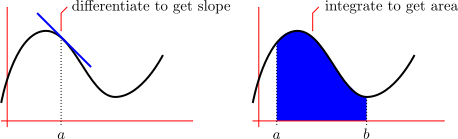
\includegraphics[height=4cm]{diff_int}
 \end{center}
\end{efig}
It is not immediately obvious that these two topics are related to each other.
However, as we shall see, they are indeed intimately linked.
\section{Definition of the Integral}\label{sec:intdef}

Arguably the easiest way to introduce integration is by considering the area between
the graph of a given function and the $x$-axis, between two specific vertical lines ---
such as is shown in the figure above. We'll follow this route by starting with
a motivating example.

%%%%%%%%%%%%%%%%%%%%%%%%%%%%%%%%%%%%%%%%%%%%%%%%%%%%%%%
\subsection{A Motivating Example}
%%%%%%%%%%%%%%%%%%%%%%%%%%%%%%%%%%%%%%%%%%%%%%%%%%%%%%%

Let us find the area under the curve $y=e^x$ (and above the $x$--axis)
for $0\le x\le 1$. That is, the area of
$\big\{\ (x,y)\ \big|\ 0\le y\le e^x$, $0\le x\le 1\ \big\}$.
\begin{efig}
 \begin{center}
  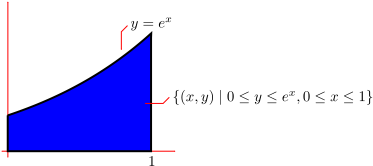
\includegraphics[height=4cm]{etox_area}
 \end{center}
\end{efig}
This area is equal to the
``definite integral''
\begin{align*}
  \text{Area} &= \int_0^1 e^x \dee{x}
\end{align*}
Do not worry about this notation or terminology just yet. We discuss
it at length below. In different applications this quantity will
have different interpretations --- not just area. For example, if $x$
is time and $e^x$ is your velocity at time $x$, then we'll see later
(in Example~\ref{eg:INTdistance}) that the specified area is the
net distance travelled between time $0$ and time $1$. After we finish
with the example, we'll mimic it to give a general definition of the
integral $\int_a^b f(x) \dee{x}$.

\begin{eg}\label{eg:INTexparea}
We wish to compute the area of $\big\{\ (x,y)\ \big|\ 0\le y\le e^x$, $0\le x\le
1\ \big\}$. We know, from our experience with $e^x$ in differential calculus,
that the curve $y=e^x$ is not easily written in terms of other simpler
functions, so it is very unlikely that we would be able to write the area as
a combination of simpler geometric objects such as triangles, rectangles or
circles.

So rather than trying to write down the area exactly, our strategy is to
approximate the area and then make our approximation more and more
precise\footnote{This should remind the reader of the approach taken to compute
the slope of a tangent line way way back at the start of differential
calculus.}. We choose\footnote{Approximating the area in this way leads to a
definition of integration that is called Riemann integration. This is the most
commonly used approach to integration. However we could also approximate the
area by using long thin horizontal strips. This leads to a definition of
integration that is called Lebesgue integration. We will not be covering
Lebesgue integration in these notes.} to approximate the area as a union of a
large number of tall thin (vertical) rectangles. As we take more and more
rectangles we get better and better approximations. Taking the limit as the
number of rectangles goes to infinity gives the exact area\footnote{If we want
to be more careful here, we should construct two approximations, one that is
always a little smaller than the desired area and one that is a little larger.
We can then take a limit using the Squeeze Theorem and arrive at the
exact area. More on this later.}.

As a warm up exercise, we'll now just use four rectangles. In Example
\ref{eg:INTexpareaB}, below, we'll consider an arbitrary number of rectangles
and then take the limit as the number of rectangles goes to infinity. So
\begin{itemize}
\item subdivide the interval $0\le x\le 1$ into $4$ equal subintervals
each of width $\nicefrac{1}{4}$, and
\item subdivide the area of interest into four corresponding
vertical strips, as in the figure below.
\end{itemize}
The area we want is exactly the sum of the areas of all four strips.
\begin{efig}
\begin{center}
   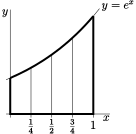
\includegraphics{earea1four}
\end{center}
\end{efig}
Each of these strips is almost, but not quite, a rectangle. While the bottom and
sides are fine (the sides are at right-angles to the base), the top of the strip
is not horizontal. This is where we must start to approximate. We can replace
each strip by a rectangle by just levelling off the top. But now we have to make
a choice --- at what height do we level off the top?

Consider, for example, the leftmost strip. On this strip, $x$ runs from $0$ to
$\nicefrac{1}{4}$. As $x$ runs from $0$ to $\nicefrac{1}{4}$, the height $y$
runs from $e^0$ to $e^{\nicefrac{1}{4}}$. It would be reasonable to choose the
height of the approximating rectangle to be somewhere between $e^0$ and
$e^{\nicefrac{1}{4}}$. Which
\vadjust{
\begin{efig}
\begin{center}
  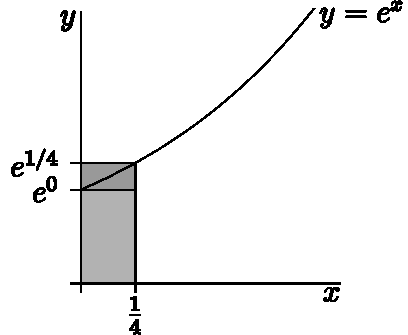
\includegraphics{earea3four}
\end{center}
\end{efig}
}
height should we choose? Well, actually it doesn't matter. When we eventually
take the limit of infinitely many approximating rectangles all of those
different choices give exactly the same final answer. We'll say more about this
later.

In this example we'll do two sample computations.
\begin{itemize}
\item For the first computation we approximate each slice by a rectangle
whose height is the height of the \emph{left} hand side of the slice.
\begin{itemize}
\item On the first slice, $x$ runs from $0$ to $\nicefrac{1}{4}$,
and the height $y$ runs from $e^0$, on the left hand side, to
$e^{\nicefrac{1}{4}}$, on the right hand side.

\item So we approximate the first slice by the rectangle of height
$e^0$ and width $\nicefrac{1}{4}$, and hence of area $\frac{1}{4}\,e^0
=\frac{1}{4}$.

\item On the second slice, $x$ runs from $\nicefrac{1}{4}$ to
$\nicefrac{1}{2}$, and the height $y$ runs from $e^{\nicefrac{1}{4}}$ and
$e^{\nicefrac{1}{2}}$.

\item So we approximate the second slice by the rectangle of height
$e^{\nicefrac{1}{4}}$ and width $\nicefrac{1}{4}$, and hence of area
$\frac{1}{4}\,e^{\nicefrac{1}{4}}$.

\item And so on.

\item All together, we approximate the area of interest by the sum
of the areas of the four approximating rectangles, which is
\begin{align*}
\big[1+ e^{\nicefrac{1}{4}} + e^{\nicefrac{1}{2}}
      +e^{\nicefrac{3}{4}}\big]\frac{1}{4}
=1.5124
\end{align*}

\item This particular approximation is called the ``left Riemann sum
approximation to $\int_0^1 e^x\dee{x}$ with $4$ subintervals''. We'll explain this
terminology later.

\item This particular approximation represents the shaded area
in the figure on the left below. Note that, because $e^x$ \emph{increases} as
$x$ increases, this approximation is definitely smaller than the true area.
\end{itemize}
\end{itemize}

\begin{efig}
\begin{center}
  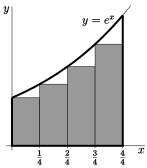
\includegraphics[width=0.45\textwidth]{earea4}\qquad
  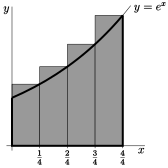
\includegraphics[width=0.45\textwidth]{earea4right}
\end{center}
\end{efig}

\begin{itemize}
\item For the second computation we approximate each slice by a rectangle
whose height is the height of the \emph{right} hand side of the slice.
\begin{itemize}
\item On the first slice, $x$ runs from $0$ to $\nicefrac{1}{4}$,
and the height $y$ runs from $e^0$, on the left hand side, to
$e^{\nicefrac{1}{4}}$, on the right hand side.

\item So we approximate the first slice by the rectangle of height
$e^{\nicefrac{1}{4}}$ and width $\nicefrac{1}{4}$, and hence of area
$\frac{1}{4}\,e^{\nicefrac{1}{4}}$.

\item On the second slice, $x$ runs from $\nicefrac{1}{4}$ to
$\nicefrac{1}{2}$, and the height $y$ runs from $e^{\nicefrac{1}{4}}$ and
$e^{\nicefrac{1}{2}}$.

\item So we approximate the second slice by the rectangle of height
$e^{\nicefrac{1}{2}}$ and width $\nicefrac{1}{4}$, and hence of area
$\frac{1}{4}\,e^{\nicefrac{1}{2}}$.

\item And so on.

\item All together, we approximate the area of interest by the sum
of the areas of the four approximating rectangles, which is
\begin{align*}
\big[e^{\nicefrac{1}{4}} + e^{\nicefrac{1}{2}}
      +e^{\nicefrac{3}{4}}+e^1\big]\frac{1}{4}
=1.9420
\end{align*}

\item This particular approximation is called the ``right Riemann sum
approximation to $\int_0^1 e^x\dee{x}$ with $4$ subintervals''.

\item This particular approximation represents the shaded area in the figure on
the right above. Note that, because $e^x$ \emph{increases} as $x$ increases,
this approximation is definitely larger than the true area.
\end{itemize}
\end{itemize}
\end{eg}

Now for the full computation that gives the exact area.
\begin{eg}\label{eg:INTexpareaB}
Recall that we wish to compute the area of $\big\{\ (x,y)\ \big|\ 0\le y\le
e^x$, $0\le x\le 1\ \big\}$ and that our strategy is to approximate this area by
the area of a union of a large number of very thin rectangles, and
then take the limit as the number of rectangles goes to infinity. In
Example~\ref{eg:INTexparea}, we used just four rectangles. Now we'll consider a
general number of rectangles, that we'll call $n$. Then we'll take the limit
$n\rightarrow\infty$. So
\begin{itemize}
\item pick a natural number $n$ and

\item subdivide the interval $0\le x\le 1$ into $n$ equal subintervals
each of width $\nicefrac{1}{n}$, and

\item subdivide the area of interest into corresponding thin strips, as in the
figure below.
\end{itemize}
The area we want is exactly the sum of the areas of all of the thin strips.
\begin{efig}
\begin{center}
   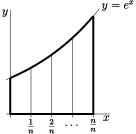
\includegraphics{earea1}
\end{center}
\end{efig}
Each of these strips is almost, but not quite, a rectangle. As in Example
\ref{eg:INTexparea}, the only problem is that the top is not horizontal. So we
approximate each strip by a rectangle, just by levelling off the top. Again, we
have to make a choice --- at what height do we level off the top?

Consider, for example, the leftmost strip. On this strip, $x$ runs from $0$ to
$\nicefrac{1}{n}$. As $x$ runs from $0$ to $\nicefrac{1}{n}$, the height $y$
runs from  $e^0$ to $e^{\nicefrac{1}{n}}$. It would be reasonable to choose the
height of the approximating rectangle to be somewhere between $e^0$ and
$e^{\nicefrac{1}{n}}$. Which height should we choose?

Well, as we said in Example \ref{eg:INTexparea}, it doesn't matter. We shall
shortly take the limit $n\rightarrow\infty$ and, in that limit, all of those
different choices give exactly the same final answer. We won't justify that
statement in this example, but there will be an (optional) section shortly that
provides the justification. For this example we just, arbitrarily, choose the
height of each rectangle to be the height of the graph $y=e^x$ at the smallest
value of $x$ in the corresponding strip\footnote{Notice that since $e^x$ is an
increasing function, this choice of heights means that each of our rectangles is
smaller than the strip it came from.}. The figure on the left below shows the
approximating rectangles when $n=4$ and the figure on the right shows the
approximating rectangles when $n=8$.
\begin{efig}
\begin{center}
  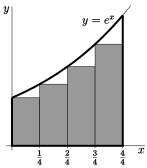
\includegraphics[width=0.45\textwidth]{earea4}\qquad
  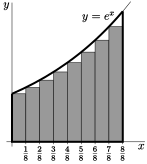
\includegraphics[width=0.45\textwidth]{earea5}
\end{center}
\end{efig}

Now we compute the approximating area when there are $n$ strips.
\begin{itemize}
\item We approximate the leftmost strip by a rectangle of height $e^0$. All of
the rectangles have width $\nicefrac{1}{n}$. So the leftmost rectangle has area
$\frac{1}{n}e^0$.

\item On strip number $2$, $x$ runs from $\frac{1}{n}$ to $\frac{2}{n}$. So the
smallest value of $x$ on strip number $2$ is $\frac{1}{n}$, and we approximate
strip number $2$ by a rectangle of height $e^{\nicefrac{1}{n}}$ and hence of
area $\frac{1}{n}e^{\nicefrac{1}{n}} $.

\item And so on.

\item On the last strip, $x$ runs from $\frac{n-1}{n}$ to $\frac{n}{n}=1$.
So the smallest value of $x$ on the last strip is $\frac{n-1}{n}$, and we
approximate the last strip by a rectangle of height $e^{\nicefrac{(n-1)}{n}}$
and hence of area $ \frac{1}{n}e^{\nicefrac{(n-1)}{n}} $.
\end{itemize}

The total area of all of the approximating rectangles is
\begin{align*}
\text{Total approximating area} &= \frac{1}{n}e^0
                                   + \frac{1}{n}e^{\nicefrac{1}{n}}
                                   + \frac{1}{n}e^{\nicefrac{2}{n}}
                                   + \frac{1}{n}e^{\nicefrac{3}{n}}
                                   + \cdots
                                   + \frac{1}{n}e^{\nicefrac{(n-1)}{n}} \\
&= \frac{1}{n}\Big( 1+ e^{\nicefrac{1}{n}}
+e^{\nicefrac{2}{n}}+e^{\nicefrac{3}{n}} +\cdots+
          e^{\nicefrac{(n-1)}{n}}\Big)
\end{align*}
Now the sum in the brackets might look a little intimidating because of all the
exponentials, but it actually has a pretty simple structure that can be easily
seen if we rename $e^{\nicefrac{1}{n}}=r$. Then
\begin{itemize}
\item the first term is 1 = $r^0$ and
\item the second term is $e^{\nicefrac{1}{n}}=r^1$ and
\item the third term is $e^{\nicefrac{2}{n}}=r^2$ and
\item the fourth term is $e^{\nicefrac{3}{n}}=r^3$ and
\item and so on and
\item the last term is $e^{\nicefrac{(n-1)}{n}}=r^{n-1}$.
\end{itemize}
So
\begin{align*}
\text{Total approximating area}
&= \frac{1}{n}\left( 1+ r +r^2 +\cdots+ r^{n-1}\right)
\end{align*}
The sum in brackets is known as a geometric sum and satisfies a nice simple
formula:
\begin{impeqn}[Geometric sum]\label{eq:INTgeomsum}
 \begin{align*}
1+ r +r^2 +\cdots+ r^{n-1} =\frac{r^n-1}{r-1} \qquad\text{provided $r\ne 1$}
\end{align*}
\end{impeqn}


\noindent The derivation of the above formula is not too difficult. So let's
derive it in a little aside.
\subsubsection*{Geometric Sum}
Denote the sum as
\begin{align*}
S &=
1 + r + r^2 + \cdots + r^{n-1}
\end{align*}
Notice that if we multiply the whole sum by $r$ we get back almost the same
thing:
\begin{align*}
rS&= r\left(1+ r +r^2 +\cdots+ r^{n-1}\right) \\
   &= r+ r^2+ r^3 +\cdots+ r^n
\end{align*}
This right hand side differs from the original sum $S$ only in that
\begin{itemize}
\item
the right hand side, which starts with ``$r+\,$'', is missing the ``$1+\,$'' 
that $S$ starts with, and
\item
the right hand side has an extra ``$+r^n\,$'' at the end that does
not appear in $S$.
\end{itemize}
That is
\begin{align*}
  rS & = S-1+r^n
\intertext{Moving this around a little gives}
  (r-1)S &= (r^n-1) \\
  S &= \frac{r^n-1}{r-1}
\end{align*}
as required. Notice that the last step in the manipulations only works providing $r \neq
1$ (otherwise we are dividing by zero).
\subsubsection*{Back to Approximating Areas}
Now we can go back to our area approximation armed with the above result about geometric
sums.
\begin{align*}\
\text{Total approximating area}
&= \frac{1}{n}\left( 1+ r +r^2 +\cdots+ r^{n-1}\right) \\
&= \frac{1}{n} \frac{r^n-1}{r-1} & \text{remember that $r=e^{1/n}$}\\
&= \frac{1}{n} \frac{e^{n/n} - 1}{e^{1/n}-1} \\
&= \frac{1}{n} \frac{e - 1}{e^{1/n}-1}
\end{align*}

To get the exact area\footnote{We haven't proved that this will give us the
exact area, but it should be clear that taking this limit will give us a lower
bound on the area. To complete things rigorously we also need an upper bound and
the squeeze theorem. We do this in the next optional subsection.} all we need to
do is make the approximation better and better by taking the limit $n\rightarrow
\infty$. The limit will look more familiar if we rename $\nicefrac{1}{n}$ to
$X$. As $n$ tends to infinity, $X$ tends to $0$, so
\begin{align*}
\text{Area}&=\lim_{n\rightarrow\infty} \frac{1}{n}\ \frac{e-1}{e^{1/n}-1} \\
&=(e-1)\lim_{n\rightarrow\infty} \frac{1/n}{e^{1/n}-1} \\
&=(e-1)\lim_{X\rightarrow 0} \frac{X}{e^X-1}
              &\text{(with $X=\nicefrac{1}{n}$)}
\end{align*}
Examining this limit we see that both numerator and denominator tend to zero as $X\to 0$,
and so we cannot evaluate this limit by computing the limits of the numerator and
denominator separately and then dividing the results. Despite this, the limit is not too
hard to evaluate; here we give two ways:
\begin{itemize}
 \item Perhaps the easiest way to compute the limit is by using
l'H\^opital's rule\footnote{If you do not recall L'H\^opital's rule and indeterminate
forms then we recommend you skim over your differential calculus notes on the topic.}.
Since both numerator and denominator go to zero, this is a $\nicefrac00$ indeterminate
form. Thus
\begin{align*}
\lim_{X\rightarrow 0} \frac{X}{e^X-1}
&=\lim_{X\rightarrow 0} \frac{\diff{}{X}X}{\diff{}{X}(e^X-1)}
=\lim_{X\rightarrow 0} \frac{1}{e^X}=1
\end{align*}
\item Another way\footnote{Say if you don't recall l'H\^opital's rule and have not had
time to revise it.} to evaluate the same limit is to observe that it can be massaged
into the form of the limit definition of the derivative. First notice that
\begin{align*}
\lim_{X\rightarrow 0} \frac{X}{e^X-1}
&= \left[\lim_{X\rightarrow 0} \frac{e^X-1}{X} \right]^{-1}
\end{align*}
provided this second limit exists and is nonzero. This second limit should look a little
familiar:
\begin{align*}
\lim_{X\rightarrow 0} \frac{e^X-1}{X}
&= \lim_{X\rightarrow 0} \frac{e^X-e^0}{X-0}
\end{align*}
which is just the definition of the derivative of $e^x$ at $x=0$. Hence we have
\begin{align*}
\lim_{X\rightarrow 0} \frac{X}{e^X-1}
&=\left[\lim_{X\rightarrow 0}\, \frac{e^X-e^0}{X-0} \right]^{-1} \\
&=\left[\diff{}{X}e^X\Big|_{X=0} \right]^{-1} \\
&=\left[e^X\big|_{X=0}\right]^{-1} \\
&=1
\end{align*}
\end{itemize}
So, after this short aside into limits, we may now conclude that
\begin{align*}
\text{Area}
&=(e-1)\lim_{X\rightarrow 0} \frac{X}{e^X-1} \\
&=e-1
\end{align*}
\addtocounter{theorem}{-1}%compensating for the impeqn env inside the example
\end{eg}
\addtocounter{theorem}{1}%compensating for the impeqn env inside the example


%%%%%%%%%%%%%%%%%%%%%%%%%%%%%%%%%%%%%%%%%%%%%%%%%%%%%%%
\subsection{Optional --- A More Rigorous Area Computation}
%%%%%%%%%%%%%%%%%%%%%%%%%%%%%%%%%%%%%%%%%%%%%%%%%%%%%%%
In Example~\ref{eg:INTexparea} above we considered the area of the region
$\big\{\ (x,y)\ \big|\ 0\le y\le e^x$, $0\le x\le 1\ \big\}$. We approximated that area
by
the area of a union of $n$ thin rectangles. We then claimed that upon taking
the number of rectangles to infinity, the approximation of the area became the
exact area. However we did not justify the claim. The purpose of this optional
section is to make that calculation rigorous.

The broad set-up is the same. We divide the region up into $n$ vertical strips,
each of width $\nicefrac1n$ and we then approximate those strips by rectangles.
However rather than an uncontrolled approximation, we construct two sets of
rectangles --- one set always smaller than the original area and one always
larger. This then gives us lower and upper bounds on the area of the region.
Finally we make use of the squeeze
theorem\footnote{
Recall that if we have 3 functions $f(x), g(x), h(x)$ that satisfy $f(x) \leq g(x) \leq
h(x)$ and we know that $\lim_{x \to a} f(x) = \lim_{x\to a} h(x) = L$ exists and is
finite, then the squeeze theorem tells us that $\lim_{x\to a} g(x) = L$.} to establish
the result.

\begin{itemize}
 \item To find our upper and lower bounds we make use of the fact that $e^x$ is an
increasing function. We know this because the derivative $\diff{}{x}e^x=e^x$  is always
positive. Consequently, the smallest and largest values of $e^x$ on the interval
$a\le x\le b$ are $e^a$ and $e^b$, respectively.

\item In particular, for $0\le x\le \nicefrac{1}{n}$,
$e^x$ takes values only between $e^0$ and $e^{\nicefrac{1}{n}}$.
As a result,  the first strip
\begin{align*}
\big\{\ (x,y)\ \big|\ 0\le x\le \nicefrac{1}{n},\ 0\le y\le e^x\ \big\}
\end{align*}
\begin{itemize}
\item contains the rectangle of $0\le x\le \nicefrac{1}{n}$, $0\le y\le e^0$
(the lighter rectangle in the figure on the left below) and
\item is contained in the rectangle $0\le x\le \nicefrac{1}{n}$, $0\le y\le
e^{\nicefrac{1}{n}}$
(the largest rectangle in the figure on the left below).
\end{itemize}
Hence
\begin{align*}
\frac{1}{n}e^{0}
\le {\rm Area}
  \big\{\ (x,y)\ \big|\ 0\le x\le \nicefrac{1}{n},\ 0\le y\le e^x\ \big\}
\le \frac{1}{n}e^{\nicefrac{1}{n}}
\end{align*}
\begin{efig}
\begin{center}
   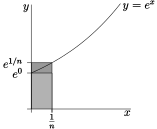
\includegraphics{earea3}\qquad 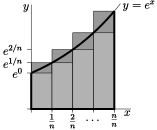
\includegraphics{earea6}
\end{center}
\end{efig}
\item Similarly, for the second, third, $\dots$, last strips,
as in the figure on the right above,
\begin{alignat*}{3}
\frac{1}{n}e^{\nicefrac{1}{n}}
&\le {\rm Area}\big\{\ (x,y)\ \big|\
             \nicefrac{1}{n}\le x\le \nicefrac{2}{n},\ 0\le y\le e^x\ \big\}
&\le \frac{1}{n}e^{\nicefrac{2}{n}}\\
%%
\frac{1}{n}e^{\nicefrac{2}{n}}
&\le {\rm Area}\big\{\ (x,y)\ \big|\
            \nicefrac{2}{n}\le x\le \nicefrac{3}{n},\ 0\le y\le e^x\ \big\}
&\le \frac{1}{n}e^{\nicefrac{3}{n}}\\
%%
\vdots\hskip0.5cm &\hskip3.5cm \vdots &\vdots\hskip0.7cm\\
%%
\frac{1}{n}e^{\nicefrac{(n-1)}{n}}
&\le {\rm Area}\big\{\ (x,y)\ \big|\
          \nicefrac{(n-1)}{n}\le x\le \nicefrac{n}{n},\ 0\le y\le e^x\ \big\}
&\ \le\frac{1}{n}e^{\nicefrac{n}{n}}
\end{alignat*}
\item
Adding these $n$ inequalities together gives
\begin{multline*}
\frac{1}{n}\left(1+e^{\nicefrac{1}{n}}+\cdots+e^{\nicefrac{(n-1)}{n}}\right)\\
\le {\rm Area}\big\{\ (x,y)\ \big|\ 0\le x\le 1,\ 0\le y\le e^x\ \big\}\\
\le \frac{1}{n}\left(e^{\nicefrac{1}{n}}+e^{\nicefrac{2}{n}}+\cdots+
         e^{\nicefrac{n}{n}}\right)
\end{multline*}
% \begin{align*}
% &\frac{1}{n}\left(1+e^{\nicefrac{1}{n}}+\cdots+e^{\nicefrac{(n-1)}{n}}\right)\\
% &\hskip1in\le {\rm Area}\big\{\ (x,y)\ \big|\ 0\le x\le 1,\ 0\le y\le e^x\ \big\}\\
% &\hskip2in\le \frac{1}{n}\left(e^{\nicefrac{1}{n}}+e^{\nicefrac{2}{n}}+\cdots+
%          e^{\nicefrac{n}{n}}\right)\\[0.05in]
% &\hskip2in= \frac{1}{n}e^{\nicefrac{1}{n}}\left(1+e^{\nicefrac{1}{n}}+\cdots
%                   +e^{\nicefrac{(n-1)}{n}}\right)
% \end{align*}

\item We can then recycle equation~\eqref{eq:INTgeomsum} with $r=e^{\nicefrac1n}$, so
that $r^n=\left(e^{\nicefrac{1}{n}}\right)^n=e$. Thus we have
\begin{align*}
\frac{1}{n}\frac{e-1}{e^{\nicefrac{1}{n}}-1}
\le {\rm Area}\big\{\ (x,y)\ \big|\ 0\le x\le 1,\ 0\le y\le e^x\ \big\}
\le \frac{1}{n}e^{\nicefrac{1}{n}}\frac{e-1}{e^{\nicefrac{1}{n}}-1}
\end{align*}
where we have used the fact that the upper bound is a simple multiple of the
lower bound:
\begin{align*}
\left(e^{\nicefrac{1}{n}}+e^{\nicefrac{2}{n}}+\cdots+
         e^{\nicefrac{n}{n}}\right)
&= e^{\nicefrac{1}{n}}\left(1+e^{\nicefrac{1}{n}}+\cdots
+e^{\nicefrac{(n-1)}{n}}\right).
\end{align*}

\item We now apply the squeeze theorem to the above inequalities. 
In particular, the limits of the lower and upper bounds are
$\lim_{n\rightarrow\infty}\frac{1}{n}\frac{e-1}{e^{\nicefrac{1}{n}}-1}$ and
$\lim_{n\rightarrow\infty}\frac{1}{n}e^{\nicefrac{1}{n}}\frac{e-1}{e^{\nicefrac{1}{n}}-1}$, respectively. As we did near the end of 
Example \ref{eg:INTexpareaB}, we make these limits look more familiar 
by renaming $\nicefrac{1}{n}$ to $X$. As $n$ tends to infinity, 
$X$ tends to $0$, so the limits of the lower and upper bounds are
\begin{align*}
\lim_{n\rightarrow\infty}\frac{1}{n}\frac{e-1}{e^{\nicefrac{1}{n}}-1}
&=(e-1)\lim_{X=\nicefrac{1}{n}\rightarrow 0}\frac{X}{e^X-1}
=e-1
\end{align*}
(by l'H\^opital's rule) and 
\begin{align*}
\lim_{n\rightarrow\infty}\frac{1}{n}e^{\nicefrac{1}{n}}\frac{e-1}{e^{\nicefrac{1}{n}}-1}
&=(e-1)\lim_{X=\nicefrac{1}{n}\rightarrow 0}\cdot \frac{Xe^X}{e^X-1}\\
&=(e-1)\lim_{X\to 0}e^X \cdot \lim_{X=\to 0}\frac{X}{e^X-1}\\
&=(e-1) \cdot 1 \cdot 1
\end{align*}
Thus, since the exact area is trapped between the lower and upper bounds, the squeeze
theorem then implies that
\begin{align*}
 \text{Exact area} &= e-1.
\end{align*}

\end{itemize}


%%%%%%%%%%%%%%%%%%%%%%%%%%%%%%%%%%%%%%%%%%%%%%%%%%%%%%%
\subsection{Summation Notation}\label{ssec sum notn}
%%%%%%%%%%%%%%%%%%%%%%%%%%%%%%%%%%%%%%%%%%%%%%%%%%%%%%%
As you can see from the above example (and the more careful rigorous computation), our
discussion of integration will involve a fair bit of work with sums of quantities. To
this end, we make a quick aside into summation notation. While one can work through the
material below without this notation, proper summation notation is well worth learning,
so we advise the reader to persevere.


Writing out the summands explicitly can become quite impractical --- for example, say we
need the sum of the first 11 squares:
\begin{align*}
  1 + 2^2 + 3^2 + 4^2+ 5^2 + 6^2 + 7^2 + 8^2 + 9^2 + 10^2 + 11^2
\end{align*}
This becomes tedious. Where the pattern is clear, we will often skip the middle few
terms and instead write
\begin{align*}
  1 + 2^2 + \cdots  + 11^2.
\end{align*}
A far more precise way to write this is using $\Sigma$ (capital-sigma) notation. For
example, we can write the above sum as
\begin{align*}
  \sum_{k=1}^{11} k^2
\end{align*}
This is read as
\begin{quote}
 The sum from $k$ equals 1 to 11 of $k^2$.
\end{quote}
More generally
\begin{notn}
Let $m\leq n$ be integers and let $f(x)$ be a function defined on the integers.
Then we write
\begin{align*}
  \sum_{k=m}^n f(k)
\end{align*}
to mean the sum of $f(k)$ for $k$ from $m$ to $n$:
\begin{align*}
  f(m) + f(m+1) + f(m+2) + \cdots + f(n-1) + f(n).
\end{align*}
Similarly we write
\begin{align*}
  \sum_{i=m}^n a_i
\end{align*}
to mean
\begin{align*}
  a_m+a_{m+1}+a_{m+2}+\cdots+a_{n-1}+a_n
\end{align*}
for some set of coefficients $\{ a_m, \ldots, a_n \}$.
\end{notn}

Consider the example
\begin{align*}
\sum_{k=3}^7 \frac{1}{k^2}=\frac{1}{3^2}+\frac{1}{4^2}+\frac{1}{5^2}+
\frac{1}{6^2}+\frac{1}{7^2}
\end{align*}
It is important to note that the right hand side of this expression evaluates to a
number\footnote{Some careful addition shows it is $\frac{46181}{176400}$.}; it does not
contain ``$k$''.  The summation index $k$  is just a ``dummy'' variable and
it does not have to be called $k$. For example
\begin{align*}
  \sum_{k=3}^7 \frac{1}{k^2}
  =\sum_{i=3}^7 \frac{1}{i^2}
  =\sum_{j=3}^7 \frac{1}{j^2}
  =\sum_{\ell=3}^7 \frac{1}{\ell^2}
\end{align*}
Also the summation index has no meaning outside the sum. For
example
\begin{align*}
k\sum_{k=3}^7 \frac{1}{k^2}
\end{align*}
has no mathematical meaning; it is gibberish.

A sum can be represented using summation notation in many different ways.
If you are unsure as to whether or not two summation notations
represent the same sum, just write out the first few terms and the last
couple of terms. For example,
\begin{align*}
\sum_{m=3}^{15} \frac{1}{m^2}
&=\overbrace{\frac{1}{3^2}}^{m=3}
  +\overbrace{\frac{1}{4^2}}^{m=4}
  +\overbrace{\frac{1}{5^2}}^{m=5}
  +\cdots
  +\overbrace{\frac{1}{14^2}}^{m=14}
  +\overbrace{\frac{1}{15^2}}^{m=15} \\
%\sum_{\ell=2}^{14} \frac{1}{(\ell+1)^2}
%&=\overbrace{\frac{1}{3^2}}^{\ell=2}
%  +\overbrace{\frac{1}{4^2}}^{\ell=3}
%  +\overbrace{\frac{1}{5^2}}^{\ell=4}
%  +\cdots
%  +\overbrace{\frac{1}{14^2}}^{\ell=13}
%  +\overbrace{\frac{1}{15^2}}^{\ell=14} \\
\sum_{m=4}^{16} \frac{1}{(m-1)^2}
&=\overbrace{\frac{1}{3^2}}^{m=4}
  +\overbrace{\frac{1}{4^2}}^{m=5}
  +\overbrace{\frac{1}{5^2}}^{m=6}
  +\cdots
  +\overbrace{\frac{1}{14^2}}^{m=15}
  +\overbrace{\frac{1}{15^2}}^{m=16}
\end{align*}
are equal.



Here is a theorem that gives a few rules for manipulating summation notation.
\begin{theorem}[Arithmetic of Summation Notation]\label{thm:INTsummationArith}
Let $n\ge m$ be integers. Then for all real numbers $c$ and $a_i,b_i$,
$m\le i\le n$.
\begin{enumerate}[(a)]
\item $\sum\limits_{i=m}^nca_i = c\bigg(\sum\limits_{i=m}^na_i\bigg)$
\item $\sum\limits_{i=m}^n(a_i+b_i) = \bigg(\sum\limits_{i=m}^na_i\bigg)
                                    + \bigg(\sum\limits_{i=m}^nb_i\bigg)$
\item $\sum\limits_{i=m}^n(a_i-b_i) = \bigg(\sum\limits_{i=m}^na_i\bigg)
                                    - \bigg(\sum\limits_{i=m}^nb_i\bigg)$
\end{enumerate}
\end{theorem}
\begin{proof}
We can prove this theorem by just writing out both sides of each equation,
and observing that they are equal, by the usual laws of arithmetic\footnote{Since all
the sums are finite, this isn't too hard. More care must be taken when the sums involve
an infinite number of terms. We will examine this in Chapter~\ref{chap seq ser}.}. For
example, for the first equation, the left and right hand sides are
\begin{align*}
\sum_{i=m}^nca_i = ca_m+ca_{m+1}+\cdots+ca_n
\quad\text{and}\quad
c\bigg(\sum\limits_{i=m}^na_i\bigg) = c(a_m+a_{m+1}+\cdots+a_n)
\end{align*}
They are equal by the usual distributive law. The ``distributive law''
is the fancy name for $c(a+b)=ca+cb$.
\end{proof}\goodbreak
Not many sums can be computed exactly\footnote{Of course, any finite sum can be computed
exactly --- just sum together the terms. What we mean by ``computed exactly'' in this
context, is that we can rewrite the sum as a simple, and easily
evaluated, formula involving the terminals of the sum. For example
\begin{align*}
  \sum_{k=m}^n r^k &= \frac{r^{n+1}-r^m}{r-1} &\text{provided $r\neq1$}
\end{align*}
No matter what finite integers we choose for $m$ and $n$, we can quickly compute the sum
in just a few arithmetic operations. On the other hand, the sums,
\begin{align*}
\sum_{k=m}^n \frac{1}{k} &&
\sum_{k=m}^n \frac{1}{k^2}
\end{align*}
cannot be expressed in such clean formulas (though you can rewrite them quite cleanly
using integrals). To explain more clearly we would need to go into a more detailed and
careful discussion that is beyond the scope of this course. }. Here are some that can.
The
first few are used a lot.
\begin{theorem}\label{thm:INTspecialSums}
\begin{enumerate}[(a)]
\item $\sum\limits_{i=0}^n ar^i = a\frac{1-r^{n+1}}{1-r}$, for all real numbers
$a$ and $r\ne 1$ and all integers $n\ge 0$.
\item $\sum\limits_{i=1}^n 1 = n$, for all integers $n\ge 1$.
\item $\sum\limits_{i=1}^n i = \frac{1}{2}n(n+1)$, for all integers $n\ge 1$.
\item $\sum\limits_{i=1}^n i^2 = \frac{1}{6}n(n+1)(2n+1)$, for all integers $n\ge 1$.
\item $\sum\limits_{i=1}^n i^3 = \Big[\frac{1}{2}n(n+1)\Big]^2$, for all integers $n\ge
1$.
\end{enumerate}
\end{theorem}
%%%%%%%%%%%%%%%%%%%%%%%%%%%%%%%%%%%%%%%%%%%%%%%%%%%%%%%
\subsubsection*{Proof of Theorem \ref{thm:INTspecialSums} (Optional)}
%%%%%%%%%%%%%%%%%%%%%%%%%%%%%%%%%%%%%%%%%%%%%%%%%%%%%%%
\begin{proof}
\begin{enumerate}[(a)]
\item The first sum is
\begin{align*}
\sum_{i=0}^n ar^i
=ar^0 + ar^1 + ar^2 + \cdots + ar^n
\end{align*}
which is just the left hand side of equation~\eqref{eq:INTgeomsum}, with $n$
replaced by $n+1$ and then multiplied by $a$.
\item The second sum is just $n$ copies of $1$ added together, so of course
the sum is $n$.
\item The third and fourth sums are discussed in the appendix of the CLP-1 text. In that discussion certain ``tricks'' are used to compute the
sums with only simple arithmetic. Those tricks do not easily generalise to the fifth sum.
\item[(c')] Instead of repeating that appendix, we'll derive the third sum
using a trick that
generalises to the fourth and fifth sums (and also to higher powers). The trick uses the
generating function\footnote{Generating functions are frequently used in mathematics to
analyse sequences and series, but are beyond the scope of the course. The interested
reader should take a look at ``Generatingfunctionology'' by Herb
Wilf. It is an excellent book and is also free to download.} $S(x)$:
\begin{impeqn}\label{eq:INTpowergenfnl}
\begin{align*}
S(x) = 1+x+x^2+\cdots+x^n &= \frac{x^{n+1}-1}{x-1}
\end{align*}
\end{impeqn}
Notice that this is just the geometric sum given by equation~\ref{eq:INTgeomsum} with $n$
replaced by $n+1$.

Now, consider the limit
\begin{align*}
\lim_{x\to 1} S(x) &= \lim_{x\to 1} \left(1+x+x^2+\cdots+x^n\right) = n+1 &\text{but
also}\\
&= \lim_{x\to 1} \frac{x^{n+1}-1}{x-1} &\text{now use l'H\^opital's rule}\\
&= \lim_{x\to 1} \frac{(n+1)x^n}{1} = n+1.
\end{align*}
This is not so hard (or useful). But now consider the derivative of $S(x)$:
\begin{align*}
S'(x) &= 1 +2x + 3x^2 + \cdots + n x^{n-1}\\
&= \diff{}{x} \left[\frac{x^{n+1}-1}{x-1}\right] & \text{use the quotient
rule}\\
&= \frac{(x-1)\cdot (n+1)x^n - (x^{n+1}-1)\cdot 1}{(x-1)^2} & \text{now clean
it up}\\
&= \frac{nx^{n+1}-(n+1)x^n+1}{(x-1)^2}.
\end{align*}
Hence if we take the limit of the above expression as $x\to 1$ we recover
\begin{align*}
\lim_{x\to 1} S'(x) &= 1 +2 +3+\cdots+n \\
&=\lim_{x\to 1} \frac{nx^{n+1}-(n+1)x^n+1}{(x-1)^2} & \text{now use l'H\^opital's rule}\\
&=\lim_{x\to 1} \frac{n(n+1)x^{n}-n(n+1)x^{n-1}}{2(x-1)}& \text{l'H\^opital's rule again}
\\
&=\lim_{x\to 1} \frac{n^2(n+1)x^{n-1}-n(n+1)(n-1)x^{n-2}}{2}\\
&= \frac{n^2(n+1) - n(n-1)(n+1)}{2} = \frac{n(n+1)}{2}
\end{align*}
as required. This computation can be done without l'H\^opital's rule, but the
manipulations required are a fair bit messier.

\intremark{%%%%%%%%%%%%%%%%%%%%%%%%%%%%

\noindent \emph{Alternate proof 1:}
By \eqref{eq:INTpowergenfnl},
\begin{align*}
1+2+3+\cdots+n&=\lim_{x\rightarrow 1}\diff{}{x}\Big[\frac{x^{n+1}-x}{x-1}\Big]\\
&=\lim_{x\rightarrow 1}\Big[\frac{((n+1)x^n-1)(x-1)-(x^{n+1}-x)1}{(x-1)^2}\Big]\\
&=\lim_{x\rightarrow 1}\Big[\frac{nx^{n+1}-(n+1)x^n+1}{(x-1)^2}\Big]\\
&=\lim_{x\rightarrow 1}\Big[\frac{n(n+1)x^n-n(n+1)x^{n-1}}{2(x-1)}\Big]\\
&=\lim_{x\rightarrow 1}\Big[\frac{n^2(n+1)x^{n-1}-n(n+1)(n-1)x^{n-2}}{2}\Big]\\
&=\frac{n^2(n+1)-n(n+1)(n-1)}{2}\\
&=\frac{(n+1)[n^2-n(n-1)]}{2}\\
&=\frac{n(n+1)}{2}
\end{align*}
as desired.



\noindent \emph{Alternate proof 2:}

We'll derive the third sum using a trick that generalises to the
fourth sum (and also to higher powers). The trick uses that
\begin{align*}
2\cdot a\cdot b=(a+b)^2-a^2-b^2
\end{align*}
Using this observation over and over,
\begin{align*}
2\cdot 1\cdot 1 &= (1+1)^2-1^2-1^2 \\
2\cdot 2\cdot 1 &= (2+1)^2-2^2-1^2 \\
2\cdot 3\cdot 1 &= (3+1)^2-3^2-1^2 \\
\vdots\hskip0.2in & \hskip0.5in\vdots \\
2\cdot (n-1)\cdot 1 &= (n-1+1)^2-(n-1)^2-1^2 \\
2\cdot n\cdot 1 &= (n+1)^2-n^2-1^2
\end{align*}
Now add all of these together. On the right hand sides, the $(1+1)^2$ of
the first row exactly cancels the $2^2$ of the second row, and the $(2+1)^2$
of the second row exactly cancels the $3^2$ of the third row, and so on.
So when we add all of the right hand sides together the only surviving
terms are the two $-1^2$'s of the first row, the $-1^2$ of rows two through
$n$ and the $(n+1)^2$ of row $n$. So
\begin{align*}
2(1+2+\cdots+n)=-1^2-n\cdot 1^2+(n+1)^2=n^2+n=n(n+1)
\end{align*}
Finally, just divide across by $2$.

\noindent \emph{Alternate proof 3:} uses the generating function
\begin{align}\label{eq:INTpowergenfnlexp}
e^{x}+e^{2x}+e^{3x}+\cdots+e^{nx}&=e^{x}\left(1+e^{x}+e^{2x}+e^{3x}+\cdots+e^{(n-1)x}
\right)
\notag\\
&=e^x\frac{e^{nx}-1}{e^x-1}\notag\\
&=\frac{e^{(n+1)x}-e^x}{e^x-1}
\end{align}
by \eqref{eq:INTgeomsum} with $r=e^x$. When we differentiate the
left hand side and then take the limit $x\rightarrow 0$ we get
\begin{align*}
\lim_{x\rightarrow 0}\diff{}{x}\big[e^{x}+e^{2x}+e^{3x}+\cdots+e^{nx}\big]
&=\lim_{x\rightarrow 0}\big[1e^{x}+2e^{2x}+3e^{3x}+\cdots+ne^{nx}\big] \\
&=1+2+3+\cdots+n
\end{align*}
which is exactly the sum that we are trying to evaluate. So, by \eqref{eq:INTpowergenfnl},
\begin{align*}
1+2+3+\cdots+n&=\lim_{x\rightarrow 0}\diff{}{x}\Big[\frac{e^{(n+1)x}-e^x}{e^x-1}\Big]\\
&=\lim_{x\rightarrow 0}
\Big[\frac{((n+1)e^{(n+1)x}-e^x)(e^x-1)-(e^{(n+1)x}-e^x)e^x}{(e^x-1)^2}\Big]\\
&=\lim_{x\rightarrow 0}
\Big[e^x\frac{ne^{(n+1)x}-(n+1)e^{nx}+1}{(e^x-1)^2}\Big]\\
&=\lim_{x\rightarrow 0}
\Big[\frac{ne^{(n+1)x}-(n+1)e^{nx}+1}{(e^x-1)^2}\Big]\\
&=\lim_{x\rightarrow 0}
\Big[\frac{n(n+1)e^{(n+1)x}-n(n+1)e^{nx}}{2(e^x-1)e^x}\Big]\\
&=\lim_{x\rightarrow 0}
\Big[\frac{n(n+1)e^{nx}-n(n+1)e^{(n-1)x}}{2(e^x-1)}\Big]\\
&=\lim_{x\rightarrow 0}
\Big[\frac{n^2(n+1)e^{nx}-n(n+1)(n-1)e^{(n-1)x}}{2 e^x}\Big]\\
&=\frac{n^2(n+1)-n(n+1)(n-1)}{2}\\
&=\frac{(n+1)[n^2-n(n-1)]}{2}\\
&=\frac{n(n+1)}{2}
\end{align*}


}%%%%%%%%%%%%%%%%%%%%%%%%%%%%%%%%%%%%%%%%%%%%%%%%%%%%%%%%%%%

\item The derivation of the fourth and fifth sums is similar to, but
even more tedious than, that of the third sum. One takes two or three
derivatives of the generating function.

\intremark{%%%%%%%%%%%%%%%%%%%%%%%%%%%%%%%%%%%%%%%%%%%%%%%
When we differentiate the
left hand side and then take the limit $x\rightarrow 1$ we get
\begin{align*}
&\lim_{x\rightarrow 1}\difftwo{}{x}\big[x+x^2+x^3+x^4+\cdots+x^n\big]\\
&\hskip1in
=\lim_{x\rightarrow 1}\big[2\cdot 1+3\cdot 2 x+4\cdot 3 x^2+\cdots+n(n-1)x^{n-2}\big] \\
&\hskip1in=2\cdot 1+3\cdot 2 +4\cdot 3 +\cdots+n(n-1) \\
&\hskip1in=\sum_{i=1}^n i(i-1)\\
&\hskip1in=\sum_{i=1}^n i^2 - \sum_{i=1}^n i\\
&\hskip1in=\sum_{i=1}^n i^2 - \frac{n(n+1)}{2}
\end{align*}
So the sum that we are trying to evaluate is $\frac{n(n+1)}{2}$ plus
\begin{align*}
\lim_{x\rightarrow 1}\difftwo{}{x}\Big[\frac{x^{n+1}-x}{x-1}\Big]
&=\lim_{x\rightarrow 1}\diff{}{x}\Big[\frac{nx^{n+1}-(n+1)x^n+1}{(x-1)^2}\Big] \\
&=\lim_{x\rightarrow 1}\Big[\frac{n(n+1)x^n-(n+1)nx^{n-1}}{(x-1)^2}
                           -2\frac{nx^{n+1}-(n+1)x^n+1}{(x-1)^3}\Big] \\
&=\lim_{x\rightarrow 1}\Big[\frac{(n+1)nx^{n-1}}{x-1}
                           -2\frac{nx^{n+1}-(n+1)x^n+1}{(x-1)^3}\Big] \\
&=\lim_{x\rightarrow 1}\Big[\frac{(n+1)nx^{n-1}(x-1)^2-2nx^{n+1}+2(n+1)x^n-2}
                                      {(x-1)^3}\Big] \\
&=\lim_{x\rightarrow 1}\Big[\frac{(n^2-n)x^{n+1}-2(n^2-1)x^n+(n+1)nx^{n-1}-2}
                                      {(x-1)^3}\Big] \\
&=\lim_{x\rightarrow 1}n(n^2-1)\Big[\frac{x^n-2x^{n-1}+x^{n-2}}
                                      {3(x-1)^2}\Big] \\
&=\lim_{x\rightarrow 1}n(n^2-1)\Big[\frac{x^{n-2}}{3}\Big] \\
&=\frac{n(n^2-1)}{3}
\end{align*}
So
\begin{align*}
\sum_{i=1}^n i^2 &= \frac{n(n^2-1)}{3} + \frac{n(n+1)}{2}
                 = \frac{n(n+1)[2(n-1)+3]}{6}
                 = \frac{n(n+1)(2n+1)}{6}
\end{align*}
as desired.
}%%%%%%%%%%%%%%%%%%%%%%%%%%%%%%%%%%%%%%%%%%%%%%%%%%%%%%%%%


\end{enumerate}

\end{proof}


%%%%%%%%%%%%%%%%%%%%%%%%%%%%%%%%%%%%%%%%%%%%%%%%%%%%%%%
\subsection{The Definition of the Definite Integral}\label{sec:defInt}
%%%%%%%%%%%%%%%%%%%%%%%%%%%%%%%%%%%%%%%%%%%%%%%%%%%%%%%

In this section we give a definition of the definite integral $\ds \int_a^b f(x)\dee{x}$
generalising the machinery we used in Example~\ref{eg:INTexparea}. But first some
terminology and a couple of remarks to better motivate the definition.
\begin{notn}
The symbol $\ds \int_a^b f(x)\dee{x}$ is read ``the definite integral of the function
$f(x)$ from $a$ to $b$''. The function $f(x)$ is called the integrand of $\int_a^b
f(x)\dee{x}$ and $a$ and $b$ are called\footnote{$a$ and $b$ are also called the bounds of integration.} the limits of integration. The interval $a\le x
\le b$ is called the interval of integration and is also called the domain of integration.
\end{notn}
Before we explain more precisely what the definite integral actually is, a few remarks
(actually --- a few interpretations) are in order.
\begin{itemize}
\item If $f(x)\ge 0$ and $a\le b$, one interpretation of the symbol
       $\ds \int_a^b f(x)\dee{x}$ is ``the area of the region $\big\{\ (x,y)\ \big|\
                                 a\le x\le b,\   0\le y\le f(x)\ \big\}$''.
      \begin{efig}
      \begin{center}
          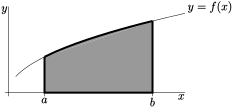
\includegraphics{areaSqrt}
      \end{center}
      \end{efig}
In this way we can rewrite the area in Example~\ref{eg:INTexparea} as the definite
integral $\int_0^1 e^x \dee{x}$.

\item This interpretation breaks down when either $a>b$ or $f(x)$ is not always positive,
but it can be repaired by considering ``signed areas''.

\item If $a\le b$, but $f(x)$ is not always positive, one interpretation of $\int_a^b
f(x)\dee{x}$ is ``the signed area between $y=f(x)$ and the $x$--axis for $a\le x\le b$''.
For ``signed area'' (which is also called the ``net area''), areas above the $x$--axis
count as positive while areas below the $x$--axis count as negative. In the example
below,
we have the graph of the function
      \begin{align*}
           f(x)=\begin{cases}
                   -1 & \text{if }1\le x\le 2 \\
                   2  & \text{if }2< x\le 4 \\
                   0 & \text{otherwise} \\
                \end{cases}
      \end{align*}
      The $2\times 2$ shaded square above the $x$--axis has signed area
      $+2\times 2=+4$. The $1\times 1$ shaded square below the $x$--axis has signed area
      $-1\times 1=-1$. So, for this $f(x)$,
      \begin{align*}
           \int_0^5 f(x)\dee{x} = +4-1=3
      \end{align*}
      \begin{efig}
      \begin{center}
          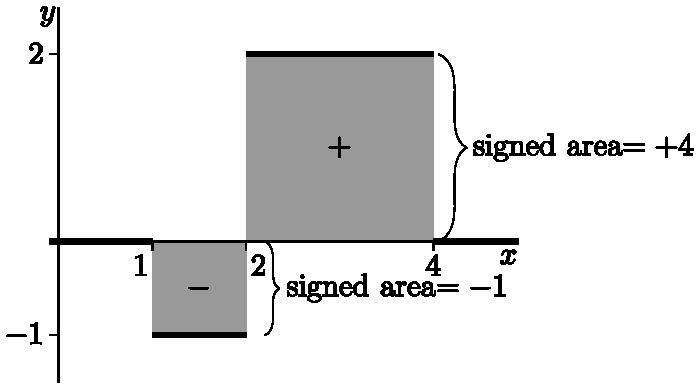
\includegraphics{signedArea}
      \end{center}
      \end{efig}
\item We'll come back to the case $b<a$ later.
\end{itemize}
We're now ready to define $\int_a^b f(x)\dee{x}$. The definition is a little involved,
but essentially mimics what we did in Example~\ref{eg:INTexparea} (which is why we did
the example before the definition). The main differences are that we replace the function
$e^x$ by a generic function $f(x)$ and we replace the interval from $0$ to $1$ by the
generic interval\footnote{We'll eventually allow $a$ and $b$ to be any two real numbers,
not even requiring $a<b$. But it is easier to start off assuming $a<b$, and that's what
we'll do.} from $a$ to $b$.
\begin{itemize}
\item We start by selecting any natural number $n$ and subdividing the interval from
$a$ to $b$ into $n$ equal subintervals. Each subinterval has width $\frac{b-a}{n}$.

\item Just as was the case in Example~\ref{eg:INTexparea} we will eventually take the
limit as $n\to\infty$, which squeezes the width of each subinterval down to zero.

\item For each integer $0\le i\le n$, define $x_i = a + i \cdot\frac{b-a}{n}$. Note that
this means that $x_0=a$ and $x_n = b$. It is worth keeping in mind that these numbers
$x_i$ do depend on $n$ even though our choice of notation hides this dependence.

\item Subinterval number $i$ is $x_{i-1} \leq x \leq
x_i$. In particular, on the first subinterval, $x$ runs from $x_0=a$
to $x_1=a+\frac{b-a}{n}$. On the second subinterval, $x$ runs from $x_1$ to
$x_2=a+2\frac{b-a}{n}$.
     \begin{efig}
     \begin{center}
         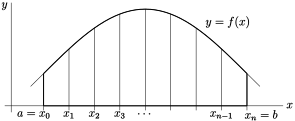
\includegraphics{intDecompE}
     \end{center}
     \end{efig}

\item On each subinterval we now pick $x_{i,n}^*$ between $x_{i-1}$ and $x_i$. We then
approximate $f(x)$ on the $i^\mathrm{th}$ subinterval by the constant function
$y=f(x_{i,n}^*)$. We include $n$ in the subscript to remind ourselves that these numbers
depend on $n$.

% We'll approximate $f$ on each subinterval by its value at some
% point of the subinterval. That is, for each $1\le i\le n$,
% we'll pick some $x_{i,n}^*$ between $x_{i-1}$ and $x_i$ and we'll approximate
% $f(x)$, for all $x$ between $x_{i-1}$ and $x_i$, by $f(x_{i,n}^*)$.
Geometrically, we're approximating the region
\begin{align*}
\big\{\ (x,y)\ \big|\
\text{$x$ is between $x_{i-1}$ and $x_i$, and $y$ is between $0$
 and $f(x)$} \ \big\}
\end{align*}
by the rectangle
\begin{align*}
\big\{\ (x,y)\ \big|\
\text{$x$ is between $x_{i-1}$ and $x_i$, and $y$ is between $0$
 and $f(x_{i,n}^*)$} \ \big\}
\end{align*}
     \begin{efig}
     \begin{center}
%          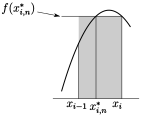
\includegraphics{rectApprox3}
         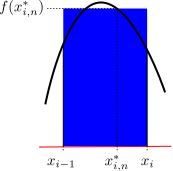
\includegraphics[height=45mm]{rect_approx_adr1}
     \end{center}
     \end{efig}
In Example~\ref{eg:INTexparea} we chose $x_{i,n}^* = x_{i-1}$ and so we
approximated the function $e^x$ on each subinterval by the value it took at the leftmost
point in that subinterval.

\item So, when there are $n$ subintervals our approximation to the signed
area between the curve $y=f(x)$ and the $x$--axis, with $x$ running from
$a$ to $b$, is
\begin{align*}
\sum_{i=1}^n f(x_{i,n}^*)\cdot \frac{b-a}{n}
\end{align*}
We interpret this as the signed area since the summands $f(x_{i,n}^*)\cdot\frac{b-a}{n}$
need not be positive.

\item Finally we define the definite integral by taking the limit of this sum as
$n\rightarrow\infty$.

\end{itemize}
Oof! This is quite an involved process, but we can now write down the definition we need.

\begin{defn}\label{def:INTintegral}
Let $a$ and $b$ be two real numbers and let $f(x)$ be a function that
is defined for all $x$ between $a$ and $b$. Then we define
\begin{align*}
\int_a^b f(x)\dee{x}
=\lim_{n\rightarrow\infty}\sum_{i=1}^n f(x_{i,n}^*)\cdot\frac{b-a}{n}
\end{align*}
when the limit exists and takes the same value for all choices of
the $x_{i,n}^*$'s. In this case, we say that $f$ is integrable on the
interval from $a$ to $b$.
\end{defn}
Of course, it is not immediately obvious when this limit should exist. Thankfully it is
easier for a function to be ``integrable'' than it is for it to be ``differentiable''.
\begin{theorem}\label{thm:integrable}
 Let $f(x)$ be a function on the interval $[a,b]$. If
\begin{itemize}
 \item $f(x)$ is continuous on $[a,b]$, or
 \item $f(x)$ has a finite number of jump discontinuities on $[a,b]$ (and is otherwise
continuous)
\end{itemize}
then $f(x)$ is integrable on $[a,b]$.
\end{theorem}
We will not justify this theorem. But a slightly weaker statement is proved
in (the optional) Section~\ref{ssec careful defn}. Of course this does not tell us how to
actually evaluate any definite integrals --- but we will get to that in time.

Some comments:
\begin{itemize}
 \item Note that, in Definition \ref{def:INTintegral}, we allow $a$ and $b$ to
be any two real numbers. We do not require that $a<b$. That is, even when
$a>b$, the symbol $\int_a^b f(x)\dee{x}$ is still defined by the formula
of Definition \ref{def:INTintegral}. We'll get an interpretation for
$\int_a^b f(x)\dee{x}$, when $a>b$, later.

\item It is important to note that the definite integral $\int_a^b f(x)\dee{x}$
represents a number, not a function of $x$. The integration variable $x$
is another ``dummy'' variable, just like the summation index $i$ in
$\sum_{i=m}^n a_i$ (see Section~\ref{ssec sum notn}). The integration variable does not
have to be called $x$.
For example
\begin{align*}
\int_a^b f(x)\dee{x} = \int_a^b f(t)\dee{t} = \int_a^b f(u)\dee{u}
\end{align*}
Just as with summation variables, the integration variable $x$
has no meaning outside of $f(x)\dee{x}$. For example
\begin{align*}
x\int_0^1 e^x\dee{x}\qquad\text{and}\qquad  \int_0^x e^x\dee{x}
\end{align*}
are both gibberish.
\end{itemize}

The sum inside definition~\ref{def:INTintegral} is named after Bernhard
Riemann\footnote{Bernhard Riemann was a 19th century German mathematician who
made
extremely important contributions to many different areas of mathematics --- far
too
many to list here. Arguably two of the most important (after Riemann sums) are
now
called Riemann surfaces and the Riemann hypothesis (he didn't name them after
himself).}
who made the first rigorous definition of the definite integral and so placed
integral
calculus on rigorous footings.
\begin{defn}\label{def:INTthreeRiemannSums}
The sum $\ds $ inside definition~\ref{def:INTintegral}
\begin{align*}
\sum_{i=1}^n f(x_{i,n}^*)\,\frac{b-a}{n}
\end{align*}
is called a Riemann sum. It is also often written as
\begin{align*}
\sum_{i=1}^n f(x_i^*)\,\De x
\end{align*}
where $\De x = \frac{b-a}{n}$.
\begin{itemize}


\item If we choose each $x_{i,n}^* = x_{i-1}=a+(i-1)\frac{b-a}{n}$ to be the
left hand end point of the $i^{\rm th}$ interval, $[x_{i-1},x_i]$,
we get the approximation
\begin{align*}
\sum_{i=1}^n f\left(a+(i-1)\frac{b-a}{n}\right)\,\frac{b-a}{n}
\end{align*}
which is called the ``left Riemann sum approximation to
$\int_a^b f(x)\dee{x}$ with $n$ subintervals''. This is the approximation used
in
Example~\ref{eg:INTexparea}.

\item In the same way, if we choose $x_{i,n}^* = x_{i}=a+i\frac{b-a}{n}$ we
obtain
the approximation
\begin{align*}
\sum_{i=1}^n f\left(a+i\frac{b-a}{n}\right)\,\frac{b-a}{n}
\end{align*}
which is called the ``right Riemann sum approximation to
$\int_a^b f(x)\dee{x}$ with $n$ subintervals''. The word ``right'' signifies
that, on each
subinterval $[x_{i-1},x_i]$ we approximate $f$ by its value at the right--hand
end--point,
$x_i=a+i\frac{b-a}{n}$, of the subinterval.


\item A third commonly used approximation is
\begin{align*}
\sum_{i=1}^n f\left(a+(i-\nicefrac12)\frac{b-a}{n}\right)\,\frac{b-a}{n}
\end{align*}
which is called the ``midpoint Riemann sum approximation to
$\int_a^b f(x)\dee{x}$ with $n$ subintervals''. The word ``midpoint''
signifies that, on each subinterval $[x_{i-1},x_i]$ we approximate $f$
by its value at the midpoint, $\frac{x_{i-1}+x_i}{2}
=a+(i-\nicefrac{1}{2})\frac{b-a}{n}$, of the subinterval.

\end{itemize}
\end{defn}


In order to compute a definite integral using Riemann sums we need to be able to
compute
the limit of the sum as the number of summands goes to infinity. This approach
is not
always feasible and we will soon arrive at other means of computing definite
integrals
based on antiderivatives. However, Riemann sums also provide us with a good
means of
approximating definite integrals --- if we take $n$ to be a large, but finite,
integer,
then the corresponding Riemann sum can be a good approximation of the definite
integral.
Under certain circumstances this can be strengthened to give rigorous bounds on
the
integral. Let us revisit Example~\ref{eg:INTexparea}.
\begin{eg}
Let's say we are again interested in the integral $\int_0^1 e^x\dee{x}$. We can
follow
the same procedure as we used previously to construct Riemann sum
approximations. However
since the integrand $f(x)=e^x$ is an increasing function, we can make our
approximations
into upper and lower bounds without much extra work.

More precisely, we approximate $f(x)$ on each subinterval $x_{i-1}\le x\le x_i$
\begin{itemize}
\item by its smallest value on the subinterval, namely $f(x_{i-1})$, when
we compute the left Riemann sum approximation and

\item by its largest value on the subinterval, namely $f(x_i)$, when we
compute the right Riemann sum approximation.
\end{itemize}
This is illustrated in the two figures below. The shaded region in the
left hand figure is the left Riemann sum approximation and the
shaded region in the right hand figure is the right Riemann sum approximation.
\begin{efig}
\begin{center}
   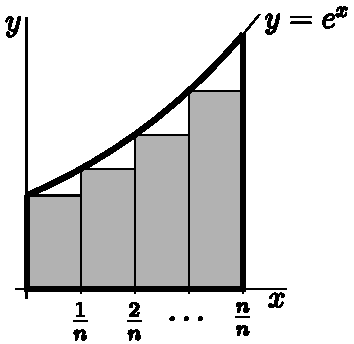
\includegraphics{earea7}\qquad
   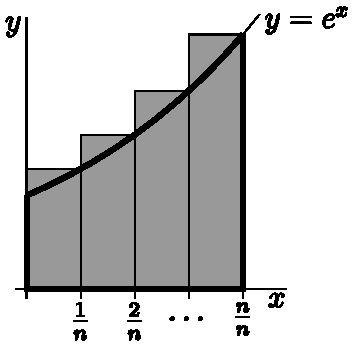
\includegraphics{earea8}
\end{center}
\end{efig}
We can see that exactly because $f(x)$ is increasing, the left Riemann sum
describes an area smaller than the definite integral while the right Riemann sum
gives an
area larger\footnote{When a function is decreasing the situation is reversed ---
the
left Riemann sum is always larger than the integral while the right Riemann sum
is
smaller than the integral. For more general functions that both increase and
decrease it
is perhaps easiest to study each increasing (or decreasing) interval
separately.} than
the integral.



When we approximate the integral $\int_0^1 e^x\dee{x}$ using $n$ subintervals,
then, on interval number~$i$,
\begin{itemize}\itemsep1pt \parskip0pt \parsep0pt %\itemindent-15pt
\item $x$ runs from $\frac{i-1}{n}$ to $\frac{i}{n}$ and
\item $y=e^x$ runs from $e^{\nicefrac{(i-1)}{n}}$, when $x$ is
at the left hand end point of the interval, to $e^{\nicefrac{i}{n}}$,
when $x$ is at the right hand end point of the interval.
\end{itemize}
Consequently, the left Riemann sum approximation to $\int_0^1 e^x\dee{x}$
is $\sum_{i=1}^n e^{\nicefrac{(i-1)}{n}}\,\frac{1}{n}$ and the
right Riemann sum approximation is
$\sum_{i=1}^n e^{\nicefrac{i}{n}}\cdot\frac{1}{n}$. So
\begin{align*}
\sum_{i=1}^n e^{\nicefrac{(i-1)}{n}}\,\frac{1}{n}
\ \le\ \int_0^1 e^x\dee{x}\ \le\
\sum_{i=1}^n e^{\nicefrac{i}{n}}\cdot\frac{1}{n}
\end{align*}
Thus
$L_n=\sum_{i=1}^n e^{\nicefrac{(i-1)}{n}}\,\frac{1}{n}$, which for any $n$
can be evaluated by computer, is a lower bound on the exact value of
$\int_0^1 e^x\dee{x}$ and
$R_n=\sum_{i=1}^n e^{\nicefrac{i}{n}}\,\frac{1}{n}$, which for any $n$
can also be evaluated by computer, is an upper bound on the exact value
of  $\int_0^1 e^x\dee{x}$. For example, when $n=1000$, $L_n= 1.7174$ and
$R_n=1.7191$ (both to four decimal places) so that, again to four
decimal places,
\begin{align*}
1.7174 \le \int_0^1 e^x\dee{x} \le 1.7191
\end{align*}
Recall that the exact value is $e-1 = 1.718281828\dots$.
\end{eg}

%%%%%%%%%%%%%%%%%%%%%%%%%%%%%%%%%%%%%%%%%%%%%%%%%%%%%%%
\subsection{Using Known Areas to Evaluate Integrals}\label{ssec knownareas}
%%%%%%%%%%%%%%%%%%%%%%%%%%%%%%%%%%%%%%%%%%%%%%%%%%%%%%%
One of the main aims of this course is to build up general machinery for
computing
definite integrals (as well as interpreting and applying them). We shall start
on this
soon, but not quite yet. We have already seen one concrete, if laborious, method
for
computing definite integrals --- taking limits of Riemann sums as we did in
Example~\ref{eg:INTexparea}. A second method, which will work for some special
integrands, works by interpreting the definite integral as ``signed area''.
This
approach will work nicely when the area under the curve decomposes into simple
geometric
shapes like triangles, rectangles and circles. Here are some examples of this
second method.

\begin{eg}
The integral $\int_a^b 1\dee{x}$ (which is also written as just $\int_a^b\dee{x}$) is
the
area of
the shaded rectangle (of width $b-a$ and height $1$) in the figure on
the right below. So
\begin{align*}
\int_a^b\dee{x} = (b-a)\times (1)=b-a\qquad\qquad
\raisebox{-0.5\height}{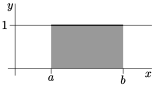
\includegraphics{areaRect}}
\end{align*}
\end{eg}


\begin{eg}\label{eg:INTtriangle}
Let $b>0$.
The integral $\int_0^b x\dee{x}$  is the area of
the shaded triangle (of base $b$ and of height $b$) in the figure on
the right below. So
\begin{align*}
\int_0^b x\dee{x} = \frac{1}{2}b\times b=\frac{b^2}{2}\qquad\qquad
\raisebox{-0.5\height}{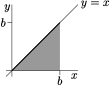
\includegraphics{areaX}}
\end{align*}
The integral $\int_{-b}^0 x\dee{x}$  is the signed area of
the shaded triangle (again of base $b$ and of height $b$) in the figure on
the right below. So
\begin{align*}
\int_{-b}^0 x\dee{x} = -\frac{b^2}{2}\qquad\qquad
\raisebox{-0.5\height}{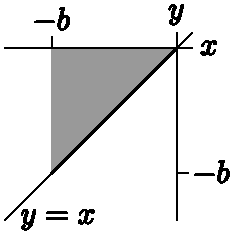
\includegraphics{areaMX}}
\end{align*}
\end{eg}
Notice that it is very easy to extend this example to the integral $\int_0^b
c x\dee{x}$ for any real numbers $b,c>0$ and find
\begin{align*}
\int_0^b c x\dee{x} &= \frac{c}{2} b^2.
\end{align*}

\begin{eg}\label{eg:INTtriangleB}
In this example, we shall evaluate $\int_{-1}^1 \left(1-|x|\right)\dee{x}$.
Recall that
\begin{align*}
|x|=\begin{cases} -x &\text{if $x\le 0$}\\
                   x &\text{if $x\ge 0$}
    \end{cases}
\end{align*}
so that
\begin{align*}
1-|x|=\begin{cases} 1+x &\text{if $x\le 0$}\\
                    1-x &\text{if $x\ge 0$}
    \end{cases}
\end{align*}
To picture the geometric figure whose area the integral represents
observe that
\begin{itemize}\itemsep1pt \parskip0pt \parsep0pt %\itemindent-15pt
\item
at the left hand end of the domain of integration $x=-1$ and
the integrand $1-|x|=1-|-1|=1-1=0$ and
\item
as $x$ increases from $-1$ towards $0$, the integrand $1-|x|=1+x$ increases
linearly, until
\item
when $x$ hits $0$ the integrand hits  $1-|x|=1-|0|=1$ and then
\item
as $x$ increases from $0$, the integrand $1-|x|=1-x$ decreases
linearly, until
\item
when $x$ hits $+1$, the right hand end of the domain of integration, the
integrand hits
$1-|x|=1-|1|=0$.
\end{itemize}
So the integral $\int_{-1}^1 \left(1-|x|\right)\dee{x}$  is the area of
the shaded triangle (of base $2$ and of height $1$) in the figure on
the right below and
\begin{align*}
\int_{-1}^1 \left(1-|x|\right)\dee{x} = \frac{1}{2}\times 2\times 1 =
1\qquad\qquad
\raisebox{-0.5\height}{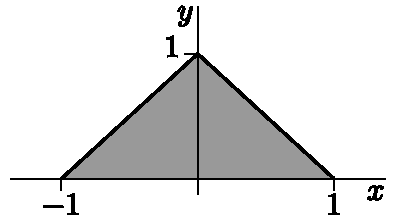
\includegraphics{areaAbs}}
\end{align*}
\end{eg}

\vskip0.15in
\begin{eg}\label{eg quarter circle}
The integral $\int_0^1 \sqrt{1-x^2}\dee{x}$  has integrand $f(x)=\sqrt{1-x^2}$.
So it represents the area under $y=\sqrt{1-x^2}$ with $x$ running from
$0$ to $1$. But we may rewrite
\begin{align*}
  y&=\sqrt{1-x^2} &\text{as}&& x^2+y^2&= 1, y\geq 0
\end{align*}
But this is the (implicit) equation for a circle --- the extra condition that
$y\geq0$
makes it the equation for the semi-circle centred at the origin with radius 1
lying on
and above the $x$-axis. Thus the integral represents the area of the quarter
circle of
radius $1$, as shown in the figure on the right below. So
\begin{align*}
\int_0^1 \sqrt{1-x^2}\dee{x} = \frac{1}{4}\pi(1)^2 = \frac{\pi}{4}\qquad\qquad
\raisebox{-0.5\height}{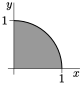
\includegraphics{areaCirc}}
\end{align*}
\end{eg}

This next one is a little trickier and relies on us knowing the symmetries of the
sine
function.
\begin{eg}
The integral $\int_{-\pi}^\pi \sin x\dee{x}$  is the signed area of
the shaded region in the figure on the right below. It naturally splits into
two
regions, one on either side of the $y$-axis. We don't know the formula for the
area of
either of these regions (yet), however the two regions are very nearly the same.
In
fact, the part of the
shaded region below the $x$--axis is exactly the reflection, in the $x$--axis,
of the part of the shaded region above the $x$--axis. So the signed area
of part of the shaded region below the $x$--axis is the negative of the
signed area of part of the shaded region above the $x$--axis and
\begin{align*}
\int_{-\pi}^\pi \sin x\dee{x} = 0\qquad\qquad
\raisebox{-0.4\height}{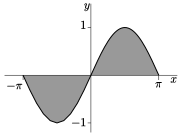
\includegraphics{areaSin}}
\end{align*}
\end{eg}

%%%%%%%%%%%%%%%%%%%%%%%%%%%%%%%%%%%%%%%%%%%%%%%%%%%%%%%
\subsection{Another Interpretation for Definite Integrals}\label{ssec velocity}
%%%%%%%%%%%%%%%%%%%%%%%%%%%%%%%%%%%%%%%%%%%%%%%%%%%%%%%

So far, we have only a single interpretation\footnote{If this were the only
interpretation
then integrals would be a nice mathematical curiosity and unlikely to be the
core
topic of a large first year mathematics course.} for definite integrals ---
namely areas
under graphs. In the following example, we develop a second interpretation.
\begin{eg}\label{eg:INTdistance}
Suppose that a particle is moving along the $x$--axis
and suppose that at time $t$ its velocity is $v(t)$ (with $v(t)>0$
indicating rightward motion and $v(t)<0$ indicating leftward motion).
What is the change in its $x$--coordinate between time $a$ and time $b>a$?

We'll work this out using a procedure similar to our definition of the
integral. First pick a natural number $n$ and divide the time interval from $a$
to $b$ into $n$ equal subintervals, each of width $\frac{b-a}{n}$. We are
working our way
towards a Riemann sum (as we have done several times above) and so we will
eventually
take the limit $n\rightarrow\infty$.
\begin{itemize}
\item The first time interval runs from $a$ to $a+\frac{b-a}{n}$. If we think of
$n$ as
some large number, the width of this interval, $\frac{b-a}{n}$ is very small and
over
this time interval, the velocity does not change very much. Hence we can
approximate the
velocity over the first subinterval as being essentially constant at its value
at the
start of the time interval --- $v(a)$. Over the subinterval the $x$-coordinate
changes by
velocity times time, namely $v(a) \cdot \frac{b-a}{n}$.

\item Similarly, the second  interval runs from time $a+\frac{b-a}{n}$
to time $a+2\frac{b-a}{n}$. Again, we can assume that the velocity does not
change
very much and so we can approximate the velocity as being essentially constant
at its
value at the start of the subinterval --- namely
$v\left(a+\frac{b-a}{n}\right)$. So
during the second subinterval the particle's
$x$--coordinate changes by approximately $v\left(a+\frac{b-a}{n}\right)
\frac{b-a}{n}$.
\item In general, time subinterval number $i$ runs from $a+(i-1)\frac{b-a}{n}$
to $a+i\frac{b-a}{n}$ and during this subinterval the particle's $x$--coordinate
changes, essentially, by
\begin{align*}
v\left(a+(i-1)\frac{b-a}{n}\right)  \frac{b-a}{n}.
\end{align*}

\end{itemize}
So the net change in $x$--coordinate from time $a$ to time $b$ is approximately
\begin{align*}
&v(a)\,\frac{b-a}{n} + v\Big(a+\frac{b-a}{n}\Big)\,\frac{b-a}{n} +\cdots
+v\Big(a+(i-1)\frac{b-a}{n}\Big)\,\frac{b-a}{n} + \cdots \\
&\hskip3.5in
+v\Big(a+(n-1)\frac{b-a}{n}\Big)\,\frac{b-a}{n} \\
&= \sum_{i=1}^n v\Big(a+(i-1)\frac{b-a}{n}\Big)\,\frac{b-a}{n}
\end{align*}
This is exactly the left Riemann sum approximation to the integral of $v$
from $a$ to $b$ with $n$ subintervals. The limit as $n\rightarrow\infty$
is exactly the definite integral $\int_a^b v(t)\dee{t}$. Following tradition,
we have called the (dummy) integration variable $t$ rather than $x$ to
remind us that it is time that is running from $a$ to $b$.

The conclusion of the above discussion is that if a particle is moving
along the $x$--axis and its $x$--coordinate and velocity at time $t$ are
$x(t)$ and $v(t)$, respectively, then, for all $b>a$,
\begin{align*}
x(b)  - x(a) = \int_a^b v(t)\dee{t}.
\end{align*}

\end{eg}

%It is generally tiresome in the extreme to actually evaluate an integral
%directly using the definition. Fortunately, in practice, one virtually
%never has to do so.


%%%%%%%%%%%%%%%%%%%%%%%%%%%%%%%%%%%%%%%%%%%%%%%%%%%%%%%%%
\subsection{Optional --- Careful Definition of the Integral}\label{ssec
careful defn}
%%%%%%%%%%%%%%%%%%%%%%%%%%%%%%%%%%%%%%%%%%%%%%%%%%%%%%%%%
In this optional section we give a more mathematically rigorous definition of
the definite
integral $\ds \int_a^b f(x)\dee{x}$. Some textbooks use a sneakier, but
equivalent,
definition. The integral will be defined as the limit of a family of
approximations to the
area between the graph of $y=f(x)$ and the $x$--axis, with $x$ running from $a$
to $b$.
We will then show conditions under which this limit is guaranteed to exist. We
should
state up front that these conditions are more restrictive than is strictly
necessary ---
this is done so as to keep the proof accessible.

The family of approximations needed is slightly more general than that used to
define
Riemann sums in the previous sections, though it is quite similar. The main
difference is
that we do not require that all the subintervals have the same size.
\begin{itemize}
\item We start by selecting a positive integer $n$. As was the case previously,
this will
be the number of subintervals used in the approximation and eventually we will
take the
limit as $n \to \infty$.

\item Now subdivide the interval from $a$ to $b$ into $n$ subintervals by
selecting $n+1$
values of $x$ that obey
\begin{align*}
a=x_0<x_1<x_2<\cdots<x_{n-1}<x_n=b.
\end{align*}
The subinterval number $i$ runs from $x_{i-1}$ to $x_i$. This formulation does
not require the subintervals to have the same size. However we will eventually
require
that the widths of the subintervals shrink towards zero as $n\to\infty$.

\item Then for each subinterval we select a value of $x$ in that interval. That
is, for
$i=1,2,\dots,n$, choose $x_i^*$ satisfying $x_{i-1} \leq x_i^* \leq x_i$. We
will use
these values of $x$ to help approximate $f(x)$ on each subinterval.

\item The area between the graph of $y=f(x)$ and the $x$--axis, with $x$ running
\vadjust{
     \begin{efig}
     \begin{center}
         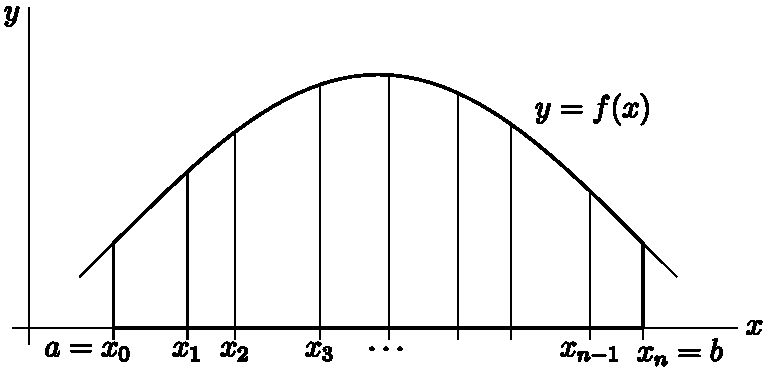
\includegraphics{intDecompU}
     \end{center}
     \end{efig}
}
from $x_{i-1}$ to $x_i$, i.e. the contribution,
$\int_{x_{i-1}}^{x_i} f(x)\dee{x}$, from interval number $i$ to the integral,
is approximated by the area of a rectangle. The rectangle has width
$x_i-x_{i-1}$ and height $f(x_i^*)$.
\begin{efig}
\begin{center}
%     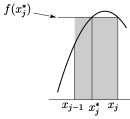
\includegraphics{rectApprox}
      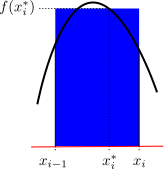
\includegraphics{rect_approx_adr2}
\end{center}
\end{efig}
\item Thus the approximation to the integral, using all $n$ subintervals, is
\begin{align*}
\int_a^b f(x)\dee{x}
\approx f(x_1^*)[x_1-x_0]+f(x_2^*)[x_2-x_1]+\cdots+ f(x_n^*)[x_n-x_{n-1}]
\end{align*}
\item Of course every different choice of $n$ and $x_1,x_2,\dots,x_{n-1}$
and $x_1^*, x_2^*,\dots,x_n^*$ gives a different approximation. So to
simplify the
discussion that follows, let us denote a particular choice of all these numbers
by $\bbbp$:
\begin{align*}
\bbbp=\left(n,x_1,x_2,\cdots,x_{n-1},x_1^*, x_2^*, \cdots, x_n^*\right).
\end{align*}
Similarly let us denote the resulting approximation by $\cI(\bbbp)$:
\begin{align*}
\cI(\bbbp)=f(x_1^*)[x_1-x_0]+f(x_2^*)[x_2-x_1]+\cdots+ f(x_n^*)[x_n-x_{n-1}]
\end{align*}

\item We claim that, for any reasonable\footnote{We'll be more precise about
what ``reasonable'' means shortly.} function $f(x)$, if you take any
reasonable\footnote{Again, we'll explain this ``reasonable'' shortly} sequence
of
these
approximations you always get the exactly the same limiting value. We define
$\int_a^b f(x) \dee{x}$ to be this limiting value.

\item Let's be more precise. We can take the limit of these approximations in
two equivalent ways. Above we did this by taking the number of subintervals $n$
to infinity. When we did this, the width of all the subintervals went to zero.
With the formulation we are now using, simply taking the number of subintervals
to be very large does not imply that they will all shrink in size. We could
have
one very large subinterval and a large number of tiny ones. Thus we take the
limit we need by taking the width of the subintervals to zero. So for any
choice
$\bbbp$, we define
\begin{align*}
M(\bbbp)=\max\big\{ x_1-x_0\ ,\  x_2-x_1\ ,\  \cdots\ ,\  x_n-x_{n-1}\big\}
\end{align*}
that is the maximum width of the subintervals used in the approximation
determined by
$\bbbp$. By forcing the maximum width to go to zero, the widths of all the
subintervals
go to zero.
\item We then define the definite integral as the limit
\begin{align*}
\int_a^b f(x)\dee{x}=\lim_{M(\bbbp)\rightarrow 0}\cI(\bbbp).
\end{align*}
\end{itemize}
Of course, one is now left with the question of determining when the above
limit
exists.
A proof of the very general conditions which guarantee existence of this limit
is beyond
the scope of this course, so we instead give a weaker result (with stronger
conditions)
which is far easier to prove.


For the rest of this section, assume
\begin{itemize}
 \item that $f(x)$ is continuous for $a\le x\le b$,
 \item that $f(x)$ is differentiable for $a<x<b$, and
 \item that $f'(x)$ is bounded --- ie $|f'(x)|\leq F$ for some constant $F$.
\end{itemize}
We will now show that, under these hypotheses, as $M(\bbbp)$ approaches zero,
$\cI(\bbbp)$
always approaches the area, $A$, between the graph of $y=f(x)$ and the
$x$--axis, with $x$
running from $a$ to $b$.

These assumptions are chosen to make the argument particularly transparent.
With
a little
more work one can weaken the hypotheses considerably. We are cheating a little
by
implicitly assuming that the area $A$ exists. In fact, one can adjust the
argument below
to remove this implicit assumption.
\begin{itemize}
 \item Consider $A_j$, the part of the area coming from $x_{j-1}\le x\le x_j$.%
\vadjust{
     \begin{efig}
     \begin{center}
%          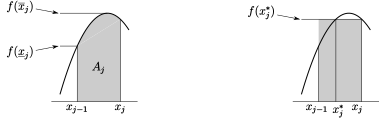
\includegraphics{rectApprox2}
         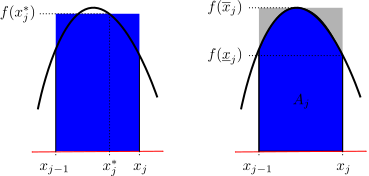
\includegraphics{rect_approx_adr3}
     \end{center}
     \end{efig}
}

We have approximated this area by $f(x_j^*)[x_j-x_{j-1}]$ (see figure left).

\item  Let $f({\overline x}_j)$ and
$f({\underline x}_j)$ be the largest and smallest values\footnote{Here we are
using the
extreme value theorem --- its proof is beyond the scope of this course. The
theorem says
that any continuous function on a closed interval must attain a minimum and
maximum at
least once. In this situation this implies that for any continuous function
$f(x)$,
there are $x_{j-1}\le {\overline x}_j, {\underline x}_j\le x_j$ such that
$f({\underline
x}_j)\le f(x) \le f({\overline x}_j)$ for all $x_{j-1}\le x\le x_j$.} of $f(x)$
for
$x_{j-1}\le x\le x_j$. Then the true area is bounded by
\begin{align*}
  f({\underline x}_j)[x_j-x_{j-1}] \leq
A_j \leq f({\overline x}_j)[x_j-x_{j-1}].
\end{align*}
(see figure right).

\item Now since $f({\underline x}_j) \leq f(x_j^*) \leq f({\overline x}_j)$, we
also know
that
\begin{align*}
  f({\underline x}_j)[x_j-x_{j-1}] \leq
f(x_j^*)[x_j-x_{j-1}] \leq f({\overline x}_j)[x_j-x_{j-1}].
\end{align*}
\item So both the true area, $A_j$, and our approximation of that area
$f(x_j^*)[x_j - x_{j-1}]$  have to lie between $f({\overline
x}_j)[x_j-x_{j-1}]$ and $f({\underline x}_j)[x_j-x_{j-1}]$. Combining these
bounds we have that the difference between the true area and our approximation
of that area is bounded by
\begin{align*}
\big|A_j-f(x_j^*)[x_j-x_{j-1}]\big|
\le[f({\overline x}_j)-f({\underline x}_j)]\cdot[x_j-x_{j-1}].
\end{align*}
(To see this think about the smallest the true area can be and the largest our
approximation can be and vice versa.)

\item Now since our function, $f(x)$ is differentiable we can apply one of the
main
theorems we learned in CLP-1 --- the Mean Value
Theorem\footnote{Recall that the mean value theorem states that for a function
continuous on $[a,b]$ and differentiable on $(a,b)$, there exists a number $c$
between
$a$ and $b$ so that
\begin{align*}
  f'(c) &= \frac{f(b)-f(a)}{b-a}.
\end{align*}
}. The MVT implies that there exists a $c$ between ${\underline
x}_j$ and ${\overline x}_j$ such that
\begin{align*}
f({\overline x}_j)-f({\underline x}_j)
=f'(c)\cdot [{\overline x}_j-{\underline x}_j]
\end{align*}
\item By the assumption that $|f'(x)|\le F$ for all $x$ and the fact that
${\underline
x}_j$ and ${\overline x}_j$ must both be between $x_{j-1}$ and $x_j$
\begin{align*}
\big|f({\overline x}_j)-f({\underline x}_j)\big|
\le F\cdot \big|{\overline x}_j-{\underline x}_j\big|
\le F\cdot [x_j-x_{j-1}]
\end{align*}
Hence the error in this part of our approximation obeys
\begin{align*}
\big|A_j-f(x_j^*)[x_j-x_{j-1}]\big|
\le F\cdot [x_j-x_{j-1}]^2.
\end{align*}
\item That was just the error in approximating $A_j$. Now we bound the total
error by
combining the errors from approximating on all the subintervals. This gives
\begin{align*}
 \left| A-\cI(\bbbp)\right|
  &= \left| \sum_{j=1}^n A_j - \sum_{j=1}^n f(x_j^*)[x_j-x_{j-1}] \right|\\
  &= \left| \sum_{j=1}^n \left(A_j - f(x_j^*)[x_j-x_{j-1}] \right) \right|
&\text{triangle inequality}\\
  &\leq \sum_{j=1}^n\left|A_j - f(x_j^*)[x_j-x_{j-1}]\right| \\
  &\leq \sum_{j=1}^n F\cdot [x_j-x_{j-1}]^2 & \text{from above}
\intertext{Now do something a little sneaky. Replace one of these factors of
$[x_j-x_{j-1}]$ (which is just the width of the $j^\mathrm{th}$ subinterval) by
the
maximum width of the subintervals:}
  &\leq \sum_{j=1}^n F\cdot M(\bbbp)\cdot [x_j-x_{j-1}]  &\text{$F$ and
$M(\bbbp)$ are
  constant}\\
  &\leq F\cdot M(\bbbp)\cdot \sum_{j=1}^n [x_j-x_{j-1}] & \text{sum is total
width}\\
  & = F\cdot M(\bbbp)\cdot (b-a).
\end{align*}
% \begin{alignat*}{3}
% \big|A-\cI(\bbbp)\big|
%      &=\bigg|A-\sum_{j=1}^nf(x_j^*)[x_j-x_{j-1}]\bigg|\,
%      &&\le\sum_{j=1}^n\Big|A_j-f(x_j^*)[x_j-x_{j-1}]\Big|\\[0.05in]
% &\le \sum_{j=1}^n F\ [x_j-x_{j-1}]^2
%      &&= \sum_{j=1}^n F\ [x_j-x_{j-1}]\ [x_j-x_{j-1}]\\[0.05in]
% &\le \sum_{j=1}^n F\ M(\bbbp)\ [x_j-x_{j-1}]
%      &&= F\ M(\bbbp)   \sum_{j=1}^n\  [x_j-x_{j-1}] \\[0.05in]
% &=F\ M(\bbbp)\ (b-a)
% \end{alignat*}
\item Since $a$, $b$ and $F$ are fixed, this tends to zero as the maximum
rectangle
width $M(\bbbp)$ tends to zero.
\end{itemize}

Thus, we have proven
\begin{theorem}
Assume that $f(x)$ is continuous for $a\le x\le b$, and
is differentiable for all $a<x<b$ with $|f'(x)|\le F$, for some
constant $F$.  Then,
as the maximum rectangle width $M(\bbbp)$ tends to zero,
$\cI(\bbbp)$ always converges to $A$, the area
between the graph of $y=f(x)$ and the $x$--axis,
with $x$ running from $a$ to $b$.
\end{theorem}

\vspace{1in}

\section{Basic Properties of the Definite Integral}
When we studied limits and derivatives, we developed methods for taking limits
or derivatives of ``complicated functions'' like $f(x)=x^2 + \sin(x)$ by
understanding how limits and derivatives interact with basic arithmetic
operations like addition and subtraction. This allowed us to reduce the problem
into one of of computing derivatives of simpler functions like $x^2$ and
$\sin(x)$. Along the way we established
simple rules such as
\begin{align*}
  \lim_{x\to a}(f(x)+g(x)) &= \lim_{x\to a}f(x) + \lim_{x\to a} g(x)
&\text{and}&&
  \diff{}{x}(f(x)+g(x)) &= \diff{f}{x} + \diff{g}{x}
\end{align*}
Some of these rules have very natural analogues for integrals and we discuss
them below. Unfortunately the analogous rules for integrals of products of
functions or integrals of compositions of functions are more complicated than
those for limits or derivatives. We discuss those rules at length in subsequent
sections. For now let us consider some of the simpler rules of the arithmetic
of
integrals.

\vspace*{\fill}

\begin{theorem}[Arithmetic of Integration]\label{thm:Intarith}
Let $a,b$ and $A,B,C$ be real numbers. Let the functions $f(x)$ and $g(x)$
be integrable on an interval that contains $a$ and $b$. Then
\begin{align*}
\text{(a)}&& \int_a^b \left( f(x) + g(x) \right)\dee{x}
&= \int_a^b f(x)\dee{x} + \int_a^b g(x)\dee{x}\\
%
\text{(b)}&&
\int_a^b\left(f(x)-g(x)\right)\dee{x}
&= \int_a^b f(x)\dee{x} - \int_a^b g(x)\dee{x}\\
%
\text{(c)}&& \int_a^b C f(x) \dee{x}
&= C\cdot \int_a^b f(x)\dee{x}
\intertext{Combining these three rules we have}
%
\text{(d)}&& \int_a^b \left( Af(x) + Bg(x) \right)\dee{x}
&= A\int_a^b f(x)\dee{x} + B\int_a^b g(x)\dee{x}
\intertext{That is, integrals depend linearly on the integrand.}
%
\text{(e)}&& \int_a^b \dee{x} = \int_a^b 1 \cdot \dee{x} &= b-a
\end{align*}
%
% \begin{align*}
% &\hskip-0.5in\text{(a)}&
% \int_a^b[f(x)+g(x)]\dee{x}&= \int_a^b f(x)\dee{x} + \int_a^b g(x)\dee{x}
% \\[0.1in]
% &\hskip-0.5in\text{(b)}&
% \int_a^b[f(x)-g(x)]\dee{x}&= \int_a^b f(x)\dee{x} - \int_a^b g(x)\dee{x}
% \\[0.1in]
% &\hskip-0.5in\text{(c)}&
% \int_a^b[C f(x)]\dee{x}&= C\int_a^b f(x)\dee{x} \\[0.1in]
% &\hskip-0.5in\text{(d)}&
% \int_a^b[Af(x)+Bg(x)]\dee{x}&= A\int_a^b f(x)\dee{x} + B\int_a^b g(x)\dee{x}
% \\
% \intertext{That is, integrals depend linearly on the integrand.}
% &\hskip-0.5in\text{(e)}&
% \int_a^b\dee{x}&= b-a
% \end{align*}
\end{theorem}
It is not too hard to prove this result from the definition of the definite
integral.
Additionally we only really need to prove (d) and (e) since
\begin{itemize}
 \item (a) follows from (d) by setting $A=B=1$,
 \item (b) follows from (d) by setting $A=1, B=-1$, and
 \item (c) follows from (d) by setting $A=C, B=0$.
\end{itemize}
\begin{proof}
As noted above, it suffices for us to prove (d) and (e). Since (e) is easier,
we
will
start with that. It is also a good warm-up for (d).
\begin{itemize}
 \item The definite integral in (e), $\int_a^b 1 \dee{x}$, can be interpreted
geometrically as the area of the rectangle with height 1 running from $x=a$ to
$x=b$; this
area is clearly $b-a$. We can also prove this formula from the definition of
the
integral
(Definition~\ref{def:INTintegral}):
\begin{align*}
\int_a^b\dee{x}
&=\lim_{n\rightarrow\infty}\sum_{i=1}^n f(x_{i,n}^*)\,\frac{b-a}{n}
&\text{by definition}\\
&=\lim_{n\rightarrow\infty}\sum_{i=1}^n 1\,\frac{b-a}{n}
&\text{since $f(x)=1$}\\
&=\lim_{n\rightarrow\infty}(b-a) \sum_{i=1}^n \frac{1}{n}
&\text{since $a,b$ are constants}\\
&=\lim_{n\rightarrow\infty}(b-a)\\
&=b-a
\end{align*}
as required.
\item To prove (d) let us start by defining $h(x) = Af(x)+Bg(x)$ and then we
need to
express the integral of $h(x)$ in terms of those of $f(x)$ and $g(x)$. We use
Definition~\ref{def:INTintegral} and some algebraic manipulations\footnote{Now
is a good
time to look back at Theorem~\ref{thm:INTsummationArith}.} to arrive at the
result.
\begin{align*}
% \int_a^b\left( Af(x) + Bg(x)\right)\dee{x}
\int_a^bh(x) \dee{x}
&= \sum_{i=1}^n h(x_{i,n}^*)\cdot\frac{b-a}{n}
&\text{by Definition~\ref{def:INTintegral}}\\
&= \sum_{i=1}^n \left(Af(x_{i,n}^*)+Bg(x_{i,n}^*) \right)\cdot \frac{b-a}{n}\\
&= \sum_{i=1}^n \left(Af(x_{i,n}^*)\cdot \frac{b-a}{n} + Bg(x_{i,n}^*)\cdot
\frac{b-a}{n}
\right)\\
&= \left(\sum_{i=1}^n Af(x_{i,n}^*)\cdot \frac{b-a}{n}\right)
 + \left(\sum_{i=1}^n Bg(x_{i,n}^*)\cdot \frac{b-a}{n}\right)
&\text{by Theorem~\ref{thm:INTsummationArith}(b)}\\
&= A\left(\sum_{i=1}^n f(x_{i,n}^*)\cdot \frac{b-a}{n}\right)
 + B\left(\sum_{i=1}^n g(x_{i,n}^*)\cdot \frac{b-a}{n}\right)
&\text{by Theorem~\ref{thm:INTsummationArith}(a)}\\
&= A \int_a^b f(x) \dee{x} + B \int_a^b g(x) \dee{x}
&\text{by Definition~\ref{def:INTintegral}}
\end{align*}
as required.
\end{itemize}
\end{proof}
Using this Theorem we can integrate sums, differences and constant multiples of
functions
we know how to integrate. For example:
\begin{eg}
In Example~\ref{eg:INTexparea} we saw that $\int_0^1 e^x\dee{x}=e-1$. So
\begin{align*}
\int_0^1\big(e^x+7\big)\dee{x}
&= \int_0^1 e^x\dee{x} + 7\int_0^1 1 \dee{x} \\
&\hspace{3cm}\text{by Theorem~\ref{thm:Intarith}(d) with
$A=1,f(x)=e^x,B=7,g(x)=1$} \\
&=(e-1)+7\times (1-0) \\
&\hspace{3cm}\text{by Example~\ref{eg:INTexparea} and
Theorem~\ref{thm:Intarith}(e)} \\
&=e+6
\end{align*}
\end{eg}

When we gave the formal definition of $\int_a^b f(x) \dee{x}$ in
Definition~\ref{def:INTintegral} we explained that the integral could be
interpreted as the signed area between the curve $y=f(x)$ and the $x$-axis on
the interval $[a,b]$. In order for this interpretation to make sense we
required
that $a<b$, and though we remarked that the integral makes sense when $a>b$ we
did not explain any further. Thankfully there is an easy way to express the
integral $\int_a^b f(x)\dee{x}$ in terms of $\int_b^a f(x)\dee{x}$ --- making
it
always possible to write an integral so the lower limit of integration
is less than the upper limit of integration. Theorem~\ref{thm:Intdomain},
below,
tell us that, for example, $\int_7^3 e^x\dee{x} = - \int_3^7 e^x\dee{x}$. The same
theorem also provides us with two other simple manipulations of the limits of
integration.
\begin{theorem}[Arithmetic for the Domain of Integration]\label{thm:Intdomain}
Let $a,b,c$  be real numbers. Let the function $f(x)$
be integrable on an interval that contains $a$, $b$ and $c$. Then
\begin{align*}
\text{(a)}&&
\int_a^a f(x)\dee{x}&= 0\\
\text{(b)}&&
\int_b^a f(x)\dee{x}&= -\int_a^b f(x)\dee{x} \\
\text{(c)}&&
\int_a^b f(x)\dee{x}&= \int_a^c f(x)\dee{x} + \int_c^b f(x)\dee{x}
\end{align*}
\end{theorem}
The proof of this statement is not too difficult.
\begin{proof}
Let us prove the statements in order.
\begin{itemize}
 \item Consider the definition of the definite integral
\begin{align*}
  \int_a^b f(x) \dee{x} &= \lim_{n \to \infty} \sum_{i=1}^n
f(x_{i,n}^*)\cdot\frac{b-a}{n}
\end{align*}
If we now substitute $b=a$ in this expression we have
\begin{align*}
  \int_a^a f(x) \dee{x}
  &= \lim_{n \to \infty} \sum_{i=1}^n
f(x_{i,n}^*)\cdot\underbrace{\frac{a-a}{n}}_{=0}\\
  &= \lim_{n \to \infty} \sum_{i=1}^n \underbrace{f(x_{i,n}^*)\cdot 0}_{=0}\\
  &= \lim_{n \to \infty} 0 \\
  &= 0
\end{align*}
as required.
% \item Consider now the definite integral $\int_A^B f(x) \dee{x}$. Shortly we
% will
% substitute $A=b$ and $B=a$, but first lets write down the definition of this
% integral using Definition~\ref{def:INTintegral}.
% \begin{align*}
% \int_A^B f(x) \dee{x}
% &=\lim_{n \to \infty} \sum_{i=1}^n f(x_{i,n}^*)\cdot\frac{B-A}{n}
% \intertext{Now substitute $A=b$ and $B=a$ into this expression:}\\
% \int_b^a f(x) \dee{x}
% &=\lim_{n \to \infty} \sum_{i=1}^n f(x_{i,n}^*)\cdot\frac{a-b}{n}\\
% &=\lim_{n \to \infty} \sum_{i=1}^n f(x_{i,n}^*)\cdot (-1) \cdot
% \frac{b-a}{n}\\
% &=\lim_{n \to \infty} (-1)\cdot \sum_{i=1}^n f(x_{i,n}^*)\cdot\frac{b-a}{n}
% &\text{by Theorem~\ref{thm:INTsummationArith}(a)}\\
% &=(-1)\lim_{n \to \infty} \sum_{i=1}^n f(x_{i,n}^*)\cdot\frac{b-a}{n}
% &\text{by arithmetic of limits}\\
% &= (-1)\cdot \int_a^b f(x) \dee{x}
% &\text{by Definition~\ref{def:INTintegral}}
% \end{align*}
% as required.

\item Consider now the definite integral $\int_a^b f(x) \dee{x}$. We will sneak
up on the proof by first examining Riemann sum approximations to both this and
$\int_b^a f(x)\dee{x}$. The midpoint Riemann sum approximation to $\int_a^b
f(x)\dee{x}$ with $4$ subintervals (so that each subinterval has width
$\frac{b-a}{4}$)
is
\begin{align*}
&\left\{f\Big(a+\frac{1}{2}\frac{b-a}{4}\Big)
      +f\Big(a+\frac{3}{2}\frac{b-a}{4}\Big)
      +f\Big(a+\frac{5}{2}\frac{b-a}{4}\Big)
  + f\Big(a+\frac{7}{2}\frac{b-a}{4}\Big)
  \right\}\cdot\frac{b-a}{4}\\
&=\left\{f\Big(\frac{7}{8}a+\frac{1}{8}b\Big)
   +f\Big(\frac{5}{8}a+\frac{3}{8}b\Big)
   +f\Big(\frac{3}{8}a+\frac{5}{8}b\Big)
   +f\Big(\frac{1}{8}a+\frac{7}{8}b\Big)\right\}\cdot\frac{b-a}{4}
\end{align*}
Now we do the same for $\int_b^a f(x)\dee{x}$ with $4$ subintervals. Note that $b$
is now the lower limit on the integral and $a$ is now the upper limit on the
integral. This is likely to cause confusion when we write out the Riemann sum,
so we'll temporarily rename $b$ to $A$ and $a$ to $B$. The midpoint Riemann sum
approximation to $\int_A^B f(x)\dee{x}$ with $4$ subintervals is
\begin{align*}
&\left\{f\Big(A+\frac{1}{2}\frac{B-A}{4}\Big)
      +f\Big(A+\frac{3}{2}\frac{B-A}{4}\Big)
      +f\Big(A+\frac{5}{2}\frac{B-A}{4}\Big)
   +f\Big(A+\frac{7}{2}\frac{B-A}{4}\Big)\right\}\cdot \frac{B-A}{4}\\
&=\left\{f\Big(\frac{7}{8}A+\frac{1}{8}B\Big)
   +f\Big(\frac{5}{8}A+\frac{3}{8}B\Big)
   +f\Big(\frac{3}{8}A+\frac{5}{8}B\Big)
   +f\Big(\frac{1}{8}A+\frac{7}{8}B\Big)\right\}\cdot \frac{B-A}{4}
\intertext{Now recalling that $A=b$ and $B=a$, we have that the midpoint
Riemann sum approximation to $\int_b^a f(x)\dee{x}$ with  $4$ subintervals is}
&\left\{f\Big(\frac{7}{8}b+\frac{1}{8}a\Big)
   +f\Big(\frac{5}{8}b+\frac{3}{8}a\Big)
   +f\Big(\frac{3}{8}b+\frac{5}{8}a\Big)
   +f\Big(\frac{1}{8}b+\frac{7}{8}a\Big)\right\}\cdot \frac{a-b}{4}
\end{align*}
Thus we see that the Riemann sums for the two integrals are nearly identical
--- the only difference being the factor of $\frac{b-a}{4}$ versus
$\frac{a-b}{4}$. Hence the two Riemann sums are negatives of each other.

The same computation with $n$ subintervals shows that the midpoint Riemann sum
approximations to $\int_b^a f(x)\dee{x}$ and $\int_a^b f(x)\dee{x}$ with $n$
subintervals are negatives of each other. Taking the limit $n\rightarrow\infty$
gives $\int_b^a f(x)\dee{x}= -\int_a^b f(x)\dee{x}$.


\item Finally consider (c) --- we will not give a formal proof of this, but
instead will interpret it geometrically. Indeed one can also interpret (a)
geometrically. In both cases these become statements about areas:
\begin{align*}
\int_a^a f(x)\dee{x}=0\qquad\text{and}\qquad
\int_a^b f(x)\dee{x}= \int_a^c f(x)\dee{x} + \int_c^b f(x)\dee{x}
\end{align*}
are
\begin{align*}
\text{Area}\big\{\ (x,y)\ \big|\ a\le x\le a,\ 0\le y\le f(x)\ \big\}=0
\end{align*}
and
\begin{align*}
\text{Area}\big\{\ (x,y)\ \big|\ a\le x\le b,\ 0\le y\le f(x)\ \big\}
&=\text{Area}\big\{\ (x,y)\ \big|\ a\le x\le c,\ 0\le y\le f(x)\ \big\} \\
&\hskip0.5in
+\text{Area}\big\{\ (x,y)\ \big|\ c\le x\le b,\ 0\le y\le f(x)\ \big\}
\end{align*}
respectively. Both of these geometric statements
are intuitively obvious. See the figures below.
\begin{wfig}
\begin{center}
  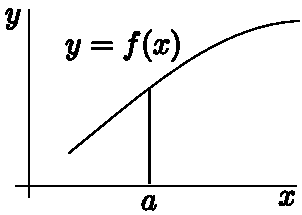
\includegraphics{areaAA}\qquad\qquad
  \raisebox{-0.05\height}{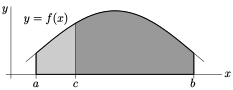
\includegraphics{areaABC}}
\end{center}
\end{wfig}
Note that we have assumed that $a\leq c \leq b$ and that $f(x)\geq 0$. One can
remove
these restrictions and also make the proof more formal, but it becomes quite
tedious and
less intuitive.
\end{itemize}
\end{proof}
\begin{remark}
For notational simplicity, let's assume that $a\le c\le b$ and $f(x)\ge 0$
for all $a\le x\le b$.
The geometric interpretations of the identities
\begin{align*}
\int_a^a f(x)\dee{x}=0\qquad\text{and}\qquad
\int_a^b f(x)\dee{x}= \int_a^c f(x)\dee{x} + \int_c^b f(x)\dee{x}
\end{align*}
are
\begin{align*}
\text{Area}\big\{\ (x,y)\ \big|\ a\le x\le a,\ 0\le y\le f(x)\ \big\}=0
\end{align*}
and
\begin{align*}
\text{Area}\big\{\ (x,y)\ \big|\ a\le x\le b,\ 0\le y\le f(x)\ \big\}
&=\text{Area}\big\{\ (x,y)\ \big|\ a\le x\le c,\ 0\le y\le f(x)\ \big\} \\
&\hskip0.5in
+\text{Area}\big\{\ (x,y)\ \big|\ c\le x\le b,\ 0\le y\le f(x)\ \big\}
\end{align*}
respectively. Both of these geometric statements
are intuitively obvious. See the figures below.
\begin{wfig}
\begin{center}
  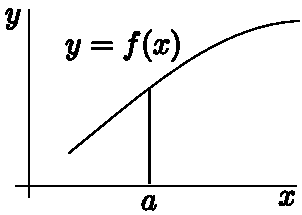
\includegraphics{areaAA}\qquad\qquad
  \raisebox{-0.05\height}{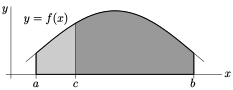
\includegraphics{areaABC}}
\end{center}
\end{wfig}
\end{remark}


\begin{eg}\label{eg:INTPROPxa}
Back in Example~\ref{eg:INTtriangle} we saw that when $b>0$
$\int_0^b x\dee{x} =\frac{b^2}{2}$. We'll now verify that
$\int_0^b x\dee{x} =\frac{b^2}{2}$ is still true when $b=0$ and
also when $b<0$.
\begin{itemize}
\item First consider $b=0$. Then the statement $\int_0^b x\dee{x}
=\frac{b^2}{2}$ becomes
\begin{align*}
\int_0^0 x\dee{x} =0
\end{align*}
This is an immediate consequence of Theorem \ref{thm:Intdomain}(a).
\item Now consider $b<0$. Let us write $B=-b$, so that $B>0$. In
Example~\ref{eg:INTtriangle} we saw that
\begin{align*}
\int_{-B}^0 x\dee{x} =-\frac{B^2}{2}.
\end{align*}
So we have
\begin{align*}
\int_0^b x\dee{x}
&=\int^{-B}_0 x\dee{x} =- \int_{-B}^0 x\dee{x} & \text{by
Theorem~\ref{thm:Intdomain}(b)}\\
& =-\left(-\frac{B^2}{2}\right) & \text{by Example~\ref{eg:INTtriangle}}\\
& =\frac{B^2}{2} = \frac{b^2}{2}
\end{align*}
\end{itemize}
We have now shown that
\begin{align*}
\int_0^b x\dee{x} &=\frac{b^2}{2} &\text{ for all real numbers $b$}
\end{align*}
\end{eg}

\begin{eg}\label{eg:INTPROPx}
Applying Theorem \ref{thm:Intdomain} yet again, we have, for
all real numbers $a$ and $b$,
\begin{align*}
\int_a^b x\dee{x} &=  \int_a^0 x\dee{x} + \int_0^b x\dee{x} &
           \text{by Theorem \ref{thm:Intdomain}(c) with $c=0$}\\
               &=  \int_0^b x\dee{x} - \int_0^a x\dee{x} &
            \text{by Theorem \ref{thm:Intdomain}(b)}\\
               &=\frac{b^2-a^2}{2} &
            \text{by Example \ref{eg:INTPROPxa}, twice}
\end{align*}
We can also understand this result geometrically.
\begin{wfig}
 \begin{center}
  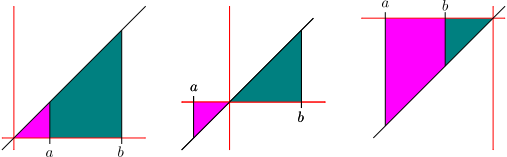
\includegraphics[height=4cm]{triangles_adr}
 \end{center}
\end{wfig}
\begin{itemize}
 \item (left) When $0<a<b$, the integral represents the area in green which
is the difference of two right--angle triangles --- the larger with area $b^2/2$
and the smaller with area $a^2/2$.
\item (centre) When $a<0<b$, the integral represents the signed area of the two
displayed triangles. The one above the axis has area $b^2/2$ while the one
below has area $-a^2/2$ (since it is below the axis).
\item (right) When $a<b<0$, the integral represents the signed area in purple
of the difference between the two triangles --- the larger with area $-a^2/2$
and the smaller with area $-b^2/2$.
\end{itemize}

\end{eg}


Theorem~\ref{thm:Intdomain}(c) shows us how we can split an integral over a
larger interval into one over two (or more) smaller intervals. This is
particularly useful for dealing with piece-wise functions, like $|x|$.
\begin{eg}\label{eg:INTPROPabs}
Using Theorem~\ref{thm:Intdomain}, we can readily evaluate integrals involving
$|x|$. First, recall that
\begin{align*}
|x|=\begin{cases}
          x & \text{if $x\ge 0$} \\
         -x & \text{if $x< 0$}
    \end{cases}
\end{align*}
Now consider (for example) $\int_{-2}^3 |x| \dee{x}$. Since the integrand
changes at $x=0$, it makes sense to split the interval of integration at that
point:
\begin{align*}
  \int_{-2}^3 |x| \dee{x}
&= \int_{-2}^0 |x| \dee{x} + \int_0^3 |x| \dee{x}
&\text{by Theorem~\ref{thm:Intdomain}}\\
&= \int_{-2}^0 (-x) \dee{x} + \int_0^3 x \dee{x}
&\text{by definition of $|x|$}\\
&= -\int_{-2}^0 x\dee{x} + \int_0^3 x \dee{x}
&\text{by Theorem~\ref{thm:Intarith}(c)}\\
&= - (-2^2/2) + (3^2/2) = (4+9)/2\\
&= 13/2
\end{align*}
We can go further still --- given a function $f(x)$ we can rewrite
the integral of $f(|x|)$ in terms of the integral of $f(x)$ and $f(-x)$.
\begin{align*}
\int_{-1}^1 f\big(|x|\big)\dee{x}
& = \int_{-1}^0 f\big(|x|\big)\dee{x}+ \int_0^1 f\big(|x|\big)\dee{x} \\
& = \int_{-1}^0 f(-x)\dee{x}+ \int_0^1 f(x)\dee{x}
\end{align*}
\end{eg}

Here is a more concrete example.
\begin{eg}
Let us compute $\int_{-1}^1 \big(1-|x|\big)\dee{x}$ again. In
Example~\ref{eg:INTtriangleB} we evaluated this integral by interpreting it as
the area of a triangle. This time we are going to use \emph {only} the
properties given in Theorems~\ref{thm:Intarith} and~\ref{thm:Intdomain} and the
facts that
\begin{align*}
\int_a^b \dee{x} &= b-a &\text{and}&&
\int_a^b x\dee{x}=\frac{b^2-a^2}{2}
\end{align*}
That $\int_a^b\dee{x} = b-a$ is part (e) of Theorem~\ref{thm:Intarith}.
We saw that $\int_a^b x\dee{x}=\frac{b^2-a^2}{2}$ in Example~\ref{eg:INTPROPx}.


First we are going to get rid of the absolute value signs by splitting the
interval over which we integrate. Recalling that $|x|=x$ whenever $x\ge 0$ and
$|x|=-x$ whenever $x\le 0$, we split the interval by
Theorem~\ref{thm:Intdomain}(c),
\begin{align*}
\int_{-1}^1 \big(1-|x|\big)\dee{x}
&=\int_{-1}^0 \big(1-|x|\big)\dee{x}
   + \int_0^1 \big(1-|x|\big)\dee{x} \\
&=\int_{-1}^0 \big(1-(-x)\big)\dee{x}
   + \int_0^1 \big(1-x\big)\dee{x} \\
&=\int_{-1}^0 \big(1+x\big)\dee{x}
   + \int_0^1 \big(1-x\big)\dee{x}
\end{align*}
Now we apply parts (a) and (b) of Theorem \ref{thm:Intarith}, and then
\begin{align*}
\int_{-1}^1 \big[1-|x|\big]\dee{x}
&=\int_{-1}^0 1\dee{x}
  + \int_{-1}^0 x\dee{x}
   + \int_0^1 1\dee{x}
   - \int_0^1 x\dee{x} \\[0.1in]
&=[0-(-1)]+\frac{0^2-(-1)^2}{2}+[1-0]-\frac{1^2-0^2}{2} \\
&=1
\end{align*}
\end{eg}

\subsection{More Properties of Integration: Even and Odd Functions}
\label{sec:evenodd}
Recall\footnote{We haven't done this in this course, but you should have seen
it in your differential calculus course or perhaps even earlier.} the following
definition
\begin{defn}\label{def:INTevenodd}
  Let $f(x)$ be a function. Then,
 \begin{itemize}
  \item we say that $f(x)$ is even when $f(x)=f(-x)$ for all $x$, and
  \item we say that $f(x)$ is odd when $f(x)=-f(-x)$ for all $x$.
 \end{itemize}
\end{defn}
Of course most functions are neither even nor odd, but many of the standard
functions you know are.
\begin{eg}[Even functions]\label{eg:lefthalfevenfunction}
\begin{itemize}
   \item Three examples of even functions are $f(x)=|x|$, $f(x)=\cos x$ and
  $f(x)=x^2$. In fact, if $f(x)$ is any even power of $x$, then $f(x)$ is an
even function.
   \item The part of the graph $y=f(x)$ with $x\le 0$, may be constructed by
         drawing the part of the graph with $x\ge 0$ (as in the figure
         on the left below) and then reflecting it in the $y$--axis
         (as in the figure on the right below).
        \begin{efig}
        \begin{center}
            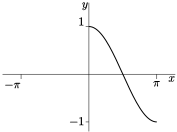
\includegraphics[scale=0.9]{evenCosPt}\qquad
            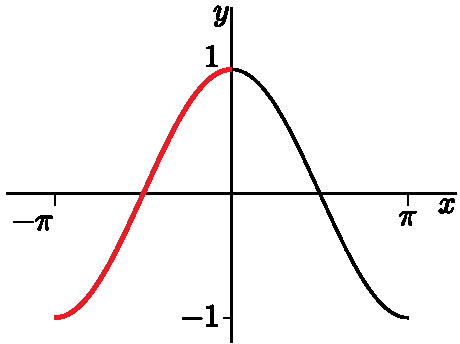
\includegraphics[scale=0.9]{evenCos}
         \end{center}
         \end{efig}
  \item In particular, if $f(x)$ is an even function and $a>0$, then
      the two sets
   \begin{align*}
     &\big\{\ (x,y)\ \big|\
       \text{$0\le x\le a$ and $y$ is between $0$ and $f(x)$} \ \big\} \\
     &\big\{\ (x,y)\ \big|\
       \text{$-a\le x\le 0$ and $y$ is between $0$ and $f(x)$} \ \big\}
    \end{align*}
   are reflections of each other in the $y$--axis and so have the same
   signed area. That is
  \begin{align*}
        \int_0^a f(x)\dee{x} &= \int_{-a}^0 f(x)\dee{x}
  \end{align*}
   \end{itemize}
\end{eg}
\begin{eg}[Odd functions]\label{eg:areaunderoddfunction}
   \begin{itemize}
   \item Three examples of odd functions are $f(x)=\sin x$, $f(x)=\tan x$ and
  $f(x)=x^3$. In fact, if $f(x)$ is any odd power of $x$, then $f(x)$ is
         an odd function.
   \item The part of the graph $y=f(x)$ with $x\le 0$, may be constructed by
drawing the part of the graph with $x\ge 0$ (like the solid line in the figure
on the left below) and then reflecting it in the $y$--axis (like the dashed
line
in the figure on the left below) and then reflecting the result in the $x$--axis
(i.e. flipping it upside down, like in the figure on the right, below).
        \begin{efig}
        \begin{center}
            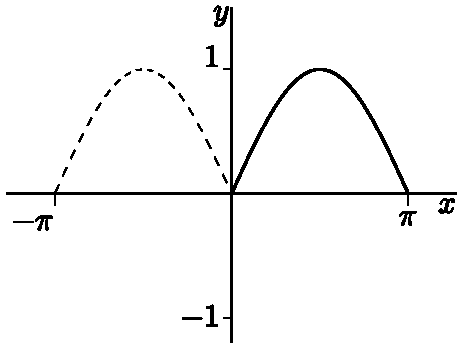
\includegraphics[scale=0.9]{oddSinPt}\qquad
            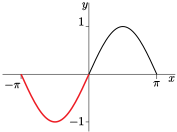
\includegraphics[scale=0.9]{oddSin}
         \end{center}
         \end{efig}
\item In particular, if $f(x)$ is an odd function and $a>0$, then the
    signed areas of the two sets
   \begin{align*}
     &\big\{\ (x,y)\ \big|\
       \text{$0\le x\le a$ and $y$ is between $0$ and $f(x)$} \ \big\} \\
     &\big\{\ (x,y)\ \big|\
       \text{$-a\le x\le 0$ and $y$ is between $0$ and $f(x)$} \ \big\}
    \end{align*}
      are negatives of each other --- to get from the first set to the second
set, you flip it upside down, in addition to reflecting it in the $y$--axis.
That is
  \begin{align*}
        \int_0^a f(x)\dee{x} = -\int_{-a}^0 f(x)\dee{x}
  \end{align*}
   \end{itemize}
\end{eg}

We can exploit the symmetries noted in the examples above, namely
\begin{align*}
        \int_0^a f(x)\dee{x} &= \int_{-a}^0 f(x)\dee{x} & \text{for $f$ even}\\
        \int_0^a f(x)\dee{x} &= -\int_{-a}^0 f(x)\dee{x} & \text{for $f$ odd}
\intertext{together with Theorem~\ref{thm:Intdomain}}
  \int_{-a}^a f(x)\dee{x} &= \int_{-a}^0 f(x)\dee{x} + \int_0^a f(x) \dee{x}
\end{align*}
in order to simplify the integration of even and odd functions over intervals
of the form $[-a,a]$.
\begin{theorem}[Even and Odd]\label{thm:INTevenodd}
Let $a>0$.
\begin{enumerate}[(a)]
\item If $f(x)$ is an even function, then
\begin{align*}
\int_{-a}^a f(x) \dee{x} = 2\int_0^a f(x) \dee{x}
\end{align*}
\item If $f(x)$ is an odd function, then
\begin{align*}
\int_{-a}^a f(x) \dee{x} = 0
\end{align*}
\end{enumerate}
\end{theorem}
\begin{proof}
For any function
\begin{align*}
\int_{-a}^a f(x)\dee{x} = \int_0^a f(x)\dee{x} + \int_{-a}^0 f(x)\dee{x}
\end{align*}
When $f$ is even, the two terms on the right hand side are equal.
When $f$ is odd, the two terms on the right hand side are negatives of
each other.
\end{proof}

\newpage %there was weird spacing
\subsection{Optional --- More Properties of Integration: Inequalities for
Integrals}

We are still unable to integrate many functions, however with a little work we
can infer bounds on integrals from bounds on their integrands.
\begin{theorem}[Inequalities for Integrals]\label{thm:INTineq}
Let $a\le b$  be real numbers and let the functions $f(x)$ and $g(x)$
be integrable on the interval $a\le x\le b$.
\begin{enumerate}[(a)]
\item If $f(x)\ge 0$ for all $a\le x\le b$, then
\begin{align*}
\int_a^b f(x)\,\dee{x} \ge 0
\end{align*}
\item If $f(x)\le g(x)$ for all $a\le x\le b$, then
\begin{align*}
\int_a^b f(x)\,\dee{x} \le \int_a^b g(x)\,\dee{x}
\end{align*}
\item If there are constants $m$ and $M$ such that  $m\le f(x)\le M$
for all $a\le x\le b$, then
\begin{align*}
m(b-a)\le \int_a^b f(x)\,\dee{x} \le M(b-a)
\end{align*}
\item We have
\begin{align*}
\bigg|\int_a^b f(x)\,\dee{x}\bigg|\le \int_a^b |f(x)|\,\dee{x}
\end{align*}
\end{enumerate}
\end{theorem}

\begin{proof}
\begin{enumerate}[(a)]
 \item By interpreting the integral as the signed area, this statement
simply says that if the curve $y=f(x)$ lies above the
$x$--axis and $a\le b$, then the signed area of the set
$\big\{\ (x,y)\ \big|\ a\le x\le b,\   0\le y\le f(x)\ \big\}$
is at least zero. This is quite clear. Alternatively, we could argue more
algebraically from Definition~\ref{def:INTintegral}. We observe that when we
define $\int_a^b f(x)\dee{x}$ via Riemann sums, every
summand, $f(x_{i,n}^*)\,\frac{b-a}{n}\ge 0$. Thus the whole sum is nonnegative
and consequently, so is the limit, and thus so is the integral.

\item We are assuming that $g(x)-f(x)\geq 0$, so part (a) gives
\begin{align*}
\int_a^b\big[g(x)-f(x)\big]\dee{x}\ge 0
&\implies \int_a^b g(x)\,\dee{x}-\int_a^b f(x)\,\dee{x}\ge 0 \\
&\implies \int_a^b f(x)\,\dee{x} \le \int_a^b g(x)\,\dee{x}
\end{align*}

\item Applying part (b) with $g(x)=M$ for all $a\le x\le b$ gives
\begin{align*}
\int_a^b f(x)\,\dee{x} \le \int_a^b M\,\dee{x} = M(b-a)
\end{align*}
Similarly, viewing $m$ as a (constant) function, and applying part (b) 
gives
\begin{align*}
m\le f(x) \implies \overbrace{\int_a^bm\,\dee{x}}^{=m(b-a)} \le 
\int_a^b f(x)\,\dee{x}
\end{align*}


\item  For any $x$, $|f(x)|$ is either $f(x)$ or $-f(x)$ (depending on whether
$f(x)$ is positive or negative), so we certainly have
\begin{align*}
f(x)&\le |f(x)| & \text{and}&&
-f(x)&\le |f(x)|
\end{align*}
Applying part (c) to each of those inequalities gives
\begin{align*}
\int_a^b f(x)\,\dee{x} &\le \int_a^b |f(x)|\,\dee{x} & \text{and} &&
-\int_a^b f(x)\,\dee{x} &\le \int_a^b |f(x)|\,\dee{x}
\end{align*}
Now $\Big|\int_a^b f(x)\,\dee{x}\Big|$ is either equal to $\int_a^b f(x)\,\dee{x}$ or
$-\int_a^b f(x)\,\dee{x}$ (depending on whether the integral is positive or
negative). In either case we can apply the above two inequalities to get the
same result, namely
\begin{align*}
  \left|\int_a^b f(x)\,\dee{x}\right| &\leq \int_a^b |f(x)|\,\dee{x}.
\end{align*}
\end{enumerate}
\end{proof}

\begin{eg}[$\int_0^{\nicefrac{\pi}{3}}\sqrt{\cos x}\dee{x}$]
Consider the integral
\begin{align*}
\int_0^{\nicefrac{\pi}{3}}\sqrt{\cos x}\dee{x}
\end{align*}
This is not so easy to compute exactly\footnote{It is not too hard to use
Riemann sums and a computer to evaluate it numerically: $0.948025319\dots$.},
but we can bound it quite quickly.

For $x$ between $0$ and $\frac{\pi}{3}$, the function $\cos x$ takes
values\footnote{You know the graphs of sine and cosine, so you should be
able to work this out without too much difficulty.}
between $1$ and $\frac{1}{2}$. Thus the function $\sqrt{\cos x}$ takes
values between $1$ and $\frac{1}{\sqrt{2}}$. That is
\begin{align*}
 \frac{1}{\sqrt{2}} &\le \sqrt{\cos x} \le 1
& \text{for $0\le x\le \frac{\pi}{3}$}.
\end{align*}
Consequently, by Theorem \ref{thm:INTineq}(c) with
$a=0$, $b=\frac{\pi}{3}$, $m= \frac{1}{\sqrt{2}}$ and $M=1$,
\begin{align*}
\frac{\pi}{3\sqrt{2}} &\le \int_0^{\nicefrac{\pi}{3}} \sqrt{\cos x}\dee{x}
            \le \frac{\pi}{3}\\
\intertext{Plugging these expressions into a calculator gives us}
0.7404804898 & \le \int_0^{\nicefrac{\pi}{3}} \sqrt{\cos x}\dee{x}
\leq 1.047197551
\end{align*}
\end{eg}


\section{The Fundamental Theorem of Calculus}\label{sec fundamental}
We have spent quite a few pages (and lectures) talking about definite
integrals, what they are (Definition~\ref{def:INTintegral}), when they
exist (Theorem~\ref{thm:integrable}), how to compute some special
cases (Section~\ref{ssec knownareas}), some ways to manipulate them
(Theorem~\ref{thm:Intarith} and~\ref{thm:Intdomain}) and how to bound them
(Theorem~\ref{thm:INTineq}). Conspicuously missing from all of this has been a
discussion of how to compute them in general. It is high time we rectified
that.

The single most important tool used to evaluate integrals is called
``the fundamental theorem of calculus''. Its grand name is justified --- it
links the two branches of calculus by connecting derivatives to integrals. In
so
doing it also tells us how to compute integrals. Very roughly speaking the
derivative of an integral is the original function. This fact allows us to
compute integrals using antiderivatives\footnote{You learned these near the
end of your differential calculus course. Now is a good time to revise ---
but we'll go over them here since they are so important in what follows.}. Of
course ``very rough'' is not enough --- let's be precise.
%%
\begin{theorem}[Fundamental Theorem of Calculus]\label{thm:INTfundthmofcalc}
Let $a<b$ and let $f(x)$ be a function which is defined and continuous on
$[a,b]$.
\begin{enumerate}[\itshape {Part} 1:]
 \item Let $\ds F(x)=\int_a^x f(t)\dee{t}$ for any $x
\in[a,b]$. Then the function $F(x)$ is differentiable and further
\begin{align*}
 F'(x) &=f(x)
\end{align*}

\item Let $G(x)$ be any function which is defined and
continuous on $[a,b]$. Further let $G(x)$ be differentiable with $G'(x)=f(x)$
for all $a<x<b$. Then
\begin{align*}
\int_a^b f(x)\dee{x} &=G(b)-G(a) & \text{or equivalently} &&
\int_a^b G'(x)\dee{x} &=G(b)-G(a)
\end{align*}
\end{enumerate}
\end{theorem}

Before we prove this theorem and look at a bunch of examples of its
application, it is important that we recall one definition from differential
calculus --- antiderivatives. If $F'(x) = f(x)$ on some interval, then  $F(x)$
is called an antiderivative of $f(x)$ on that interval. So Part 2 of the
fundamental theorem of calculus tells us how to evaluate the definite integral
of $f(x)$ in terms of any of its antiderivatives ---  if  $G(x)$ is any
antiderivative of $f(x)$ then
\begin{align*}
\int_a^b f(x) \dee x &= G(b)-G(a)
\end{align*}
The form $\int_a^b G'(x)\,\dee{x} = G(b) - G(a)$ of the fundamental theorem relates the
rate of change of $G(x)$ over the interval $a\le x\le b$ to the net change of $G$ between
$x=a$ and $x=b$. For that reason, it is sometimes called the ``net change theorem''.

We'll start with a simple example. Then we'll see why the
fundamental theorem is true and then we'll do many more, and more involved,
examples.
\begin{eg}[A first example]\label{eg first}
 Consider the integral $\int_a^b x \dee{x}$ which we have explored previously
in Example~\ref{eg:INTPROPx}.
\begin{itemize}
 \item The integrand is $f(x)=x$.
 \item We can readily verify that $G(x) = \frac{x^2}{2}$ satisfies $G'(x)=f(x)$
and so is an antiderivative of the integrand.
\item Part 2 of Theorem~\ref{thm:INTfundthmofcalc} then tells us that
\begin{align*}
  \int_a^b f(x) \dee{x} &= G(b)-G(a) \\
  \int_a^b x \dee{x} &= \frac{b^2}{2} - \frac{a^2}{2}
\end{align*}
which is precisely the result we obtained (with more work) in
Example~\ref{eg:INTPROPx}.
\end{itemize}
\end{eg}


We do not give completely rigorous proofs of the two parts of the theorem ---
that is not really needed for this course. We just give the main ideas of the
proofs so that you can understand why the theorem is true.
\begin{proof}[Part 1] We wish to show that if
\begin{align*}
  F(x) &= \int_a^x f(t) \dee{t} & \text{then}&&
  F'(x) &= f(x)
\end{align*}
\begin{itemize}
 \item Assume that $F$ is the above integral and then consider $F'(x)$. By
  definition
  \begin{align*}
  F'(x) &=\lim_{h\rightarrow 0} \frac{F(x+h)-F(x)}{h}
  \end{align*}

\item To understand this limit, we interpret the terms $F(x), F(x+h)$ as signed
areas. To simplify this further, let's only consider the case that $f$ is always
nonnegative and that $h>0$. These restrictions are not hard to remove, but the
proof ideas are a bit cleaner if we keep them in place. Then we have
\begin{align*}
F(x+h)&=\text{the area of the region $\big\{\ (t,y)\ \big|\ a\le t\le x+h,\
                0\le y\le f(t)\ \big\}$} \\
F(x)&=\text{the area of the region $\big\{\ (t,y)\ \big|\ a\le t\le x,
                  \phantom{+h\ \,}\
                                             0\le y\le f(t)\ \big\}$}
\end{align*}

\item Then the numerator
\begin{align*}
F(x+h)-F(x)=\text{the area of the region $\big\{\ (t,y)\ \big|\ x\le t\le x+h,\
                0\le y\le f(t)\ \big\}$}
\end{align*}
This is just the more darkly shaded region in the figure
\begin{efig}
\begin{center}
    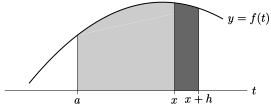
\includegraphics{fundThm}
\end{center}
\end{efig}

\item We will be taking the limit $h\rightarrow 0$. So suppose that $h$ is
very small. Then, as $t$ runs from $x$ to $x+h$, $f(t)$ runs only over
a very narrow range of values\footnote{Notice that if $f$ were
discontinuous, then this might be false.}, all close to $f(x)$.

\item So the darkly shaded region is almost a rectangle of width $h$ and height
$f(x)$ and so has an area which is very close to $f(x)h$. Thus
$\frac{F(x+h)-F(x)}{h}$ is very close to $f(x)$.
\item In the limit $h\rightarrow 0$, $\frac{F(x+h)-F(x)}{h}$ becomes
exactly $f(x)$, which is precisely what we want.
\end{itemize}
\end{proof}


\begin{proof}[Part 2]
We want to show that $\int_a^b f(t)\dee{t}=G(b)-G(a)$. To do this we exploit
the fact that the derivative of a constant is zero.
\begin{itemize}
\item Let
\begin{align*}
  H(x) &= \int_a^x f(t)\dee{t} -G(x)+G(a)
\end{align*}
Then the result we wish to prove is that $H(b)=0$.  We will do this by showing
that $H(x)=0$ for all $x$ between $a$ and $b$.

\item We first show that $H(x)$ is constant by computing its derivative:
\begin{align*}
  H'(x) &= \diff{}{x}\int_a^x f(t)\dee{t} - \diff{}{x}\left( G(x) \right)+
\diff{}{x}\left( G(a) \right)
\intertext{Since $G(a)$ is a constant, its derivative is $0$ and by assumption
the derivative of $G(x)$ is just $f(x)$, so}
  &= \diff{}{x}\int_a^x f(t)\dee{t} - f(x)
\intertext{Now Part~1 of the theorem tells us that this derivative is just
$f(x)$, so}
  &= f(x) - f(x) = 0
\end{align*}
Hence $H$ is constant.
\item To determine which constant we just compute $H(a)$:
\begin{align*}
  H(a) &= \int_a^a f(t)\dee{t} - G(a)+G(a) \\
  &= \int_a^a f(t)\dee{t} & \text{by Theorem~\ref{thm:Intdomain}(a)}\\
  &=0
\end{align*}
as required.
\end{itemize}
\end{proof}

The simple example we did above (Example~\ref{eg first}), demonstrates the
application of part~2 of the fundamental theorem of calculus. Before we do more
examples (and there will be many more over the coming sections) we should do
some examples illustrating the use of part~1 of the fundamental
theorem of calculus. Then we'll move on to part~2.


\begin{eg}[$\diff{}{x}\int_0^x t \dee{t}$]
Consider the integral $\int_0^x t\,\dee{t}$. We know how to evaluate this --- it is just
Example~\ref{eg first} with $a = 0$, $b = x$. So we have two ways to compute the
derivative. We can evaluate the integral and then take the derivative, or we can apply
Part~1 of the fundamental theorem. We'll do both, and check that the two answers are the
same.

First, Example~\ref{eg first} gives
\begin{align*}
         F(x) = \int_0^x  t\,\dee{t} =\frac{x^2}{2}
\end{align*}
So of course $F'(x) = x$. Second, Part~1 of the fundamental theorem
of calculus tells us that the derivative of $F(x)$ is just the integrand.
That is, Part~1 of the fundamental theorem of calculus also gives $F'(x) = x$.
\end{eg}

In the previous example we were able to evaluate the integral explicitly,
so we did not
need the fundamental theorem to determine its derivative. Here is an example that really
does require the use of the fundamental theorem.

\begin{eg}[$\diff{}{x}\int_0^x e^{-t^2}\dee{t}$]\label{eg:INTftocA}
We would like to find $\diff{}{x}\int_0^x e^{-t^2}\dee{t}$. In the previous
example, we were able to compute the corresponding derivative in two ways --- we could
explicitly compute the integral and then differentiate the result, or we could apply
part~1 of the fundamental theorem
of calculus. In this example we do not know the integral explicitly. Indeed it
is not possible to express\footnote{The integral $\int_0^x e^{-t^2}\dee{t}$ is
closely related to the ``error function'' which is an extremely important
function in mathematics. While we cannot express this integral (or the error
function) as a \emph{finite} combination of polynomials, exponentials etc, we
can express it as an infinite series
\begin{align*}
  \int_0^x e^{-t^2}\dee{t}
  &= x - \frac{x^3}{3\cdot 1} + \frac{x^5}{5\cdot 2} - \frac{x^7}{7\cdot 3!} +
\frac{x^9}{9\cdot 4!} +\cdots + (-1)^k \frac{x^{2k+1}}{(2k+1)\cdot k!} + \cdots
\end{align*}
But more on this in Chapter~\ref{chap seq ser}.} the integral $\int_0^x
e^{-t^2}\dee{t}$ as a finite combination of standard functions such as
polynomials, exponentials, trigonometric functions and so on.


Despite this, we can find its derivative by just applying the first part of
the fundamental theorem of calculus with $f(t)=e^{-t^2}$ and $a=0$.
That gives
\begin{align*}
\diff{}{x}\int_0^x e^{-t^2}\dee{t}
&=\diff{}{x}\int_0^x f(t)\dee{t}\\
&=f(x) = e^{-x^2}
\end{align*}
\end{eg}

Let us ratchet up the complexity of the previous example --- we can make the
limits of the integral more complicated functions. So consider the previous
example with the upper limit $x$ replaced by $x^2$:
\begin{eg}[$\diff{}{x}\int_0^{x^2} e^{-t^2}\dee{t}$]\label{eg:INTftocB}
Consider the integral $\int_0^{x^2} e^{-t^2}\dee{t}$. We would like to
compute its derivative with respect to $x$ using part~1 of the fundamental
theorem of calculus.

The fundamental theorem tells us how to compute the derivative of
functions of the form $\int_a^x f(t)\dee{t}$ but the integral at hand is
\emph{not} of the specified form because the upper limit we have is $x^2$, rather than
$x$, --- so more care is required. Thankfully we can deal with this obstacle with only a
little extra work. The trick is to define an auxiliary function by simply
changing the upper limit to $x$. That is, define
\begin{align*}
 E(x) &= \int_0^x e^{-t^2}\dee{t}
\intertext{Then the integral we want to work with is}
  E(x^2) &= \int_0^{x^2} e^{-t^2}\dee{t}
\end{align*}
The derivative $E'(x)$ can be found via part~1 of the fundamental theorem of
calculus (as we did in Example~\ref{eg:INTftocA}) and is $E'(x)=
e^{-x^2}$. We can then use this fact with the chain rule to compute the
derivative we need:
\begin{align*}
  \diff{}{x} \int_0^{x^2} e^{-t^2}\dee{t}
  &= \diff{}{x}E(x^2) &\text{use the chain rule}\\
  &= 2x E'(x^2) \\
  &= 2x e^{-x^4}
\end{align*}
\end{eg}

What if both limits of integration are functions of $x$? We can still make this
work, but we have to split the integral using Theorem~\ref{thm:Intdomain}.
\begin{eg}[$\diff{}{x}\int_x^{x^2} e^{-t^2}\dee{t}$]\label{eg:INTftocC}
Consider the integral
\begin{align*}
  \int_x^{x^2} e^{-t^2}\dee{t}
\end{align*}
As was the case in the previous example, we have to do a little pre-processing
before we can apply the fundamental theorem.

This time (by design), not only is the upper limit of integration $x^2$ rather
than $x$, but the lower limit of integration also depends on $x$ --- this is
different from the integral $\int_a^x f(t)\dee{t}$ in the fundamental theorem
where the \emph{lower} limit of integration is a constant.

Fortunately we can use the basic properties of integrals
(Theorem~\ref{thm:Intdomain}(b) and~(c)) to split $\int_x^{x^2} e^{-t^2}\dee{t}$
into pieces whose derivatives we already know.
\begin{align*}
\int_x^{x^2} e^{-t^2}\dee{t}
&=\int_x^0 e^{-t^2}\dee{t}+\int_0^{x^2} e^{-t^2}\dee{t}
&\text{by Theorem~\ref{thm:Intdomain}(c)}\\
&=-\int^x_0 e^{-t^2}\dee{t}+\int_0^{x^2} e^{-t^2}\dee{t}
&\text{by Theorem~\ref{thm:Intdomain}(b)}
\end{align*}
With this pre-processing, both integrals are of the right form. Using what
we have learned in the previous two examples,
\begin{align*}
\diff{}{x}\int_x^{x^2} e^{-t^2}\dee{t}
&=\diff{}{x}\left(
 -\int_0^{x} e^{-t^2}\dee{t} + \int_0^{x^2} e^{-t^2}\dee{t}
\right)\\
&=-\diff{}{x}\int^x_0 e^{-t^2}\dee{t}
+\diff{}{x}\int_0^{x^2} e^{-t^2}\dee{t}
\\[0.1in]
&=- e^{-x^2} +2x e^{-x^4}
\end{align*}
\end{eg}

Before we start to work with part~2 of the fundamental theorem, we need a little
terminology and notation. First some terminology --- you may have seen this
definition in your differential calculus course.
\begin{defn}[Antiderivatives]
 Let $f(x)$ and $F(x)$ be functions. If $F'(x)=f(x)$ on an interval, then we
say that $F(x)$ is an antiderivative of $f(x)$ on that interval.
\end{defn}
As we saw above, an antiderivative of $f(x)=x$ is $F(x) = x^2/2$ --- we can
easily verify this by differentiation. Notice that $x^2/2 + 3$ is also an
antiderivative of $x$, as is $x^2/2 + C$ for any constant $C$. This observation
gives us the following simple lemma.
\begin{lemma}\label{lemma:+C}
 Let $f(x)$ be a function and let $F(x)$ be an antiderivative of $f(x)$. Then
$F(x)+C$ is also an antiderivative for any constant $C$. Further, every antiderivative of
$f(x)$ must be of this form.
\end{lemma}
\begin{proof}
There are two parts to the lemma and we prove each in turn.
\begin{itemize}
 \item Let $F(x)$ be an antiderivative of $f(x)$ and let $C$ be some constant. Then
\begin{align*}
  \diff{}{x}\left( F(x) + C \right)
  &=   \diff{}{x}\left( F(x) \right)  +  \diff{}{x}\left( C \right) \\
  &= f(x) + 0
\end{align*}
since the derivative of a constant is zero, and by definition the derivative of $F(x)$ is
just $f(x)$. Thus $F(x)+C$ is also an antiderivative of $f(x)$.
\item Now let $F(x)$ and $G(x)$ both be antiderivatives of $f(x)$ --- we will show that
$G(x) = F(x)+C$ for some constant $C$. To do this let $H(x) = G(x)-F(x)$. Then
\begin{align*}
\diff{}{x}H(x)
&= \diff{}{x}\left( G(x)-F(x) \right)
= \diff{}{x} G(x) - \diff{}{x}F(x)
= f(x) - f(x) = 0
\end{align*}
Since the derivative of $H(x)$ is zero, $H(x)$ must be a constant
function\footnote{This follows from the Mean Value Theorem.
Indeed, fix any number $x_0$. Then, for each $x\ne x_0$, the MVT gives us a number $c$ between $x_0$ and $x$ with
\begin{align*}
H(x)-H(x_0)&= H'(c)\,(x-x_0) = 0
\end{align*}
since the derivative of $H$ is zero everywhere. Thus $H(x)=H(x_0)$ for all $x$
and $H(x)$ is a constant function.}. Thus $H(x)=G(x)-F(x)=C$ for
some constant $C$ and the result follows.
\end{itemize}


\end{proof}

Based on the above lemma we have the following definition.
\begin{defn}\label{def:INTindefintegral}
The ``indefinite integral of $f(x)$'' is denoted by $\int f(x)\dee{x}$
and should be regarded as the general antiderivative of $f(x)$. In particular, if $F(x)$
is an antiderivative of $f(x)$ then
\begin{align*}
  \int f(x)\dee{x} &= F(x) + C
\end{align*}
where the $C$ is an arbitrary constant. In this context, the constant $C$ is also
often called a ``constant of integration''.
\end{defn}
Now we just need a tiny bit more notation.
\begin{notn}
The symbol
\begin{align*}
\left.\int f(x)\dee{x} \right|_{a}^{b}
\end{align*}
denotes the change in an antiderivative of $f(x)$ from $x=a$ to $x=b$. More precisely,
let $F(x)$ be any antiderivative of $f(x)$. Then
\begin{align*}
\left.\int f(x)\dee{x} \right|_{a}^{b}
  &= \left.F(x)\right|_a^b = F(b) - F(a)
\end{align*}
\end{notn}
Notice that this notation allows us to write part~2 of the fundamental theorem as
\begin{align*}
  \int_a^b f(x)\dee{x} &= \left.\int f(x)\dee{x} \right|_{a}^{b} \\
  &= \left.F(x)\right|_a^b = F(b) - F(a)
\end{align*}
Some texts also use an equivalent notation using square brackets:
\begin{align*}
  \int_a^b f(x)\dee{x} &= \Big[F(x)\Big]_a^b = F(b) - F(a).
\end{align*}
You should be familiar with both notations.


We'll soon develop some strategies for computing more complicated integrals.
But for now, we'll try a few integrals that are simple enough that we can
just guess the answer. Of course, any antiderivative that we can guess we can also check
--- simply differentiate the guess and verify you get back to the original function:
\begin{align*}
  \diff{}{x} \int f(x)\dee{x} &= f(x).
\end{align*}
We do these examples in some detail to help us become comfortable finding indefinite
integrals.
\begin{eg}\label{eg:INTintegralA}
Compute the definite integral $\int_1^2 x\dee{x}$.

\soln We have already seen, in Example \ref{eg:INTPROPx}, that
$\int_1^2 x\dee{x}=\frac{2^2-1^2}{2}=\frac{3}{2}$. We shall now
rederive that result using the fundamental theorem of calculus.
\begin{itemize}
 \item The main difficulty in this approach is finding the indefinite integral (an
antiderivative) of $x$. That is, we need to find a function $F(x)$ whose derivative is
$x$. So think back to all the derivatives you computed last term\footnote{Of course, this
assumes that you did your differential calculus course last term. If you did that course
at a different time then please think back to that point in time. If it is long enough
ago that you don't quite remember when it was, then you should probably do some revision
of derivatives of simple functions before proceeding further.} and try to remember a
function whose derivative was something like $x$.

\item This shouldn't be too hard --- we recall that the derivatives of polynomials are
polynomials. More precisely, we know that
\begin{align*}
  \diff{}{x}x^n &= n x^{n-1}
\end{align*}
So if we want to end up with just $x = x^1$, we need to take $n=2$. However this gives us
\begin{align*}
  \diff{}{x}x^2 &= 2x
\end{align*}
\item This is pretty close to what we want except for the factor of $2$. Since this is a
constant we can just divide both sides by $2$ to obtain:
\begin{align*}
  \frac{1}{2}\cdot \diff{}{x}x^2 &= \frac{1}{2}\cdot 2x &\text{which becomes}\\
  \cdot \diff{}{x}\frac{x^2}{2}&= x
\end{align*}
which is exactly what we need. It tells us that $x^2/2$ is an antiderivative of $x$.
\item  Once one has an antiderivative, it is easy to compute the indefinite integral
\begin{align*}
\int x\dee{x} &= \frac{1}{2}x^2+C
\end{align*}
as well as the definite integral:
\begin{align*}
\int_1^2 x\dee{x}
&= \left.\frac{1}{2}x^2 \right|_1^2 &\text{since $x^2/2$ is the antiderivative of $x$}\\
% &= \overbrace{\frac{1}{2}x^2}^{\genfrac{}{}{0in}{}
%       {\text{a function with}}{\text {derivative $x$.}}}\!\!\!\!\!\bigg|_1^2
 &=\frac{1}{2} 2^2- \frac {1}{2}1^2
 =\frac{3}{2}
\end{align*}
\end{itemize}


\end{eg}
While the previous example could be computed using signed areas, the following example
would be very difficult to compute without using the fundamental theorem of calculus.
\begin{eg}\label{eg:INTintegralB}
Compute $\int_0^{\nicefrac{\pi}{2}} \sin x\dee{x}$.

\soln
\begin{itemize}
 \item Once again, the crux of the solution is guessing the antiderivative of $\sin x$
--- that is finding a function whose derivative  is $\sin x$.
\item The standard derivative that comes closest to $\sin x$ is
\begin{align*}
\diff{}{x}\cos x = -\sin x
\end{align*}
which is the derivative we want, multiplied by a factor of $-1$.
\item Just as we did in the previous example, we multiply this equation by a constant to
remove this unwanted factor:
\begin{align*}
(-1)\cdot \diff{}{x}\cos x &= (-1)\cdot(-\sin x) &\text{giving us}\\
\diff{}{x}\big(-\cos x\big) &= \sin x
\end{align*}
This tells us that $-\cos x$ is an antiderivative of $\sin x$.
\item Now it is straightforward to compute the integral:
\begin{align*}
\int_0^{\nicefrac{\pi}{2}} \sin x\dee{x}
&= \left.-\cos x \right|_0^{\nicefrac{\pi}{2}}
&\text{since $-\cos x$ is the antiderivative of $\sin x$}\\
&= -\cos\frac{\pi}{2}+\cos 0 \\
&= 0+1=1
\end{align*}
\end{itemize}

\end{eg}


\begin{eg}\label{eg:INTintegralC}
Find $\int_1^2 \frac{1}{x}\dee{x}$.

\soln
\begin{itemize}
 \item Once again, the crux of the solution is guessing a function whose
derivative is $\frac{1}{x}$. Our standard way to differentiate powers of $x$, namely
\begin{align*}
\diff{}{x} x^n= n x^{n-1},
\end{align*}
doesn't work in this case --- since it would require us to pick $n=0$ and this would
give
\begin{align*}
  \diff{}{x} x^0 &= \diff{}{x} 1 = 0.
\end{align*}
\item Fortunately, we also know\footnote{Recall that in most mathematics
courses (especially this one) we use $\log x$ without any indicated base
to denote the natural logarithm --- the logarithm base $e$.
Many widely used computer languages, like Java, C, Python, MATLAB, $\cdots$,
use $\log(x)$ to denote the logarithm base $e$ too. But many texts also use $\ln x$ to denote the natural logarithm
\begin{align*}
  \log x &= \log_e x = \ln x.
\end{align*}
The reader should be comfortable with all three notations for this function. They should
also be aware that in different contexts --- such as in chemistry or physics --- it is
common to use $\log x$ to denote the logarithm base 10, while in computer science often
$\log x$ denotes the logarithm base 2. Context is key.
} that
\begin{align*}
\diff{}{x}\log x = \frac{1}{x}
\end{align*}
which is exactly the derivative we want.
\item We're now ready to compute the prescribed integral.
\begin{align*}
\int_1^2 \frac{1}{x}\dee{x}
&= \left. \log x \right|_1^2 & \text{since $\log x$ is an antiderivative of $1/x$}\\
&= \log 2 - \log 1 & \text{since $\log 1 = 0$} \\
&= \log 2
% =\overbrace{\ln x}^{\genfrac{}{}{0in}{}{\text{a function with}}
%                           {\text {derivative $\nicefrac{1}{x}$.}}}
\end{align*}
\end{itemize}
\end{eg}


\begin{eg}\label{eg:INTintegralD}
Find $\int_{-2}^{-1} \frac{1}{x}\dee{x}$.

\soln
\begin{itemize}
 \item As we saw in the last example,
\begin{align*}
\diff{}{x}\log x = \frac{1}{x}
\end{align*}
and if we naively use this here, then we will obtain
\begin{align*}
  \int_{-2}^{-1} \frac{1}{x}\dee{x} &= \log(-1)-\log(-2)
\end{align*}
which makes no sense since the logarithm is only defined for positive
numbers\footnote{This is not entirely true --- one can extend the definition of the
logarithm to negative numbers, but to do so one needs to understand complex numbers
which is a topic beyond the scope of this course.}.

\item We can work around this problem using a slight variation of the logarithm ---
$\log|x|$.
\begin{itemize}
 \item When $x>0$, we know that $|x|=x$ and so we have
\begin{align*}
  \log |x| &= \log x & \text{differentiating gives us}\\
  \diff{}{x}\log|x| &= \diff{}{x} \log x = \frac{1}{x}.
\end{align*}
\item When $x<0$ we have that $|x|=-x$ and so
\begin{align*}
  \log |x| &= \log(-x) & \text{differentiating with the chain rule gives}\\
  \diff{}{x}\log|x| &= \diff{}{x} \log(-x) \\
  &= \frac{1}{(-x)} \cdot (-1) = \frac{1}{x}
\end{align*}
\item Indeed, more generally we should write the indefinite integral of $1/x$ as
\begin{align*}
  \int \frac{1}{x} \dee{x} &= \log |x| + C
\end{align*}
which is valid for all positive and negative $x$. It is, however, undefined at $x=0$.
\end{itemize}
\item We're now ready to compute the prescribed integral.
\begin{align*}
\int_{-2}^{-1} \frac{1}{x}\dee{x}
&= \log|x| \bigg|_{-2}^{-1}
& \text{since $\log|x|$ is an antiderivative of $1/x$}\\
% =\overbrace{\ln(-x)}^{\genfrac{}{}{0in}{}{\text{a function with}}
%                           {\text {derivative $\nicefrac{1}{x}$.}}}
%   \bigg|_{-2}^{-1}
&= \log|-1| - \log|-2| = \log 1-\log 2\\
&= -\log 2 = \log\nicefrac12.
\end{align*}

\end{itemize}
\end{eg}

This next example raises a nasty issue that requires a little care. We know that the
function $1/x$ is not defined at $x=0$ --- so can we integrate over an interval that
contains $x=0$ and still obtain an answer that makes sense? More generally can we
integrate a function over an interval on which that function has discontinuities?
\begin{eg}\label{eg:INTintegralE}
Find $\int_{-1}^1\frac{1}{x^2}\dee{x}$.

\soln Beware that this is a particularly nasty example, which illustrates
a booby trap hidden in the fundamental theorem of calculus. The booby trap
explodes when the theorem is applied sloppily.
\begin{itemize}
 \item The sloppy solution starts, as our previous examples have, by finding an
antiderivative of the integrand. In this case we know that
\begin{align*}
\diff{}{x}\frac{1}{x} = -\frac{1}{x^2}
\end{align*}
which means that $-x^{-1}$ is an antiderivative of $x^{-2}$.
\item This suggests (if we proceed naively) that
\begin{align*}
  \int_{-1}^1 x^{-2}\dee{x}
  &= \left.-\frac{1}{x}\right|_{-1}^1
  & \text{since $-1/x$ is an antiderivative of $1/x^2$}\\
  &= -\frac{1}{1}-\Big(-\frac{1}{-1}\Big)\\
  &=-2
\end{align*}
Unfortunately,

\item At this point we should really start to be concerned. This answer cannot be
correct.
Our integrand, being a square, is positive everywhere. So our integral represents the
area
of a region above the $x$--axis and must be positive.

\item So what has gone wrong? The flaw in the computation is that the fundamental theorem
of calculus, which says that
\begin{align*}
\text{if } F'(x)=f(x) \text{ then } \int_a^b f(x)\dee{x}=F(b)-F(a),
\end{align*}
is \emph{only} applicable when $F'(x)$ exists and equals $f(x)$ for \emph{all}
$x$ between $a$ and $b$.

\item In this case $F'(x)=\frac{1}{x^2}$ does not exist for $x=0$. So we cannot apply the
fundamental theorem of calculus as we tried to above.
\end{itemize}
An integral, like $\int_{-1}^1\frac{1}{x^2}\dee{x}$, whose integrand
is undefined somewhere in the domain of integration is called
improper. We'll give a more thorough treatment of improper integrals later in the text.
For now, we'll just say that the correct way to define (and evaluate) improper integrals
is as a limit of well--defined approximating integrals. We shall later see that, not only
is $\int_{-1}^1\frac{1}{x^2}\dee{x}$ not negative, it is infinite.
\begin{comment}
For completeness we'll show how to evaluate this integral by sneaking up on the point of
discontinuity in the interval of integration. As noted above, we will give a fuller
explanation of such integrals later in the text.
\begin{itemize}
 \item Rather than evaluating the integral directly, we will approximate the integral
using definite integrals on intervals that avoid the discontinuity. In the current
example, the original domain of integration is $-1\le x\le 1$. The
domains of integration of the approximating integrals exclude from $[-1,1]$ small
intervals around $x=0$.
\item The shaded area in the figure below illustrates a typical approximating
integral, whose domain of integration consists of the original domain of
integration, $[-1,1]$, but with the interval $[-t,T]$ excluded.
\begin{efig}
\begin{center}
    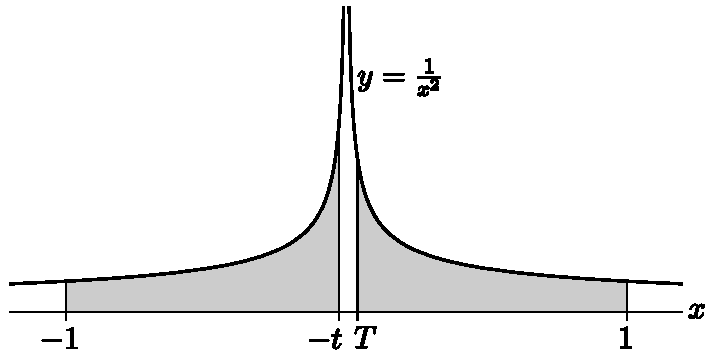
\includegraphics{boobyTrap}
\end{center}
\end{efig}
The full domain of integration is only recovered in the limit
$t,T\rightarrow 0$.

\item For this example, the correct computation is
\begin{align*}
%$$\eqalign{
\int_{-1}^1\frac{1}{x^2}\dee{x}
&=\lim_{t\rightarrow 0^+}\int_{-1}^{-t}\frac{1}{x^2}\dee{x}
\ +\ \lim_{T\rightarrow 0^+}\int_{T}^{1}\frac{1}{x^2}\dee{x} \\[0.05in]
&=\lim_{t\rightarrow 0^+}\bigg[-\frac{1}{x}\bigg]_{-1}^{-t}
+\lim_{T\rightarrow 0^+}\bigg[-\frac{1}{x}\bigg]_{T}^1
               \displaybreak[0]\\[0.05in]
&=\lim_{t\rightarrow 0^+}
       \Big[\Big(-\frac{1}{-t}\Big)-\Big(-\frac{1}{-1}\Big)\Big]
+\lim_{T\rightarrow 0^+}
         \Big[\Big(-\frac{1}{1}\Big)-\Big(-\frac{1}{T}\Big)\Big]
               \displaybreak[0]\\[0.05in]
&=\lim_{t\rightarrow 0^+}\frac{1}{t}
  +\lim_{T\rightarrow 0^+}\frac{1}{T}-2 \\[0.05in]
&=+\infty
\end{align*}
\item We can interpret this to mean that the signed area under the curve $x^{-2}$ between
$x=-1$ and $x=1$ is infinite.
\end{itemize}
\end{comment}

\end{eg}

The above examples have illustrated how we can use the fundamental
theorem of calculus to convert knowledge of derivatives into
knowledge of integrals.
We are now in a position to easily build a table of integrals. Here is
a short table of the most important derivatives that we know.

\begin{center}
\renewcommand{\arraystretch}{1.3}
   \begin{tabular}{!{\vrule width 1pt}c!{\vrule width
1pt}c|c|c|c|c|c|c|c|c!{\vrule width 1pt}}
        \noalign{\hrule height 1pt}
        $F(x)$  & $1$ & $x^n$      & $\sin x$ & $\cos x$ & $\tan x$ &
$e^x$ & $\log_e|x|$       & $\arcsin x$             & $\arctan x$ \\    \hline
        $f(x)=F'(x)$ & $0$ & $nx^{n-1}$ & $\cos x$ & $-\sin x$ & $\sec^2 x$ &
$e^x$ & $\frac{1}{x}$ &
$\frac{1}{\sqrt{1-x^2}}$
      & $\frac{1}{1+x^2}$ \\
      \noalign{\hrule height 1pt}
     \end{tabular}
\renewcommand{\arraystretch}{1.0}
\end{center}
Of course we know other derivatives, such as those of $\sec x$ and $\cot x$, however the
ones listed above are arguably the most important ones. From this table (with a very
little massaging) we can write down a short table of indefinite integrals.
\begin{theorem}[Important indefinite integrals]\label{thm imp indef int}

\begin{center}
% \renewcommand{\arraystretch}{1.4}
%      \begin{tabular}{!{\vrule width 1pt}c|c!{\vrule width 1pt}}
%         \noalign{\hrule height 1pt}
%     $f(x)$ & $ F(x)=\int f(x)\dee{x}$ \\
%         \noalign{\hrule height 1pt}
% %  powers
%     $1$ & $x+C$ \\  \hline
%     $x^n$ & \raisebox{2pt}{$\frac{1}{n+1}x^{n+1}+C\hbox{ if }n \ne-1$} \\  \hline
%     \raisebox{2pt}{$\frac{1}{x}$} & $\ln|x|+C$ \\  \hline
% % trig
%     $\sin x$ & $-\cos x+C$ \\  \hline
%     $\cos x$ & $\sin x+C$ \\  \hline
%     $\sec^2 x$ & $\tan x+C$ \\  \hline
% % exp
%     $e^x$ & $e^x+C$ \\ \hline
% % inverse trig
%     \raisebox{2pt}{$\frac{1}{\sqrt{1-x^2}}$} & $\arcsin x+C$ \\  \hline
%     \raisebox{2pt}{$\frac{1}{1+x^2}$} & $\arctan x+C$ \\
%       \noalign{\hrule height 1pt}
%      \end{tabular}
% \renewcommand{\arraystretch}{1.0}

\renewcommand{\arraystretch}{2.5}
     \begin{tabular}{|c|c|}
        \hline
    $f(x)$ & $ F(x)=\int f(x)\dee{x}$ \\
        \hline\hline
%  powers
    $1$ & $x+C$ \\  \hline
    $x^n$ & $\frac{1}{n+1}x^{n+1}+C\text{ provided that }n \ne-1$ \\  \hline
%log
    $\dfrac{1}{x}$ & $\log_e|x|+C$ \\  \hline\hline
% exp
    $e^x$ & $e^x+C$ \\ \hline\hline
% trig
    $\sin x$ & $-\cos x+C$ \\  \hline
    $\cos x$ & $\sin x+C$ \\  \hline
    $\sec^2 x$ & $\tan x+C$ \\  \hline\hline
% inverse trig
   $\dfrac{1}{\sqrt{1-x^2}}$ & $\arcsin x+C$ \\  \hline
  $\dfrac{1}{1+x^2}$ & $\arctan x+C$ \\
   \hline
     \end{tabular}
\renewcommand{\arraystretch}{1.0}

\end{center}
\end{theorem}

\begin{eg}
 Find the following integrals
\begin{enumerate}[(i)]
 \item $\int_2^7 e^x \dee{x}$
 \item $\int_{-2}^2 \frac{1}{1+x^2} \dee{x}$
 \item $\int_0^3 (2x^3+7x-2)\dee{x}$
\end{enumerate}
\soln We can proceed with each of these as before --- find the antiderivative and then
apply the fundamental theorem. The third integral is a little more complicated, but we
can split it up into monomials using Theorem~\ref{thm:Intarith} and do each separately.
\begin{enumerate}[(i)]
 \item An antiderivative of $e^x$ is just $e^x$, so
\begin{align*}
  \int_2^7 e^x \dee{x} &= e^x\bigg|_2^7 \\
  &= e^7-e^2 = e^2(e^5-1).
\end{align*}
\item An antiderivative of $\frac{1}{1+x^2}$ is $\arctan(x)$, so
\begin{align*}
    \int_{-2}^2 \frac{1}{1+x^2} \dee{x}
  &= \arctan(x) \bigg|_{-2}^2 \\
  &= \arctan(2) - \arctan(-2)
\intertext{We can simplify this a little further by noting that $\arctan(x)$ is an
odd function, so $\arctan(-2)= -\arctan(2)$
and thus our integral is}\\
  &= 2\arctan(2)
\end{align*}
\item We can proceed by splitting the integral using Theorem~\ref{thm:Intarith}(d)
\begin{align*}
  \int_0^3 (2x^3+7x-2)\dee{x}
&= \int_0^3 2x^3\dee{x} + \int_0^3 7x\dee{x} - \int_0^3 2\dee{x}\\
&= 2\int_0^3 x^3\dee{x} + 7\int_0^3 x\dee{x} - 2\int_0^3 \dee{x}
\intertext{and because we know that $x^4/4, x^2/2, x$ are antiderivatives of $x^3, x, 1$
respectively, this becomes}
&= \left[\frac{x^4}{2}\right]_0^3 + \left[\frac{7x^2}{2}\right]_0^3 - \left[2x\right]_0^3
\\
&= \frac{81}{2} + \frac{7\cdot 9}{2} -6\\
&= \frac{81 + 63 - 12}{2} = \frac{132}{2} = 66.
\end{align*}
We can also just find the antiderivative of the whole polynomial by finding the
antiderivatives of each term of the polynomial and then recombining them. This is
equivalent to what we have done above, but perhaps a little neater:
\begin{align*}
 \int_0^3 (2x^3+7x-2)\dee{x}
&= \left[ \frac{x^4}{2} + \frac{7x^2}{2} - 2x \right]_0^3 \\
&= \frac{81}{2} + \frac{7\cdot 9}{2} -6 = 66.
\end{align*}
\end{enumerate}

\end{eg}



\section{Substitution}\label{sec subs}
In the previous section we explored the fundamental theorem of calculus and the link it
provides between definite integrals and antiderivatives. Indeed, integrals with simple
integrands are usually evaluated via this link. In this section we start to explore
methods for integrating more complicated integrals. We have already seen ---
via Theorem~\ref{thm:Intarith} --- that integrals interact very nicely with
addition, subtraction and multiplication by constants:
\begin{align*}
  \int_a^b \left( Af(x) + B g(x) \right) \dee{x}
  &= A\int_a^b f(x)\dee{x} + B\int_a^b g(x)\dee{x}
\end{align*}
for $A,B$ constants. By combining this with the list of indefinite integrals in
Theorem~\ref{thm imp indef int}, we can compute integrals of linear combinations of
simple functions. For example
\begin{align*}
  \int_1^4\left(e^x - 2\sin x + 3x^2 \right)\dee{x}
  &= \int_1^4e^x\dee{x} -2\int_1^4 \sin x \dee{x} +3 \int_1^4x^2 \dee{x}\\
  &= \left(e^x  + (-2)\cdot(-\cos x) + 3\frac{x^3}{3} \right)\bigg|_1^4
&\text{and so on}
\end{align*}
Of course there are a great many functions that can be approached in this way, however
there are some very simple examples that cannot.
\begin{align*}
  \int \sin(\pi x) \dee{x}
  && \int x e^x \dee{x}
  && \int \frac{x}{x^2-5x+6}\dee{x}
\end{align*}
In each case the integrands are not linear combinations of simpler functions; in order to
compute them we need to understand how integrals (and antiderivatives) interact with
compositions, products and quotients. We reached a very similar point in our differential
calculus course where we understood the linearity of the derivative,
\begin{align*}
  \diff{}{x}\left(Af(x)+ Bg(x)\right) &= A\diff{f}{x} + B\diff{g}{x},
\end{align*}
but had not yet seen the chain, product and quotient rules\footnote{If your memory of
these rules is a little hazy then you really should go back and revise them before
proceeding. You will definitely need a good grasp of the chain rule for what follows in
this section.}. While we will develop tools to find the second and third integrals in
later sections, we should really start with how to integrate compositions of functions.

It is important to state up front, that in general one cannot write down the integral of
the composition of two functions --- even if those functions are simple. This is not
because the integral does not exist. Rather it is because the integral cannot be written
down as a finite combination of the standard functions we know. A very good example of
this, which we encountered in Example~\ref{eg:INTftocA}, is the composition of $e^x$ and
$-x^2$. Even though we know
\begin{align*}
  \int e^x \dee{x} &= e^x+C & \text{and}&&
  \int -x^2 \dee{x} &= -\frac13 x^3 +C
\end{align*}
there is no simple function that is equal to the indefinite integral
\begin{align*}
\int e^{-x^2}\dee{x}.
\end{align*}
even though the indefinite integral exists. In this way integration is very different
from differentiation.

With that caveat out of the way, we can introduce the substitution rule. The substitution
rule is obtained by antidifferentiating the chain rule. In some sense it is the chain
rule
in reverse. For completeness, let us restate the chain rule:
\begin{theorem}[The chain rule]
  Let $F(u)$ and $u(x)$ be differentiable functions and form their composition $F(u(x))$.
Then
  \begin{align*}
  \diff{}{x} F\big( u( x) \big) &= F'\big(u(x)\big) \cdot u'(x)
\end{align*}
Equivalently, if $y(x)=F(u(x))$, then
\begin{align*}
  \diff{y}{x} &= \diff{F}{u} \cdot \diff{u}{x}.
\end{align*}
\end{theorem}


Consider a function $f(u)$, which has antiderivative $F(u)$. Then we know
that
\begin{align*}
  \int f(u) \dee{u} &= \int F'(u) \dee{u} = F(u) +C
\end{align*}
Now take the above equation and substitute into it $u=u(x)$ --- i.e. replace the
variable $u$ with any (differentiable) function of $x$ to get
\begin{align*}
\int f(u) \dee{u}\bigg|_{u=u(x)} &= F(u(x)) +C
\end{align*}
But now the right-hand side is a function of $x$, so we can differentiate it with respect
to $x$ to get
\begin{align*}
  \diff{}{x} F(u(x)) &= F'(u(x)) \cdot u'(x)
\end{align*}
This tells us that $F(u(x))$ is an antiderivative of the function $F'(u(x))\cdot u'(x)
= f(u(x))u'(x)$. Thus we know
\begin{align*}
    \int f\big(u(x)\big) \cdot u'(x)\,\dee{x}
      &= F\big(u(x)\big) +C
      = \int f(u)\,\dee{u}\bigg|_{u=u(x)}
\end{align*}
This is the substitution rule for indefinite integrals.
%%%
\begin{theorem}[The substitution rule --- indefinite integral version]\label{thm subs
indef}
 For any differentiable function $u(x)$:
\begin{align*}
  \int f(u(x)) u'(x) \dee{x} &= \int f(u)\dee{u}\bigg|_{u=u(x)}
\end{align*}
\end{theorem}
%%%
In order to apply the substitution rule successfully we will have to write the integrand
in the form $f(u(x))\cdot u'(x)$. To do this we need to make a good choice of the
function $u(x)$; after that it is not hard to then find $f(u)$ and $u'(x)$.
Unfortunately there is no one strategy for choosing $u(x)$. This can make applying the
substitution rule more art than science\footnote{Thankfully this does become easier with
experience and we recommend that the reader read some examples and then practice a LOT.}.
Here we suggest two possible strategies for picking $u(x)$:
\begin{enumerate}[(1)]
\item Factor the integrand and choose one of the factors to be $u'(x)$. For this to work,
you must be able to easily find the antiderivative of the chosen factor. The
antiderivative will be $u(x)$.
\item Look for a factor in the integrand that is a function with an argument that is more
complicated than just ``$x$''. That factor will play the role of $f\big(u(x)\big)$ Choose
$u(x)$ to be the complicated argument.
\end{enumerate}
Here are two examples which illustrate each of those strategies in turn.
\begin{eg}
Consider the integral
\begin{align*}
  \int 9\sin^8(x) \cos(x) \dee{x}
\end{align*}
We want to massage this into the form of the integrand in the substitution rule --- namely
$f(u(x))\cdot u'(x)$. Our integrand can be written as the product of the two factors
\begin{align*}
\underbrace{9 \sin^8(x)}_\text{first factor} \cdot
\underbrace{\cos(x)}_\text{second factor}
\end{align*}
and we start by determining (or guessing) which factor plays the role of
$u'(x)$. We can choose $u'(x)=9\sin^8(x)$ or $u'(x)=\cos(x)$.
\begin{itemize}
 \item If we choose $u'(x)=9\sin^8(x)$, then antidifferentiating this to find $u(x)$ is
really not very easy. So it is perhaps better to investigate the other choice before
proceeding further with this one.
\item If we choose $u'(x)=\cos(x)$, then we know (Theorem~\ref{thm imp indef int}) that
$u(x)=\sin(x)$. This also works nicely because it makes the other factor
simplify quite a bit $9\sin^8(x) = 9u^8$. This looks like the right way to go.
\end{itemize}
So we go with the second choice. Set $u'(x)=\cos(x), u(x)=\sin(x)$, then
\begin{align*}
  \int 9\sin^8(x) \cos(x) \dee{x}
  &= \int 9u(x)^8 \cdot u'(x) \dee{x} \\
  &= \int 9u^8 \dee{u} \bigg|_{u=\sin(x)} & \text{by the substitution rule}
\intertext{We are now left with the problem of antidifferentiating a monomial; this we
can
do with Theorem~\ref{thm imp indef int}.}
  &= \left( u^9 +C \right)\bigg|_{u=\sin(x)}\\
  &= \sin^9(x) +C
\end{align*}
Note that $9\sin^8(x) \cos(x)$ is a function of $x$. So our answer, which is the
indefinite integral of  $9\sin^8(x) \cos(x)$, must also be a function of $x$.
This is why we have substituted $u=\sin(x)$ in the last step of our solution --- it
makes our solution a function of $x$.
\end{eg}
\begin{eg}
 Evaluate the integral
\begin{align*}
\int 3x^2 \cos(x^3) \dee{x}
\end{align*}
\soln Again we are going to use the substitution rule and helpfully our integrand is a
product of two factors
\begin{align*}
\underbrace{3x^2}_\text{first factor} \cdot
\underbrace{\cos(x^3)}_\text{second factor}
\end{align*}
The second factor, $\cos\big(x^3\big)$ is a function, namely $\cos$, with a complicated
argument, namely $x^3$. So we try $u(x)= x^3$. Then $u'(x) = 3x^2$, which is the other
factor in the integrand. So the integral becomes
\begin{align*}
  \int 3x^2 \cos(x^3) \dee{x}
&= \int u'(x) \cos\big(u(x)\big) \dee{x} &\text{just swap order of factors}\\
&= \int \cos\big(u(x)\big) u'(x) \dee{x} & \text{by the substitution rule}\\
&= \int \cos(u) \dee{u}\bigg|_{u=x^3} \\
&= \left( \sin(u) + C\right)\bigg|_{u=x^3}  & \text{using Theorem~\ref{thm imp indef
int})}\\
&= \sin(x^3)+C
\end{align*}
\end{eg}
One more --- we'll use this to show how to use the substitution rule with definite
integrals.
\begin{eg}[$\int_0^1 e^x\sin(e^x)\dee{x}$]\label{eg:substitution1}
Compute
\begin{align*}
  \int_0^1 e^x\sin\big(e^x\big)\dee{x}.
\end{align*}
\soln Again we use the substitution rule.
\begin{itemize}
 \item The integrand is again the product of two factors and we can choose $u'(x)=e^x$ or
$u'(x)=\sin(e^x)$.
\item If we choose $u'(x)=e^x$ then $u(x)=e^x$ and the other factor becomes $\sin(u)$ ---
this looks promising. Notice that if we applied the other strategy of looking for a
complicated argument then we would arrive at the same choice.

\item So we try $u'(x)=e^x$ and $u(x)=e^x$. This gives (if we ignore the limits of
integration for a moment)
\begin{align*}
  \int e^x \sin\big(e^x\big)\dee{x}
&= \int \sin\big(u(x)\big) u'(x) \dee{x} &\text{apply the substitution rule}\\
&= \int \sin(u)\dee{u} \bigg|_{u=e^x}\\
&= \left(-\cos(u)+C \right)\bigg|_{u=e^x}\\
&= -\cos\big(e^x\big) +C
\end{align*}
\item But what happened to the limits of integration? We can incorporate them now. We
have just shown that the indefinite integral is $-\cos(e^x)$, so by the fundamental
theorem of calculus
\begin{align*}
  \int_0^1 e^x\sin\big(e^x\big)\dee{x}
  &= \big[-\cos\big(e^x\big)\big]_0^1\\
  &= -\cos(e^1)-(-\cos(e^0)) \\
  &= -\cos(e)+\cos(1)
\end{align*}
% \item We can also do the following:
% \begin{align*}
% \int_0^1 e^x \sin\big(e^x\big)\dee{x}
% &= \int_0^1 \sin(u) u'(x) \dee{x} &\text{apply the substitution rule}\\
% &= \int_{u(0)}^{u(1)} \sin(u)\dee{u} &\text{since this is now in terms of $u$}\\
% &= \left[-\cos(u) \right]_{u(0)}^{u(1)} & \text{where }u(0)=1, u(1)=e \\
% &= -\cos(e) + \cos(1)
% \end{align*}
\end{itemize}
\end{eg}
Theorem~\ref{thm subs indef}, the substitution rule for indefinite integrals, tells us
that if $F(u)$ is any antiderivative for $f(u)$, then $F\big(u(x)\big)$ is an
antiderivative for $f\big(u(x)\big) u'(x)$. So the fundamental theorem of calculus gives
us
\begin{align*}
  \int_a^b f\big(u(x)\big) u'(x)\,\dee{x}
  &= F\big(u(x)\big)\bigg|_{x=a}^{x=b} \\
  &= F\big(u(b)\big) - F\big(u(a)\big) \\
  &= \int_{u(a)}^{u(b)} f(u)\,\dee{u}
  & \text{since $F(u)$ is an antiderivative for $f(u)$}
\end{align*}
and we have just found
%%%
\begin{theorem}[The substitution rule --- definite integral version]\label{thm subs
def}
 For any differentiable function $u(x)$:
\begin{align*}
  \int_a^b f(u(x)) u'(x) \dee{x} &= \int_{u(a)}^{u(b)} f(u)\dee{u}
\end{align*}
\end{theorem}
%%%
Notice that to get from the integral on the left hand side to the integral on the right
hand side you
\begin{itemize}
\item substitute\footnote{A good way to remember this last step is that we
replace $\diff{u}{x} \dee{x}$ by just $\dee{u}$ --- which looks
like we cancelled out the $\dee{x}$ terms:
$\frac{\dee{u}}{\cancel{\dee{x}}}\cancel{\dee{x}} = \dee{u}$. While using ``cancel the
$\dee{x}$'' is a good mnemonic (memory aid), you should not think of the derivative
$\diff{u}{x}$ as a fraction --- you are not dividing $\dee{u}$ by $\dee{x}$. }
$u(x)\rightarrow u$ and
$u'(x)\dee{x}\rightarrow \dee{u}$,
  \item set the lower limit for the $u$ integral to the value of
    $u$ (namely $u(a)$) that corresponds to the lower limit of the $x$
    integral (namely $x=a$), and
  \item set the upper limit for the $u$ integral to the value of
    $u$ (namely $u(b)$) that corresponds to the upper limit of the $x$
    integral (namely $x=b$).
\end{itemize}
Also note that we now have two ways to evaluate definite integrals of the form
$\int_a^b f\big(u(x)\big)u'(x)\,\dee{x}$.
\begin{itemize}
\item We can find the indefinite integral $\int f\big(u(x)\big) u'(x)\,\dee{x}$, using
Theorem~\ref{thm subs indef}, and then evaluate the result between $x=a$ and $x=b$. This
is what was done in Example~\ref{eg:substitution1}.
\item Or we can apply Theorem~\ref{thm subs indef}. This entails finding the
indefinite integral $\int f(u)\,\dee{u}$ and evaluating the result between $u=u(a)$ and
$u=u(b)$. This is what we will do in the following example.
\end{itemize}

\begin{eg}[$ \int_0^1 x^2\sin(x^3+1)\dee{x}$]\label{eg:substitution2}
Compute
\begin{align*}
  \int_0^1 x^2\sin\big(x^3+1\big)\dee{x}
\end{align*}
\soln
\begin{itemize}
 \item In this example the integrand is already neatly factored into two pieces. While we
could deploy either of our two strategies, it is perhaps easier in this case to
choose $u(x)$ by looking for a complicated argument.
\item The second factor of the integrand is $\sin\big(x^3+1\big)$, which is the function
$\sin$ evaluated at $x^3+1$. So set $u(x)=x^3+1$, giving $u'(x)=3x^2$ and $f(u)=\sin(u)$
\item The first factor of the integrand is $x^2$ which is not quite $u'(x)$, however we
can easily massage the integrand into the required form by multiplying and dividing by
$3$:
\begin{align*}
  x^2\sin\big(x^3+1\big) &= \frac{1}{3} \cdot 3x^2\cdot \sin\big(x^3+1\big).
\end{align*}
\item We want this in the form of the substitution rule, so we do a little massaging:
\begin{align*}
  \int_0^1 x^2\sin\big(x^3+1\big)\dee{x}
  &= \int_0^1 \frac{1}{3}\cdot 3x^2 \cdot \sin\big(x^3+1\big)\dee{x}\\
  &= \frac{1}{3}\int_0^1 \sin\big(x^3+1\big)\cdot 3x^2 \dee{x}
&\text{by Theorem~\ref{thm:Intarith}(c)}
\end{align*}
\item Now we are ready for the substitution rule:
\begin{align*}
\frac{1}{3}\int_0^1 \sin\big(x^3+1\big)\cdot 3x^2 \dee{x}
&=\frac{1}{3}\int_0^1 \underbrace{\sin\big(x^3+1\big)}_{=f(u(x))}\cdot
\underbrace{3x^2}_{=u'(x)} \dee{x}\\
&= \frac{1}{3}\int_0^1 f(u(x)) u'(x) \dee{x}
&\text{with $u(x)=x^3+1$ and $f(u)=\sin(u)$}\\
&= \frac{1}{3} \int_{u(0)}^{u(1)} f(u) \dee{u} & \text{by the substitution rule} \\
&= \frac{1}{3} \int_{1}^{2} \sin(u) \dee{u}  & \text{since $u(0)=1$ and
$u(1)=2$}\\
&= \frac{1}{3} \big[-\cos(u)\big]_1^2 \\
&= \frac{1}{3}\big( -\cos(2) -(-\cos(1)) \big)\\
&= \frac{\cos(1)-\cos(2)}{3}.
\end{align*}
\end{itemize}
\end{eg}

There is another, and perhaps easier, way to view the manipulations in the previous
example. Once you have chosen $u(x)$ you
\begin{itemize}
 \item make the substitution $u(x) \rightarrow u$,
 \item replace $\dee{x} \rightarrow \dfrac{1}{u'(x)} \dee{u}$.
\end{itemize}
In so doing, we take the integral
\begin{align*}
  \int_a^b f(u(x)) \cdot u'(x) \dee{x}
&= \int_{u(a)}^{u(b)} f(u) \cdot u'(x) \cdot \frac{1}{u'(x)} \dee{u} \\
&= \int_{u(a)}^{u(b)} f(u) \dee{u} & \text{exactly the substitution rule}
\end{align*}
but we do not have to manipulate the integrand so as to make $u'(x)$ explicit.  Let us
redo the previous example by this approach.

% Once one has chosen $u(x)$, one can make the substitution without ever
% explicitly deciding what $f(u)$ is. One just has to note that the
% integrand on the right hand side of the substitution rule
% \begin{align*}
% \int_a^b f\big(u(x)\big)\,u'(x)\dee{x}=\int_{u(a)}^{u(b)} f(u)\,\dee{u}
% \end{align*}
% is constructed from the integrand on the left hand side by
% \begin{itemize}
% \item substituting $u$ for $u(x)$ and
% \item substituting $\dee{u}$ for $u'(x)\dee{x}$
% \end{itemize}
% The substitution $\dee{u}=u'(x)\dee{x}$ is easily remembered by \emph{pretending} that
% $\tfrac{\dee{u}}{\dee{x}}$ is an ordinary fraction. Then cross--multiplying
% $\tfrac{\dee{u}}{\dee{x}}=u'(x)$ gives $\dee{u}=u'(x)\dee{x}$.
%
% \medskip
\begin{eg}[\emph{Example \ref{eg:substitution2} revisited}]
                                               \label{eg:substitution3}
Compute the integral
\begin{align*}
\int_0^1 x^2\sin\big(x^3+1\big)\dee{x}
\end{align*}
\soln
\begin{itemize}
 \item We have already observed that one factor of the integrand is
$\sin\big(x^3+1\big)$, which is $\sin$ evaluated at $x^3+1$. Thus we try setting
$u(x)=x^3+1$.
\item This makes $u'(x)=3x^2$, and we replace $u(x)=x^3+1\rightarrow u$ and
$\dee{x}\rightarrow\frac{1}{u'(x)}\dee{u} = \frac{1}{3x^2}\dee{u}$:
\begin{align*}
  \int_0^1 x^2\sin\big(x^3+1\big)\dee{x}
&= \int_{u(0)}^{u(1)} x^2\underbrace{\sin\big(x^3+1\big)}_{=\sin(u)}
\frac{1}{3x^2}\dee{u} \\
&= \int_{1}^{2} \sin(u) \frac{x^2}{3x^2}\dee{u}\\
&= \int_{1}^{2} \frac{1}{3}\sin(u) \dee{u} \\
&= \frac{1}{3}\int_{1}^{2} \sin(u) \dee{u}
\end{align*}
which is precisely the integral we found in Example~\ref{eg:substitution2}.
\end{itemize}

\end{eg}

\begin{eg}
Compute the indefinite integrals
\begin{align*}
  \int \sqrt{2x+1}\dee{x} && \text{and} && \int e^{3x-2}\dee{x}
\end{align*}
\soln
\begin{itemize}
 \item Starting with the first integral, we see that it is not too hard to spot
the complicated argument. If we set $u(x)=2x+1$ then the integrand is just $\sqrt{u}$.
\item Hence we substitute $2x+1 \rightarrow u$ and $\dee{x} \rightarrow
\frac{1}{u'(x)}\dee{u}=\frac{1}{2}\dee{u}$:
\begin{align*}
  \int \sqrt{2x+1}\dee{x}
&= \int \sqrt{u} \frac{1}{2} \dee{u} \\
&= \int u^{1/2} \frac{1}{2} \dee{u} \\
&= \left( \frac{2}{3}u^{3/2}\cdot\frac{1}{2}  +C\right)\bigg|_{u=2x+1}\\
&= \frac{1}{3} (2x+1)^{3/2} + C
\end{align*}
\item We can evaluate the second integral in much the same way. Set $u(x)=3x-2$ and
replace $\dee{x}$ by $\frac{1}{u'(x)}\dee{u} = \frac{1}{3}\dee{u}$:
\begin{align*}
  \int e^{3x-2}\dee{x}
&= \int e^u \frac{1}{3}\dee{u} \\
&= \left( \frac{1}{3} e^u + C\right)\bigg|_{u=3x-2}\\
&= \frac{1}{3} e^{3x-2} +C
\end{align*}
\end{itemize}
\end{eg}
This last example illustrates that substitution can be used to easily deal 
with arguments of the form $ax+b$ (with $a,b$ constants and $a\ne 0$), i.e. 
that are linear functions of $x$, and suggests the following theorem.
\begin{theorem}\label{thm subs linear}
Let $F(u)$ be an antiderivative of $f(u)$ and let $a,b$ be constants 
with $a\ne 0$. Then
\begin{align*}
  \int f(ax+b)\dee{x} &= \frac{1}{a} F(ax+b) +C
\end{align*}
\end{theorem}
\begin{proof}
 We can show this using the substitution rule. Let $u(x)=ax+b$ so $u'(x)=a$, then
\begin{align*}
  \int f(ax+b) \dee{x}
&= \int f(u) \cdot \frac{1}{u'(x)}\dee{u}\\
&= \int \frac{1}{a} f(u) \dee{u} \\
&= \frac{1}{a} \int f(u) \dee{u} & \text{since $a$ is a constant}\\
&= \frac{1}{a} F(u)\bigg|_{u=ax+b} +C & \text{since $F(u)$ is an antiderivative of
$f(u)$}\\
&= \frac{1}{a} F(ax+b) +C.
\end{align*}
\end{proof}
Now we can do the following example using the substitution rule or the above theorem:
\begin{eg}[$\int_0^{\nicefrac{\pi}{2}}\cos(3x)\dee{x}$]\label{eg:substitution4}
Compute $\int_0^{\nicefrac{\pi}{2}}\cos(3x)\dee{x}$.

\begin{itemize}
 \item In this example we should set $u=3x$, and substitute $\dee{x} \rightarrow
\frac{1}{u'(x)}\dee{u} = \frac{1}{3}\dee{u}.$ When we do this we also have to convert
the limits of the integral: $u(0)=0$ and $u(\pi/2)=3\pi/2$. This gives
\begin{align*}
  \int_0^{\nicefrac{\pi}{2}}\cos(3x)\dee{x}
&= \int_0^{\nicefrac{3\pi}{2}} \cos(u) \frac{1}{3}\dee{u}\\
&= \left[\frac{1}{3} \sin(u) \right]_0^{\nicefrac{3\pi}{2}}\\
&= \frac{\sin(3\pi/2)-\sin(0)}{3}\\
&= \frac{-1-0}{3} = - \frac{1}{3}.
\end{align*}
\item We can also do this example more directly using the above theorem. Since $\sin(x)$
is an antiderivative of $\cos(x)$, Theorem~\ref{thm subs linear} tells us that
$\frac{\sin(3x)}{3}$ is an antiderivative of $\cos(3x)$. Hence
\begin{align*}
  \int_0^{\nicefrac{\pi}{2}}\cos(3x)\dee{x}
&= \left[ \frac{\sin(3x)}{3} \right]_0^{\nicefrac{\pi}{2}}\\
&= \frac{\sin(3\pi/2)-\sin(0)}{3}\\
&= -\frac{1}{3}.
\end{align*}
\end{itemize}

\end{eg}

The rest of this section is just more examples of the substitution rule. We recommend
that you after reading these that you practice many examples by yourself under exam
conditions.

\begin{eg}[$ \int_0^1 x^2\sin(1-x^3)\dee{x}$]   \label{eg:substitution3neg}
This integral looks a lot like that of Example \ref{eg:substitution2}. It makes
sense to try $u(x)=1-x^3$ since it is the argument of $\sin(1-x^3)$. We
\begin{itemize}
\item substitute $u=1-x^3$ and
\item replace $\dee{x}$ with $\frac{1}{u'(x)}\dee{u} = \frac{1}{-3x^2}\dee{u}$,
\item  when $x=0$, we have $u=1-0^3=1$ and
\item  when $x=1$, we have $u=1-1^3=0$.
\end{itemize}
So
\begin{align*}
  \int_0^1 x^2 \sin\big(1-x^3\big)\cdot \dee{x}
  &=\int_1^0 x^2 \sin(u) \cdot \frac{1}{-3x^2}\dee{u} \\
  &= \int_1^0 -\frac{1}{3}\sin(u)\dee{u}.
\intertext{Note that the lower limit of the $u$--integral, namely $1$,
is larger than the upper limit, which is $0$. There is absolutely
nothing wrong with that. We can simply evaluate the $u$--integral
in the normal way. Since $-\cos(u)$ is an antiderivative
of $\sin(u)$:}
&=  \left[\frac{\cos(u)}{3} \right]_1^0 \\
&= \frac{\cos(0)-\cos(1)}{3}\\
&= \frac{1-\cos(1)}{3}.
\end{align*}
\end{eg}

\begin{eg}[$\int_0^1\frac{1}{(2x+1)^3}\dee{x}$]\label{eg:substitution5}
Compute $\int_0^1\frac{1}{(2x+1)^3}\dee{x}$.

We could do this one using Theorem~\ref{thm subs linear}, but its not too hard to do
without. We can think of the integrand as the function ``one over a cube'' with
the argument $2x+1$. So it makes sense to substitute $u=2x+1$. That is
\begin{itemize}
\item set $u=2x+1$ and
\item replace $\dee{x} \rightarrow \frac{1}{u'(x)}\dee{u} =
\frac{1}{2}\dee{u}$.
\item When $x=0$, we have $u=2\times 0+1=1$ and
\item when $x=1$, we have $u=2\times 1+1=3$.
\end{itemize}
So
\begin{align*}
  \int_0^1\frac{1}{(2x+1)^3}\dee{x}
  &=\int_1^{3} \frac{1}{u^3} \cdot \frac{1}{2}\dee{u} \\
  &=\frac{1}{2}\int_1^{3}u^{-3}\dee{u}\\
  &=\frac{1}{2}\left[\frac{u^{-2}}{-2}\right]_1^{3}\\
  &=\frac{1}{2}\left( \frac{1}{-2}\cdot \frac{1}{9} - \frac{1}{-2}\cdot\frac{1}{1}
\right)\\
  &=\frac{1}{2}\left( \frac{1}{2} - \frac{1}{18}\right) = \frac{1}{2}\cdot \frac{8}{18}\\
  &=\frac{2}{9}
\end{align*}
\end{eg}

\begin{eg}[$\int_0^1\frac{x}{1+x^2}\dee{x}$]\label{eg:substitution6}
Evaluate $\int_0^1\frac{x}{1+x^2}\dee{x}$.

\soln
\begin{itemize}
 \item The integrand can be rewritten as $x \cdot \frac{1}{1+x^2}$. This second factor
suggests that we should try setting $u=1+x^2$ --- and so we interpret the
second factor as the function ``one over'' evaluated at argument $1+x^2$.
\item With this choice we
\begin{itemize}
\item set $u=1+x^2$,
\item substitute $\dee{x} \rightarrow \frac{1}{2x}\dee{u}$, and
\item translate the limits of integration: when $x=0$, we have $u=1+0^2=1$ and when
$x=1$, we have $u=1+1^2=2$.
\end{itemize}
\item The integral then becomes
\begin{align*}
\int_0^1\frac{x}{1+x^2}\dee{x}
&= \int_1^2 \frac{x}{u} \frac{1}{2x}\dee{u} \\
&= \int_1^2 \frac{1}{2u} \dee{u} \\
&= \frac{1}{2} \big[ \log|u| \big]_1^2 \\
&= \frac{\log 2 - \log 1}{2} = \frac{\log 2}{2}.
\end{align*}
\end{itemize}
Remember that we are using the notation ``$\log$'' for the natural
logarithm, i.e. the logarithm with base $e$. You might also see it written as ``$\ln
x$'', or with the base made explicit as ``$\log_e x$''.
\end{eg}

\begin{eg}[$\int x^3\cos\big(x^4+2\big)\dee{x}$]\label{eg:substitution7}
Compute the integral $\int x^3\cos\big(x^4+2\big)\dee{x}$.


\soln
\begin{itemize}
 \item The integrand is the product of $\cos$ evaluated at the argument $x^4+2$ times
$x^3$, which aside from a factor of $4$, is the derivative of the argument $x^4+2$.
\item Hence we set $u=x^4+2$ and then substitute $\dee{x} \rightarrow
\frac{1}{u'(x)}\dee{u} = \frac{1}{4x^3}\dee{u}$.

\item Before proceeding further, we should note that  this is an indefinite integral so
we
don't have to worry about the limits of integration. However we do need to make sure our
answer is a function of $x$ --- we cannot leave it as a function of $u$.

\item With this choice of $u$, the integral then becomes
\begin{align*}
  \int x^3\cos\big(x^4+2\big)\dee{x}
&= \int x^3 \cos(u) \frac{1}{4x^3}\dee{u} \bigg|_{u=x^4+2}\\
&=  \int\frac{1}{4} \cos(u) \dee{u} \bigg|_{u=x^4+2}\\
&= \left(\frac{1}{4}\sin(u)+C\right)\bigg|_{u=x^4+2} \\
&= \frac{1}{4}\sin(x^4+2) +C.
\end{align*}
\end{itemize}


\end{eg}
The next two examples are more involved and require more careful thinking.

\begin{eg}[$\int \sqrt{1+x^2}\,x^3\dee{x}$]\label{eg:substitution8}
Compute $\int \sqrt{1+x^2}\,x^3\dee{x}$.

\begin{itemize}
 \item An obvious choice of $u$ is the argument inside the square root. So substitute
$u=1+x^2$ and $\dee{x} \rightarrow \frac{1}{2x}\dee{u}$.
\item When we do this we obtain
\begin{align*}
  \int \sqrt{1+x^2}\cdot x^3\dee{x}
  &= \int \sqrt{u}\cdot x^3 \cdot \frac{1}{2x}\dee{u}\\
  &= \int \frac{1}{2} \sqrt{u}\cdot x^2 \dee{u}
\end{align*}
Unlike all our previous examples, we have not cancelled out all of the $x$'s from the
integrand. However before we do the integral with respect to $u$, the integrand must be
expressed solely in terms of $u$ --- no $x$'s are allowed. (Look that integrand on the
right hand side of Theorem~\ref{thm subs indef}.)

\item But all is not lost. We can rewrite the factor $x^2$ in terms of the variable $u$.
We know that $u=1+x^2$, so this means $x^2 = u-1$. Substituting this into our integral
gives
\begin{align*}
  \int \sqrt{1+x^2}\cdot x^3\dee{x}
&= \int \frac{1}{2} \sqrt{u}\cdot x^2 \dee{u}\\
&= \int \frac{1}{2} \sqrt{u}\cdot (u-1) \dee{u}\\
&= \frac{1}{2} \int \left(u^{3/2}-u^{1/2}\right) \dee{u}\\
&= \frac{1}{2} \left( \frac{2}{5} u^{5/2} - \frac{2}{3}u^{3/2} \right)\bigg|_{u=x^2+1}
+C\\
&= \left(\frac{1}{5} u^{5/2} - \frac{1}{3}u^{3/2}\right) \bigg|_{u=x^2+1}  +C\\
&= \frac{1}{5}(x^2+1)^{5/2} - \frac{1}{3} (x^2+1)^{3/2} +C.
\end{align*}
Oof!

\item Don't forget that you can always check the answer by differentiating:
\begin{align*}
  \diff{}{x} \left( \frac{1}{5}(x^2+1)^{5/2} - \frac{1}{3} (x^2+1)^{3/2} +C\right)
&= \diff{}{x} \left( \frac{1}{5}(x^2+1)^{5/2} \right) -
\diff{}{x} \left( \frac{1}{3}(x^2+1)^{3/2} \right) \\
&= \frac{1}{5} \cdot 2x \cdot \frac{5}{2} \cdot (x^2+1)^{3/2} -
\frac{1}{3} \cdot 2x \cdot \frac{3}{2} \cdot (x^2+1)^{1/2}\\
&= x (x^2+1)^{3/2} - x(x^2+1)^{1/2} \\
&= x  \big[ (x^2+1)-1 \big] \cdot\sqrt{x^2+1}\\
&= x^3 \sqrt{x^2+1}.
\end{align*}
which is the original integrand $\checkmark$.
\end{itemize}



\end{eg}

\begin{eg}[$\int \tan x\dee{x}$]\label{eg:substitution9}
Evaluate the indefinite integral $\int \tan(x) \dee{x}$.

\soln
\begin{itemize}
 \item At first glance there is nothing to manipulate here and so very little to go on.
However we can rewrite $\tan x$ as $\frac{\sin x}{\cos x}$, making the integral $\int
\frac{\sin x}{\cos x}\dee{x}$. This gives us more to work with.

\item Now think of the integrand as being the product $\frac{1}{\cos x}\cdot \sin
x$. This suggests that we set $u=\cos x$ and that we interpret the first factor as the
function ``one over'' evaluated at $u=\cos x$.
\item Substitute $u = \cos x$ and $\dee{x} \rightarrow \frac{1}{-\sin x}\dee{u}$ to give:
\begin{align*}
  \int \frac{\sin x}{\cos x}\dee{x}
&=\int \frac{\sin x}{u} \frac{1}{-\sin x} \dee{u} \bigg|_{u=\cos x} \\
&= \int -\frac{1}{u}\dee{u}  \bigg|_{u=\cos x}\\
&= -\log|\cos x| +C & \text{and if we want to go further}\\
&= \log\left|\frac{1}{\cos x} \right|+C\\
&= \log|\sec x| +C.
\end{align*}
\end{itemize}
\end{eg}

In all of the above substitution examples we expressed the new integration 
variable, $u$, as a function, $u(x)$, of the old integration variable $x$. 
It is also possible to express the old integration variable, $x$, as a 
function, $x(u)$, of the new integration variable $u$. We shall see examples 
of this in \S\ref{sec trigsub}. 

% \begin{comment}
\section{Area Between Curves}\label{sec area}
Before we continue our exploration of different methods for integrating functions, we
have now have sufficient tools to examine some simple applications of definite integrals.
One of the motivations for our definition of ``integral'' was the problem of finding
the area between some curve and the $x$--axis for $x$ running between two
specified values. More precisely
\begin{align*}
  \int_a^b f(x) \dee{x}
\end{align*}
is equal to the signed area between the curve $y=f(x)$, the $x$-axis, and the
vertical lines $x=a$ and $x=b$.

We found the area of this region by approximating it by the union of tall thin
rectangles,
and then found the exact area by taking the limit as the width of the approximating
rectangles went to zero. We can use the same strategy to find areas of more
complicated regions in the $xy$-plane.


As a preview of the material to come, let $f(x)>g(x)>0$ and $a<b$ and suppose that we are
interested in the area of the region
\begin{align*}
S_1=\big\{\ (x,y)\ \big|\ a\le x\le b\,,\, g(x)\le y\le f(x)\ \big\}
\end{align*}
that is sketched in the left hand figure below.
\begin{wfig}
 \centering
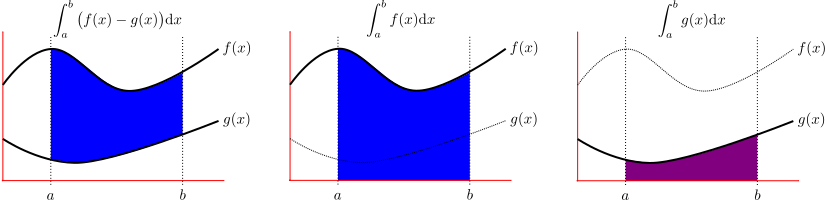
\includegraphics[width=0.9\textwidth]{area_between2}
\end{wfig}
We already know that $\int_a^b f(x)\,\dee{x}$ is the area of the region
\begin{align*}
S_2=\big\{\ (x,y)\ \big|\ a\le x\le b\,,\, 0\le y\le f(x)\ \big\}
\end{align*}
sketched in the middle figure above and that $\int_a^b g(x)\,\dee{x}$ is the area of the
region
\begin{align*}
S_3=\big\{\ (x,y)\ \big|\ a\le x\le b\,,\, 0\le y\le g(x)\ \big\}
\end{align*}
sketched in the right hand figure above. Now the region $S_1$ of the left hand figure
can be constructed by taking the region $S_2$ of center figure and removing from it the
region $S_3$ of the right hand figure. So the area of $S_1$ is exactly
\begin{align*}
  \int_a^b f(x)\,\dee{x} -  \int_a^b g(x)\,\dee{x}
  &=  \int_a^b \big(f(x)-g(x)\big)\,\dee{x}
\end{align*}
This computation depended on the assumption that $f(x)>g(x)$ and,
in particular, that the curves $y=g(x)$ and $y=f(x)$ did not cross.
If they do cross, as in this figure
\begin{efig}
 \centering
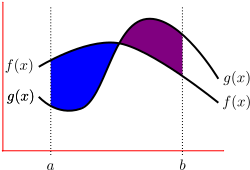
\includegraphics[height=45mm]{area_between1a}
\end{efig}
then we have to be a lot more careful. The idea is to separate the domain of
integration depending on where $f(x) - g(x)$ changes sign --- i.e. where the curves
intersect. We will illustrate this in Example~\ref{eg:AREAc} below.


Let us start with an example that makes the link to Riemann sums and definite integrals
quite explicit.
\begin{eg}\label{eg areabetween riemann}
 Find the area bounded by the curves $y=4-x^2$, $y=x$, $x=-1$ and $x=1$.

\soln
\begin{itemize}
 \item Before we do any calculus, it is a very good idea to make a sketch of the area in
question. The curves $y=x$, $x=-1$ and $x=1$ are all straight lines, while the curve
$y=4-x^2$ is a parabola whose apex is at $(0,4)$ and then curves down  (because of the
minus sign in $-x^2$) with $x$-intercepts at $(\pm2,0)$. Putting these together gives
\begin{efig}
 \centering
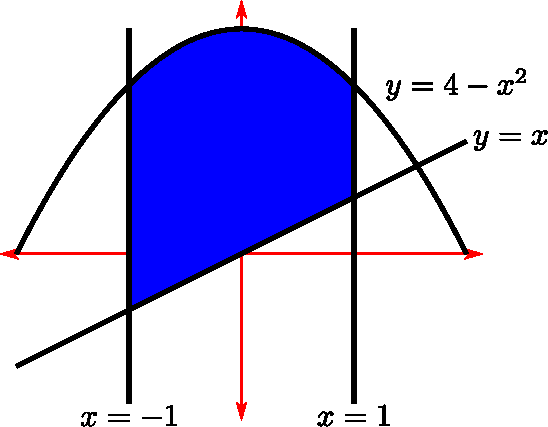
\includegraphics[height=5cm]{area_between3}
\end{efig}
Notice that the curves $y=4-x^2$ and $y=x$ intersect when $4-x^2=x$, namely when $x=
\frac{1}{2}\left(-1\pm\sqrt{17}\right) \approx 1.56,-2.56$. Hence the curve $y=4-x^2$
lies above the line $y=x$ for all $-1\le x\le 1$.

\item We are to find the area of the shaded region. Each point $(x,y)$ in this
shaded region has $-1\le x\le 1$ and $x \le y \le 4-x^2$. When we were
defining the integral (way back in Definition~\ref{def:INTintegral}) we used $a$ and $b$
to denote the smallest and largest allowed values of $x$; let's do that here too.
Let's also use $B(x)$ to denote the bottom curve (i.e. to denote the smallest allowed
value of $y$ for a given $x$) and use $T(x)$ to denote the top curve (i.e. to denote the
largest allowed value of $y$ for a given $x$). So in this example
\begin{align*}
a=-1&& b=1&& B(x)=x&& T(x)=4-x^2
\end{align*}
and the shaded region is
\begin{align*}
\big\{\ (x,y)\ \big|\ a\le x\le b,\ B(x)\le y\le T(x)\ \big\}
\end{align*}

\item We use the same strategy as we used when defining the integral in
Section~\ref{sec:defInt}:
\begin{itemize}
 \item Pick a natural number $n$ (that we will later send to infinity), then
\item subdivide the region into $n$ narrow slices, each of width $\De x=\frac{b-a}{n}$.
\item For each $i=1,2,\dots,n$, slice number $i$ runs from $x=x_{i-1}$ to $x=x_i$, and we
approximate its area by the area of a rectangle. We pick a number $x_i^*$ between
$x_{i-1}$ and $x_i$ and approximate the slice by a rectangle whose top is at $y=T(x_i^*)$
and whose bottom is at $y=B(x_i^*)$.
\item Thus the area of slice $i$ is approximately $\big[T(x_i^*)-B(x_i^*)\big]\De x$ (as
shown in the figure below).
\end{itemize}
\begin{efig}
 \centering
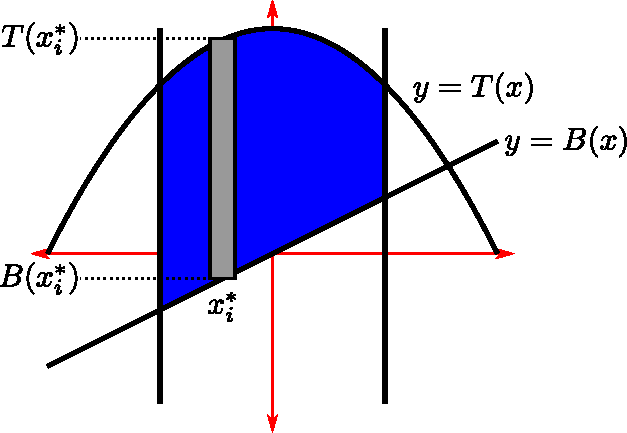
\includegraphics[height=5cm]{area_between4}
\end{efig}
\item So the Riemann sum approximation of the area is
\begin{align*}
  \text{Area} &\approx \sum_{i=1}^n  \big[T(x_i^*)-B(x_i^*)\big]\De x
\end{align*}
\item By taking the limit as $n \to \infty$ (i.e. taking the limit as the width of the
rectangles goes to zero), we convert the Riemann sum into a definite integral (see
Definition~\ref{def:INTintegral}) and at the same time our approximation of the area
becomes the exact area:
\begin{align*}
\lim_{n\rightarrow\infty}\sum_{i=1}^n  \big[T(x_i^*)-B(x_i^*)\big]\De x
&=\int_a^b \big[T(x)-B(x)\big]\dee{x} & \text{Riemann sum $\to$ integral}\\
&=\int_{-1}^1\big[(4-x^2)-x\big]\dee{x}\\
&=\int_{-1}^1\big[4-x-x^2\big]\dee{x} \\
&=\bigg[4x - \frac{x^2}{2} - \frac{x^3}{3} \bigg]_{-1}^1\\
&= \left(4 - \frac{1}{2}-\frac{1}{3} \right) - \left(-4-\frac{1}{2}+\frac{1}{3} \right)\\
&= \frac{24-3-2}{6} - \frac{-24-3+2}{6} \\
&= \frac{19}{6} + \frac{25}{6}\\
&= \frac{44}{6} = \frac{22}{3}.
\end{align*}
\end{itemize}
\end{eg}

Oof! Thankfully we generally do not need to go through the Riemann sum steps to get to
the answer. Usually, provided we are careful to check where curves intersect and which
curve lies above which, we can just jump straight to the integral
\begin{align}\label{eqn areabetween}
  \text{Area} &= \int_a^b \big[T(x)-B(x)\big]\dee{x}.
\end{align}
So let us redo the above example.
\begin{eg}[Example~\ref{eg areabetween riemann} revisited]
              \label{eg areabetween riemann again}
 Find the area bounded by the curves $y=4-x^2$, $y=x$, $x=-1$ and $x=1$.

\soln
\begin{itemize}
 \item We first sketch the region
\begin{efig}
 \centering
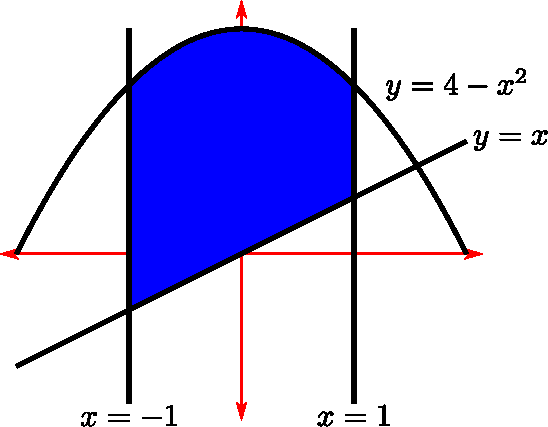
\includegraphics[height=5cm]{area_between3}
\end{efig}
and verify\footnote{We should do this by checking where the curves intersect; that is by
solving $T(x)=B(x)$ and seeing if any of the solutions lie in the range $-1\leq x \leq
1$.} that $y=T(x)=4-x^2$ lies above the curve $y=B(x)=x$ on the region $-1\leq x\leq 1$.

\item The area between the curves is then
\begin{align*}
\text{Area} &= \int_a^b \big[T(x)-B(x)\big]\dee{x}\\
&=\int_{-1}^1\big[4-x-x^2\big]\dee{x} \\
&=\bigg[4x - \frac{x^2}{2} - \frac{x^3}{3} \bigg]_{-1}^1\\
&= \frac{19}{6} + \frac{25}{6} = \frac{44}{6} = \frac{22}{3}.
\end{align*}
\end{itemize}

\end{eg}


\begin{eg}\label{eg:AREAa}
Find the area of the finite region bounded by $y=x^2$ and
$y=6x-2x^2$.

\soln This is a little different from the previous question, since we are not given
bounding lines $x=a$ and $x=b$ --- instead we have to determine the minimum and maximum
allowed values of $x$ by determining where the curves intersect. Hence our very first
task is to get a good idea of what the region looks like by sketching it.
\begin{itemize}
\item Start by sketching the region:
\begin{itemize}
\item The curve $y=x^2$ is a parabola. The point on this parabola with the
smallest $y$--coordinate is $(0,0)$. As $|x|$ increases, $y$ increases
so the parabola opens upward.

\item The curve $y=6x-2x^2 =-2(x^2-3x) =-2(x-\frac{3}{2})^2+\frac{9}{2}$ is also a
parabola. The point on this parabola with the largest value of $y$ has
$x=\nicefrac{3}{2}$
(so that the negative term in $-2(x-\frac{3}{2})^2+\frac{9}{2}$ is zero). So the point
with the largest value of $y$ is is $(\nicefrac{3}{2},\nicefrac{9}{2})$. As $x$ moves
away
from $\nicefrac{3}{2}$, either to the right or to the left, $y$ decreases. So the
parabola
opens downward. The parabola crosses the $x$--axis when $0=6x-2x^2=2x(3-x)$. That is,
when
$x=0$ and $x=3$.

\item The two parabolas intersect when $x^2= 6x-2x^2$, or
   \begin{align*}
      3x^2-6x&=0 \\
      3x(x-2)&=0
    \end{align*}
So there are two points of intersection, one being $x=0$, $y=0^2=0$
and the other being $x=2$, $y=2^2=4$.
\item The finite region between the curves lies between these two points of
intersection.
\end{itemize}
This leads us to the sketch
\begin{efig}
\begin{center}
   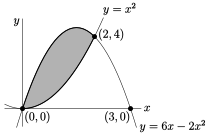
\includegraphics{areaSMPL}
\end{center}
\end{efig}
\item So on this region we have $0\leq x\leq 2$, the top curve is $T(x)=6x-2x^2$ and the
bottom curve is $B(x)=x^2$. Hence the area is given by
\begin{align*}
  \text{Area} &=\int_a^b \big[T(x)-B(x)\big]\dee{x} \\
&=\int_0^2\big[(6x-2x^2)-(x^2)\big]\dee{x}\\
&=\int_0^2\big[6x-3x^2\big]\dee{x} \\
&=\bigg[6\frac{x^2}{2}-3\frac{x^3}{3}\bigg]_0^2\\
&=3(2)^2-2^3 =4
\end{align*}


\end{itemize}

\end{eg}

\begin{eg}\label{eg:AREAb}
Find the area of the finite region bounded by $y^2=2x+6$ and
$y=x-1$.

\soln We show two different solutions to this problem. The first takes the approach
we have in  Example~\ref{eg:AREAa} but leads to messy algebra. The
second requires a little bit of thinking at the beginning but then is quite
straightforward. Before we get to that we should start by by sketching the region.
\begin{itemize}
\item The curve $y^2=2x+6$, or equivalently $x=\frac{1}{2} y^2-3$
is a parabola. The point on this parabola with the smallest $x$--coordinate
has $y=0$ (so that the positive term in $\frac{1}{2} y^2-3$ is
zero). So the point on this parabola with the smallest $x$--coordinate
is $(-3,0)$. As $|y|$ increases, $x$ increases so the parabola opens to
the right.

\item The curve $y=x-1$ is a straight line of slope $1$ that passes through
$x=1$, $y=0$.

\item The two curves intersect when $\frac{y^2}{2}-3=y+1$, or
   \begin{align*}
      y^2-6 &= 2y+2 \\
      y^2-2y-8 &= 0 \\
      (y+2)(y-4) &= 0
    \end{align*}
So there are two points of intersection, one being $y=4$, $x=4+1=5$
and the other being $y=-2$, $x=-2+1=-1$.
\item Putting this all together gives us the sketch
\begin{efig}
\begin{center}
   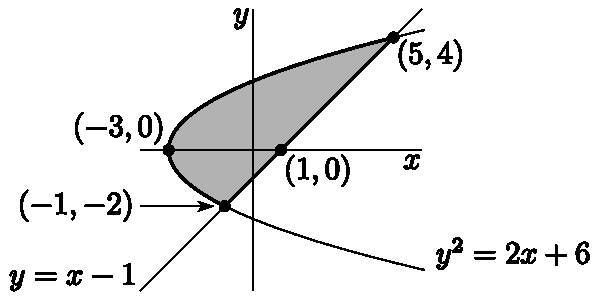
\includegraphics{areaY}
\end{center}
\end{efig}
\end{itemize}
As noted above, we can find the area of this region by approximating it by a union
of narrow vertical rectangles, as we did in Example \ref{eg:AREAa} --- though it is a
little harder. The easy way is to approximate it by a union of narrow horizontal
rectangles. Just for practice, here is the hard solution. The easy solution is after it.

\noindent\emph{Harder solution:}\\
\begin{itemize}
 \item As we have done previously, we approximate the region by a union of narrow
vertical rectangles, each of width $\De x$. Two of those rectangles are illustrated in
the sketch
\begin{efig}
\begin{center}
   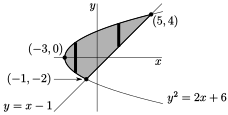
\includegraphics{areaYvert}
\end{center}
\end{efig}
\item In this region, $x$ runs from $a=-3$ to $b=5$. The curve at the top of
the region is
\begin{align*}
y&=T\big(x)=\sqrt{2x+6}
\end{align*}
The curve at the bottom of the region is more complicated. To the left of $(-1,-2)$ the
lower half of the parabola gives the bottom of the region while to the right of $(-1,-2)$
the straight line gives the bottom of the region. So
\begin{align*}
B(x)&=\begin{cases}
           -\sqrt{2x+6} & \text{if } -3\le x\le -1 \\
           x-1 & \text{if }-1\le x\le 5
      \end{cases}
\end{align*}
\item Just as before, the area is still given by the formula $\int_a^b
\big[T(x)-B(x)\big]\dee{x}$, but to accommodate our $B(x)$, we have to split
up the domain of integration when we evaluate the integral.
\begin{align*}
\int_a^b \big[T(x)-B(x)\big]\dee{x}
  &=  \int_{-3}^{-1} \big[T(x)-B(x)\big]\dee{x}
          +\int_{-1}^5 \big[T(x)-B(x)\big]\dee{x} \\
  &= \int_{-3}^{-1} \big[\sqrt{2x+6}-(-\sqrt{2x+6})\big]\dee{x}
          +\int_{-1}^5 \big[\sqrt{2x+6}-(x-1)\big]\dee{x} \\
  &= 2\int_{-3}^{-1} \sqrt{2x+6}\dee{x}
          +\int_{-1}^5 \sqrt{2x+6} - \int_{-1}^5(x-1)\dee{x}
\end{align*}
\item The third integral is straightforward, while we evaluate the first two via the
substitution rule. In particular, set $u=2x+6$ and replace $\dee{x} \rightarrow
\frac{1}{2}\dee{u}$. Also $u(-3)=0, u(-1)=4, u(5)=16$. Hence
\begin{align*}
\text{Area}
  &= 2\int_0^4\sqrt{u}\ \frac{\dee{u}}{2}
          +\int_4^{16} \sqrt{u}\ \frac{\dee{u}}{2}
          -\int_{-1}^5 (x-1)\dee{x} \\
  &= 2\bigg[\frac{ u^{\nicefrac{3}{2}} }{ \nicefrac{3}{2} }\frac{1}{2}\bigg]_0^4
 +\bigg[\frac{ u^{\nicefrac{3}{2}} }{ \nicefrac{3}{2} }\frac{1}{2}\bigg]_4^{16}
 -\bigg[\frac{x^2}{2}-x\bigg]_{-1}^5 \\[0.1in]
 & = \frac{2}{3}\big[8-0]
     +\frac{1}{3}[64-8]
     -\Big[\Big(\frac{25}{2}-5\Big)-\Big(\frac{1}{2}+1\Big)\Big] \\[0.1in]
 & = \frac{72}{3} -\frac{24}{2}+6 \\
&=18
\end{align*}
Oof!
\end{itemize}
\medskip\noindent\emph{Easier solution:}\\
The easy way to determine the area of our region is to approximate by narrow
horizontal rectangles, rather than narrow vertical rectangles. (Really we are just
swapping the roles of $x$ and $y$ in this problem)
\begin{itemize}
\item Look at our sketch of the region again --- each point $(x,y)$ in our
region has $-2\le y\le 4$ and $\frac{1}{2}(y^2-6)\le x \le y+1$.
\item Let's use
\begin{itemize}
\item
$c$ to denote the smallest allowed value of $y$,
\item
$d$ to denote the largest allowed value of $y$
\item
$L(y)$ (``$L$'' stands for ``left'') to denote the smallest allowed
value of $x$, when the $y$--coordinate is $y$, and
\item
$R(y)$ (``$R$'' stands for ``right'') to denote the largest allowed value
of $x$, when the $y$--coordinate is $y$.
\end{itemize}
So, in this example,
\begin{align*}
c=-2&& d=4 &&  L(y)=\frac{1}{2}(y^2-6) && R(y)=y+1
\end{align*}
and the shaded region is
\begin{align*}
\big\{\ (x,y)\ \big|\ c\le y\le d,\ L(y)\le x\le R(y)\ \big\}
\end{align*}
\item Our strategy is now nearly the same as that used in Example~\ref{eg areabetween
riemann}:
\begin{itemize}
 \item Pick a natural number $n$ (that we will later send to infinity), then
 \item subdivide the interval $c\le y\le d$ into $n$ narrow subintervals, each of width
$\De y=\frac{d-c}{n}$. Each subinterval cuts a thin horizontal slice from the region (see
the figure below).
 \item We approximate the area of slice number $i$ by the area of a thin
horizontal rectangle (indicated by the dark rectangle in the figure below). On this
slice, the $y$--coordinate runs over a very narrow range.
We pick a number $y_i^*$, somewhere in that range. We approximate slice
$i$ by a rectangle whose left side is at $x=L(y_i^*)$ and whose right side
is at $x=R(y_i^*)$.
\item Thus the area of slice $i$ is approximately $\big[R(x_i^*)-L(x_i^*)\big]\De y$.
\end{itemize}
\begin{efig}
\begin{center}
   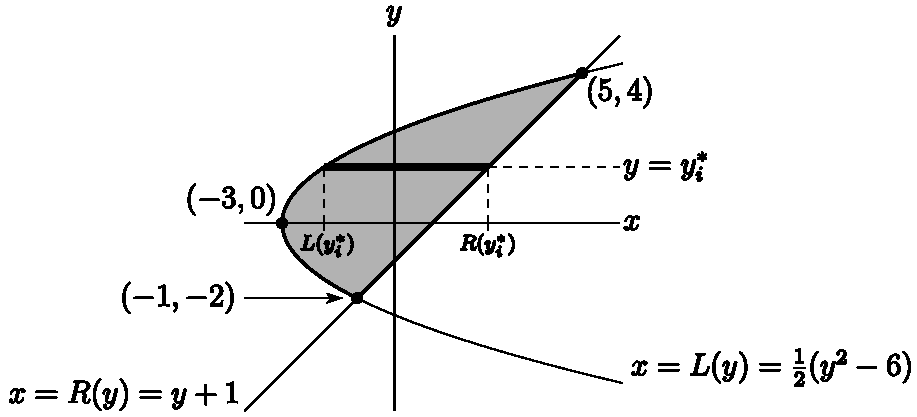
\includegraphics{areaYhor}
\end{center}
\end{efig}
\item The desired area is
\begin{align*}
\lim_{n\rightarrow\infty}\sum_{i=1}^n \big[R(y_i^*)-L(y_i^*)\big]\De y
&=\int_c^d \big[R(y)-L(y)\big]\dee{y} & \text{Riemann sum $\rightarrow$ integral}\\
&=\int_{-2}^4 \big[(y+1)-\tfrac{1}{2}\big(y^2-6\big)\big]\dee{y} \\
&=\int_{-2}^4 \big[-\tfrac{1}{2}y^2+y+4\big]\dee{y} \\
&=\Big[-\tfrac{1}{6}y^3+\tfrac{1}{2}y^2+4y\Big]_{-2}^4 \\
&=-\tfrac{1}{6}\big(64-(-8)\big)+\tfrac{1}{2}(16-4)+4(4+2)\\
&=-12+6+24 \\
&=18
\end{align*}
\end{itemize}

\end{eg}

One last example.
\begin{eg}\label{eg:AREAc}
Find the area between the curves $y=\dfrac{1}{\sqrt{2}}$ and $y=\sin(x)$ with $x$ running
from $0$ to $\nicefrac{\pi}{2}$.

\soln This one is a little trickier since (as we shall see) the region is split into two
pieces and we need to treat them separately.

\begin{itemize}
 \item Again we start by sketching the region.
\begin{efig}
\begin{center}
   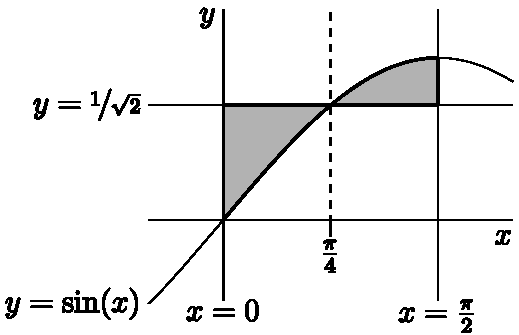
\includegraphics{areaCross}
\end{center}
\end{efig}
We want the shaded area.
\item Unlike our previous examples, the bounding curves $y=\nicefrac{1}{\sqrt{2}}$ and
$y=\sin(x)$ cross in the middle of the region of interest. They cross when
$y=\nicefrac{1}{\sqrt{2}}$ and $\sin(x)=y=\nicefrac{1}{\sqrt{2}}$, i.e. when
$x=\nicefrac{\pi}{4}$. So
\begin{itemize}
\item to the left of $x=\nicefrac{\pi}{4}$, the top boundary is part of the straight line
$y=\nicefrac{1}{\sqrt{2}}$ and  the bottom boundary is part of the curve $y=\sin(x)$
\end{itemize}
\begin{itemize}
\item while to the right of $x=\nicefrac{\pi}{4}$, the top boundary is part of the curve
$y=\sin(x)$ and the bottom boundary is part of the straight line
$y=\nicefrac{1}{\sqrt{2}}$.
\end{itemize}
\item Thus the formulae for the top and bottom boundaries are
\begin{align*}
T(x)=\left.\begin{cases}
          \nicefrac{1}{\sqrt{2}} & \text{if $0\le x\le \nicefrac{\pi}{4}$}\\
          \sin(x)& \text{if $\nicefrac{\pi}{4}\le x\le \nicefrac{\pi}{2}$}
      \end{cases}\right\}\qquad
B(x)=\left.\begin{cases}
          \sin(x) & \text{if $0\le x\le \nicefrac{\pi}{4}$}\\
          \nicefrac{1}{\sqrt{2}}& \text{if $\nicefrac{\pi}{4}\le x\le \nicefrac{\pi}{2}$}
      \end{cases}\right\}
\end{align*}
We may compute the area of interest using our canned formula
\begin{align*}
\text{Area} = \int_a^b \big[T(x)-B(x)\big]\dee{x}
\end{align*}
but since the formulas for $T(x)$ and $B(x)$ change at the point $x=\nicefrac{\pi}{4}$,
we must split the domain of the integral in two at that point\footnote{We are
effectively computing the area of the region by computing the area of the two disjoint
pieces separately. Alternatively, if we set $f(x) = \sin(x)$ and $g(x)
=\nicefrac{1}{\sqrt{2}}$, we can rewrite the integral $\int_a^b \big[T(x) -
B(x)\big]\,\dee{x}$ as $\int_a^b \big|f(x) - g(x)\big|\,\dee{x}$. To see that the two
integrals are the same, split the domain of integration where $f(x)-g(x)$ changes sign.}

\item Our integral over the domain $0\leq x \leq \nicefrac{\pi}{2}$ is split into an
integral over $0\le x\le \nicefrac{\pi}{4}$ and one over $\nicefrac{\pi}{4}\le x\le
\nicefrac{\pi}{2}$:
\begin{align*}
\text{Area} &= \int_0^{\nicefrac{\pi}{2}} \big[T(x)-B(x)\big]\dee{x} \\
   &= \int_0^{\nicefrac{\pi}{4}} \big[T(x)-B(x)\big]\dee{x}
      +\int_{\nicefrac{\pi}{4}}^{\nicefrac{\pi}{2}} \big[T(x)-B(x)\big]\dee{x} \\
   &= \int_0^{\nicefrac{\pi}{4}} \Big[\frac{1}{\sqrt{2}}-\sin(x)\Big]\dee{x}
      +\int_{\nicefrac{\pi}{4}}^{\nicefrac{\pi}{2}}
                       \Big[\sin(x)-\frac{1}{\sqrt{2}}\Big]\dee{x} \\[0.1in]
   &= \Big[\frac{x}{\sqrt{2}}+\cos(x)\Big]_0^{\nicefrac{\pi}{4}}
      +\Big[-\cos(x)-\frac{x}{\sqrt{2}}\Big]
                _{\nicefrac{\pi}{4}}^{\nicefrac{\pi}{2}}  \\[0.1in]
   &= \Big[\frac{1}{\sqrt{2}}\frac{\pi}{4}+\frac{1}{\sqrt{2}}-1\Big]
      +\Big[\frac{1}{\sqrt{2}}-\frac{1}{\sqrt{2}}\frac{\pi}{4}\Big]  \\[0.1in]
  &=\frac{2}{\sqrt{2}}-1 \\[0.1in]
  &=\sqrt{2}-1
\end{align*}

\end{itemize}

\end{eg}

% \begin{comment}
\section{Volumes}\label{sec int volumes}
Another simple\footnote{Well --- arguably the idea isn't too complicated and is a
continuation of the idea used to compute areas in the previous section. In practice this
can be quite tricky as we shall see.} application of integration is computing volumes. We
use the same strategy as we used to express areas of regions in two
dimensions as integrals --- approximate the region by a union of small,
simple pieces whose volume we can compute and then then take the limit
as the ``piece size'' tends to zero.

In many cases this will lead to ``multivariable integrals'' that are beyond our present
scope\footnote{Typically such integrals (and more) are covered in a third calculus
course.}. But there are some special cases in which this leads to integrals that we
can handle. Here are some examples.

\begin{eg}[Cone]\label{eg:VOLa}
Find the volume of the circular cone of height $h$ and radius $r$.

\soln Here is a sketch of the cone.
\vadjust{
\begin{efig}
\begin{center}
   \includegraphics{cone}
\end{center}
\end{efig}
}
We have called the vertical axis $x$, just so that we end up with a ``$\dee{x}$''
integral.

\begin{itemize}
 \item In what follows we will slice the cone into thin horizontal ``pancakes''. In order
to approximate the volume of those slices, we need to know the radius of the cone at a
height $x$ above its point. Consider the cross sections shown in the following figure.
\begin{efig}
\begin{center}
   \includegraphics[width=0.7\textwidth]{cone_adr1}
\end{center}
\end{efig}
At full height $h$, the cone has radius $r$. If we cut the cone at height $x$, then by
similar triangles (see the figure on the right) the radius will be $\frac{x}{h}\cdot r$.


\item Now think of cutting the cone into $n$ thin horizontal ``pancakes''. Each such
pancake is approximately a squat cylinder of height $\De x=\nicefrac{h}{n}$. This
is very similar to how we approximated the area under a curve by $n$ tall thin
rectangles. Just as we approximated the area under the curve by summing these rectangles,
we can approximate the volume of the cone by summing the volumes of these cylinders. Here
is a side view of the cone and one of the cylinders.
\begin{efig}
\begin{center}
   \includegraphics[width=0.85\textwidth]{cone_adr2}
\end{center}
\end{efig}

\item We follow the method we used in Example~\ref{eg areabetween riemann}, except that
our slices are now pancakes instead of rectangles.
\begin{itemize}
 \item Pick a natural number $n$ (that we will later send to infinity), then
\item subdivide the cone into $n$ thin pancakes, each of width $\De
x=\frac{h}{n}$.
\item For each $i=1,2,\dots,n$, pancake number $i$ runs from
$x=x_{i-1}=(i-1)\cdot\De x$ to $x=x_i=i\cdot\De x$, and we approximate its
volume by the volume of a squat cone. We pick a number $x_i^*$ between $x_{i-1}$ and
$x_i$
and approximate the pancake by a cylinder of height $\De x$ and radius $\frac{x_i^*}{h}r$.
  \item Thus the volume of pancake $i$ is
approximately $\pi \left( \frac{x_i^*}{h}r\right)^2 \De x$ (as shown in the figure above).
\end{itemize}

\item So the Riemann sum approximation of the volume is
\begin{align*}
  \text{Volume} &\approx \sum_{i=1}^n  \pi \left( \frac{x_i^*}{h}r\right)^2 \De x
\end{align*}
\item By taking the limit as $n \to \infty$ (i.e. taking the limit as the thickness of
the pancakes goes to zero), we convert the Riemann sum into a definite integral (see
Definition~\ref{def:INTintegral}) and at the same time our approximation of the volume
becomes the exact volume:
\begin{align*}
\int_0^h \pi \Big(\frac{x}{h}r\Big)^2\dee{x}
\end{align*}
\end{itemize}
Our life\footnote{At least the bits of it involving integrals.} would be easier if
we could avoid all this formal work with Riemann sums every time we encounter a new
volume. So before we compute the above integral, let us redo the above calculation in a
less formal manner.
\begin{itemize}
 \item Start again from the picture of the cone
\vadjust{
\begin{efig}
\begin{center}
   \includegraphics{cone}
\end{center}
\end{efig}
}
and think of slicing it into thin pancakes, each of width $\dee{x}$.
\vadjust{
\begin{efig}
\begin{center}
   \includegraphics{coneX}\qquad\includegraphics{coneT}
\end{center}
\end{efig}
}
\item The pancake at height $x$ above the point of the cone (which is the fraction
$\frac{x}{h}$ of the total height of the cone) has
\begin{itemize}
\item radius $\frac{x}{h}\cdot r$ (the fraction $\frac{x}{h}$ of the
full radius, $r$) and so
\item cross--sectional area $\pi \big(\frac{x}{h}r\big)^2$,
\item thickness $\dee{x}$ --- we have done something a little sneaky here, see the
discussion below.
\item volume $\pi \big(\frac{x}{h}r\big)^2\dee{x}$
\end{itemize}
As $x$ runs from $0$ to $h$, the total volume is
\begin{align*}
\int_0^h \pi \Big(\frac{x}{h}r\Big)^2\dee{x}
&=\frac{\pi r^2}{h^2}\int_0^h x^2\dee{x}\\
&=\frac{\pi r^2}{h^2} \bigg[\frac{x^3}{3}\bigg]_0^h\\
&=\frac{1}{3}\pi r^2 h
\end{align*}
\end{itemize}
In this second computation we are using a time-saving trick. As we saw in
the formal computation above, what we really need to do is pick a natural number $n$,
slice the cone into $n$ pancakes each of thickness $\De x = \nicefrac{h}{n}$ and then
take the limit as $n \to \infty$. This led to the Riemann sum
\begin{align*}
  \sum_{i=1}^n \pi \left( \frac{x_i^*}{h} r \right)^2 \De x && \text{which becomes}
  \int_0^h \pi \left( \frac{x}{h} r \right)^2 \dee{x}
\end{align*}
So knowing that we will replace
\begin{align*}
  \sum_{i=1}^n &\longrightarrow \int_0^h\\
  x_i^* &\longrightarrow x\\
  \De x &\longrightarrow \dee{x}
\end{align*}
when we take the limit, we have just skipped the intermediate steps. While this is not
entirely rigorous, it can be made so, and does save us a lot of algebra.
\end{eg}

\goodbreak
\begin{eg}[Sphere]\label{eg:VOLs}
Find the volume of the sphere of radius $r$.

\soln We'll find the volume of the part of the sphere in the first octant\footnote{The
first octant is the set of all points $(x,y,z)$ with $x\ge 0$, $y\ge 0$ and $z\ge 0$.},
sketched below. Then we'll multiply by $8$.

\begin{itemize}
 \item To compute the volume,
\vadjust{
\begin{efig}
\begin{center}
   \includegraphics{sphereSlice}
\end{center}
\end{efig}
}%
we slice it up into thin vertical ``pancakes'' (just as we did in the previous example).

\item Each pancake is one quarter of a thin circular disk. The pancake a distance $x$
from the $yz$--plane is shown in the sketch above. The radius of that pancake is the
distance from the dot shown in the figure to the $x$--axis, i.e. the $y$--coordinate
of the dot. To get the coordinates of the dot, observe that
\begin{itemize}
\item it lies the $xy$--plane, and so has $z$--coordinate zero,
and that
\item it also lies on the sphere, so that its coordinates obey
$x^2+y^2+z^2=r^2$. Since $z=0$ and $y>0$, $y=\sqrt{r^2-x^2}$.
\end{itemize}
\item So the pancake at distance $x$ from the $yz$--plane has
\begin{itemize}
\item thickness\footnote{Yet again what we really do is pick a natural
number $n$, slice the octant of the sphere into $n$ pancakes each of thickness
$\De x=\frac{r}{n}$ and then take the limit $n\rightarrow\infty$.
In the integral $\De x$ is replaced by $\dee{x}$. Knowing that this is what
is going to happen, we again just skip a few steps.} $\dee{x}$ and
\item
radius $\sqrt{r^2-x^2}$
\item cross--sectional area $\frac{1}{4}\pi \big(\sqrt{r^2-x^2}\,\big)^2$
and hence
\item
volume $\frac{\pi}{4} \big(r^2-x^2\big)\dee{x}$
\end{itemize}
\item As $x$ runs from $0$ to $r$, the total volume of the part of the sphere
in the first octant is
\begin{align*}
\int_0^r \frac{\pi}{4} \big(r^2-x^2\big)\dee{x}
=\frac{\pi}{4}\bigg[r^2x-\frac{x^3}{3}\bigg]_0^r
=\frac{1}{6}\pi r^3
\end{align*}
and the total volume of the whole sphere is eight times that, which is
$\frac{4}{3}\pi r^3$, as expected.
\end{itemize}
\end{eg}


\begin{eg}[Revolving a region]\label{eg:VOLe}
The region between the lines $y=3$, $y=5$, $x=0$ and $x=4$
is rotated around the line $y=2$. Find the volume of the region
swept out.

\soln As with most of these problems, we should start by sketching the problem.
\begin{efig}
\begin{center}
   \includegraphics{revolveA}
\end{center}
\end{efig}
\begin{itemize}
 \item Consider the region and slice it into thin vertical strips of width
$\dee{x}$.
\item  Now we are to rotate this region about the line $y=2$. Imagine looking
straight down the axis of rotation, $y=2$, end on. The symbol in the figure
above just to the right of the end the line $y=2$ is supposed to represent your
eye\footnote{Okay okay\dots We missed the pupil. I'm sure there is a pun in
there somewhere.}. Here is what you see as the rotation takes place.
\begin{efig}
\begin{center}
   \includegraphics{revolveB}
\end{center}
\end{efig}
\item Upon rotation about the line $y=2$ our strip sweeps out a ``washer''
\begin{itemize}
\item
whose cross--section is a disk of radius $5-2=3$ from which
a disk of radius $3-2=1$ has been removed so that it has a
\item
cross--sectional area of $\pi 3^2 -\pi 1^2 = 8\pi$ and a
\item
thickness $\dee{x}$ and hence a
\item
volume $8\pi\,\dee{x}$.
\end{itemize}
\item As our leftmost strip is at $x=0$ and our rightmost strip is
at $x=4$, the total
\begin{align*}
\text{Volume}
&= \int _0^4 8\pi\,\dee{x}
=(8\pi)(4)
=32\pi
\end{align*}
\end{itemize}
Notice that we could also reach this answer by writing the volume as the
difference of two cylinders.
\begin{itemize}
 \item The outer cylinder has radius $(5-2)$ and length 4. This has volume
\begin{align*}
  V_{outer} &= \pi r^2 \ell = \pi \cdot 3^2 \cdot 4 = 36\pi.
\end{align*}
 \item The inner cylinder has radius $(3-2)$ and length 4. This has volume
\begin{align*}
  V_{inner} &= \pi r^2 \ell = \pi \cdot 1^2 \cdot 4 = 4\pi.
\end{align*}
\item The volume we want is the difference of these two, namely
\begin{align*}
  V &= V_{outer} - V_{inner} = 32\pi.
\end{align*}
\end{itemize}

\end{eg}

Let us turn up the difficulty a little on this last example.
\begin{eg}[Revolving again]\label{eg rot xaxis}
The region between the curve $y=\sqrt{x}$, and the lines $y=0$, $x=0$ and $x=4$
is rotated around the line $y=0$. Find the volume of the region swept out.

\soln We can approach this in much the same way as the previous example.
\begin{itemize}
 \item Consider the region and cut it into thin vertical strips of width $\dee{x}$.
\begin{efig}
 \centering
\includegraphics[height=45mm]{rot_rootx1}
\end{efig}

\item When we rotate the region about the line $y=0$, each strip sweeps out a thin
pancake
\begin{itemize}
\item
whose cross-section is a disk of radius $\sqrt{x}$ with a
\item
cross-sectional area of $\pi (\sqrt{x})^2 = \pi x$ and a
\item
thickness $\dee{x}$ and hence a
\item
volume $\pi x \dee{x}$.
\end{itemize}
\item As our leftmost strip is at $x=0$ and our rightmost strip is
at $x=4$, the total
\begin{align*}
\text{Volume}
&= \int _0^4 \pi x \dee{x}
=\left[\frac{\pi}{2}x^2 \right]_0^4
=8\pi
\end{align*}
\end{itemize}

\end{eg}
In the last example we considered rotating a region around the $x$-axis. Let us do the
same but rotating around the $y$-axis.
\begin{eg}[Revolving yet again]\label{eg rot yaxis}
The region between the curve $y=\sqrt{x}$, and the lines $y=0$, $x=0$ and $x=4$
is rotated around the line $x=0$. Find the volume of the region swept out.

\soln
\begin{itemize}
 \item We will cut the region into horizontal slices, so we should write $x$ as a
function of $y$. That is, the region is bounded by $x=y^2$, $x=4$, $y=0$ and $y=2$.
 \item Now slice the region into thin horizontal strips of width $\dee{y}$.
\begin{wfig}
 \centering
\includegraphics[width=0.95\textwidth]{rot_rootx3}
\end{wfig}

\item When we rotate the region about $y$-axis, each strip sweeps out a thin
washer
\begin{itemize}
\item whose inner radius is $y^2$ and outer radius is $4$, and
\item thickness is $\dee{y}$ and hence
\item has volume $\pi(r_{out}^2 - r_{in}^2)\dee{y} = \pi(16-y^4)\dee{y}$.
\end{itemize}
\item As our bottommost strip is at $y=0$ and our topmost
strip is at $y=2$, the total
\begin{align*}
\text{Volume}
&= \int _0^2 \pi(16-y^4) \dee{y}
=\left[16\pi y - \frac{\pi}{5}y^5 \right]_0^2
= 32\pi - \frac{32\pi}{5} = \frac{128\pi}{5}.
\end{align*}
\end{itemize}
\end{eg}
There is another way\footnote{The method is not a core part of the course and should be
considered optional.} to do this one which we show at the end of this section.


\begin{eg}[Pyramid]\label{eg:VOLb}
Find the volume of the pyramid which has height $h$ and whose base is a
square of side $b$.

\soln Here is a sketch of the part of the pyramid that is in the
first octant; we display only this portion to make the diagrams simpler.
\vadjust{
\begin{efig}
\begin{center}
   \includegraphics{pyramid}\quad\includegraphics{pyramidYZ}
\end{center}
\end{efig}
}
Note that this diagram shows only 1 quarter of the whole pyramid.

\begin{itemize}
 \item To compute its volume, we slice it up into thin horizontal ``square pancakes''. A
typical pancake also appears in the sketch above.


\begin{itemize}
\item The pancake at height $z$ is the fraction $\frac{h-z}{h}$ of the distance from the
peak of the pyramid to its base.
\item So the \emph{full} pancake\footnote{Note that this is the full pancake, not just
the part in the first octant.} at height $z$ is a square of side $\frac{h-z}{h}b$. As a
check, note that when $z=h$ the pancake has side  $\frac{h-h}{h}b=0$, and when $z=0$ the
pancake has side  $\frac{h-0}{h}b=b$.
\item So the pancake has cross-sectional area $\big(\frac{h-z}{h}b\big)^2$ and
thickness\footnote{We are again using our Riemann sum avoiding trick.} $\dee{z}$ and
hence
\item volume $\big(\frac{h-z}{h}b\big)^2\dee{z}$.
\end{itemize}
\item The volume of the whole pyramid (not just the part of the pyramid in the first
octant) is
\begin{align*}
\int_0^h \Big(\frac{h-z}{h}b\Big)^2\dee{z}
&=\frac{b^2}{h^2} \int_0^h (h-z)^2\dee{z} \\
&=\frac{b^2}{h^2} \int_h^0 -t^2\dee{t} & \text{substitution rule with
$t=(h-z), \dee{z}\to-\dee{t}$} \\
&=-\frac{b^2}{h^2}\bigg[\frac{t^3}{3}\bigg]_h^0\\
&=-\frac{b^2}{h^2}\bigg[-\frac{h^3}{3}\bigg] \\
&=\frac{1}{3} b^2h
\end{align*}

\end{itemize}

\end{eg}

Let's ramp up the difficulty a little.
\begin{eg}[Napkin Ring]\label{eg:VOLc}
Suppose you make two napkin rings\footnote{Handy things to have (when combined with cloth
napkins) if your parents are coming to dinner and you want to convince them that you are
``taking care of yourself''.} by drilling holes with different diameters through two
wooden balls. One ball has radius $r$ and the other radius $R$ with $r<R$. You
choose the diameter of the holes so that both napkin rings have the same
height, $2h$. See the
figure below.
\begin{efig}
\begin{center}
   \includegraphics{napkin}
\end{center}
\end{efig}
Which\footnote{A good question to ask to distract your parents from the fact you are
serving frozen burritos.} ring has more wood in it?

\soln We'll compute the volume of the napkin ring with radius $R$.
We can then obtain the volume of the napkin ring of radius $r$, by just replacing $R
\mapsto r$ in the result.

\begin{itemize}
 \item To compute the volume of the napkin ring of radius $R$, we slice it up into thin
horizontal ``pancakes''. Here is a sketch
of the part of the napkin ring in the first octant showing a typical
pancake.%
\vadjust{
\begin{efig}
\begin{center}
   \includegraphics{napkinRing}
\end{center}
\end{efig}
}
\item The coordinates of the two points marked in the $yz$--plane of that figure
are found by remembering that
\begin{itemize}\itemsep1pt \parskip0pt \parsep0pt
\item the equation of the sphere is $x^2+y^2+z^2=R^2$.
\item The two points have $y>0$ and are in the $yz$--plane, so that
$x=0$ for them. So $y=\sqrt{R^2-z^2}$.
\item In particular, at the top of the napkin ring $z=h$,
so that $y=\sqrt{R^2-h^2}$.
\end{itemize}
\item The pancake at height $z$, shown in the sketch, is a ``washer'' --- a circular disk
with a circular hole cut in its center.
\begin{itemize}
\item The outer radius of the washer is $\sqrt{R^2-z^2}$ and
\item the inner radius of the washer is $\sqrt{R^2-h^2}$. So the
\item  cross--sectional area of the washer is
\begin{align*}
\pi\big(\sqrt{R^2-z^2}\,\big)^2-\pi\big(\sqrt{R^2-h^2}\,\big)^2
=\pi(h^2-z^2)
\end{align*}
\end{itemize}
\item The pancake at height $z$
\begin{itemize}
\item has thickness $dz$ and
\item cross--sectional area $\pi(h^2-z^2)$ and hence
\item volume $\pi(h^2-z^2)\dee{z}$.
\end{itemize}
\item Since $z$ runs from $-h$ to $+h$, the total volume
of wood in the napkin ring of radius $R$ is
\begin{align*}
\int_{-h}^h \pi(h^2-z^2)\dee{z}
&=\pi\Big[h^2z-\frac{z^3}{3}\Big]_{-h}^h \\
&=\pi\Big[\Big(h^3-\frac{h^3}{3}\Big)
          -\Big((-h)^3-\frac{(-h)^3}{3}\Big)\Big]\\
&=\pi\Big[\frac{2}{3}h^3-\frac{2}{3}\big(-h\big)^3\Big] \\
&=\frac{4\pi}{3}h^3
\end{align*}
\end{itemize}
This volume is independent of $R$. Hence the napkin ring of radius $r$ contains precisely
the same volume of wood as the napkin ring of radius $R$!
\end{eg}

\begin{eg}[Notch]\label{eg:VOLd}
A $45^\circ$ notch is cut to the centre of a cylindrical
log having radius $20$cm. One plane face of the notch is perpendicular to
the axis of the log. See the sketch below. What volume of wood was
removed?
\begin{efig}
\begin{center}
   \includegraphics{notch2}\qquad
   \includegraphics{notch4a}\qquad
   \includegraphics{notch5a}
\end{center}
\end{efig}

\soln We show two solutions to this problem which are of comparable difficulty. The
difference lies in the shape of the pancakes we use to slice up the volume. In solution~1
we cut rectangular pancakes parallel to the $yz$--plane and in solution~2 we slice
triangular pancakes parallel to the $xz$--plane.\\

\noindent\emph{Solution 1:}
\begin{itemize}
 \item Concentrate on the notch. Rotate it around so that the plane face lies in the
$xy$--plane.
\item Then slice the notch into vertical rectangles (parallel to the $yz$--plane) as in
the figure on the left below.
\begin{efig}
\begin{center}
   \includegraphics{notch2a}\qquad
   \includegraphics[scale=0.9]{notchXZa}
\end{center}
\end{efig}
\item The cylindrical log had radius $20$cm. So the circular part of the boundary of the
base of the notch has equation $x^2+y^2=20^2$. (We're putting the origin of the
$xy$--plane at the centre of the circle.) If our coordinate system is such that $x$ is
constant on each slice, then
\begin{itemize}
\item
the base of the slice is the line segment from $(x,-y,0)$ to
$(x,+y,0)$ where  $y=\sqrt{20^2-x^2}$ so that
\item
the slice has width $2y=2\sqrt{20^2-x^2}$ and
\item
height $x$ (since the upper face of the notch is at $45^\circ$ to the base
--- see the side view sketched in the figure on the right above).
\item
So the slice has cross--sectional area $2x\sqrt{20^2-x^2}$.
\end{itemize}
\item On the base of the notch $x$ runs from $0$ to $20$ so
the volume of the notch is
\begin{align*}
V&=\int_0^{20}2x\sqrt{20^2-x^2}\dee{x}
\intertext{Make the change of variables $u=20^2-x^2$ (don't forget to change $\dee{x}
\rightarrow -\frac{1}{2x}\dee{u}$):}
V&=\int_{20^2}^{0}-\sqrt{u}\,\dee{u}\\
&=\left[-\frac{u^{3/2}}{3/2}\right]_{20^2}^0\\
&= \frac{2}{3}20^3=\frac{16,000}{3}
\end{align*}
\end{itemize}

\noindent\emph{Solution 2:}\\
\begin{itemize}
 \item  Concentrate of the notch. Rotate it around so that its base
lies in the $xy$--plane with the skinny edge along the $y$--axis.
\item Slice the notch into triangles parallel to the $xz$--plane as in the figure
on the left below. In the figure below, the triangle happens to lie in a plane
where $y$ is negative.
\begin{efig}
\begin{center}
   \includegraphics{notch3a}\qquad
   \includegraphics[scale=0.9]{notchXZb}
\end{center}

\end{efig}
\item The cylindrical log had radius $20$cm. So the circular part of the boundary of the
base of the notch has equation $x^2+y^2=20^2$. Our coordinate system is such that $y$ is
constant on each slice, so that
\begin{itemize}
\item
the base of the triangle is the line segment from $(0,y,0)$ to $(x,y,0)$ where
$x=\sqrt{20^2-y^2}$ so that
\item
the triangle has base $x=\sqrt{20^2-y^2}$  and
\item
height $x=\sqrt{20^2-y^2}$ (since the upper face of the notch is at
$45^\circ$ to the base --- see the side view sketched in the figure
on the right above).
\item
So the slice has cross--sectional area $\half\big(\sqrt{20^2-y^2}\big)^2$.
\end{itemize}
\item On the base of the notch $y$ runs from $-20$ to $20$,
so the volume of the notch is
\begin{align*}
V&=\half\int_{-20}^{20}(20^2-y^2)\dee{y}\\
&=\int_0^{20} (20^2-y^2)\dee{y}\\
&=\Big[20^2y-\frac{y^3}{3}\Big]_0^{20} \\
&=\frac{2}{3}20^3=\frac{16,000}{3}
\end{align*}
\end{itemize}
\end{eg}


\subsection*{Optional --- Cylindrical Shells}
Let us return to Example~\ref{eg rot yaxis} in which we rotate a region around the
$y$-axis. Here we show another solution to this problem which is obtained by slicing the
region into vertical strips. When rotated about the $y$-axis, each such strip sweeps out
a thin cylindrical shell. Hence the name of this approach (and this subsection).

\begin{eg}[Revolving yet again]
The region between the curve $y=\sqrt{x}$, and the lines $y=0$, $x=0$ and $x=4$
is rotated around the line $x=0$. Find the volume of the region swept out.

\soln
\begin{itemize}
 \item Consider the region and cut it into thin vertical strips of width $\dee{x}$.
\begin{efig}
 \centering
\includegraphics[height=45mm]{rot_rootx2}
\end{efig}

\item When we rotate the region about the $y$-axis, each strip sweeps out a thin
cylindrical shell
\begin{itemize}
\item whose radius is $x$,
\item height is $\sqrt{x}$, and
\item thickness is $\dee{x}$ and hence
\item has volume $2 \pi \times \text{radius} \times \text{height} \times \text{thickness}
= 2 \pi x^{3/2} \dee{x}$.
\end{itemize}
\item As our leftmost strip is at $x=0$ and our rightmost strip is
at $x=4$, the total
\begin{align*}
\text{Volume}
&= \int _0^4 2\pi x^{3/2} \dee{x}
=\left[\frac{4\pi}{5} x^{5/2} \right]_0^4
= \frac{4\pi}{5}\cdot 32 = \frac{128\pi}{5}
\end{align*}
which (thankfully) agrees with our previous computation.

\end{itemize}
\end{eg}

\section{Integration by Parts}\label{sec intbyparts}
The fundamental theorem of calculus tells us that it is very easy to integrate a
derivative. In particular, we know that
\begin{align*}
  \int \diff{}{x}\left( F(x) \right) \dee{x} &= F(x)+C
\end{align*}
We can exploit this in order to develop another rule for integration --- in particular a
rule to help us integrate products of simpler function such as
\begin{align*}
  \int x e^x \dee{x}
\end{align*}
In so doing we will arrive at a method called ``integration by parts''.


To do this we start with the product rule and integrate. Recall that the
product rule says
\begin{align*}
\diff{}{x} u(x)v(x) = u'(x)\,v(x)+u(x)\,v'(x)
\end{align*}
Integrating this gives
\begin{align*}
\int \big[u'(x)\,v(x)+u(x)\,v'(x)\big]\dee{x}
&=\big[\text{a function whose derivative is $u'v+uv'$}\big] + C \\
&=u(x)v(x) +C
\end{align*}
Now this, by itself, is not terribly useful. In order to apply it we need to have a
function whose integrand is a sum of products that is in exactly this form $u'(x)v(x) +
u(x)v'(x)$. This is far too specialised.

However if we tease this apart a little:
\begin{align*}
\int \big[ u'(x)\,v(x) + u(x)\,v'(x) \big]\dee{x}
         &=  \int u'(x)\,v(x) \,\dee{x}
           +\int u(x)\,v'(x) \,\dee{x}
\intertext{Bring one of the integrals to the left-hand side}
  u(x) v(x) - \int u'(x)\,v(x) \dee{x}
&= \int u(x)\,v'(x)\dee{x}
\intertext{Swap left and right sides}
\int u(x)\,v'(x)\dee{x}
 &= u(x) v(x) - \int u'(x)\,v(x) \dee{x}
\end{align*}
In this form we take the integral of one product and express it in terms of the integral
of a different product. If we express it like that, it doesn't seem too useful. However,
if the second integral is easier, then this process helps us.

Let us do a simple example before explaining this more generally.
\begin{eg}[$\int xe^x \dee{x}$]\label{eg:PRTSxex}
Compute the integral $\ds \int xe^x \dee{x}$.

\soln
\begin{itemize}
 \item We start by taking the equation above
\begin{align*}
 \int u(x)\,v'(x)\dee{x}
 &= u(x) v(x) - \int u'(x)\,v(x) \dee{x}
\end{align*}
 \item Now set $u(x)=x$ and $v'(x)=e^x$. How did we know how to make this choice? We will
explain some strategies later. For now, let us just accept this choice and keep going.
\item In order to use the formula we need to know $u'(x)$ and $v(x)$. In this case it is
quite straightforward: $u'(x)=1$ and $v(x)=e^x$.
\item Plug everything into the formula:
\begin{align*}
  \int x e^x \dee{x} &= x e^x - \int e^x \dee{x}
\intertext{So our original more difficult integral has been turned into a question of
computing an easy one.}
&= x e^x - e^x +C
\end{align*}
\item We can check our answer by differentiating:
\begin{align*}
  \diff{}{x} \left(x e^x - e^x +C \right)
  &= \underbrace{x e^x + 1 \cdot e^x}_{\text{by product rule}} - e^x + 0 \\
  &= x e^x & \text{as required.}
\end{align*}
\end{itemize}
\end{eg}
The process we have used in the above example is called ``integration by parts''. When
our integrand is a product we try to write it as $u(x) v'(x)$ --- we need to choose one
factor to be $u(x)$ and the other to be $v'(x)$. We then compute $u'(x)$ and $v(x)$ and
then apply the following theorem:
\begin{theorem}[Integration by parts]\label{thm:PRTSintbyparts}
Let $u(x)$ and $v(x)$ be continuously differentiable. Then
\begin{align*}
\int u(x)\,v'(x)\dee{x} = u(x)\,v(x)-\int v(x)\,u'(x)\dee{x}
\end{align*}
If we write $\dee{v}$ for $v'(x)\dee{x}$ and $\dee{u}$ for $u'(x)\dee{x}$ (as the substitution rule
suggests), then the formula becomes
\begin{align*}
\int u\dee{v}= u\,v-\int v\dee{u}
\end{align*}
The application of this formula is known as integration by parts.

The corresponding statement for definite integrals is
\begin{align*}
\int_a^b u(x)\,v'(x)\dee{x} = u(b)\,v(b)-u(a)\,v(a)-\int_a^b v(x)\,u'(x)\dee{x}
\end{align*}
\end{theorem}

Integration by parts is not as easy to apply as the product rule for derivatives. This is
because it relies on us
\begin{enumerate}[(1)]
 \item judiciously choosing $u(x)$ and $v'(x)$, then
 \item computing $u'(x)$ and $v(x)$ --- which requires us to
antidifferentiate $v'(x)$, and finally
\item that the integral $\int u'(x) v(x)\dee{x}$ is easier than the integral we started
with.
\end{enumerate}

Notice that any antiderivative of $v'(x)$ will do. All antiderivatives of
$v'(x)$ are of the form $v(x)+A$ with $A$ a constant. Putting this into the
integration by parts formula gives
\begin{align*}
  \int u(x) v'(x)\dee{x} &= u(x) \left( v(x)+A \right) - \int u'(x)\left(
v(x)+A\right) \dee{x} \\
  &= u(x)v(x) + A u(x) - \int u'(x) v(x) \dee{x}- \underbrace{A \int u'(x)
\dee{x}}_{= A u(x) + C}\\
  &= u(x)v(x) - \int u'(x) v(x)\dee{x}  + C
\end{align*}
So that constant $A$ will always cancel out.




In most applications (but not all) our integrand will be a product of two factors so we
have two choices for $u(x)$ and $v'(x)$. Typically one of these choices will be ``good''
(in that it results in a simpler integral) while the other will be ``bad'' (we cannot
antidifferentiate our choice of $v'(x)$ or the resulting integral is harder). Let us
illustrate what we mean by returning to our previous example.
\begin{eg}[$\int xe^x \dee{x}$ --- again]
Our integrand is the product of two factors
\begin{align*}
  x && \text{and} && e^x
\end{align*}
This gives us two obvious choices of $u$ and $v'$:
\begin{align*}
  u(x)&=x & v'(x)&=e^x \\
    \text{ or}\\
  u(x)&=e^x & v'(x)&=x
\end{align*}
We should explore both choices:
\begin{enumerate}
 \item If take $u(x)=x$ and $v'(x)=e^x$. We then quickly compute
  \begin{align*}
  u'(x)&=1 &\text{and} && v(x)=e^x
 \end{align*}
  which means we will need to integrate (in the right-hand side of the integration by
parts formula)
\begin{align*}
  \int u'(x) v(x) \dee{x} &= \int 1 \cdot e^x \dee{x}
\end{align*}
  which looks straightforward. This is a good indication that this is the right choice of
$u(x)$ and $v'(x)$.
 \item But before we do that, we should also explore the other choice, namely $u(x)=e^x$
and $v'(x)=x$. This implies that
\begin{align*}
  u'(x)&= e^x &\text{and}&& v(x)&= \frac{1}{2}x^2
\end{align*}
which means we need to integrate
\begin{align*}
  \int u'(x) v(x) \dee{x} &= \int \frac{1}{2}x^2 \cdot e^x \dee{x}.
\end{align*}
  This is at least as hard as the integral we started with. Hence we should try the first
choice.
\end{enumerate}
With our choice made, we integrate by parts to get
\begin{align*}
  \int xe^x \dee{x} &= xe^x - \int e^x \dee{x} \\
  &= xe^x - e^x +C.
\end{align*}
The above reasoning is a very typical workflow when using integration by
parts.
\end{eg}
Integration by parts is often used
\begin{itemize}
\item to eliminate factors of $x$ from an integrand like $xe^x$ by using that
$\diff{}{x}x=1$ and
\item to eliminate a $\log x$ from an integrand by using that
$\diff{}{x}\log x=\frac{1}{x}$ and
\item to eliminate inverse trig functions, like $\arctan x$, from an
integrand by using that, for example, $\diff{}{x}\arctan x=\frac{1}{1+x^2}$.
\end{itemize}

\begin{eg}[$\int x\sin x\dee{x}$]
\soln
\begin{itemize}
 \item Again we have a product of two factors giving us two possible choices.
\begin{enumerate}[(1)]
 \item If we choose $u(x)=x$ and $v'(x)=\sin x$, then we get
\begin{align*}
  u'(x) &=1 &\text{and} && v(x) &= -\cos x
\end{align*}
which is looking promising.
\item On the other hand if we choose $u(x)=\sin x$ and $v'(x)=x$, then we have
\begin{align*}
  u'(x)&=\cos x &\text{and} && v(x) &= \frac{1}{2}x^2
\end{align*}
which is looking worse --- we'd need to integrate $\int \frac{1}{2}x^2 \cos x \dee{x}$.
\end{enumerate}
\item So we stick with the first choice. Plugging $u(x)=x$, $v(x)=-\cos x$  into
integration by parts gives us
\begin{align*}
  \int x \sin x \dee{x} &= -x\cos x  - \int 1 \cdot (-\cos x) \dee{x} \\
  &= -x\cos x + \sin x + C
\end{align*}
\item Again we can check our answer by differentiating:
\begin{align*}
  \diff{}{x}\left( -x\cos x + \sin x + C \right)
  &= -\cos x + x\sin x + \cos x + 0 \\
  &= x \sin x \checkmark
\end{align*}
\end{itemize}

Once we have practised this a bit we do not really need to write as much. Let us solve it
again, but showing only what we need to.

\soln
\begin{itemize}
 \item We use integration by parts to solve the integral.
 \item Set $u(x)=x$ and $v'(x)=\sin x$. Then $u'(x)=1$ and $v(x)=-\cos x$, and
\begin{align*}
  \int x \sin x \dee{x} &= -x\cos x + \int \cos x \dee{x} \\
  &= -x\cos x + \sin x + C.
\end{align*}
\end{itemize}
\end{eg}
It is pretty standard practice to reduce the notation even further in these
problems. As noted above, many people write the integration by parts formula as
\begin{align*}
  \int u\dee{v} &= uv - \int v \dee{u}
\end{align*}
where $\dee{u}, \dee{v}$ are shorthand for $u'(x)\dee{x}, v'(x)\dee{x}$. Let us
write up the previous example using this notation.
\begin{eg}[$\int x\sin x\dee{x}$ yet again]\label{eg:PRTSxsinx}
\soln Using integration by parts, we set $u=x$ and $\dee{v}=\sin x\dee{x}$. This makes
$\dee{u}= 1\dee{x}$ and $v=-\cos x$. Consequently
\begin{align*}
  \int x \sin x \dee{x} &= \int u\dee{v} \\
  &= uv - \int v\dee{u} \\
  &= -x\cos x + \int \cos x \dee{x} \\
  &= -x \cos x +\sin x + C
\end{align*}
You can see that this is a very neat way to write up these problems and we will
continue using this shorthand in the examples that follow below.

\end{eg}



We can also use integration by parts to eliminate higher powers of $x$. We just
need to apply the method more than once.
\begin{eg}[$\int x^2 e^x \dee{x}$]\label{eg:PRTSxtwoex}
\soln
\begin{itemize}
 \item Let $u=x^2$ and $\dee{v}=e^x\dee{x}$. This then gives
$\dee{u}=2x\dee{x}$ and $v=e^x$, and
\begin{align*}
  \int x^2 e^x \dee{x} &= x^2 e^x - \int 2x e^x \dee{x}
\end{align*}
\item So we have reduced the problem of computing the original integral to one of
integrating $2xe^x$. We know how to do this --- just integrate by parts again:
\begin{align*}
  \int x^2 e^x \dee{x} &= x^2 e^x - \int 2x e^x \dee{x}
& \text{set $u=2x, \dee{v}=e^x\dee{x}$}\\
  &= x^2 e^x - \left( 2xe^x - \int 2 e^x \dee{x} \right)
& \text{since $\dee{u}=2\dee{x}, v=e^x$}\\
  &= x^2 e^x - 2xe^x + 2e^x + C
\end{align*}
\item We can, if needed, check our answer by differentiating:
\begin{align*}
  \diff{}{x} \left( x^2 e^x - 2xe^x + 2e^x + C \right)
  &= \left( x^2 e^x + 2xe^x \right) - \left(2x e^x + 2e^x \right) + 2e^x + 0 \\
  &= x^2 e^x \checkmark
\end{align*}
\end{itemize}
A similar iterated application of integration by parts will work for integrals
\begin{align*}
  \int P(x) \left(Ae^{ax} + B\sin(bx) + C\cos(cx) \right) \dee{x}
\end{align*}
where $P(x)$ is a polynomial and $A,B,C,a,b,c$ are constants.
\end{eg}

Now let us look at integrands containing logarithms. We don't know the antiderivative of
$\log x$, but we can eliminate $\log x$ from an integrand by using integration by parts
with $u=\log x$. Remember $\log x = \log_e x = \ln x$.
\begin{eg}[$\int x\log x\dee{x}$]\label{eg:PRTSxlnx}
\soln
\begin{itemize}
 \item We have two choices for $u$ and $\dee{v}$.
\begin{enumerate}[(1)]
 \item Set $u=x$ and $\dee{v}=\log x\dee{x}$. This gives $\dee{u}=\dee{x}$ but
$v$ is hard to compute --- we haven't done it yet\footnote{We will soon.}.
Before we go further along this path, we should look to see what happens with
the other choice. \item Set $u=\log x$ and $\dee{v}=x\dee{x}$. This gives
$\dee{u}=\frac{1}{x}\dee{x}$ and $v=\frac{1}{2}x^2$, and we have to integrate
\begin{align*}
  \int v\, \dee{u} &= \int \frac{1}{x} \cdot \frac{1}{2}x^2 \dee{x}
\end{align*}
which is easy.
\end{enumerate}
\item So we proceed with the second choice.
\begin{align*}
  \int x \log x \dee{x}
  &= \frac{1}{2}x^2 \log x - \int \frac{1}{2} x \dee{x} \\
  &= \frac{1}{2}x^2 \log x - \frac{1}{4}x^2 +C
\end{align*}
\item We can check our answer quickly:
\begin{align*}
\diff{}{x} \Big(\frac{x^2}{2} \ln x -\frac{x^2}{4} +C\Big)
&= x\,\ln x + \frac{x^2}{2}\,\frac{1}{x} -\frac{x}{2}+0
=x\,\ln x
\end{align*}
\end{itemize}
\end{eg}


\begin{eg}[$\int \log x\dee{x}$]\label{eg:PRTSlnx}
It is not immediately obvious that one should use integration by parts to
compute the integral
\begin{align*}
  \int \log x \dee{x}
\end{align*}
since the integrand is not a product. But we should persevere --- indeed this
is a situation where our shorter notation helps to clarify how to proceed.

\soln
\begin{itemize}
 \item In the previous example we saw that we could remove the factor $\log x$ by
setting $u=\log x$ and using integration by parts. Let us try repeating
this. When we make this choice, we are then forced to take $\dee{v}=\dee{x}$
--- that is we choose $v'(x)=1$. Once we have made this sneaky move everything
follows quite directly.

\item We then have $\dee{u} = \frac{1}{x}\dee{x}$ and $v = x$, and the
integration by parts formula gives us
\begin{align*}
  \int \log x \dee{x}
%   &= \int u\dee{v} \\
%   &= uv - \int v\dee{u} \\
  &= x \log x - \int \frac{1}{x} \cdot x \dee{x} \\
  &= x\log x - \int 1 \dee{x} \\
  &= x \log x - x + C
\end{align*}
\item As always, it is a good idea to check our result by verifying that the
derivative of the answer really is the integrand.
\begin{align*}
\diff{}{x} \big(x\ln x-x +C\big)
&= \ln x + x\,\frac{1}{x} -1+0
=\ln x
\end{align*}
\end{itemize}

\end{eg}


The same method works almost exactly to compute the antiderivatives of
$\arcsin(x)$ and $\arctan(x)$:
\begin{eg}[$\int \arctan(x)\dee{x}$ and $\int \arcsin(x)\dee{x}$]\label{eg:invtan}
 Compute the antiderivatives of the inverse sine and inverse tangent functions.

\soln
\begin{itemize}
 \item Again neither of these integrands are products, but that is no
impediment. In both cases we set $\dee{v}=\dee{x}$ (ie $v'(x)=1$) and choose $v(x)=x$.
\item For inverse tan we choose $u=\arctan(x)$, so
$\dee{u}=\frac{1}{1+x^2}\dee{x}$:
\begin{align*}
  \int \arctan(x) \dee{x}
&= x \arctan(x) - \int x \cdot \frac{1}{1+x^2} \dee{x}
& \text{now use substitution rule}\\
&= x \arctan(x) - \int \frac{w'(x)}{2} \cdot \frac{1}{w} \dee{x} & \text{with
$w(x)=1+x^2, w'(x)=2x$} \\
  &= x \arctan(x) - \frac{1}{2} \int \frac{1}{w} \dee{w} \\
  &= x \arctan(x) - \frac{1}{2}\log |w| + C \\
  &= x \arctan(x) - \frac{1}{2} \log|1+x^2| + C & \text{but $1+x^2>0$, so}\\
  &= x \arctan(x) - \frac{1}{2} \log(1+x^2) + C
\end{align*}
\item Similarly for inverse sine we choose $u=\arcsin(x)$ so $\dee{u} =
\frac{1}{\sqrt{1-x^2}}\dee{x}$:
\begin{align*}
  \int \arcsin(x) \dee{x}
&= x \arcsin(x) - \int \frac{x}{\sqrt{1-x^2}} \dee{x}
&\text{now use substitution rule}\\
&= x \arcsin(x) - \int \frac{-w'(x)}{2} \cdot w^{-1/2} \dee{x}
& \text{with $w(x)=1-x^2, w'(x)=-2x$}\\
&= x\arcsin(x) + \frac{1}{2} \int w^{-1/2} \dee{w} \\
&= x \arcsin(x) + \frac{1}{2} \cdot 2 w^{1/2} + C \\
&= x\arcsin(x) + \sqrt{1-x^2} + C
\end{align*}
\item Both can be checked quite quickly by differentiating --- but we leave
that as an exercise for the reader.
\end{itemize}

\end{eg}

There are many other examples we could do, but we'll finish with a tricky one.
\begin{eg}[$\int e^x \sin x\dee{x}$]\label{eg:circularint}
\soln Let us attempt this one a little naively and then we'll come back and do
it more carefully (and successfully).
\begin{itemize}
 \item We can choose either $u=e^x, \dee{v}=\sin x\dee{x}$ or the other way
around.
\begin{enumerate}
 \item Let $u=e^x, \dee{v}=\sin x\dee{x}$. Then $\dee{u}=e^x\dee{x}$ and
$v=-\cos x$. This gives
\begin{align*}
  \int e^x \sin x &= -e^x\cos x + \int e^x \cos x \dee{x}
\end{align*}
So we are left with an integrand that is very similar to the one
we started with. What about the other choice?

 \item Let $u=\sin x, \dee{v}=e^x\dee{x}$. Then $\dee{u}=\cos x\dee{x}$ and
$v= e^x$. This gives
\begin{align*}
  \int e^x \sin x &= e^x\sin x - \int e^x \cos x \dee{x}
\end{align*}
So we are again left with an integrand that is very similar to the one
we started with.
\end{enumerate}
\item How do we proceed? --- It turns out to be easier if you do both $\int
e^x\sin x\dee{x}$ and $\int e^x \cos x\dee{x}$ simultaneously. We do so in the
next example.
\end{itemize}
\end{eg}

\begin{eg}[$\int_a^b e^x\sin x\dee{x}$ and $\int_a^b e^x\cos x\dee{x}$]
\label{eg:PRTSexsinx}

This time we're going to do the two integrals
\begin{align*}
I_1=\int_a^b e^x\sin x\dee{x}\qquad
I_2=\int_a^b e^x\cos x\dee{x}
\end{align*}
at more or less the same time.

\begin{itemize}
 \item First
\begin{align*}
I_1=\int_a^b e^x\sin x\dee{x}
&=\int_a^b u \dee{v} &\text{with $u=e^x$, $\dee{v} = \sin x\dee{x}$} \\
               &&\text{so $v = -\cos x$, $\dee{u}= e^x\dee{x}$} \\
&=\Big[-e^x\cos x\Big]_a^b +\int_a^b e^x\cos x\dee{x}
\end{align*}
We have not found $I_1$ but we have related it to $I_2$.
\begin{align*}
I_1&=\Big[-e^x\cos x\Big]_a^b +I_2
\end{align*}
\item Now start over with $I_2$.
\begin{align*}
I_2=\int_a^b e^x\cos x\dee{x}
&=\int_a^b u\dee{v} &\text{with $u=e^x$, $\dee{v} = \cos x\dee{x}$}\\
                   &&\text{so $v = \sin x$, $\dee{u}= e^x\dee{x}$} \\
&=\Big[e^x\sin x\Big]_a^b -\int_a^b e^x\sin x\dee{x}
\end{align*}
Once again, we have not found $I_2$ but we have related it back to $I_1$.
\begin{align*}
I_2&=\Big[e^x\sin x\Big]_a^b -I_1
\end{align*}
\item So summarising, we have
\begin{align*}
I_1&=\Big[-e^x\cos x\Big]_a^b +I_2
& I_2&=\Big[e^x\sin x\Big]_a^b -I_1
\end{align*}
\item So now, substitute the expression for $I_2$ from the second equation into the first
equation to get
\begin{align*}
I_1 &=\Big[-e^x\cos x +e^x\sin x\Big]_a^b -I_1
& \text{which implies}&&
I_1&=\frac{1}{2}\Big[e^x\big(\sin x-\cos x\big)\Big]_a^b
\end{align*}
If we substitute the other way around we get
\begin{align*}
I_2 &=\Big[e^x\sin x +e^x\cos x\Big]_a^b -I_2
& \text{which implies}&&
I_2&=\frac{1}{2}\Big[e^x\big(\sin x+\cos x\big)\Big]_a^b
\end{align*}
That is,
\begin{align*}
\int_a^b e^x\sin x\dee{x}=
\frac{1}{2}\Big[e^x\big(\sin x-\cos x\big)\Big]_a^b
\qquad
\int_a^b e^x\cos x\dee{x}=
\frac{1}{2}\Big[e^x\big(\sin x+\cos x\big)\Big]_a^b
\end{align*}
\item This also says, for example,
that $\frac{1}{2}e^x\big(\sin x-\cos x\big)$ is an antiderivative
of $e^x\sin x$ so that
\begin{align*}
\int e^x\sin x\dee{x}=\frac{1}{2}e^x\big(\sin x-\cos x\big)+C
\end{align*}
\item Note that we can always check whether or not this is correct. It is
correct if and only if the derivative of the right hand side is $e^x\sin x$.
Here goes. By the product rule
\begin{align*}
\diff{}{x}\Big[\frac{1}{2}e^x\big(\sin x-\cos x\big)+C\Big]
&=\frac{1}{2}\Big[e^x\big(\sin x-\cos x\big)+e^x\big(\cos x+\sin x\big)\Big]
=e^x\sin x
\end{align*}
which is the desired derivative.

\item There is another way to find $\int e^x\sin x\dee{x}$ and
$\int e^x\cos x\dee{x}$ that, in contrast to the above computations,
doesn't involve any trickery. But it does require the use of complex
numbers and so is beyond the scope of this course.
The secret is to use that $\sin x =\frac{e^{ix}-e^{-ix}}{2i}$
and $\cos x =\frac{e^{ix}+e^{-ix}}{2}$, where $i$ is the square root of
$-1$ of the complex number system. See Example \ref{eg complex calc A}.

\end{itemize}

\end{eg}

\section{Trigonometric Integrals}\label{sec trigint}
Integrals of polynomials of the trigonometric functions $\sin x$, $\cos x$, $\tan x$ and
so on, are generally evaluated by using a combination of simple substitutions and
trigonometric identities. There are of course a very large number\footnote{The more
pedantic reader could construct an infinite list of them.} of trigonometric
identities, but usually we use only a handful of them. The most important three are:
\begin{impeqn}\label{eq:TRGINTtrigidentityA}
 \begin{align*}
\sin^2 x +\cos^2 x &= 1
\end{align*}
\end{impeqn}
\begin{impeqn}\label{eq:TRGINTtrigidentityB}
 \begin{align*}
\sin(2x)&=2\sin x\cos x
\end{align*}
\end{impeqn}
\begin{impeqn}\label{eq:TRGINTtrigidentityC}
 \begin{align*}
\cos(2x)&=\cos^2 x - \sin^2 x \\
        &=2\cos^2 x - 1 \\
        &=1-2\sin^2 x
\end{align*}
\end{impeqn}
Notice that the last two lines of Equation~\eqref{eq:TRGINTtrigidentityC} follow from
the first line by replacing either $\sin^2x$ or $\cos^2x$ using
Equation~\eqref{eq:TRGINTtrigidentityA}. It is also useful to rewrite these last two
lines:
\begin{impeqn}\label{eq:TRGINTtrigidentityF}
 \begin{align*}
\sin^2 x &= \frac{1-\cos(2x)}{2}
\end{align*}
\end{impeqn}
\begin{impeqn}\label{eq:TRGINTtrigidentityG}
 \begin{align*}
\cos^2 x &= \frac{1+\cos(2x)}{2}
\end{align*}
\end{impeqn}
These last two are particularly useful since they allow us to rewrite higher powers of
sine and cosine in terms of lower powers. For example:
\begin{align*}
  \sin^4(x) &= \left[ \frac{1-\cos(2x)}{2} \right]^2
&\text{by Equation~\eqref{eq:TRGINTtrigidentityF}}\\
   &= \frac{1}{4} - \frac{1}{2} \cos(2x) + \frac{1}{4}\underbrace{\cos^2(2x)}_{\text{do
 it again}} & \text{use Equation~\eqref{eq:TRGINTtrigidentityG}}\\
  &= \frac{1}{4} - \frac{1}{2} \cos(2x) + \frac{1}{8}\left(1 + \cos(4x) \right)\\
  &= \frac{3}{8} - \frac{1}{2} \cos(2x) + \frac{1}{8}\cos(4x)
\end{align*}
So while it was hard to integrate $\sin^4(x)$ directly, the final expression is quite
straightforward (with a little substitution rule).

% \begin{subequations}
% \begin{align}
% \cos(2x)&=\cos^2 x - \sin^2 x \label{eq:TRGINTtrigidentityC} \\
%         &=2\cos^2 x - 1 \label{eq:TRGINTtrigidentityD} \\
%         &=1-2\sin^2 x  \label{eq:TRGINTtrigidentityE} \\
% \sin^2 x &= \frac{1-\cos(2x)}{2} \label{eq:TRGINTtrigidentityF} \\
% \cos^2 x &= \frac{1+\cos(2x)}{2} \label{eq:TRGINTtrigidentityG}
% \end{align}
% Identities \eqref{eq:TRGINTtrigidentityD} and
% \eqref{eq:TRGINTtrigidentityE} follow easily from \eqref{eq:TRGINTtrigidentityC}
% by using $\sin^2x+\cos^2 x=1$.  Identities \eqref{eq:TRGINTtrigidentityF}
% and \eqref{eq:TRGINTtrigidentityG} follow directly from
% \eqref{eq:TRGINTtrigidentityE} and \eqref{eq:TRGINTtrigidentityD}, respectively.
% \end{subequations}

There are many such tricks for integrating powers of trigonometric functions. Here we
concentrate on two families
\begin{align*}
  \int \sin^mx \cos^nx \dee{x} &&\text{and}&&
  \int \tan^mx \sec^nx \dee{x}
\end{align*}
for integer $n,m$. The details of the technique depend on the parity of $n$ and $m$ ---
that is, whether $n$ and $m$ are even or odd numbers.
%%%%%%%%%%%%%%%%%%%%%%%%%%%%%%%%%%
\subsection{Integrating $\int \sin^m x\cos^n x\dee{x}$}\label{sec:sincos}
%%%%%%%%%%%%%%%%%%%%%%%%%%%%%%%%%%
\subsubsection*{One of $n$ and $m$ is Odd}
Consider the integral $\int \sin^2x \cos x\dee{x}$. We can integrate this by substituting
$u=\sin x$ and $\dee{u}=\cos x \dee{x}$. This gives
\begin{align*}
  \int \sin^2x \cos x\dee{x} &= \int u^2 \dee{u} \\
  &= \frac{1}{3}u^3+C = \frac{1}{3}\sin^3x +C
\end{align*}
This method can be used whenever $n$ is an odd integer.
\begin{itemize}
 \item Substitute $u=\sin x$ and $\dee{u}=\cos x\dee{x}$.
 \item This leaves an even power of cosines --- convert them using $\cos^2x = 1-\sin^2x
= 1-u^2$.
\end{itemize}
Here is an example.
\begin{eg}[$\int \sin^2 x\cos^3 x\dee{x}$]\label{eg:TRGINTa}
Start by factoring off one power of $\cos x$ to combine with $\dee{x}$
to get $\cos x\dee{x}=\dee{u}$.
\begin{align*}
\int \sin^2 x\cos^3 x\dee{x}
&= \int \underbrace{\sin^2 x}_{=u^2}\underbrace{\cos^2 x}_{=1-u^2}\ \underbrace{\cos
x\dee{x}}_{=\dee{u}} & \text{set $u=\sin x$}\\
&= \int u^2\ (1-u^2)\dee{u}\\
&=\frac{u^3}{3}-\frac{u^5}{5}+C \\
&=\frac{\sin^3x}{3}-\frac{\sin^5x}{5}+C
\end{align*}
\end{eg}
Of course if $m$ is an odd integer we can use the same strategy with the
roles of $\sin x$ and $\cos x$ exchanged. That is, we substitute
$u=\cos x$, $\dee{u}=-\sin x\dee{x}$ and $\sin^2 x=1-\cos^2x=1-u^2$.

\subsubsection*{Both $n$ and $m$ are Even}
If $m$ and $n$ are both even, the strategy is to use the trig identities
\eqref{eq:TRGINTtrigidentityF} and \eqref{eq:TRGINTtrigidentityG}
to get back to the $m$ or $n$ odd case. This is typically more laborious than the
previous case we studied. Here are a couple of examples that arise quite commonly in
applications.
\begin{eg}[$\int \cos^2 x\dee{x}$]\label{eg:TRGINTb}
By \eqref{eq:TRGINTtrigidentityG}
\begin{alignat*}{3}
\int \cos^2 x\dee{x}
&= \frac{1}{2}\int \big[1+\cos(2x)\big]\dee{x}  %\\[0,1in]
&= \frac{1}{2} \Big[x+\frac{1}{2}\sin(2x)\Big] + C
\end{alignat*}
\end{eg}

\begin{eg}[$\int \cos^4 x\dee{x}$]\label{eg:TRGINTc}
First we'll prepare the integrand $\cos^4x$ for easy integration by
applying \eqref{eq:TRGINTtrigidentityG} a couple times. We have already
used \eqref{eq:TRGINTtrigidentityG} once to get
\begin{align*}
\cos^2 x = \frac{1}{2} \big[1+\cos(2x)\big]
\end{align*}
Squaring it gives
\begin{align*}
\cos^4 x = \frac{1}{4} \big[1+\cos(2x)\big]^2
                   =  \frac{1}{4}+\frac{1}{2}\cos(2x)+\frac{1}{4}\cos^2(2x)
\end{align*}
Now by \eqref{eq:TRGINTtrigidentityG} a second time
\begin{align*}
\cos^4 x &= \frac{1}{4}+\frac{1}{2}\cos(2x)+\frac{1}{4}\ \frac{1+\cos(4x)}{2}
   \\[0.1in]
&=\frac{3}{8}+\frac{1}{2}\cos(2x)+\frac{1}{8}\cos(4x)
\end{align*}
Now it's easy to integrate
\begin{alignat*}{3}
\int \cos^4 x\dee{x}
&= \frac{3}{8}\int \dee{x}+\frac{1}{2}\int\cos(2x)\dee{x}+\frac{1}{8}\int\cos(4x)\dee{x}
\\[0.1in]
&= \frac{3}{8}x+\frac{1}{4}\sin(2x)+\frac{1}{32}\sin(4x) + C
\end{alignat*}
\end{eg}
\begin{eg}[$\int \cos^2x \sin^2x\dee{x}$]\label{eg cos2sin2}
Here we apply both \eqref{eq:TRGINTtrigidentityF} and \eqref{eq:TRGINTtrigidentityG}.
\begin{align*}
  \int \cos^2x \sin^2x\dee{x}
  &= \frac{1}{4} \int \big[1+\cos(2x)\big] \big[1-\cos(2x)\big] \dee{x} \\
  &= \frac{1}{4} \int \big[ 1-\cos^2(2x) \big] \dee{x}
\intertext{We can then apply  \eqref{eq:TRGINTtrigidentityG} again}
  &= \frac{1}{4} \int \big[ 1- \frac{1}{2}\left(1+ \cos(4x)\right) \big] \dee{x}\\
  &= \frac{1}{8}\int \big[1 - \cos(4x)\big] \dee{x} \\
  &= \frac{1}{8}x -\frac{1}{32}\sin(4x) +C
\end{align*}
 Oof! We could also have done this one using \eqref{eq:TRGINTtrigidentityB} to write
the integrand as $\sin^2(2x)$ and then used \eqref{eq:TRGINTtrigidentityF} to write it in
terms of $\cos(4x)$.
\end{eg}


\begin{eg}[$\int_0^\pi \cos^2 x\dee{x}$ and $\int_0^\pi \sin^2 x\dee{x}$]
                                                      \label{eg:TRGINTd}
Of course we can compute the definite integral $\int_0^\pi \cos^2 x\dee{x}$
by using the antiderivative for $\cos^2 x$ that we found in
Example \ref{eg:TRGINTb}. But here is a trickier way to evaluate that integral,
and also the integral $\int_0^\pi \sin^2 x\dee{x}$ at the same time,
very quickly without needing the antiderivative of  Example \ref{eg:TRGINTb}.

\soln
\begin{itemize}
 \item Observe that $\int_0^\pi \cos^2 x\dee{x}$ and
$\int_0^\pi \sin^2 x\dee{x}$ are equal because they represent the same
area --- look at the graphs below --- the darkly shaded regions in the
two graphs have the same area and the lightly shaded regions in the two
graphs have the same area.
\begin{efig}
\begin{center}
  \includegraphics{sin2Graph}\qquad
  \includegraphics{cos2Graph}
\end{center}
\end{efig}
\item Consequently,
\begin{align*}
\int_0^\pi \cos^2 x\dee{x}
= \int_0^\pi \sin^2 x\dee{x}
 &= \frac{1}{2}\bigg[\int_0^\pi \sin^2 x\dee{x}
                         +\int_0^\pi \cos^2 x\dee{x}\bigg] \\[0.1in]
&=\frac{1}{2}\int_0^\pi \big[\sin^2 x+ \cos^2 x\big]\dee{x}\\[0.1in]
&= \frac{1}{2}\int_0^\pi \dee{x} \\[0.1in]
&=\frac{\pi}{2}
\end{align*}
\end{itemize}
\end{eg}

%%%%%%%%%%%%%%%%%%%%%%%%%%%%%%%%%%
\subsection{Integrating $\int \tan^m x\sec^n x\dee{x}$}\label{sec:tansec}
%%%%%%%%%%%%%%%%%%%%%%%%%%%%%%%%%%
The strategy for dealing with these integrals is similar to the
strategy that we used to evaluate integrals of the form
$\int \sin^m x\cos^n x\dee{x}$ and again depends on the parity of the exponents $n$ and
$m$. It uses\footnote{You will need to memorise the
derivatives of tangent and secant. However there is no need to memorise
$1+\tan^2x = \sec^2 x$. To derive it very quickly just divide $\sin^2 x+\cos^2 x = 1$ by
$\cos^2 x$.}
\begin{align*}
\diff{}{x}\tan x &= \sec^2 x &
\diff{}{x}\sec x &= \sec x\,\tan x &
1+\tan^2x &= \sec^2 x
\end{align*}
We split the methods for integrating $\int \tan^m x\sec^n x\dee{x}$ into 5 cases which we
list below. These will become much more clear after an example (or two).
\begin{enumerate}[(1)]
 \item When $m$ is odd and any $n$ --- rewrite the integrand in terms of $\sin
x$ and $\cos x$:
\begin{align*}
\tan^m x\,\sec^n x\dee{x}
       &=\left(\frac{\sin x}{\cos x}\right)^m 
         \left(\frac{1}{\cos x}\right)^n\dee{x}\\
       &=\frac{\sin^{m-1}x}{\cos^{n+m}x}\ \sin x\dee{x}
\end{align*}
and then substitute $u=\cos x$, $\dee{u} = -\sin x\dee{x}$, $\sin^2x = 1-\cos^2x=1-u^2$. See
Examples \ref{eg:TRGINTg} and \ref{eg:TRGINTh}.
 \item Alternatively, if $m$ is odd and $n \geq 1$ move one factor of
$\sec x\,\tan x$ to the side so that you can see $\sec x\,\tan x\dee{x}$
in the integral, and substitute $u=\sec x$, $\dee{u}=\sec x\,\tan x\,\dee{x}$
and $\tan^2 x = \sec^2 x-1=u^2-1$. See Example \ref{eg:TRGINTf}.

\item
If $n$ is even with $n\ge 2$, move one factor of $\sec^2 x$ to
the side so that you can see $\sec^2 x\dee{x}$ in the integral, and
substitute $u=\tan x$, $\dee{u}=\sec^2 x\,\dee{x}$ and $\sec^2 x = 1+\tan^2 x=1+u^2$.
See Example \ref{eg:TRGINTe}.

\item When $m$ is even and $n=0$ --- that is the integrand is just an even power of
tangent --- we can still use the $u=\tan x$ substitution,
after using $\tan^2x = \sec^2 x - 1$ (possibly more than once) to
create a $\sec^2 x$. See Example \ref{eg:TRGINTi}.

\item This leaves the case $n$ odd and $m$ even.
There are strategies like those above for treating this case. But
they are more complicated and also involve more tricks (that basically
have to be memorized). Examples using
them are provided in the optional section entitled
``Integrating $\sec x$, $\csc x$, $\sec^3 x$ and $\csc^3 x$'', below.
A more straightforward strategy involves
\begin{itemize}\itemsep1pt \parskip0pt \parsep0pt %\itemindent-15pt
\item multiplying the numerator $\sin^m x$ and the denominator $\cos^{m+n}x$
      by $\cos x$, and then
\item expressing the denominator, which is now an even power of $\cos x$, in terms of $\sin x$, and then
\item substituting $u=\sin x$. This converts the integrand into a rational function (i.e. a ratio of two poynomials) of $u$. 
\item That rational function of $u$ may be integrated using a technique called ``partial fractions'', that we will cover later.
\end{itemize}
We shall return to this strategy after we
have learned about partial fractions. See Examples~\ref{eg:PFe} and~\ref{eg:PFf} in
Section~\ref{sec parfrac}.
\end{enumerate}

\subsubsection*{$m$ is Odd --- Odd Power of Tangent}
In this case we rewrite the integrand in terms of sine and cosine and then substitute
$u=\cos x, \dee{u}=-\sin x \dee{x}$.
\begin{eg}[$\int \tan x\dee{x}$]\label{eg:TRGINTg}
\soln
\begin{itemize}
 \item Write the integrand $\tan x=\frac{1}{\cos x}\sin x$.
\item Now substitute $u=\cos x$, $\dee{u}=-\sin x\,\dee{x}$ just as we did in treating
integrands of the form $\sin^mx\,\cos^nx$ with $m$ odd.
\begin{align*}
  \int \tan x\,\dee{x}
  &=\int \frac{1}{\cos x}\sin x\,\dee{x} & \text{substitute $u=\cos x$}\\
  &=\int \frac{1}{u} \cdot(-1) \dee{u} \\
  &=-\log|u|+C\\
  &=-\log\left|\cos x\right|+C &\text{can also write in terms of secant}\\
  &=\log\left|\cos x\right|^{-1}+C =\log\left|\sec x\right|+C
\end{align*}
\end{itemize}
\end{eg}
\goodbreak

\begin{eg}[$\int \tan^3 x\dee{x}$]\label{eg:TRGINTh}
\soln
\begin{itemize}
 \item Write the integrand $\tan^3 x=\frac{\sin^2x}{\cos^3 x}\sin x$.
 \item Again substitute $u=\cos x$, $\dee{u}=-\sin x\,\dee{x}$. We rewrite the remaining even
powers of $\sin x$ using $\sin^2x=1-\cos^2x=1-u^2$.
\item Hence
\begin{align*}
  \int \tan^3 x\,\dee{x}
  &=\int \frac{\sin^2x}{\cos^3x}\sin x\,\dee{x} & \text{substitute $u=\cos x$}\\
  &=\int \frac{1-u^2}{u^3} (-1) \dee{u} \\
  &=\frac{u^{-2}}{2}+\log|u|+C \\
  &=\frac{1}{2 \cos^2 x}+\log\left|\cos x\right|+C & \text{can rewrite in terms of secant}\\
  &= \frac{1}{2}\sec^2 x - \log\left|\sec x\right|+C \\
\end{align*}
\end{itemize}
\end{eg}


\subsubsection*{$m$ is Odd and $n\geq 1$ --- Odd Power of Tangent and at Least One Secant}
Here we collect a factor of $\tan x \sec x$ and then substitute $u = \sec x$ and $\dee{u}
= \sec x \tan x \dee{x}$. We can then rewrite any remaining even powers of $tan
x$ in terms of $\sec x$ using $\tan^2x = \sec^2 x-1=u^2-1$.
\begin{eg}[$\int \tan^3 x\sec^4 x\dee{x}$]\label{eg:TRGINTf}
\soln
\begin{itemize}
 \item Start by factoring off one copy of $\sec x\tan x$ and combine it
with $\dee{x}$ to form $\sec x\tan x\dee{x}$, which will be $\dee{u}$.
\item Now substitute $u=\sec x$,
$\dee{u}=\sec x\tan x\dee{x}$ and $\tan^2x = \sec^2 x-1=u^2-1$.
\item This gives
\begin{align*}
\int \tan^3x \sec^4 x\dee{x}
&= \int \underbrace{\tan^2 x}_{u^2-1}\
        \underbrace{\sec^3 x}_{u^3}\
        \underbrace{\sec x\tan x\dee{x}}_{\dee{u}}  \\
&= \int \big[u^2-1]u^3\dee{u} \\
&=\frac{u^6}{6}-\frac{u^4}{4}+C \\
&=\frac{1}{6}\sec^6 x-\frac{1}{4}\sec^4 x + C
\end{align*}
\end{itemize}

\end{eg}

\subsubsection*{$n\geq 2$ is Even --- a Positive Even Power of Secant}
In the previous case we substituted $u = \sec x$, while in this case we substitute
$u=\tan x$. When we do this we write $\dee{u}=\sec^2 x \dee{x}$ and then rewrite
any remaining even powers of $\sec x$ as powers of $\tan x$ using $\sec^2x =
1+\tan^2x=1+u^2$.

\begin{eg}[$\int \sec^4 x\dee{x}$]\label{eg:TRGINTe}
\soln
\begin{itemize}
 \item Factor off one copy of $\sec^2 x$ and combine it with $\dee{x}$
to form $\sec^2 x\dee{x}$, which will be $\dee{u}$.
\item Then substitute $u=\tan x$, $\dee{u}=\sec^2 x\dee{x}$ and rewrite any remaining even
powers of $\sec x$ as powers of $\tan x=u$ using $\sec^2x = 1+\tan^2 x=1+u^2$.
\item This gives
\begin{align*}
\int \sec^4 x\dee{x}
&= \int \underbrace{\sec^2 x}_{1+u^2}\
        \underbrace{\sec^2 x\dee{x}}_{\dee{u}}  \\
&= \int \big[1+u^2]\dee{u} \\
&=u+\frac{u^3}{3}+C \\
&=\tan x+\frac{1}{3}\tan^3 x + C
\end{align*}
\end{itemize}

\end{eg}
\begin{eg}[$\int  \tan^3 x\sec^4x \dee{x}$ --- redux]\label{eg:TRGINTfredux}
\soln Let us revisit this example using this slightly different approach.
\begin{itemize}
 \item Factor off one copy of $\sec^2 x$ and combine it with $\dee{x}$
to form $\sec^2 x\dee{x}$, which will be $\dee{u}$.
\item Then substitute $u=\tan x$, $\dee{u}=\sec^2 x\dee{x}$ and rewrite any remaining even
powers of $\sec x$ as powers of $\tan x=u$ using $\sec^2x = 1+\tan^2 x=1+u^2$.
\item This gives
\begin{align*}
\int \tan^3x \sec^4 x\dee{x}
&= \int \underbrace{\tan^3x}_{u^3} \underbrace{\sec^2 x}_{1+u^2}\
        \underbrace{\sec^2 x\dee{x}}_{\dee{u}}  \\
&= \int \big[u^3+u^5]\dee{u} \\
&=\frac{u^4}{4}+ \frac{u^6}{6} + C \\
&=\frac{1}{4}\tan^4 x+\frac{1}{6}\tan^6 x + C
\end{align*}
\item This is not quite the same as the answer we got above in
Example~\ref{eg:TRGINTf}. However we can show they are (nearly) equivalent. To
do so we substitute $v=\sec x$ and $\tan^2x=\sec^2x-1 = v^2-1$:
\begin{align*}
  \frac{1}{6}\tan^6x + \frac{1}{4}\tan^4x
  &= \frac{1}{6} (v^2-1)^3 + \frac{1}{4}(v^2-1)^2 \\
  &= \frac{1}{6} (v^6-3v^4+3v^2-1) + \frac{1}{4} (v^4-2v^2+1) \\
  &= \frac{v^6}{6} - \frac{v^4}{2} + \frac{v^2}{2} - \frac{1}{6} + \frac{v^4}{4} -
\frac{v^2}{2} + \frac{1}{4} \\
  &= \frac{v^6}{6} -\frac{v^4}{4} + 0 \cdot v^2 + \left(\frac{1}{4}-\frac{1}{6}\right)\\
  &= \frac{1}{6}\sec^6x - \frac{1}{4}\sec^4x + \frac{1}{12}.
\end{align*}
So while $\frac{1}{6}\tan^6x + \frac{1}{4}\tan^4x \neq \frac{1}{6}\sec^6x -
\frac{1}{4}\sec^4x$, they only differ by a constant. Hence both are valid antiderivatives
of $\tan^3 x\sec^4x$.
\end{itemize}

\end{eg}
\subsubsection*{$m$ is Even and $n=0$ --- Even Powers of Tangent}
We integrate this by setting $u=\tan x$. For this to work we need to pull one factor of
$\sec^2x$ to one side to form $\dee{u}=\sec^2x\dee{x}$. To find this factor of $\sec^2x$
we (perhaps repeatedly) apply the identity $\tan^2x=\sec^2x-1$.
\begin{eg}[$\int \tan^4 x\dee{x}$]\label{eg:TRGINTi}
\soln
\begin{itemize}
 \item There is no $\sec^2x$ term present, so we try to create it from $\tan^4x$
by using $\tan^2x = \sec^2 x - 1$.
\begin{align*}
\tan^4 x &= \tan^2 x \cdot \tan^2 x \\
  &= \tan^2 x\big[\sec^2 x - 1\big]\\
  &=\tan^2x\sec^2 x-\underbrace{\tan^2 x}_{\sec^2x-1} \\
  & = \tan^2x\sec^2 x-\sec^2 x + 1
\end{align*}
\item Now we can substitute $u=\tan x$, $\dee{u}=\sec^2 x\dee{x}$.
\begin{align*}
\int \tan^4 x\dee{x} & =\int \underbrace{\tan^2x}_{u^2}\
                          \underbrace{\sec^2 x\dee{x}}_{\dee{u}}
                  - \int\underbrace{\sec^2 x\dee{x}}_{\dee{u}} + \int\dee{x} \\
&= \int u^2\dee{u} -\int \dee{u} + \int\dee{x} \\
&=\frac{u^3}{3}-u+x+C \\
&=\frac{\tan^3x}{3}-\tan x +x +C
\end{align*}


\end{itemize}
\end{eg}

\begin{eg}[$\int \tan^8x \dee{x}$]
\soln Let us try the same approach.
\begin{itemize}
 \item First pull out a factor of $\tan^2x$ to create a $\sec^2x$ factor:
\begin{align*}
  \tan^8x &= \tan^6x \cdot \tan^2x \\
  &= \tan^6x \cdot \big[ \sec^2x - 1\big] \\
  &= \tan^6x \sec^2x - \tan^6x
\intertext{The first term is now ready to be integrated, but we need to reapply the
method to the second term:}
  &= \tan^6x \sec^2x - \tan^4x\cdot\big[ \sec^2x - 1\big]\\
  &= \tan^6x \sec^2x - \tan^4x \sec^2x + \tan^4x & \text{do it again}\\
  &= \tan^6x \sec^2x - \tan^4x \sec^2x + \tan^2x\cdot\big[ \sec^2x - 1\big] \\
  &=\tan^6x \sec^2x - \tan^4x \sec^2x + \tan^2x \sec^2x - \tan^2x & \text{and again}\\
  &=\tan^6x \sec^2x - \tan^4x \sec^2x + \tan^2x \sec^2x - \big[\sec^2x-1\big]
\end{align*}
\item Hence
\begin{align*}
\int \tan^8x \dee{x}
&= \int\left[ \tan^6x \sec^2x - \tan^4x \sec^2x + \tan^2x \sec^2x -\sec^2x
+1 \right]\dee{x}\\
&= \int \left[\tan^6x -\tan^4x +\tan^2x - 1\right]\sec^2x\dee{x} + \int \dee{x}\\
&= \int \left[u^6 - u^4 +u^2 - 1\right]\dee{u} + x +C\\
&= \frac{u^7}{7} - \frac{u^5}{5} + \frac{u^3}{3} - u + x +C\\
&=\frac{1}{7}\tan^7x - \frac{1}{5}\tan^5x + \frac{1}{3}\tan^3x - \tan x + x +C
\end{align*}
\end{itemize}
Indeed this example suggests that for integer $k\geq 0$:
\begin{align*}
  \int \tan^{2k}x \dee{x}
&= \frac{1}{2k-1}\tan^{2k-1}(x) - \frac{1}{2k-3}\tan^{2k-3}x +
\cdots - (-1)^k \tan x + (-1)^k x +C
\end{align*}
\end{eg}
This last example also shows how we might integrate an odd power of tangent:
\begin{eg}[$\int \tan^7 x$]
\soln We follow the same steps
\begin{itemize}
 \item Pull out a factor of $\tan^2x$ to create a factor of $\sec^2x$:
\begin{align*}
\tan^7x &= \tan^5x \cdot \tan^2x \\
  &= \tan^5x \cdot \big[ \sec^2x - 1\big]\\
  &= \tan^5x \sec^2x - \tan^5x & \text{do it again}\\
  &= \tan^5x \sec^2x - \tan^3x \cdot \big[ \sec^2x - 1\big]\\
  &= \tan^5x \sec^2x - \tan^3x \sec^2x + \tan^3x &\text{and again}\\
  &= \tan^5x \sec^2x - \tan^3x \sec^2x + \tan x \big[ \sec^2x - 1\big]\\
  &= \tan^5x \sec^2x - \tan^3x \sec^2x + \tan x \sec^2x - \tan x
\end{align*}
\item Now we can substitute $u=\tan x$ and $\dee{u}=\sec^2x \dee{x}$ and also use the
result from Example~\ref{eg:TRGINTg} to take care of the last term:
\begin{align*}
  \int \tan^7x\dee{x}
&= \int \big[\tan^5x \sec^2x - \tan^3x \sec^2x + \tan x \sec^2x\big] \dee{x} - \int \tan
x \dee{x} \\
\intertext{Now factor out the common $\sec^2x$ term and integrate $\tan x$ via
Example~\ref{eg:TRGINTg}}
&= \int \big[ \tan^5x - \tan^3x +\tan x\big]\sec^2 x\ \dee{x} - \log|\sec x| +C \\
&= \int \big[ u^5 - u^3 + u \big]\dee{u} - \log|\sec x| +C \\
&= \frac{u^6}{6} - \frac{u^4}{4} + \frac{u^2}{2} - \log|\sec x| +C \\
&= \frac{1}{6}\tan^6x - \frac{1}{4}\tan^4x +\frac{1}{2}\tan^2x - \log|\sec x| +
C
\end{align*}
\end{itemize}
This example suggests that for integer $k\geq 0$:
\begin{align*}
  \int \tan^{2k+1}x \dee{x}
&= \frac{1}{2k}\tan^{2k}(x) - \frac{1}{2k-2}\tan^{2k-2}x +
\cdots - (-1)^k \frac{1}{2} \tan^2 x + (-1)^k \log|\sec x| +C
\end{align*}

\end{eg}

Of course we have not considered integrals involving powers of $\cot x$ and $\csc x$.
But they can be treated in much the same way as $\tan x$ and $\sec x$ were.

%%%%%%%%%%%%%%%%%%%%%%%%%%%%%%%%%%
\subsection{Optional --- integrating $\sec x$, $\csc x$, $\sec^3 x$
                     and $\csc^3 x$}\label{sec:secantEtc}
%%%%%%%%%%%%%%%%%%%%%%%%%%%%%%%%%%
As noted above, when $n$ is odd and $m$ is even, one can use similar strategies as to the
previous cases. However the computations are often more involved and more tricks
need to be deployed. For this reason we make this section optional --- the
computations are definitely non-trivial. Rather than trying to construct a
coherent ``method'' for this case, we instead give some examples to give the
idea of what to expect.
\begin{eg}[$\int \sec x\dee{x}$ --- by trickery]\label{eg:TRGINTopta}
\soln There is a very sneaky trick to compute this integral\footnote{The integral of secant played an important role in constructing accurate Mercator projection maps of the earth. See \url{https://en.wikipedia.org/wiki/Integral_of_the_secant_function}
and \url{https://arxiv.org/pdf/2204.11187.pdf}. The method for evaluating the integral that is being presented in this example was invented by the Scottish mathematician James Gregory in 1668. There are also a number of other methods. See the previous two references.}.
\begin{itemize}
 \item The standard trick for this integral is to multiply the
integrand by $1=\frac{\sec x+\tan x}{\sec x+\tan x}$
\begin{align*}
  \sec x &= \sec x\ \frac{\sec x+\tan x}{\sec x+\tan x}
  = \frac{\sec^2x + \sec x \tan x}{\sec x+\tan x}
\end{align*}
\item Notice now that the numerator of this expression is exactly the derivative its
denominator. Hence we can substitute $u=\sec x+\tan x$ and
$\dee{u} = (\sec x\tan x+\sec^2 x)\,\dee{x}$.
\item Hence
\begin{align*}
\int \sec x\dee{x}
&=\int \sec x\ \frac{\sec x+\tan x}{\sec x+\tan x}\dee{x}
=\int \frac{\sec^2 x+\sec x\tan x}{\sec x+\tan x}\dee{x} \\
&=\int \frac{1}{u}\dee{u} \\
&=\log |u|+C \\
&=\log|\sec x+\tan x|+C
\end{align*}
\item
The above trick appears both totally unguessable and very hard to remember.
Fortunately, there is a simple
way\footnote{We thank Serban Raianu for bringing this to our attention.} 
to recover the trick. Here it is.
\begin{itemize}
   \item  The goal is to guess a function whose derivative is $\sec x$.
   \item  So get out a table of derivatives and look for functions whose
              derivatives at least contain $\sec x$. There are two:
   \begin{align*}
      \diff{}{x}\tan x &= \sec^2 x \\
      \diff{}{x}\sec x &= \tan x\,\sec x
   \end{align*}
   \item Notice that if we add these together we get
       \begin{align*}
       \diff{}{x}\big(\sec x+\tan x\big) =(\sec x+\tan x)\sec x
       \implies \frac{\diff{}{x}\big(\sec x+\tan x\big)}{\sec x+\tan x}=\sec x
       \end{align*}
  \item We've done it! The right hand side is $\sec x$ and the left hand side
        is the derivative of $\log|\sec x+\tan x|$.
\end{itemize}

\end{itemize}
\end{eg}
There is another method for integrating $\int \sec x\dee{x}$, that is
more tedious, but more straight forward. In particular, it does not involve 
a memorized trick. We first use the substitution $u=\sin x$, 
$\dee{u}=\cos x\,\dee{x}$, together with $\cos^2 x = 1-\sin^2x=1-u^2$. 
This converts the integral into
\begin{align*}
\int \sec x\dee{x}
  &= \int\frac{1}{\cos x}\dee{x} 
  = \int\frac{\cos x\ \dee{x}}{\cos^2 x} \\
  &= \int \frac{\dee{u}}{1-u^2}\bigg|_{u=\sin x}
\end{align*}
The integrand $\frac{1}{1-u^2}$ is a rational function,
i.e. a ratio of two polynomials. There is a procedure, called  the method of
partial fractions, that may be used to integrate any rational function.
We shall learn about it in Section~\ref{sec parfrac} ``Partial Fractions''. 
The detailed evaluation of the integral $\int \sec x\,\dee{x}
=\int\frac{\dee{u}}{1-u^2}$ by the method of partial fractions is presented 
in Example~\ref{eg:PFe} below.

In addition, there is a standard trick for evaluating $\int\frac{\dee{u}}{1-u^2}$ that allows us to avoid going through the whole partial fractions algorithm.

\begin{eg}[$\int \sec x\dee{x}$ --- by more trickery]\label{eg:TRGINToptb}
\soln 
We have already seen that
\begin{align*}
\int \sec x\dee{x}
  &= \int \frac{\dee{u}}{1-u^2}\bigg|_{u=\sin x}
\end{align*}
The trick uses the obervations that
\begin{itemize}\itemsep1pt \parskip0pt \parsep0pt %\itemindent-15pt
\item[$\circ$]
$\frac{1}{1-u^2}=\frac{1+u-u}{1-u^2}=\frac{1}{1-u}-\frac{u}{1-u^2}$
\item[$\circ$] $\frac{1}{1-u}$ has antiderivative $-\log(1-u)$ (for $u<1$)
\item[$\circ$] The derivative $\diff{}{u}(1-u^2)=-2u$ of the denominator of  
$\frac{u}{1-u^2}$ is the same, up to a factor of $-2$, as the numerator of
$\frac{u}{1-u^2}$. So we can easily evaluate the integral of $\frac{u}{1-u^2}$
by substituting $v=1-u^2$, $\dee{v}=-2u\,\dee{u}$.
\begin{align*}
\int \frac{u\,\dee{u}}{1-u^2} 
= \int \frac{\frac{\dee{v}}{-2}}{v}\bigg|_{v=1-u^2}
=-\frac{1}{2}\log(1-u^2)+C
\end{align*}
\end{itemize}
Combining these observations gives
\begin{align*}
\int \sec x\dee{x}
  &=\bigg[\int \frac{\dee{u}}{1-u^2}\bigg]_{u=\sin x}
   =\bigg[\int\frac{1}{1-u}\dee{u}
              -\int\frac{u}{1-u^2}\dee{u}\bigg]_{u=\sin x}\\
  &=\Big[-\log(1-u)+\frac{1}{2}\log(1-u^2)+C\Big]_{u=\sin x}\\
  &=-\log(1-\sin x)+\frac{1}{2}\log(1-\sin^2 x)+C\\
  &=-\log(1-\sin x)+\frac{1}{2}\log(1-\sin x)+\frac{1}{2}\log(1+\sin x)+C\\
  &=\frac{1}{2}\log\frac{1+\sin x}{1-\sin x}+C.
\end{align*}
\end{eg} 

Example \ref{eg:TRGINToptb} has given the answer
\begin{align*}
\int \sec x\dee{x}
   =\frac{1}{2}\log\frac{1+\sin x}{1-\sin x}+C
\end{align*}
which appears to be different than the answer in Example \ref{eg:TRGINTopta}.
But they really are the same since
\begin{align*}
&\frac{1+\sin x}{1-\sin x}
=\frac{(1+\sin x)^2}{1-\sin^2 x}
=\frac{(1+\sin x)^2}{\cos^2 x}\\
\implies\
&\frac{1}{2}\log \frac{1+\sin x}{1-\sin x}
=\frac{1}{2}\log\frac{(1+\sin x)^2}{\cos^2 x}
=\log\Big|\frac{\sin x+1}{\cos x}\Big|
=\log|\tan x+\sec x|
\end{align*}
Oof!

\begin{eg}[$\int \csc x\dee{x}$ --- by the $u=\tan\frac{x}{2}$ substitution]
						      \label{eg:TRGINToptc}
\soln The integral $\int \csc x\dee{x}$ may also be evaluated by both
the methods above. That is either
\begin{itemize}
\item by multiplying the integrand by a cleverly chosen $1=\frac{\cot x-\csc x}{\cot
x-\csc x}$ and  then substituting $u=\cot x -\csc x$,
$\dee{u} = (-\csc^2 x+\csc x \cot x)\,\dee{x}$, or
\item by substituting $u=\cos x$, $\dee{u}=-\sin x\,\dee{x}$ to give
$\int \csc x\dee{x}=-\int\frac{\dee{u}}{1-u^2}$ and then using the
method of partial fractions.
\end{itemize}
These two methods give the answers
\begin{equation}\label{eq:INTcscInt}
\int \csc x\dee{x}=\log|\cot x-\csc x|+C
=-\frac{1}{2}\log \frac{1+\cos x}{1-\cos x}+C
\end{equation}
In this example, we shall evaluate $\int\csc x\dee{x}$ by yet a third method,
which can be used to integrate rational functions\footnote{A rational function of $\sin
x$
and $\cos x$ is a ratio with both the numerator and denominator being finite sums of
terms of the form $a\sin^m x\cos^n x$, where $a$ is a constant and $m$ and $n$ are
positive integers.} of $\sin x$ and $\cos x$.

\begin{itemize}
 \item This method uses the substitution
\begin{align*}
x&=2\arctan u & \text{i.e. } u &=\tan\frac{x}{2} & \text{and }
\dee{x}&=\frac{2}{1+u^2}\dee{u}
\end{align*}
--- a half-angle substitution.

\item To express $\sin x$ and $\cos x$ in terms of $u$, we first use the double angle
trig identities (Equations~\ref{eq:TRGINTtrigidentityB} and~\ref{eq:TRGINTtrigidentityC}
with $x \mapsto \nicefrac{x}{2}$) to express $\sin x$ and $\cos x$ in terms of
$\sin\frac{x}{2}$ and $\cos\frac{x}{2}$:
\begin{align*}
\sin x &= 2 \sin\frac{x}{2} \cos\frac{x}{2} \\
\cos x &= \cos^2 \frac{x}{2} - \sin^2\frac{x}{2}
\end{align*}
\item We then use the triangle
\begin{align*}
\includegraphics{triangleTh}
\end{align*}
to express $\sin\frac{x}{2}$ and $\cos\frac{x}{2}$ in terms of $u$. The bottom and right
hand sides of the triangle have been chosen so that $\tan\frac{x}{2}=u$. This tells us
that
\begin{align*}
  \sin \frac{x}{2} &= \frac{u}{\sqrt{1+u^2}}
& \cos \frac{x}{2} &= \frac{1}{\sqrt{1+u^2}}
\end{align*}
\item This in turn implies that:
\begin{align*}
\sin x&=2\sin\frac{x}{2}\cos\frac{x}{2}
=2\frac{u}{\sqrt{1+u^2}}\frac{1}{\sqrt{1+u^2}}
=\frac{2u}{1+u^2}
\\
\cos x&=\cos^2\frac{x}{2}-\sin^2\frac{x}{2}
=\frac{1}{1+u^2}-\frac{u^2}{1+u^2}
=\frac{1-u^2}{1+u^2}
\end{align*}
Oof!
\item
Let's use this substitution to evaluate $\int \csc x\,\dee{x}$.
\begin{align*}
\int \csc x\dee{x}
&=\int \frac{1}{\sin x}\dee{x}
=\int \frac{1+u^2}{2u}\ \frac{2}{1+u^2}\dee{u}
=\int \frac{1}{u}\dee{u}
=\log|u|+C \\[0.05in]
&=\log\Big|\tan\frac{x}{2}\Big|+C
\end{align*}
To see that this answer is really the same as that in \eqref{eq:INTcscInt},
note that
\begin{align*}
\cot x-\csc x
=\frac{\cos x-1}{\sin x}
=\frac{-2\sin^2(x/2)}{2\sin(x/2)\cos(x/2)}
=-\tan\frac{x}{2}
\end{align*}
\intremark{ %%% the computations for $\sec$
\begin{align*}
\int \sec x\dee{x}
&=\int \frac{1}{\cos x}\dee{x}
=\int \frac{1+x^2}{1-x^2}\ \frac{2}{1+x^2}\dee{x}
=\int \frac{2}{1-x^2}\dee{x}
=\int \Big[\frac{1}{1+x}+\frac{1}{1-x}\Big]\dee{y}\\
&=\log|1+x|-\log|1-x|+C
=\log\big|\frac{1+x}{1-x}\big|+C
=\log\big|\frac{1+\tan(x/2)}{1-\tan(x/2)}\big|+C
\end{align*}
To see that this answer is really the same as the one above, note that
\begin{align*}
\tan x+\sec x
=\frac{\sin x+1}{\cos x}
=\frac{2\sin(x/2)\cos(x/2)+1}{\cos^2 (x/2)-\sin^2(x/2)}
=\frac{[\cos(x/2)+\sin(x/2)]^2}{\cos^2 (x/2)-\sin^2(x/2)}
=\frac{\cos(x/2)+\sin(x/2)}{\cos (x/2)-\sin(x/2)}
=\frac{1+\tan(x/2)}{1-\tan(x/2)}
\end{align*}
} %%% END  the computations for $\sec$

\end{itemize}
\end{eg}

\begin{eg}[$\int \sec^3 x\dee{x}$ --- by trickery]\label{eg:TRGINToptd}
\soln The standard trick used to evaluate $\int \sec^3 x\dee{x}$ is integration by
parts.
\begin{itemize}
 \item Set $u=\sec x$, $\dee{v}=\sec^2 x\dee{x}$. Hence $\dee{u}=\sec x\tan x\dee{x}$,
$v=\tan x$ and
\begin{align*}
\int \sec^3 x\dee{x}
&=\int \underbrace{\sec x}_{u}\ \underbrace{\sec^2 x\dee{x}}_{\dee{v}} \\
&=\underbrace{\sec x}_{u}\ \underbrace{\tan x}_{v}
         -\int \underbrace{\tan x}_{v}\ \underbrace{\sec x\tan x\dee{x}}_{\dee{u}}
\end{align*}
\item Since $\tan^2 x+1=\sec^2 x$, we have $\tan^2 x=\sec^2 x-1$ and
\begin{align*}
\int \sec^3 x\dee{x}
&=\sec x\ \tan x -\int [\sec^3 x-\sec x]\dee{x} \\
&=\sec x\ \tan x +\log|\sec x+\tan x|+C -\int \sec^3 x\dee{x}
\end{align*}
where we used $\int \sec x\dee{x} = \log|\sec x+\tan x|+C$, which
we saw in Example \ref{eg:TRGINTopta}.
\item Now moving the $\int \sec^3 x\dee{x}$ from the right hand side to the left hand side
\begin{align*}
2\int \sec^3 x\dee{x}
&=\sec x\tan x +\log|\sec x+\tan x|+C & \text{and so}\\
\int \sec^3 x\dee{x}
&=\frac{1}{2} \sec x\tan x +\frac{1}{2}\log|\sec x+\tan x|+C
\end{align*}
for a new arbitrary constant $C$ (which is just one half the old one).
\end{itemize}
\end{eg}

The integral $\int \sec^3\dee{x}$ can also be evaluated by two other
methods.
\begin{itemize}\itemsep1pt \parskip0pt \parsep0pt %\itemindent-15pt
\item Substitute $u=\sin x$, $\dee{u}=\cos x\dee{x}$ to convert
$\int\sec^3 x\dee{x}$ into $\int\frac{\dee{u}}{{[1-u^2]}^2}$ and evaluate the latter
using the method of partial fractions. This is done in Example~\ref{eg:PFf} in
Section~\ref{sec parfrac}.
\item Use the $u=\tan\frac{x}{2}$ substitution. We use this method to
evaluate $\int\csc^3 x\dee{x}$ in Example \ref{eg:TRGINTopte}, below.
\end{itemize}
\goodbreak

\begin{eg}[$\int \csc^3 x\dee{x}$ -- by the $u=\tan\frac{x}{2}$
substitution]\label{eg:TRGINTopte}
\soln Let us use the half-angle substitution that we introduced in
Example~\ref{eg:TRGINToptc}.
\begin{itemize}
 \item In this method we set
\begin{align*}
u&=\tan\frac{x}{2} &
\dee{x}&=\frac{2}{1+u^2} \dee{u}&
\sin x&=\frac{2u}{1+u^2} &
\cos x&=\frac{1-u^2}{1+u^2}
\end{align*}
\item The integral then becomes
\begin{align*}
\int \csc^3 x\dee{x}
&=\int \frac{1}{\sin^3 x}\dee{x}\\
&=\int {\Big(\frac{1+u^2}{2u}\Big)}^3\ \frac{2}{1+u^2}\dee{u}\\
&=\frac{1}{4}\int \frac{1+2u^2+u^4}{u^3}\dee{u}\\
&=\frac{1}{4}\Big\{\frac{u^{-2}}{-2}+2\log|u|+\frac{u^2}{2}\Big\}+C \\
&=\frac{1}{8}\Big\{-\cot^2\frac{x}{2}+4\log\Big|\tan\frac{x}{2}\Big|
+\tan^2\frac{x}{2}\Big\}+C
\end{align*}
Oof!
\item This is a perfectly acceptable answer. But if you don't like
the $\frac{x}{2}$'s, they may be eliminated by using
\begin{align*}
\tan^2\frac{x}{2}-\cot^2\frac{x}{2}
&=\frac{\sin^2\frac{x}{2}}{\cos^2\frac{x}{2}}
-\frac{\cos^2\frac{x}{2}}{\sin^2\frac{x}{2}}\\
&=\frac{\sin^4\frac{x}{2}-\cos^4\frac{x}{2}}
    {\sin^2\frac{x}{2}\cos^2\frac{x}{2}}\\
&=\frac{\big(\sin^2\frac{x}{2}-\cos^2\frac{x}{2}\big)
         \big(\sin^2\frac{x}{2}+\cos^2\frac{x}{2}\big)}
    {\sin^2\frac{x}{2}\cos^2\frac{x}{2}}\\
&=\frac{\sin^2\frac{x}{2}-\cos^2\frac{x}{2}}
    {\sin^2\frac{x}{2}\cos^2\frac{x}{2}}
&\text{since $\sin^2\frac{x}{2}+\cos^2\frac{x}{2}=1$}\\
&=\frac{-\cos x}{\frac{1}{4}\sin^2x}
&\text{by \eqref{eq:TRGINTtrigidentityB} and
  \eqref{eq:TRGINTtrigidentityC}}
\end{align*}
and
\begin{align*}
\tan\frac{x}{2}
&=\frac{\sin\frac{x}{2}}{\cos\frac{x}{2}}
=\frac{\sin^2\frac{x}{2}} {\sin\frac{x}{2}\cos\frac{x}{2}}\\
&=\frac{\frac{1}{2}[1-\cos x]}{\frac{1}{2}\sin x}
\qquad\text{by \eqref{eq:TRGINTtrigidentityB} and
  \eqref{eq:TRGINTtrigidentityC}}
\end{align*}
So we may also write
\begin{align*}
\int \csc^3 x\dee{x}
=-\frac{1}{2}\cot x\csc x
+\frac{1}{2}\log|\csc x-\cot x|+C
\end{align*}
\end{itemize}

\end{eg}
That last optional section was a little scary --- let's get back to something a little
easier.

\section{Trigonometric Substitution}\label{sec trigsub}



In this section we discuss substitutions that simplify integrals containing
square roots of the form
\begin{align*}
\sqrt{a^2-x^2} && \sqrt{a^2+x^2} && \sqrt{x^2-a^2}.
\end{align*}
When the integrand contains one of these square roots, then we can use
trigonometric substitutions to eliminate them. That is, we substitute
\begin{align*}
x&=a\sin u&\text{or}&&
x&=a\tan u&\text{or}&&
x&=a\sec u
\end{align*}
and then use trigonometric identities
\begin{align*}
\sin^2\theta + \cos^2\theta =1 \quad\text{and}\quad
1+\tan^2\theta= \sec^2\theta
\end{align*}
to simplify the result.  To be more precise, we can
\begin{itemize}
\item eliminate $\sqrt{a^2-x^2}$ from an integrand by substituting
$x=a\sin u$ to give
\begin{align*}
\sqrt{a^2-x^2}=\sqrt{a^2-a^2\sin^2 u}
=\sqrt{a^2\cos^2 u}=|a\cos u|
\end{align*}
\item eliminate $\sqrt{a^2+x^2}$ from an integrand by substituting
$x=a\tan u$ to give
\begin{align*}
\sqrt{a^2+x^2}=\sqrt{a^2+a^2\tan^2 u}
=\sqrt{a^2\sec^2 u}=|a\sec u|
\end{align*}
\item eliminate $\sqrt{x^2-a^2}$ from an integrand by substituting
$x=a\sec u$ to give
\begin{align*}
\sqrt{x^2-a^2}=\sqrt{a^2\sec^2u-a^2}
=\sqrt{a^2\tan^2 u}=|a\tan u|
\end{align*}
Be very careful with signs and absolute values when using this substitution.
See Example \ref{eg sec sub}.
\end{itemize}

When we have used substitutions before, we usually gave the new integration
variable, $u$, as a function of the old integration variable $x$. Here we are doing the
reverse --- we are giving the old integration variable, $x$, in terms of the new
integration variable $u$. We may do so, as long as we may invert to get $u$ as a function
of $x$. For example, with $x=a\sin u$, we may take $u=\arcsin\frac{x}{a}$.
This is a good time for you to review the definitions of $\arcsin\theta$,
$\arctan\theta$ and $\arcsec\theta$. See Section 2.12, ``Inverse Functions'',
of the CLP-1 text.

As a warm-up, consider the area of a quarter of the unit circle.
\begin{eg}[Quarter of the unit circle]\label{eg first trigsub}
 Compute the area of the unit circle lying in the first quadrant.

\soln We know that the answer is $\nicefrac\pi4$, but we can also compute this as an
integral --- we saw this way back in Example~\ref{eg quarter circle}:
\begin{align*}
  \text{area} &= \int_0^1 \sqrt{1-x^2} \dee{x}
\end{align*}
\begin{itemize}
 \item To simplify the integrand we substitute $x=\sin u$. With this choice
$\diff{x}{u}=\cos u$ and so $\dee{x}=\cos u \dee{u}$.
\item We also need to translate the limits of integration and it is perhaps
easiest to do this by writing $u$ as a function of $x$ --- namely $u(x)=\arcsin
x$. Hence $u(0)=0$ and $u(1)=\nicefrac{\pi}{2}$.
\item Hence the integral becomes
\begin{align*}
  \int_0^1 \sqrt{1-x^2}\dee{x}
&= \int_0^{\nicefrac{\pi}{2}} \sqrt{1-\sin^2u} \cdot \cos u \dee{u}\\
&= \int_0^{\nicefrac{\pi}{2}} \sqrt{\cos^2u} \cdot \cos u \dee{u}\\
&= \int_0^{\nicefrac{\pi}{2}} \cos^2 u \dee{u}
\end{align*}
Notice that here we have used that the \emph{positive} square root $\sqrt{\cos^2
u} = |\cos u|=\cos u$ because  $\cos(u)\geq 0$ for $0 \leq u \leq
\nicefrac\pi2$.
\item To go further we use the techniques of Section~\ref{sec trigint}.
\begin{align*}
\int_0^1 \sqrt{1-x^2}\dee{x}
&= \int_0^{\nicefrac{\pi}{2}}\cos^2 u \dee{u} & \text{and since
$\cos^2u=\frac{1+\cos2u}{2}$}\\
&= \frac{1}{2}\int_0^{\nicefrac{\pi}{2}} (1+\cos(2 u)) \dee{u}\\
&= \frac{1}{2} \bigg[u + \frac{1}{2}\sin(2u) \bigg]_0^{\nicefrac{\pi}{2}}\\
&= \frac{1}{2} \left(\frac{\pi}{2}-0 + \frac{\sin\pi}{2}-\frac{\sin 0}{2} \right)\\
&= \frac{\pi}{4}\checkmark
\end{align*}
\end{itemize}
\end{eg}

\begin{eg}[$\int \frac{x^2}{\sqrt{1-x^2}}\dee{x}$]\label{eg trigsub2}
\soln We proceed much as we did in the previous example.
\begin{itemize}
 \item To simplify the integrand we substitute $x=\sin u$. With this choice
$\diff{x}{u}=\cos u$ and so $\dee{x}=\cos u \dee{u}$. Also note that $u=\arcsin x$.
\item The integral becomes
\begin{align*}
 \int \frac{x^2}{\sqrt{1-x^2}}\dee{x}
&= \int \frac{\sin^2u}{\sqrt{1-\sin^2u}} \cdot \cos u \dee{u} \\
&= \int \frac{\sin^2u}{\sqrt{\cos^2u}} \cdot \cos u \dee{u}
\end{align*}
\item To proceed further we need to get rid of the square-root. Since $u=\arcsin x$ has
domain $-1\leq x \leq 1$ and range $-\nicefrac\pi2 \leq u \leq \nicefrac\pi2$, it follows
that $\cos u \geq 0$ (since cosine is non-negative on these inputs). Hence
\begin{align*}
\sqrt{\cos^2u} &= \cos u & \text{when $-\nicefrac\pi2 \leq u \leq \nicefrac\pi2$}
\end{align*}
\item So our integral now becomes
\begin{align*}
 \int \frac{x^2}{\sqrt{1-x^2}}\dee{x}
&= \int \frac{\sin^2u}{\sqrt{\cos^2u}} \cdot \cos u \dee{u} \\
&= \int \frac{\sin^2u}{\cos u} \cdot \cos u \dee{u} \\
&= \int \sin^2u \dee{u} \\
&= \frac{1}{2} \int (1-\cos 2u) \dee{u} & \text{by
Equation~\eqref{eq:TRGINTtrigidentityF}}\\
&= \frac{u}{2} - \frac{1}{4}\sin 2u +C \\
&= \frac{1}{2}\arcsin x - \frac{1}{4} \sin(2\arcsin x) +C
\end{align*}
\item We can simplify this further using a double-angle identity. Recall that $u =
\arcsin
x$ and that $x=\sin u$. Then
\begin{align*}
\sin 2u &= 2 \sin u \cos u\\
\intertext{We can replace $\cos u$ using $\cos^2u = 1 - \sin^2u$. Taking a
square-root of this formula gives $\cos u= \pm \sqrt{1-\sin^2u}$. We need the
positive branch here since $\cos u \geq 0$ when $-\nicefrac\pi2 \leq u
\leq \nicefrac\pi2$ (which is exactly the range of $\arcsin x$). Continuing along:}
  \sin2u
  &= 2 \sin u \cdot \sqrt{1-\sin^2 u} \\
  &= 2 x \sqrt{1-x^2}
\end{align*}
Thus our solution is
\begin{align*}
\int \frac{x^2}{\sqrt{1-x^2}}\dee{x}
&= \frac{1}{2}\arcsin x - \frac{1}{4} \sin(2\arcsin x) +C\\
&= \frac{1}{2}\arcsin x - \frac{1}{2} x \sqrt{1-x^2} +C
\end{align*}
\end{itemize}

\end{eg}


The above two example illustrate the main steps of the approach. The next example is
similar, but with more complicated  limits of integration.


\begin{eg}[$\int_a^r\sqrt{r^2-x^2}\ \dee{x}$]\label{eg:INVTRIGa}
Let's find the area of the shaded region in the sketch below.
\begin{efig}
\begin{center}
  \includegraphics{diskTip}
\end{center}
\end{efig}
We'll set up the integral using vertical strips. The strip in the figure
has width $\dee{x}$ and height $\sqrt{r^2-x^2}$. So the area is given by the integral
\begin{align*}
\text{area} &= \int_a^r \sqrt{r^2-x^2}\ \dee{x}
\end{align*}
Which is very similar to the previous example.

\soln
\begin{itemize}
\item To evaluate the integral we substitute
\begin{align*}
x&=x(u)=r\sin u &
\dee{x} &= \diff{x}{u} \dee{u}  =r\cos u\ \dee{u}
\end{align*}
It is also helpful to write $u$ as a function of $x$ --- namely $u
=\arcsin\frac{x}{r}$.
\item The integral runs from $x=a$ to $x=r$. These correspond to
\begin{align*}
  u(r) &= \arcsin \frac{r}{r} = \arcsin 1 = \frac{\pi}{2} \\
  u(a) &= \arcsin \frac{a}{r} \quad \text{ which does not simplify further}
\end{align*}
\item The integral then becomes
\begin{align*}
  \int_a^r \sqrt{r^2-x^2} \dee{x}
&= \int_{\arcsin(a/r)}^{\nicefrac\pi2} \sqrt{r^2-r^2\sin^2u} \cdot r \cos u \dee{u}
\\
&= \int_{\arcsin(a/r)}^{\nicefrac\pi2} r^2 \sqrt{1-\sin^2u} \cdot \cos u \dee{u}\\
&= r^2\int_{\arcsin(a/r)}^{\nicefrac\pi2} \sqrt{\cos^2u} \cdot \cos u \dee{u}\\
\end{align*}
To proceed further (as we did in Examples~\ref{eg first trigsub} and~\ref{eg trigsub2})
we
need to think about whether $\cos u$ is positive or negative.

\item Since $a$ (as shown in the diagram) satisfies $0 \leq a \leq r$, we know that
$u(a)$ lies between $\arcsin(0)=0$ and $\arcsin(1)=\nicefrac\pi2$. Hence the variable $u$
lies between $0$ and $\nicefrac\pi2$, and on this range $\cos u \geq 0$. This allows us
get rid of the square-root:
\begin{align*}
\sqrt{\cos^2u} = |\cos u| = \cos u
\end{align*}
\item Putting this fact into our integral we get
\begin{align*}
\int_a^r \sqrt{r^2-x^2} \dee{x}
&= r^2\int_{\arcsin(a/r)}^{\nicefrac\pi2} \sqrt{\cos^2u} \cdot \cos u \dee{u} \\
&= r^2 \int_{\arcsin(a/r)}^{\nicefrac\pi2} \cos^2 u \dee{u}
\intertext{Recall the identity $\cos^2u=\frac{1+\cos2u}{2}$ from Section~\ref{sec
trigint}}
&= \frac{r^2}{2} \int_{\arcsin(a/r)}^{\nicefrac\pi2} (1 +\cos 2u) \dee{u}\\
&= \frac{r^2}{2} \bigg[u + \frac{1}{2}\sin(2u) \bigg]_{\arcsin(a/r)}^{\nicefrac\pi2}\\
&= \frac{r^2}{2} \left(\frac{\pi}{2} +\frac{1}{2}\sin\pi - \arcsin(a/r) -
\frac{1}{2}\sin( 2\arcsin(a/r)) \right)\\
&= \frac{r^2}{2} \left(\frac{\pi}{2} - \arcsin(a/r) - \frac{1}{2}\sin( 2\arcsin(a/r))
\right)
\end{align*}
Oof! But there is a little further to go before we are done.
\item We can again simplify the term $\sin( 2\arcsin(a/r))$ using a double angle
identity. Set $\theta = \arcsin(a/r)$. Then $\theta$ is the angle in the triangle
on the right below. By the double angle formula for $\sin(2\theta)$
(Equation~\eqref{eq:TRGINTtrigidentityB})
\begin{align*}
\sin(2\theta)&=2\sin\theta\ \cos\theta
\qquad\qquad\smash{\raisebox{-0.6\height}{\includegraphics{triangleAsin}}}
  \\[0.05in]
&=2\ \frac{a}{r}\ \frac{\sqrt{r^2-a^2}}{r}.
\end{align*}
\item So finally the area is
\begin{align*}
\text{area} &= \int_a^r \sqrt{r^2-x^2} \dee{x}\\
&= \frac{r^2}{2} \left(\frac{\pi}{2} - \arcsin(a/r) - \frac{1}{2}\sin( 2\arcsin(a/r))
\right)\\
&= \frac{\pi r^2}{4} - \frac{r^2}{2} \arcsin(a/r) - \frac{a}{2} \sqrt{r^2-a^2}
\end{align*}

% because then we will be able to use
% \begin{align*}
% r^2-x^2 = r^2-r^2\sin^2 u = r^2\big(1-\sin^2 u\big)=r^2\cos^2 u
% \end{align*}
% to eliminate the square root from the integrand. Let's think about the
% limits of integration. Our integral has $x$ running
% from $x=a$ to $x=r$. The value of $u$ that corresponds to $x=r$ is
% determined by setting $x=r$ in $x=r\sin u$ and solving for $u$:
% \begin{align*}
% r=r\sin u \iff \sin u=1 \qquad\text{so}\quad
%   u = \arcsin 1 =\frac{\pi}{2}
% \end{align*}
% Similarly, the value of $u$ that corresponds to $x=a$ is
% determined by setting $x=a$ in $x=r\sin u$ and solving for $u$:
% \begin{align*}
% a=r\sin u \iff \sin u = \frac{a}{r} \qquad\text{so}\quad
%   u = \arcsin \frac{a}{r}
% \end{align*}
% As $u$ runs from $u=\arcsin\nicefrac{a}{r}$
% to $u=\frac{\pi}{2}$, $x=r\sin u$ runs from $x=a$ to $x=r$ covering exactly
% the domain of integration. So we'll make the domain of integration, in the
% $u$ integral,  $\arcsin\nicefrac{a}{r}\le u\le \frac{\pi}{2}$.
% We are now ready to do the integral.
% \begin{alignat*}{3}
% \int_a^r\sqrt{r^2-x^2}\ \dee{x}
% &= \int_{\arcsin\nicefrac{a}{r}}^{\nicefrac{\pi}{2}}
%    \sqrt{r^2-r^2\sin^2 u}\ r\cos u\ \dee{u}
% &\qquad\text{with $x=r\sin u$,\ $\dee{x} = r\cos u\ \dee{u}$}\\[0.05in]
% &= \int_{\arcsin\nicefrac{a}{r}}^{\nicefrac{\pi}{2}}
%    \sqrt{r^2\cos^2 u}\ r\cos u\ \dee{u} \\[0.05in]
% &=\int_{\arcsin\nicefrac{a}{r}}^{\nicefrac{\pi}{2}} r^2\cos^2 u\ \dee{u}
% \end{alignat*}
% \emph{Be careful} about taking the square root in the last step.
% Because $\sqrt{r^2-x^2}$ denotes the \emph{positive} square root of
% $a^2-x^2$, $\sqrt{r^2\cos^2 u}$ denotes the positive square root of
% $r^2\cos^2 u$. Fortunately, the domain of integration is contained in
% $0\le u\le\frac{\pi}{2}$ and $\cos u\ge 0$ there. So $r\cos u$ really is
% the \emph{positive} square root of $r^2\cos^2 u$ in our integral. If our
% domain of integration had contained $u$'s between $\frac{\pi}{2}$
% and $\pi$, for example, we would have needed to write
% $\sqrt{r^2\cos^2 u}=r|\cos u|$. Now back to evaluating the integral.
% \begin{alignat*}{3}
% \int_a^r\sqrt{r^2-x^2}\ \dee{x}
% &=\int_{\arcsin\nicefrac{a}{r}}^{\nicefrac{\pi}{2}} r^2\cos^2 u\ \dee{u} \\[0.05in]
% &=\frac{r^2}{2}\int_{\arcsin\nicefrac{a}{r}}^{\nicefrac{\pi}{2}}
%              \big[1+\cos(2u)\big]\ \dee{u}
% &\qquad\text{since $\cos^2 u=\frac{1+\cos(2u)}{2}$}\\[0.05in]
% &=\frac{r^2}{2}\bigg[u+\frac{\sin(2u)}{2}
%             \bigg]_{\arcsin\nicefrac{a}{r}}^{\nicefrac{\pi}{2}}\\[0.05in]
% &=\frac{r^2}{2}\bigg[\frac{\pi}{2}-\arcsin\frac{a}{r}
%             -\frac{\sin(2\arcsin\nicefrac{a}{r})}{2}
%             \bigg]%\\[0.05in]
% %&=\frac{\pi r^2}{4}
% \end{alignat*}
% To simplify $\frac{\sin(2\arcsin\nicefrac{a}{r})}{2}$, let's write
% $\arcsin\nicefrac{a}{r}=\theta$. Then $\theta$ is the angle in the triangle
% on the right below. By the double angle formula for $\sin(2\theta)$
% \begin{align*}
% \sin(2\theta)&=2\sin\theta\ \cos\theta
% \qquad\qquad\smash{\raisebox{-0.6\height}{\includegraphics{triangleAsin}}}
%   \\[0.05in]
% &=2\ \frac{a}{r}\ \frac{\sqrt{r^2-a^2}}{r}
% \end{align*}
% So our final answer is
% \begin{equation}\label{eq:diskTip}
% \text{Area}= \int_a^r\sqrt{r^2-x^2}\ \dee{x}
%   = \frac{\pi r^2}{4} - \frac{r^2}{2} \arcsin\frac{a}{r}
%            - \frac{1}{2} a \sqrt{r^2-a^2}
% \end{equation}
\item This is a relatively complicated formula, but we can make some
``reasonableness'' checks, by looking at special values of $a$.
\begin{itemize}
 \item If $a=0$ the shaded region, in the figure at the beginning of this example,
is exactly one quarter of a disk of radius $r$ and so has area $\frac{1}{4}\pi r^2$.
Substituting $a=0$ into our answer does indeed give $\frac{1}{4}\pi r^2$.
\item At the other extreme, if $a=r$, the shaded region disappears completely and so has
area $0$. Subbing $a=r$ into our answer does indeed give $0$, since $\arcsin
1=\frac{\pi}{2}$.
\end{itemize}
\end{itemize}
\end{eg}


\begin{eg}[$\int_a^r x\sqrt{r^2-x^2}\ \dee{x}$]\label{eg:INVTRIGaa}
The integral $\int_a^r x\sqrt{r^2-x^2}\ \dee{x}$ looks a lot like the integral
we just did in the previous 3 examples. It can also be evaluated
using the trigonometric substitution $x= r\sin u$ --- but that is unnecessarily
complicated. Just because you have now learned how to use trigonometric
substitution\footnote{To paraphrase the Law of the Instrument, possibly Mark Twain and
definitely some psychologists, when you have a shiny new hammer, everything looks like a
nail.} doesn't mean that you should forget everything you learned before.

\soln This integral is \emph{much} more easily
evaluated using the simple substitution $u=r^2-x^2$.
\begin{itemize}
 \item Set $u=r^2-x^2$. Then $\dee{u}=-2x\dee{x}$, and so
\begin{align*}
\int_a^r x\sqrt{r^2-x^2}\ \dee{x}
&=\int_{r^2-a^2}^0 \sqrt{u}\ \frac{\dee{u}}{-2} \\
&=-\frac{1}{2}\bigg[\frac{u^{3/2}}{3/2}\bigg]_{r^2-a^2}^0 \\
&=\frac{1}{3}\big[r^2-a^2\big]^{3/2}
\end{align*}
\end{itemize}
\end{eg}

Enough sines and cosines --- let us try a tangent substitution.
\begin{eg}[$\int\frac{\dee{x}}{x^2\sqrt{9+x^2}}$]\label{eg:INVTRIGb}
\soln As per our guidelines at the start of this section, the presence of the square root
term $\sqrt{3^2+x^2}$ tells us to substitute $x=3\tan u$.
\begin{itemize}
 \item Substitute
\begin{align*}
x&=3\tan u &
\dee{x} &= 3\sec^2 u\ \dee{u}
\end{align*}
This allows us to remove the square root:
\begin{align*}
\sqrt{9+x^2}
&=\sqrt{9+9\tan^2u}
=3\sqrt{1+\tan^2u}
=3\sqrt{\sec^2 u}
=3|\sec u|
\end{align*}
\item Hence our integral becomes
\begin{align*}
 \int \frac{\dee{x}}{x^2\sqrt{9+x^2}}
  &= \int \frac{3\sec^2 u}{9\tan^2u \cdot 3|\sec u|} \dee{u}
\end{align*}

\item To remove the absolute value we must consider the range of values of $u$ in
the integral. Since $x=3\tan u$ we have $u = \arctan(x/3)$. The range\footnote{To be
pedantic, we mean the range of the ``standard'' arctangent function or its ``principal
value''. One can define other arctangent functions with different ranges.} of arctangent
is $-\nicefrac{\pi}{2} \leq \arctan  \leq \nicefrac{\pi}{2}$ and so $u=\arctan(x/3)$
will always like between $-\nicefrac{\pi}{2}$ and $+\nicefrac{\pi}{2}$. Hence $\cos u$
will always be positive, which in turn implies that $|\sec u|=\sec u$.

\item Using this fact our integral becomes:
\begin{align*}
 \int \frac{\dee{x}}{x^2\sqrt{9+x^2}}
  &= \int \frac{3\sec^2 u}{27 \tan^2u |\sec u|} \dee{u}\\
  &= \frac{1}{9}\int \frac{\sec u}{\tan^2u} \dee{u} & \text{since $\sec u > 0$}
\end{align*}
\item Rewrite this in terms of sine and cosine
\begin{align}
\int \frac{\dee{x}}{x^2\sqrt{9+x^2}}
&= \frac{1}{9}\int \frac{\sec u}{\tan^2u} \dee{u}\\
&= \frac{1}{9} \int \frac{1}{\cos u}\cdot \frac{\cos^2u}{\sin^2 u}\dee{u}
= \frac{1}{9} \int \frac{\cos u}{\sin^2 u}\dee{u}
\intertext{Now we can use the substitution rule with $y=\sin u$ and $\dee{y}=\cos u
\dee{u}$}
&= \frac{1}{9} \int \frac{\dee{y}}{y^2} \\
&= -\frac{1}{9y} +C \\
&= -\frac{1}{9\sin u}+C
\end{align}
\item The original integral was a function of $x$, so we still have to rewrite
$\sin u$ in terms of $x$. Remember that $x=3 \tan u$ or
$u=\arctan(x/3)$. So $u$ is the angle shown in the triangle below
and we can read off the triangle that
\begin{align*}
\sin u &= \frac{x}{\sqrt{9+x^2}}
\qquad\qquad\smash{\raisebox{-0.6\height}{\includegraphics{triangleAtan}}}
\\[0.1in]
\implies \int\frac{\dee{x}}{x^2\sqrt{9+x^2}} &= -\frac{\sqrt{9+x^2}}{9x}
                   +C
\end{align*}
\end{itemize}
\end{eg}

\begin{eg}[$\int \frac{x^2}{\sqrt{x^2-1}} \dee{x}$]\label{eg sec sub}
\soln This one requires a secant substitution, but otherwise is very similar to those
above.
\begin{itemize}
 \item Set $x = \sec u$ and $\dee{x}=\sec u \tan u\, \dee{u}$. Then
\begin{align*}
  \int \frac{x^2}{\sqrt{x^2-1}} \dee{x}
&= \int \frac{\sec^2 u}{\sqrt{\sec^2u-1}} \sec u \tan u\, \dee{u} \\
&= \int \sec^3 u \cdot \frac{ \tan u}{\sqrt{\tan^2u}}  \dee{u}
& \text{since $\tan^2u = \sec^2u-1$} \\
&= \int \sec^3u \cdot \frac{\tan u}{|\tan u|} \dee{u}
\end{align*}
% \item As before we need consider the range of $u$ values in order to determine the sign
% of $\tan u$.
% Here is a sketch of $\sec x$ and $\arcsec u$:
% \begin{efig}
% \begin{center}
%  \begin{tabular}{cc}
%   \begin{tikzpicture}
% \begin{axis}[
%   axis x line=center, axis y line=center,
%   ymax=4.2,ymin=-4.2, ytick={-1,1}, restrict y to domain=-4.1:4.1
%   xtick={-3.141592654,-1.570796327,1.570796327,3.141592654},
%   xticklabels={$-\pi$, $-\frac{\pi}{2}$, $\frac{\pi}{2}$, $\pi$}
%   ]
% \addplot[blue,domain=-0.9*pi:1.4*pi,samples=100] {sec(deg(x))};
% \addplot[blue,domain=0:0.49*pi,samples=100,ultra thick] {sec(deg(x))};
% \addplot[blue,domain=0.51:0.99*pi,samples=100,ultra thick] {sec(deg(x))};
% \addplot[line width=1pt,red] coordinates {(-1.570796327,4.1) (-1.570796327,-4.1)};
% \addplot[line width=1pt,red] coordinates {(1.570796327,4.1) (1.570796327,-4.1)};
% \end{axis}
% \end{tikzpicture}
% &
% \begin{tikzpicture}
%  \begin{axis}[
%    axis x line=center, axis y line=center,
%    ymin=-0.1,ymax=3.2, ytick={1.570796327,3.1415}, yticklabels={$\nicefrac\pi2$,$\pi$},
%    restrict y to domain=0:3.2,
%    xtick={-8,-4,-1,1,4,8}
%    ]
%  \addplot[blue,domain=1:8,samples=100] {acos(1/x)/180*pi};
%  \addplot[blue,domain=-8:-1,samples=100] {acos(1/x)/180*pi};
%  \addplot[line width=1pt,red] coordinates {(-8,1.570796327) (8,1.570796327)};
%  \addplot[line width=1pt,red] coordinates {(-1,0) (-1,3.2)};
% \end{axis}
% \end{tikzpicture}\\
% $\sec \theta$ & $\arcsec x$
%  \end{tabular}
%
% \end{center}
% \end{efig}
% In order to construct a continuous inverse function for secant,
% we restrict its domain to
% $[0,\nicefrac\pi2)$ --- on that domain the secant is one-to-one and continuous. This
% implies that arcsecant has domain $[1,\infty)$ and range $[0,\nicefrac\pi2)$. There are
% other conventions, however this one is chosen so that tangent of arcsecant is always
% positive. Thus $0 \leq u=\arcsec(x) < \nicefrac\pi2$ and so $\tan u \geq 0$. Oof!
\item As before we need to consider the range of $u$ values in order to determine the
sign of $\tan u$. Notice that the integrand is only defined when either $x<-1$ or $x>1$;
thus we should treat the cases $x<-1$ and $x>1$ separately. Let us assume that $x>1$ and
we will come back to the case $x<-1$ at the end of the example.

When $x>1$, our $u=\arcsec x$ takes values in $(0,\nicefrac\pi2)$. This follows
since when $0<u<\nicefrac\pi2$, we have $0<\cos u<1$ and so $\sec u>1$. Further, when
$0<u<\nicefrac\pi2$, we have $\tan u>0$. Thus $|\tan u|=\tan u$.

\item Back to our integral, when $x>1$:
\begin{align*}
  \int \frac{x^2}{\sqrt{x^2-1}} \dee{x}
&= \int \sec^3u \cdot \frac{\tan u}{|\tan u|} \dee{u} \\
&= \int \sec^3u \dee{u} & \text{since $\tan u\geq 0$}
\intertext{This is exactly Example~\ref{eg:TRGINToptd}}
&= \frac{1}{2}\sec u \tan u + \frac{1}{2} \log| \sec u + \tan u| +C \\
\end{align*}
\item Since we started with a function of $x$ we need to finish with one. We know that
$\sec u = x$ and then we can use trig identities
\begin{align*}
  \tan^2 u &= \sec^2 u - 1 = x^2-1 \quad \text{so} \quad
  \tan u   = \pm \sqrt{x^2-1}, \quad \text{but we know $\tan u \geq 0$, so}\\
  \tan u &= \sqrt{x^2-1}
\end{align*}
Thus
\begin{align*}
\int \frac{x^2}{\sqrt{x^2-1}} \dee{x}
&= \frac{1}{2}x\sqrt{x^2-1} + \frac{1}{2}\log| x +\sqrt{x^2-1}| +C
\end{align*}
\item The above holds when $x>1$. We can confirm that it is also true when $x<-1$ by
showing the right-hand side is a valid antiderivative of the integrand. To do so we must
differentiate our answer. Notice that we do not need to consider the sign of
$x+\sqrt{x^2-1}$ when we differentiate since we have already seen that
\begin{align*}
  \diff{}{x} \log|x| &= \frac{1}{x}
\end{align*}
when either $x<0$ or $x>0$. So the following computation applies to both $x>1$ and
$x<-1$. The expressions become quite long so we differentiate each term
separately:
\begin{align*}
\diff{}{x} \left[ x\sqrt{x^2-1} \right]
&=\left[ \sqrt{x^2-1} +  \frac{x^2}{\sqrt{x^2-1}} \right]\\
&= \frac{1}{\sqrt{x^2-1}} \left[(x^2-1) + x^2 \right]\\
\diff{}{x} \log\bigg| x +\sqrt{x^2-1} \bigg|
&= \frac{1}{x+\sqrt{x^2-1}} \cdot \left[ 1+\frac{x}{\sqrt{x^2-1}} \right]\\
&= \frac{1}{x+\sqrt{x^2-1}} \cdot \frac{x+\sqrt{x^2-1}}{\sqrt{x^2-1}} \\
&= \frac{1}{\sqrt{x^2-1}}
\end{align*}
Putting things together then gives us
\begin{align*}
\diff{}{x} \left[ \frac{1}{2}x\sqrt{x^2-1} + \frac{1}{2}\log| x +\sqrt{x^2-1}| +C
\right]
&= \frac{1}{2\sqrt{x^2-1}} \left[(x^2-1) + x^2 + 1 \right]+0\\
&= \frac{x^2}{\sqrt{x^2-1}}
\end{align*}
This tells us that our answer for $x>1$ is also valid when $x<-1$ and so
\begin{align*}
\int \frac{x^2}{\sqrt{x^2-1}} \dee{x}
&= \frac{1}{2}x\sqrt{x^2-1} + \frac{1}{2}\log| x +\sqrt{x^2-1}| +C
\end{align*}
when $x<-1$ and when $x>1$.
\end{itemize}

In this example, we were lucky. The answer that we derived for $x>1$ happened
to be also valid for $x<-1$. This does not always happen with the
$x=a\,\sec u$ substitution. When it doesn't, we have to apply separate
$x>a$ and $x<-a$ analyses that are very similar to our $x>1$ analysis
above. Of course that doubles the tedium. So in the CLP-2 problem book,
we will not pose questions that require separate $x>a$ and $x<-a$ computations.

\end{eg}

The method, as we have demonstrated it above, works when our integrand contains the
square root of very specific families of quadratic polynomials. In fact, the same
method works for more general quadratic polynomials --- all we need to do is complete
the square\footnote{If you have not heard of ``completing the square'' don't worry. It
is not a difficult method and it will only take you a few moments to learn. It refers to
rewriting a quadratic polynomial
\begin{align*}
  P(x) &= ax^2 + bx + c &\text{as}&& P(x)= a(x+h)^2 +k
\end{align*}
for new constants $h,k$.
}.
\begin{eg}[$\int_3^5\frac{\sqrt{x^2-2x-3}}{x-1}\ \dee{x}$]\label{eg:INVTRIGc}
This time we have an integral with a square root in the integrand, but
the argument of the square root, while a quadratic function of $x$, is not in
one of the standard forms $\sqrt{a^2-x^2}$, $\sqrt{a^2+x^2}$, $\sqrt{x^2-a^2}$.
The reason that it is not in one of those forms is that the argument,
$x^2-2x-3$, contains a term , namely $-2x$ that is of degree one in $x$.
So we try to manipulate it into one of the standard forms by completing
the square.

\soln
\begin{itemize}
 \item  We first rewrite the quadratic polynomial $x^2-2x-3$ in the form $(x-a)^2+b$ for
some constants $a,b$. The easiest way to do this is to expand both expressions and
compare coefficients of $x$:
\begin{align*}
  x^2-2x-3 &= (x-a)^2+b = (x^2-2ax+a^2)+b
\end{align*}
So --- if we choose $-2a=-2$ (so the coefficients of $x^1$ match) and $a^2+b=-3$ (so the
coefficients of $x^0$ match), then both expressions are equal. Hence we set $a=1$ and
$b=-4$. That is
\begin{align*}
x^2-2x-3 &= (x-1)^2-4
\end{align*}
Many of you may have seen this method when learning to sketch parabolas.
\item Once this is done we can convert the square root of the integrand into a standard
form by making the simple substitution $y=x-1$. Here goes
\begin{align*}
\int_3^5\frac{\sqrt{x^2-2x-3}}{x-1}\ \dee{x}
&=\int_3^5\frac{\sqrt{(x-1)^2-4}}{x-1}\ \dee{x} \\
&=\int_2^4\frac{\sqrt{y^2-4}}{y}\dee{y}
&\text{with $y=x-1, \dee{y} = \dee{x}$}\\
&=\int_0^{\pi/3}\frac{\sqrt{4\sec^2u-4}}{2\sec u}\ 2\sec u\tan u\ \dee{u}
&\text{with $y=2\sec u$}\\
&& \text{and $\dee{y} = 2\sec u\tan u\ \dee{u}$}
\end{align*}
Notice that we could also do this in fewer steps by setting $(x-1)=2\sec u,
\dee{x}=2\sec u\tan u\dee{u}$.
\item
To get the limits of integration we used that
\begin{itemize}
\item the value of $u$ that corresponds to $y=2$ obeys
  $2=y=2\sec u=\frac{2}{\cos u}$ or $\cos u=1$, so that $u=0$ works and
\item the value of $u$ that corresponds to $y=4$ obeys
  $4=y=2\sec u=\frac{2}{\cos u}$ or $\cos u=\half$, so that
  $u=\nicefrac{\pi}{3}$ works.
\end{itemize}
\item Now returning to the evaluation of the integral, we simplify and
continue.
\begin{align*}
\int_3^5\frac{\sqrt{x^2-2x-3}}{x-1}\ \dee{x}
&=\int_0^{\pi/3} 2\sqrt{\sec^2 u -1}\ \tan u\ \dee{u} \hidewidth\\
&=2\int_0^{\pi/3} \tan^2 u\ \dee{u}
&&\qquad\text{since $\sec^2u=1+\tan^2u$}\\
\intertext{In taking the square root of $\sec^2u-1=\tan^2u$ we used that $\tan u\ge 0$ on
the range $0\le u\le \frac{\pi}{3}$.}
&=2\int_0^{\pi/3}\big[ \sec^2 u-1\big]\ \dee{u}
&&\qquad\text{since $\sec^2u=1+\tan^2u$, again}\\
&=2\Big[\tan u - u\Big]_0^{\pi/3} 
&&\qquad\text{since $\diff{}{u}\tan u=\sec^2u$}\\
&=2\big[\sqrt{3}-\nicefrac{\pi}{3}\big]
\end{align*}
\end{itemize}

\end{eg}

% \section{Coming soon --- Partial Fractions}\label{sec parfrac}
% \begin{comment}
%%%%%%%%%%%%%%%%%%%%%%%%%%%%%%%%%%%%%%%%%%%%%%%%%%%%%%%%%
\section{Partial Fractions}\label{sec parfrac}
%%%%%%%%%%%%%%%%%%%%%%%%%%%%%%%%%%%%%%%%%%%%%%%%%%%%%%%%%
Partial fractions is the name given to a technique of integration
that may be used to integrate any rational function\footnote{Recall that a rational
function is the ratio of two polynomials.}. We already know how to integrate some simple
rational
functions
\begin{align*}
  \int \frac{1}{x}\dee{x} &= \log|x|+C &
  \int \frac{1}{1+x^2} \dee{x} &= \arctan(x) +C
\end{align*}
Combining these with the substitution rule, we can integrate similar but more complicated
rational functions:
\begin{align*}
  \int \frac{1}{2x+3}\dee{x} &= \frac{1}{2} \log|2x+3| +C &
  \int \frac{1}{3+4x^2}\dee{x} &= \frac{1}{2\sqrt{3}} \arctan\left( \frac{2x}{\sqrt{3}}
\right) +C
\end{align*}
By summing such terms together we can integrate yet more complicated forms
\begin{align*}
  \int \left[ x + \frac{1}{x+1} + \frac{1}{x-1} \right]\dee{x}
  &= \frac{x^2}{2} + \log|x+1| + \log|x-1| +C
\end{align*}
However we are not (typically) presented with a rational function nicely decomposed into
neat little pieces. It is far more likely that the rational function will be written as
the ratio of two polynomials. For example:
\begin{align*}
  \int \frac{x^3+x}{x^2-1}\dee{x}
\end{align*}
In this specific example it is not hard to confirm that
\begin{align*}
x+\frac{1}{x+1} +\frac{1}{x-1}
&=\frac{x(x+1)(x-1) +(x-1) +(x+1)}{(x+1)(x-1)}
=\frac{x^3+x}{x^2-1}
\end{align*}
and hence
\begin{align*}
  \int \frac{x^3+x}{x^2-1}\dee{x}
&= \int \left[ x + \frac{1}{x+1} + \frac{1}{x-1} \right]\dee{x} \\
&= \frac{x^2}{2} + \log|x+1| + \log|x-1| +C
\end{align*}
Of course going in this direction (from a sum of terms to a single rational function) is
straightforward. To be useful we need to understand how to do this in reverse:
decompose a given rational function into a sum of simpler pieces that we can integrate.

Suppose that $N(x)$ and $D(x)$ are polynomials. The basic strategy is to write
$\frac{N(x)}{D(x)}$ as a sum of very simple, easy to integrate
rational functions, namely
\begin{enumerate}[(1)]
\item polynomials --- we shall see below that these are needed when the
degree\footnote{The degree of a polynomial is the largest power of $x$. For example, the
degree of $2x^3+4x^2+6x+8$ is three.} of $N(x)$ is equal to or strictly bigger than the
degree of  $D(x)$,  and
\item rational functions of the particularly simple form $\frac{A}{(ax+b)^n}$
and
\item rational functions of the form $\frac{Ax+B}{(ax^2+bx+c)^m}$.
\end{enumerate}
We already know how to integrate the first two forms, and we'll see how to integrate the
third form in the near future.

To begin to explore this method of decomposition, let us go back to the example we just
saw
\begin{align*}
x+\frac{1}{x+1} +\frac{1}{x-1}
&=\frac{x(x+1)(x-1) +(x-1) +(x+1)}{(x+1)(x-1)}
=\frac{x^3+x}{x^2-1}
\end{align*}
The technique that we will use is based on two observations:
\begin{enumerate}[(1)]
\item
The denominators on the left-hand side are the factors of the denominator
$x^2-1=(x-1)(x+1)$ on the right-hand side.
\item Use $P(x)$ to denote the polynomial on the left hand side, and then use $N(x)$ and
$D(x)$ to denote the numerator and denominator of the right hand side. That is
\begin{align*}
  P(x)&=x & N(x)&= x^3+x & D(x)&= x^2-1.
\end{align*}
Then the degree of $N(x)$ is the sum of the degrees of $P(x)$ and $D(x)$. This is because
the highest degree term in $N(x)$ is $x^3$, which comes from multiplying $P(x)$ by $D(x)$,
as we see in
\begin{align*}
    x + \frac{1}{x+1} + \frac{1}{x-1}
  &=\frac{   \overbrace{x}^{P(x)}
	      \overbrace{(x+1)(x-1)}^{D(x)}
	      + (x-1) + (x+1)  }
	      {(x+1)(x-1)}
    =\frac{x^3+x}{x^2-1}
\end{align*}

More generally, the presence of a polynomial on the left hand side
is signalled on the right hand side by the fact that the degree of the
numerator is at least as large as the degree of the denominator.
\end{enumerate}

\subsection{Partial Fraction Decomposition Examples}
Rather than writing up the technique --- known as the partial fraction decomposition ---
in full generality, we will instead illustrate it through a sequence of examples.

%%%%%%%%%%%%%%%%%%%%%%%%%
\begin{eg}[$\int\frac{x-3}{x^2-3x+2}\dee{x}$]\label{eg:PFa}
In this example, we integrate $\frac{N(x)}{D(x)}=\frac{x-3}{x^2-3x+2}$.

\soln
\begin{itemize}
 \item \emph{Step 1.} We first check to see if a polynomial $P(x)$ is needed. To do so,
we check to see if the degree of the numerator, $N(x)$, is strictly smaller than the
degree of the denominator $D(x)$.  In this example, the numerator, $x-3$, has degree one
and that is indeed strictly smaller than the degree of the denominator, $x^2-3x+2$, which
is two. In this case\footnote{We will soon get to an example (Example~\ref{eg:PFb} in
fact) in which the numerator degree is at least as large as the denominator degree --- in
that situation we have to extract a polynomial $P(x)$ before we can move on to step 2.} we
do not need to extract a polynomial $P(x)$ and we move on to step 2.

\item \emph{Step 2.}
The second step is to factor the denominator
\begin{align*}
x^2-3x+2&=(x-1)(x-2)
\end{align*}
In this example it is quite easy, but in future examples (and quite possibly in your
homework, quizzes and exam) you will have to work harder to factor the denominator. In
Appendix~\ref{ap:roots} we have written up some simple tricks for factoring polynomials.
We will illustrate them in Example~\ref{eg:PFc} below.

\item \emph{Step 3.}
The third step is to write $\frac{x-3}{x^2-3x+2}$
in the form
\begin{align*}
\frac{x-3}{x^2-3x+2}
=\frac{A}{x-1}+\frac{B}{x-2}
\end{align*}
for some constants $A$ and $B$. More generally, if the denominator consists of $n$
different linear factors, then we decompose the ratio as
\begin{align*}
  \text{rational function} &=
  \frac{A_1}{\text{linear factor 1}} +
  \frac{A_2}{\text{linear factor 2}} + \cdots +
  \frac{A_n}{\text{linear factor n}}
\end{align*}

To proceed we need to determine the values of the constants $A,\ B$ and there are several
different methods to do so.  Here are two methods

\item \emph{Step 3 -- Algebra Method.} This approach has the benefit of being
conceptually clearer and easier, but the downside is that it is more tedious.

To determine the values of the constants $A,\ B$, we put\footnote{That is, we take the
decomposed form and sum it back together.} the right-hand side back over the common
denominator
$(x-1)(x-2)$.
\begin{align*}
\frac{x-3}{x^2-3x+2}
=\frac{A}{x-1}+\frac{B}{x-2}
=\frac{A(x-2)+B(x-1)}{(x-1)(x-2)}
\end{align*}
The fraction on the far left is the same as the fraction on the far right
if and only if their numerators are the same.
\begin{align*}
x-3&=A(x-2)+B(x-1)
\intertext{Write the right hand side as a polynomial in standard
form (i.e. collect up all $x$ terms and all constant terms)}
x-3&=(A+B)x +(-2A-B)
\end{align*}
For these two polynomials to be the same, the coefficient of $x$ on the
left hand side and the coefficient of $x$ on the right hand side must
be the same. Similarly the coefficients of $x^0$ (i.e. the constant terms)
must match. This gives us a system of two equations.
\begin{align*}
A+B&=1 & -2A-B&=-3
\end{align*}
in the two unknowns $A,B$. We can solve this system by
\begin{itemize}
\item using the first equation, namely $A+B=1$, to determine $A$
in terms of $B$:
\begin{align*}
A=1-B
\end{align*}
\item Substituting this into the remaining equation eliminates the $A$
from second equation, leaving one equation in the one unknown $B$,
which can then be solved for $B$:
\begin{align*}
  -2A-B&=-3 & \text{substitute $A=1-B$}\\
  -2(1-B)-B&=-3 & \text{clean up}\\
  -2+B &=-3 & \text{so $B=-1$}
\end{align*}
% \begin{alignat*}{5}
% & & A&=1-B\qquad & -2A-B&=-3 \\
% &\Rightarrow\qquad & & & -2(1-B)-B&=-3 \\
% &\Rightarrow & & & B&=-1
% \end{alignat*}
\item Once we know $B$, we can substitute it back into $A=1-B$
to get $A$.
\begin{align*}
A=1-B=1-(-1)=2
\end{align*}
\end{itemize}
Hence
\begin{align*}
  \frac{x-3}{x^2-3x+2}
=\frac{2}{x-1}-\frac{1}{x-2}
\end{align*}

\item \emph{Step 3 -- Sneaky Method.} This takes a little more work to understand,
but it is more efficient than the algebra method.

We wish to find $A$ and $B$ for which
\begin{align*}
\frac{x-3}{(x-1)(x-2)}
=\frac{A}{x-1}+\frac{B}{x-2}
\end{align*}
Note that the denominator on the left hand side has been written in factored form.
\begin{itemize}
\item To determine $A$, we multiply both sides of the equation
by $A$'s denominator, which is $x-1$,
\begin{align*}
\frac{x-3}{x-2}
=A+\frac{(x-1)B}{x-2}
\end{align*}
and then we completely eliminate $B$ from the equation by evaluating
at $x=1$. This value of $x$ is chosen to make $x-1=0$.
\begin{align*}
\frac{x-3}{x-2}\bigg|_{x=1}
=A+\frac{(x-1)B}{x-2}\bigg|_{x=1}
\implies A = \frac{1-3}{1-2} = 2
\end{align*}

\item To determine $B$, we multiply both sides of the equation
by $B$'s denominator, which is $x-2$,
\begin{align*}
\frac{x-3}{x-1}
=\frac{(x-2)A}{x-1} + B
\end{align*}
and then we completely eliminate $A$ from the equation by evaluating
at $x=2$. This value of $x$ is chosen to make $x-2=0$.
\begin{align*}
\frac{x-3}{x-1}\bigg|_{x=2}
=\frac{(x-2)A}{x-1}\bigg|_{x=2} +B
\implies B = \frac{2-3}{2-1} = -1
\end{align*}
\end{itemize}
Hence we have (the thankfully consistent answer)
\begin{align*}
  \frac{x-3}{x^2-3x+2}
=\frac{2}{x-1}-\frac{1}{x-2}
\end{align*}
Notice that no matter which method we use to find the constants we can easily check our
answer by summing the terms back together:
\begin{align*}
  \frac{2}{x-1}-\frac{1}{x-2}
&= \frac{2(x-2)-(x-1)}{(x-2)(x-1)}
= \frac{2x-4-x+1}{x^2-3x+2}
= \frac{x-3}{x^2-3x+2} \checkmark
\end{align*}


\medskip
\noindent\emph{Step 4.}
 The final step is to integrate.
\begin{align*}
\int\frac{x-3}{x^2-3x+2}\dee{x}
=\int \frac{2}{x-1}\dee{x} +\int \frac{-1}{x-2}\dee{x}
=2\log|x-1|-\log|x-2|+C
\end{align*}
\end{itemize}
\end{eg}
Perhaps the first thing that you notice is that this process takes quite a few
steps\footnote{Though, in fairness, we did step 3 twice --- and that is the most
tedious bit\dots Actually --- sometimes factoring the denominator can be quite
challenging. We'll consider this issue in more detail shortly.}. However no single step
is all that complicated; it only takes practice. With that said, let's do another,
slightly more complicated, one.
%%%%%%%%%%%%%%%%%%%%%%%%%
\begin{eg}[$\int\frac{3x^3-8x^2+4x-1}{x^2-3x+2}\dee{x}$]\label{eg:PFb}
In this example, we integrate $\frac{N(x)}{D(x)}
=\frac{3x^3-8x^2+4x-1}{x^2-3x+2}$.

\soln
\begin{itemize}
 \item \emph{Step 1.}
We first check to see if the degree of the numerator $N(x)$ is
strictly smaller than the degree of the denominator $D(x)$. In this
example, the numerator, $3x^3-8x^2+4x-1$, has degree three and the
denominator, $x^2-3x+2$, has degree two. As $3\ge 2$, we have to implement
the first step.

The goal of the first step is to write $\frac{N(x)}{D(x)}$
in the form
\begin{align*}
\frac{N(x)}{D(x)}=P(x)+\frac{R(x)}{D(x)}
\end{align*}
with $P(x)$ being a polynomial and $R(x)$ being a polynomial of degree
strictly smaller than the degree of $D(x)$. The right hand side is
$\frac{P(x)D(x)+R(x)}{D(x)}$, so we have to express the numerator
in the form $N(x)=P(x)D(x)+R(x)$, with $P(x)$ and $R(x)$ being polynomials
and with the degree of $R$ being strictly smaller than the degree of $D$.
$P(x)D(x)$ is a sum of expressions of the form $ax^n D(x)$. We want to
pull as many expressions of this form as possible out of the numerator
$N(x)$, leaving only a low degree remainder $R(x)$.

We do this using long division --- the same long division you learned in school, but with
the base 10 replaced by $x$.
\begin{itemize}
 \item We start by observing that to get from the highest degree
term in the denominator ($x^2$) to the highest degree term in the numerator ($3x^3$), we
have to multiply it by $3x$. So we write,
\begin{center}
\includegraphics{longdiv2a}
\end{center}
In the above expression, the denominator is on the left, the numerator is on the right
and $3x$ is written above the highest order term of the numerator. Always put lower
powers of $x$ to the right of higher powers of $x$ --- this mirrors how you do long
division with numbers; lower powers of ten sit to the right of higher powers of ten.

\item Now we subtract $3x$ times the denominator, $x^2-3x+2$, which is $3x^3-9x^2+6x$,
from the numerator.
\begin{center}
\includegraphics{longdiv2b}
\end{center}
\item This has left a remainder of $x^2-2x-1$. To get from the
highest degree term in the denominator ($x^2$) to the highest degree term
in the remainder ($x^2$), we have to multiply by $1$. So we write,
\begin{center}
\includegraphics{longdiv2c}
\end{center}


\item Now we subtract $1$ times the denominator, $x^2-3x+2$, which is
$x^2-3x+2$, from the remainder.
\begin{center}
\includegraphics{longdiv2d}
\end{center}
\item This leaves a remainder of $x-3$. Because the remainder has degree $1$,
which is smaller than the degree of the denominator (being degree 2), we
stop.

\item In this example, when we subtracted $3x(x^2-3x+2)$ and
$1(x^2-3x+2)$ from $3x^3-8x^2+4x-1$ we ended up with
$x-3$. That is,
\begin{align*}
&3x^3-8x^2+4x-1
\ -\ 3x(x^2-3x+2)
\ -\ 1(x^2-3x+2)
\ =\ x-3
\end{align*}
or, collecting the two terms proportional to $(x^2-3x+2)$
\begin{align*}
3x^3-8x^2+4x-1
\ -\ (3x+1)(x^2-3x+2)
\ =\ x-3
\end{align*}
Moving the $(3x+1)(x^2-3x+2)$ to the right hand side and dividing the
whole equation by $x^2-3x+2$ gives
\begin{align*}
\frac{3x^3-8x^2+4x-1}{x^2-3x+2}
\ =\ 3x+1\ +\ \frac{x-3}{x^2-3x+2}
\end{align*}
And we can easily check this expression just by summing the two terms on the right-hand
side.
\end{itemize}
We have written the integrand in the form $\frac{N(x)}{D(x)}=P(x)+\frac{R(x)}{D(x)},$
with the degree of $R(x)$ strictly smaller than the degree of $D(x)$, which is what we
wanted. Observe  that $R(x)$ is the final remainder of the long division procedure
and $P(x)$ is at the top of the long division computation.
\begin{center}
\includegraphics{longdiv2ee}
\end{center}
This is the end of Step 1. Oof! You should definitely practice this step.

\item \emph{Step 2.}
The second step is to factor the denominator
\begin{align*}
x^2-3x+2=(x-1)(x-2)
\end{align*}
We already did this in Example \ref{eg:PFa}.

\item \emph{Step 3.}
The third step is to write $\frac{x-3}{x^2-3x+2}$
in the form
\begin{align*}
\frac{x-3}{x^2-3x+2}
=\frac{A}{x-1}+\frac{B}{x-2}
\end{align*}
for some constants $A$ and $B$. We already did this in Example \ref{eg:PFa}.
We found $A=2$ and $B=-1$.

\item \emph{Step 4.}
 The final step is to integrate.
\begin{align*}
\int\frac{3x^3-8x^2+4x-1}{x^2-3x+2}\dee{x}
&=\int\big[3x+1\big]\dee{x}
   + \int \frac{2}{x-1}\dee{x} +\int \frac{-1}{x-2}\dee{x} \\[0.1in]
&=\frac{3}{2}x^2+x+ 2\log|x-1|-\log|x-2|+C
\end{align*}
\end{itemize}
You can see that the integration step is quite quick --- almost all the work is in
preparing the integrand.
\end{eg}

Here is a very solid example. It is quite long and the steps are involved. However please
persist. No single step is too difficult.
%%%%%%%%%%%%%%%%%%%%%%%%%%%%%%%%%%%%%%%%
\begin{eg}[$\int\frac{x^4+5x^3+16x^2+26x+22}{x^3+3x^2+7x+5}\dee{x}$]
                                                     \label{eg:PFc}

\noindent
In this example, we integrate $\frac{N(x)}{D(x)}=
\frac{x^4+5x^3+16x^2+26x+22}{x^3+3x^2+7x+5}$.

\soln
\begin{itemize}
 \item \emph{Step 1.}
Again, we start by comparing the degrees of the numerator and denominator.
In this example, the numerator, $x^4+5x^3+16x^2+26x+22$, has degree four
and the denominator, $x^3+3x^2+7x+5$, has degree  three. As $4\ge 3$, we
must execute the first step, which is to write $\frac{N(x)}{D(x)}$ in the
form
\begin{align*}
\frac{N(x)}{D(x)}=P(x)+\frac{R(x)}{D(x)}
\end{align*}
with $P(x)$ being a polynomial and $R(x)$ being a polynomial of degree
strictly smaller than the degree of $D(x)$. This step is accomplished by
long division, just as we did in Example \ref{eg:PFb}. We'll go through
the whole process in detail again.

Actually --- before you read on ahead, please have a go at the long division. It is
good practice.

\begin{itemize}
 \item We start by observing that to get from the highest degree term in the denominator
($x^3$) to the highest degree term in the numerator ($x^4$), we have to multiply by $x$.
So we write,
\begin{center}
\includegraphics{longdiv6a}
\end{center}
\item Now we subtract $x$ times the denominator $x^3+3x^2+7x+5$, which is
$x^4+3x^3+7x^2+5x$, from the numerator.
\begin{center}
\includegraphics{longdiv6b}
\end{center}
\item The remainder was $2x^3+9x^2+21x+22$. To get from the
highest degree term in the denominator ($x^3$) to the highest degree term
in the remainder ($2x^3$), we have to multiply by $2$. So we write,
\begin{center}
\includegraphics{longdiv6c}
\end{center}
\item Now we subtract $2$ times the denominator $x^3+3x^2+7x+5$, which is
$2x^3+6x^2+14x+10$, from the remainder.
\begin{center}
\includegraphics{longdiv6}
\end{center}
\item This leaves a remainder of $3x^2+7x+12$. Because the remainder
has degree $2$, which is smaller than the degree of the denominator, which
is $3$, we stop.

\item In this example, when we subtracted $x(x^3+3x^2+7x+5)$ and
$2(x^3+3x^2+7x+5)$ from $x^4+5x^3+16x^2+26x+22$ we ended up with
$3x^2+7x+12$. That is,
\begin{align*}
&x^4+5x^3+16x^2+26x+22
\ -\ x(x^3+3x^2+7x+5)
\ -\ 2(x^3+3x^2+7x+5) \\
&\hskip4.5in=3x^2+7x+12
\end{align*}
or, collecting the two terms proportional to $(x^3+3x^2+7x+5)$
\begin{align*}
x^4+5x^3+16x^2+26x+22
\ -\ (x+2)(x^3+3x^2+7x+5)
\ =\ 3x^2+7x+12
\end{align*}
Moving the $(x+2)(x^3+3x^2+7x+5)$ to the right hand side and dividing the
whole equation by $x^3+3x^2+7x+5$ gives
\begin{align*}
\frac{x^4+5x^3+16x^2+26x+22}{x^3+3x^2+7x+5}
=x+2+\frac{3x^2+7x+12}{x^3+3x^2+7x+5}
\end{align*}
\end{itemize}

This is of the form
$\frac{N(x)}{D(x)}=P(x)+\frac{R(x)}{D(x)},$
with the degree of $R(x)$
strictly smaller than the degree of $D(x)$, which is what we wanted.
Observe, once again, that $R(x)$ is the final remainder of the long
division procedure and $P(x)$ is at the top of the long division computation.
\begin{center}
\includegraphics{longdiv6d}
\end{center}

\item \emph{Step 2.}
The second step is to factor the denominator $D(x)=x^3+3x^2+7x+5$.
In the ``real world'' factorisation of polynomials is often very hard.
Fortunately\footnote{One does not typically think of mathematics assignments or exams
as nice kind places\dots The polynomials that appear in the ``real world'' are not so
forgiving. Nature, red in tooth and claw --- to quote Tennyson inappropriately
(especially when this author doesn't know any other words from the poem).}, this is not
the ``real world'' and there is a trick available to help us find this factorisation. The
reader should take some time to look at Appendix~\ref{ap:roots} before proceeding.

\begin{itemize}
 \item The trick exploits the fact that most polynomials that appear in homework
assignments and on tests have integer coefficients and some integer roots. Any integer
root of a polynomial that has integer coefficients, like $D(x)=x^3+3x^2+7x+5$, must
divide the constant term of the polynomial exactly. Why this is true is
explained\footnote{Appendix~\ref{ap:roots} contains several simple tricks for factoring
polynomials. We recommend that you have a look at them.
%Honestly it is a great appendix and an awesome read.
} in Appendix~\ref{ap:roots}.

\item So any integer root of $x^3+3x^2+7x+5$ must divide $5$ exactly. Thus the only
integers which can be roots of $D(x)$ are $\pm 1$ and $\pm 5$. Of course, not all of
these give roots of the polynomial --- in fact there is no guarantee that any of them
will be. We have to test each one.

\item To test if $+1$ is a root, we sub $x=1$ into $D(x)$:
\begin{align*}
D(1)=1^3+3(1)^2+7(1)+5=16
\end{align*}
As $D(1)\ne 0$, $1$ is not a root of $D(x)$.
\item To test if $-1$ is a root, we sub it into $D(x)$:
\begin{align*}
D(-1)=(-1)^3+3(-1)^2+7(-1)+5=-1+3-7+5=0
\end{align*}
As $D(-1)= 0$, $-1$ is a root of $D(x)$. As $-1$ is a root of $D(x)$,
$\big(x-(-1)\big)=(x+1)$ must factor $D(x)$ exactly. We can factor the
$(x+1)$ out of $D(x)=x^3+3x^2+7x+5$ by long division once again.

\item Dividing $D(x)$ by $(x+1)$ gives:
\begin{center}
\includegraphics{longdiv7}
\end{center}
This time, when we subtracted $x^2(x+1)$ and $2x(x+1)$ and $5(x+1)$ from $x^3+3x^2+7x+5$
we ended up with $0$ --- as we knew would happen, because we knew that $x+1$ divides
$x^3+3x^2+7x+5$ exactly. Hence
\begin{align*}
x^3+3x^2+7x+5\ -\ x^2(x+1)\ -\ 2x(x+1)\ -\ 5(x+1)\ =\ 0
\end{align*}
or
\begin{align*}
x^3+3x^2+7x+5\ =\ x^2(x+1)\ +\ 2x(x+1)\ +\ 5(x+1)
\end{align*}
or
\begin{align*}
x^3+3x^2+7x+5=(x^2+2x+5)(x+1)
\end{align*}

\item It isn't quite time to stop yet; we should attempt to factor the quadratic
factor, $x^2+2x+5$. We can use the quadratic formula\footnote{To be precise, the
quadratic equation $ax^2+bx+c=0$ has solutions
\begin{align*}
  x &= \frac{-b\pm\sqrt{b^2-4ac}}{2a}.
\end{align*}
The term $b^2-4ac$ is called the discriminant and it tells us about the number of
solutions. If the discriminant is positive then there are two real solutions. When it is
zero, there is a single solution. And if it is negative, there is no real solutions (you
need complex numbers to say more than this).} to find the roots of $x^2+2x+5$:
\begin{align*}
\frac{-b\pm\sqrt{b^2-4ac}}{2a}=\frac{-2\pm\sqrt{4-20}}{2}
=\frac{-2\pm\sqrt{-16}}{2}
\end{align*}
Since this expression contains the square root of a negative number the equation
$x^2+2x+5=0$ has no real solutions; without the use of complex numbers, $x^2+2x+5$ cannot
be factored.
\end{itemize}
We have reached the end of step 2. At this point we have
\begin{align*}
\frac{x^4+5x^3+16x^2+26x+22}{x^3+3x^2+7x+5}
=x+2+\frac{3x^2+7x+12}{(x+1)(x^2+2x+5)}
\end{align*}


\item \emph{Step 3.}
The third step is to write $\frac{3x^2+7x+12}{(x+1)(x^2+2x+5)}$
in the form
\begin{align*}
\frac{3x^2+7x+12}{(x+1)(x^2+2x+5)}
=\frac{A}{x+1}+\frac{Bx+C}{x^2+2x+5}
\end{align*}
for some constants $A$, $B$ and $C$.

Note that the numerator, $Bx+C$ of the second term on the right hand side is not
just a constant. It is of degree one,  which is exactly one smaller than the degree
of the denominator, $x^2+2x+5$. More generally, if the denominator consists of
$n$ different linear factors and $m$ different quadratic factors, then we
decompose the ratio as
\begin{align*}
  \text{rational function}
  &= \frac{A_1}{ \text{linear factor 1} }
    +\frac{A_2}{ \text{linear factor 2} } +\cdots
    +\frac{A_n}{ \text{linear factor n} } \\
    &\phantom{=} +
    \frac{B_1x+C_1}{ \text{quadratic factor 1} }
    +\frac{B_2x+C_2}{ \text{quadratic factor 2} } +\cdots
    +\frac{B_mx+C_m}{ \text{quadratic factor m} }
\end{align*}


To determine the values of the constants
$A,\ B,\ C$, we put the right hand side back over the common denominator
$(x+1)(x^2+2x+5)$.
\begin{align*}
\frac{3x^2+7x+12}{(x+1)(x^2+2x+5)}
=\frac{A}{x+1}+\frac{Bx+C}{x^2+2x+5}
=\frac{A(x^2+2x+5)+(Bx+C)(x+1)}{(x+1)(x^2+2x+5)}
\end{align*}
The fraction on the far left is the same as the fraction on the far right
if and only if their numerators are the same.
\begin{align*}
3x^2+7x+12=A(x^2+2x+5)+(Bx+C)(x+1)
\end{align*}
Again, as in Example \ref{eg:PFa},
there are a couple of different ways to determine the values of $A$, $B$
and $C$ from this equation.


\item\emph{Step 3 -- Algebra Method.}
The conceptually clearest procedure is to write the right hand side as
a polynomial in standard form (i.e. collect up all $x^2$ terms, all $x$
terms and all constant terms)
\begin{align*}
3x^2+7x+12=(A+B)x^2+(2A+B+C)x+(5A+C)
\end{align*}
For these two polynomials to be the same, the coefficient of $x^2$ on the
left hand side and the coefficient of $x^2$ on the right hand side must
be the same. Similarly the coefficients of $x^1$ must match and the
coefficients of $x^0$ must match.

This gives us a system of three equations
\begin{align*}
 A+B=3 && 2A+B+C=7 && 5A+C=12
\end{align*}
in the three unknowns $A,B,C$. We can solve this system by
\begin{itemize}
\item
using the first equation, namely $A+B=3$, to determine $A$ in terms of
$B$: $\ \ A=3-B$.
\item
Substituting this into the remaining two equations eliminates the $A$'s
from these two equations, leaving two equations in the two unknowns $B$
and $C$.
\begin{alignat*}{5}
& & A&=3-B\qquad & 2A+B+C&=7\qquad & 5A+C&=12 \\
&\Rightarrow\qquad & & & 2(3-B)+B+C&=7 & 5(3-B)+C&=12\\
&\Rightarrow & & & -B+C&=1 & -5B+C&=-3
\end{alignat*}
\item
Now we can use the equation $-B+C=1$, to determine $B$ in terms of $C$:
$\ \ B=C-1$.
\item
Substituting this into the remaining equation eliminates the $B$'s
leaving an equation in the one unknown $C$, which is easy to solve.
\begin{alignat*}{5}
& & B&=C-1\qquad & -5B+C&=-3\\
&\Rightarrow\qquad &  &  & -5(C-1)+C&=-3\\
&\Rightarrow &  &  & -4C&=-8
\end{alignat*}
\item
So $C=2$, and then $B=C-1=1$, and then $A=3-B=2$. Hence
\begin{align*}
\frac{3x^2+7x+12}{(x+1)(x^2+2x+5)}
=\frac{2}{x+1}+\frac{x+2}{x^2+2x+5}
\end{align*}

\end{itemize}

\item \emph{Step 3 -- Sneaky Method.} While the above method is transparent, it is rather
tedious. It is arguably better to use the second, sneakier and more efficient, procedure.
In order for
\begin{align*}
3x^2+7x+12=A(x^2+2x+5)+(Bx+C)(x+1)
\end{align*}
the equation must hold for all values of $x$.
\begin{itemize}
 \item In particular, it must be true for $x=-1$. When $x=-1$, the factor $(x+1)$
multiplying $Bx+C$ is exactly zero. So $B$ and $C$ disappear from the equation,
leaving us with an easy equation to solve for $A$:
\begin{align*}
3x^2+7x+12\Big|_{x=-1}=\Big[A(x^2+2x+5)+(Bx+C)(x+1)\Big]_{x=-1}
\Longrightarrow 8=4A\Longrightarrow A=2
\end{align*}
\item Sub this value of $A$ back in and simplify.
\begin{align*}
3x^2+7x+12&=2(x^2+2x+5)+(Bx+C)(x+1)\\
x^2+3x+2&=(Bx+C)(x+1)
\end{align*}
Since $(x+1)$ is a factor on the right hand side, it must also be a factor
on the left hand side.
\begin{align*}
(x+2)(x+1)=(Bx+C)(x+1)\quad\Rightarrow\quad (x+2)=(Bx+C)
\quad\Rightarrow\quad  B=1,\ C=2
\end{align*}
\end{itemize}
So again we find that
\begin{align*}
\frac{3x^2+7x+12}{(x+1)(x^2+2x+5)}
=\frac{2}{x+1}+\frac{x+2}{x^2+2x+5} \checkmark
\end{align*}

Thus our integrand can be written as
\begin{align*}
\frac{x^4+5x^3+16x^2+26x+22}{x^3+3x^2+7x+5}
=x+2+\frac{2}{x+1}+\frac{x+2}{x^2+2x+5}.
\end{align*}

\item \emph{Step 4.} Now we can finally integrate! The first two pieces are
easy.
\begin{align*}
\int (x+2)\dee{x} = \half x^2+2x
\qquad
\int \frac{2}{x+1}\dee{x} = 2\log|x+1|
\end{align*}
(We're leaving the arbitrary constant to the end of the computation.)

The final piece is a little harder. The idea is to complete the square\footnote{This same
idea arose in Section~\ref{sec trigsub}. Given a quadratic written as
\begin{align*}
  Q(x) &= ax^2+bx+c
\end{align*}
rewrite it as
\begin{align*}
  Q(x) &= a(x+d)^2+e.
\end{align*}
We can determine $d$ and $e$ by expanding and comparing coefficients of $x$:
\begin{align*}
  ax^2+bx+c &= a(x^2+2dx+d^2)+e = ax^2 + 2dax + (e+ad^2)
\end{align*}
Hence $d=b/2a$ and $e=c-ad^2$.} in the denominator
\begin{align*}
\frac{x+2}{x^2+2x+5}= \frac{x+2}{(x+1)^2+4}
\end{align*}
and then make a change of variables to make the fraction look like
$\frac{ay+b}{y^2+1}$. In this case
\begin{align*}
\frac{x+2}{(x+1)^2+4}=\frac{1}{4}\frac{x+2}{(\frac{x+1}{2})^2+1}
\end{align*}
so we make the change of variables $y=\frac{x+1}{2},\dee{y}=\frac{\dee{x}}{2},\
x=2y-1,\dee{x}=2\,\dee{y}$
\begin{align*}
\int \frac{x+2}{(x+1)^2+4}\dee{x}
&=\frac{1}{4}\int \frac{x+2}{{(\frac{x+1}{2})}^2+1}\dee{x} \\[0.1in]
&=\frac{1}{4}\int \frac{(2y-1)+2}{y^2+1}\,2\,\dee{y}
\ =\ \frac{1}{2}\int \frac{2y+1}{y^2+1}\,\dee{y}\\[0.1in]
&=\int \frac{y}{y^2+1}\,\dee{y} + \frac{1}{2}\int \frac{1}{y^2+1}\,\dee{y}
\end{align*}
Both integrals are easily evaluated, using the substitution $u=y^2+1$,
$\dee{u}=2y\,\dee{y}$ for the first.
\begin{align*}
\int \frac{y}{y^2+1}\,\dee{y}
&\ =\ \int \frac{1}{u}\frac{\dee{u}}{2}
\ =\ \frac{1}{2}\log|u|=\frac{1}{2}\log(y^2+1)
\ =\ \frac{1}{2}\log\Big[\Big(\frac{x+1}{2}\Big)^2+1\Big]\\[0.1in]
\frac{1}{2}\int \frac{1}{y^2+1}\,\dee{y}
&\ =\ \frac{1}{2}\arctan y
\ =\ \frac{1}{2}\arctan\Big(\frac{x+1}{2}\Big)
\end{align*}
That's finally it. Putting all of the pieces together
\begin{multline*}
\int\frac{x^4\!+\!5x^3\!+\!16x^2\!+\!26x+22}{x^3+3x^2+7x+5}\dee{x}
=\frac{1}{2} x^2\!+2x+2\log|x+1| \\
       +\frac{1}{2}\log\Big[\Big(\frac{x\!+\!1}{2}\Big)^2+1\Big]
+\frac{1}{2}\arctan\Big(\frac{x\!+\!1}{2}\Big)+C
\end{multline*}
\end{itemize}
\end{eg}


\begin{comment}
%%%%%%%%%%%%%%%%%%%%%%%%%%%%%%%%%%%%%%%%
\begin{eg}[$\int\frac{x^4+9x^3+31x^2+49x+27}{x^3+5x^2+8x+4}\dee{x} $]
                                                           \label{eg:PFd}

\noindent
In this example, we integrate $\frac{N(x)}{D(x)}=
\frac{x^4+9x^3+31x^2+49x+27}{x^3+5x^2+8x+4}$.

\medskip
\noindent\emph{Step 1.}
The degree of the numerator $N(x)$ is greater than the degree
of the denominator $D(x)$, so
the first step  to write $\frac{N(x)}{D(x)}$ in the form
\begin{align*}
\frac{N(x)}{D(x)}=P(x)+\frac{R(x)}{D(x)}
\end{align*}
with $P(x)$ being a polynomial and $R(x)$ being a polynomial of degree
strictly smaller than the degree of $D(x)$. By long division
\begin{center}
\includegraphics{longdiv8}
\end{center}
so
\begin{align*}
\frac{x^4+9x^3+31x^2+49x+27}{x^3+5x^2+8x+4}
=x+4+\frac{3x^2+13x+11}{x^3+5x^2+8x+4}
\end{align*}

\medskip
\noindent\emph{Step 2.}
 The second step is to factorize $D(x)=x^3+5x^2+8x+4$.
To start, we'll try and guess an integer root.
Any integer root of $D(x)$ must divide the constant term, $4$, exactly.
Only $\pm 1,\ \pm2,\ \pm4$ can be integer roots of  $x^3+5x^2+8x+4$.
We test to see if $\pm 1$ are roots.
\begin{alignat*}{3}
D(1)&=(1)^3+5(1)^2+8(1)+4\ne 0&&\Rightarrow\quad\text{$x=1$ is not a root}\\
D(-1)&=(-1)^3+5(-1)^2+8(-1)+4= 0\quad&&\Rightarrow
                   \quad\text{$x=-1$ is  a root}
\end{alignat*}
So $(x+1)$ must divide $x^3+5x^2+8x+4$ exactly. By long division
\begin{center}
\includegraphics{longdiv9}
\end{center}
so
\begin{align*}
x^3+5x^2+8x+4=(x+1)(x^2+4x+4)=(x+1)(x+2)(x+2)
\end{align*}
This is the end of step 2. We now know
\begin{align*}
\frac{x^4+9x^3+31x^2+49x+27}{x^3+5x^2+8x+4}
\ =\ x+4+\frac{3x^2+13x+11}{(x+1)(x+2)^2}
\end{align*}

\medskip
\noindent\emph{Step 3.}
 The third step is to write $\frac{3x^2+13x+11}{(x+1)(x+2)^2}$
in the form
\begin{align*}
\frac{3x^2+13x+11}{(x+1)(x+2)^2}
\ =\ \frac{A}{x+1}+\frac{B}{x+2}+\frac{C}{(x+2)^2}
\end{align*}
for some constants $A$, $B$ and $C$. To determine the values of the constants
$A,\ B,\ C$, we put the right hand side back over the common denominator
$(x+1)(x+2)^2$.
\begin{align*}
\frac{3x^2+13x+11}{(x+1)(x+2)^2}
&=\frac{A}{x+1}+\frac{B}{x+2}+\frac{C}{(x+2)^2} \\[0.1in]
&=\frac{A(x+2)^2+B(x+1)(x+2)+C(x+1)}{(x+1)(x+2)^2}
\end{align*}
The fraction on the far left is the same as the fraction on the far right
if and only if their numerators are the same.
\begin{align*}
3x^2+13x+11=A(x+2)^2+B(x+1)(x+2)+C(x+1)
\end{align*}
As in th eprevious examples, there are a couple of different ways
to determine the values of $A$, $B$ and $C$ from this equation.

\medskip
\noindent\emph{Step 3 -- Algebra Method.}
The conceptually clearest procedure is to write the right hand side as
a polynomial in standard form (i.e. collect up all $x^2$ terms, all $x$
terms and all constant terms)
\begin{align*}
3x^2+13x+11=(A+B)x^2 + (4A+3B+C)x +(4A+2B+C)
\end{align*}
For these two polynomials to be the same, the coefficient of $x^2$ on the
left hand side and the coefficient of $x^2$ on the right hand side must
be the same. Similarly the coefficients of $x^1$ and the coefficients of
$x^0$ (i.e. the constant terms) must match. This gives us a system of three
equations,
\begin{align*}
A+B=3\qquad 4A+3B+C=13\qquad 4A+2B+C=11
\end{align*}
in the three unknowns $A,B,C$. We can solve this system by
\begin{itemize}
\item using the first equation, namely $A+B=3$, to determine $A$ in
terms of $B$: $\ \ A=3-B$.
\item
Substituting this into the remaining equations eliminates the $A$,
leaving two equations in the two unknown $B,C$.
\begin{align*}
4(3-B)+3B+C=13\qquad 4(3-B)+2B+C=11
\end{align*}
or
\begin{align*}
-B+C=1\qquad -2B+C=-1
\end{align*}
\item
We can now solve the first of these equations, namely $-B+C=1$, for
$B$ in terms of $C$, giving $B=C-1$.
\item
Substituting this into the last equation,
namely $-2B+C=-1$, gives $-2(C-1)+C=-1$ which is easily solved to give
\item
$C=3$, and then $B=C-1=2$ and then $A=3-B=1$.
\end{itemize}

\medskip
\noindent\emph{Step 3 -- Sneaky Method.}
The second, sneakier, method for finding $A$, $B$ and $C$ exploits the
fact that $3x^2+13x+11=(A+B)x^2 + (4A+3B+C)x +(4A+2B+C)$
must be true for all values of $x$. In particular, it must be true
for $x=-1$. When $x=-1$, the factor $(x+1)$ multiplying $B$ and $C$
is exactly zero. So $B$ and $C$ disappear from the equation,
leaving us with an easy equation to solve for $A$:
\begin{align*}
3x^2+13x+11\Big|_{x=-1}
&=A(x+2)^2\Big|_{x=-1}+B(x+1)(x+2)\Big|_{x=-1} +C(x+1)\Big|_{x=-1} \\[0.1in]
\Longrightarrow 1&=A
\end{align*}
Sub this value of $A$ back in and simplify.
\begin{align*}
3x^2+13x+11&=(1)(x+2)^2+B(x+1)(x+2)+C(x+1)\\[0.05in]
2x^2+9x+7&=B(x+1)(x+2)+C(x+1)=(xB+2B+C)(x+1)
\end{align*}
Since $(x+1)$ is a factor on the right hand side, it must also be a factor
on the left hand side.
\begin{align*}
(2x+7)(x+1)=(xB+2B+C)(x+1)\quad\Rightarrow\quad (2x+7)=(xB+2B+C)
\end{align*}
For the coefficients of $x$ to match, $B$ must be $2$. For the constant
terms to match, $2B+C$ must be $7$, so $C$ must be $3$.
Subbing into
$\frac{3x^2+13x+11}{(x+1)(x+2)^2}
=\frac{A}{x+1}+\frac{B}{x+2}+\frac{C}{(x+2)^2}$, we now have
\begin{align*}
\frac{x^4+9x^3+31x^2+49x+27}{x^3+5x^2+8x+4}
=x+4+\frac{1}{x+1}+\frac{2}{x+2}+\frac{3}{(x+2)^2}
\end{align*}

\medskip
\noindent\emph{Step 4.}
 The final step is to integrate
\begin{align*}
\int\!\!\frac{x^4+9x^3+31x^2+49x+27}{x^3+5x^2+8x+4}\dee{x}
&=\int (x+4)\dee{x}+\int\!\!\frac{1}{x+1}\dee{x}+\int\!\!\frac{2}{x+2}\dee{x}+
\int\!\!\frac{3}{(x+2)^2}\dee{x}\\[0.1in]
&= \half x^2+4x+\log|x+1|+2\log|x+2|-\frac{3}{x+2}+C
\end{align*}
\end{eg}
\end{comment}

The best thing after working through a few a nice long examples is to do another nice
long example --- it is excellent practice\footnote{At the risk of quoting Nietzsche,
``That which does not kill us makes us stronger.'' Though this author always preferred
the logically equivalent contrapositive --- ``That which does not make us stronger will
kill us.'' However no one is likely to be injured by practicing partial fractions or
looking up quotes on Wikipedia. Its also a good excuse to remind yourself of what a
contrapositive is --- though we will likely look at them again when we get to
sequences and series.}. We recommend that the reader attempt the problem before reading
through our solution.
%%%%%%%%%%%%%%%%%%%%%%%%%%%%%%%%%%%%%%%%
\begin{eg}[$\int\frac{4x^3+23x^2+45x+27}{x^3+5x^2+8x+4}\dee{x} $]
                                                           \label{eg:PFdd}

\noindent
In this example, we integrate $\frac{N(x)}{D(x)}=
\frac{4x^3+23x^2+45x+27}{x^3+5x^2+8x+4}$.

\begin{itemize}
 \item \emph{Step 1.}
The degree of the numerator $N(x)$ is equal to the degree of the denominator $D(x)$, so
the first step  to write $\frac{N(x)}{D(x)}$ in the form
\begin{align*}
\frac{N(x)}{D(x)}=P(x)+\frac{R(x)}{D(x)}
\end{align*}
with $P(x)$ being a polynomial (which should be of degree $0$,
i.e. just a constant) and $R(x)$ being a polynomial of degree
strictly smaller than the degree of $D(x)$. By long division
\begin{center}
\includegraphics{longdiv8a}
\end{center}
so
\begin{align*}
\frac{4x^3+23x^2+45x+27}{x^3+5x^2+8x+4}
=4+\frac{3x^2+13x+11}{x^3+5x^2+8x+4}
\end{align*}

\item \emph{Step 2.}
 The second step is to factorise $D(x)=x^3+5x^2+8x+4$.
\begin{itemize}
 \item To start, we'll try and guess an integer root.
Any integer root of $D(x)$ must divide the constant term, $4$, exactly.
Only $\pm 1,\ \pm2,\ \pm4$ can be integer roots of  $x^3+5x^2+8x+4$.
\item We test to see if $\pm 1$ are roots.
\begin{alignat*}{3}
D(1)&=(1)^3+5(1)^2+8(1)+4\ne 0&&\Rightarrow\quad\text{$x=1$ is not a root}\\
D(-1)&=(-1)^3+5(-1)^2+8(-1)+4= 0\quad&&\Rightarrow
                   \quad\text{$x=-1$ is  a root}
\end{alignat*}
So $(x+1)$ must divide $x^3+5x^2+8x+4$ exactly.
\item By long division
\begin{center}
\includegraphics{longdiv9}
\end{center}
so
\begin{align*}
x^3+5x^2+8x+4=(x+1)(x^2+4x+4)=(x+1)(x+2)(x+2)
\end{align*}
\item Notice that we could have instead checked whether or not $\pm 2$ are roots
\begin{alignat*}{3}
D(2)&=(2)^3+5(2)^2+8(2)+4\ne 0&&\Rightarrow\quad\text{$x=2$ is not a root}\\
D(-2)&=(-2)^3+5(-2)^2+8(-2)+4= 0\quad&&\Rightarrow
                   \quad\text{$x=-2$ is  a root}
\end{alignat*}
We now know that both $-1$ and $-2$ are roots of $x^3 + 5x^2 + 8x + 4$ and hence both
$(x+1)$ and $(x+2)$ are factors of  $x^3 + 5x^2 + 8x + 4$. Because $x^3 + 5x^2 + 8x + 4$
is of degree three and the coefficient of $x^3$ is $1$, we must have $x^3 + 5x^2 + 8x + 4
= (x+1)(x+2)(x+a)$ for some constant $a$. Multiplying out the right hand side shows that
the constant term is $2a$. So $2a=4$ and $a=2$.
\end{itemize}
This is the end of step 2. We now know that
\begin{align*}
\frac{4x^3+23x^2+45x+27}{x^3+5x^2+8x+4}
\ =\ 4+\frac{3x^2+13x+11}{(x+1)(x+2)^2}
\end{align*}

\item \emph{Step 3.}
 The third step is to write $\frac{3x^2+13x+11}{(x+1)(x+2)^2}$
in the form
\begin{align*}
\frac{3x^2+13x+11}{(x+1)(x+2)^2}
&= \frac{A}{x+1}+\frac{B}{x+2}+\frac{C}{(x+2)^2}
\end{align*}
for some constants $A$, $B$ and $C$.


Note that there are two terms on the right hand arising from the factor $(x+2)^2$. One
has denominator $(x+2)$ and one has denominator $(x+2)^2$. More generally, for each factor
$(x+a)^n$ in the denominator of the rational function on the left hand side, we include
\begin{align*}
\frac{A_1}{x+a}
+ \frac{A_2}{(x+a)^2} +\cdots
+ \frac{A_n}{(x+a)^n}
\end{align*}
in the partial fraction decomposition on the right hand side\footnote{ This is justified in
the (optional) subsection ``Justification of the Partial Fraction Decompositions''
below.}.

To determine the values of the constants $A,\ B,\ C$, we put the right hand side back
over the common denominator $(x+1)(x+2)^2$.
\begin{align*}
\frac{3x^2+13x+11}{(x+1)(x+2)^2}
&=\frac{A}{x+1}+\frac{B}{x+2}+\frac{C}{(x+2)^2} \\[0.1in]
&=\frac{A(x+2)^2+B(x+1)(x+2)+C(x+1)}{(x+1)(x+2)^2}
\end{align*}
The fraction on the far left is the same as the fraction on the far right
if and only if their numerators are the same.
\begin{align*}
3x^2+13x+11=A(x+2)^2+B(x+1)(x+2)+C(x+1)
\end{align*}
As in the previous examples, there are a couple of different ways
to determine the values of $A$, $B$ and $C$ from this equation.

\item \emph{Step 3 -- Algebra Method.}
The conceptually clearest procedure is to write the right hand side as
a polynomial in standard form (i.e. collect up all $x^2$ terms, all $x$
terms and all constant terms)
\begin{align*}
3x^2+13x+11=(A+B)x^2 + (4A+3B+C)x +(4A+2B+C)
\end{align*}
For these two polynomials to be the same, the coefficient of $x^2$ on the
left hand side and the coefficient of $x^2$ on the right hand side must
be the same. Similarly the coefficients of $x^1$ and the coefficients of
$x^0$ (i.e. the constant terms) must match. This gives us a system of three
equations,
\begin{align*}
A+B=3\qquad 4A+3B+C=13\qquad 4A+2B+C=11
\end{align*}
in the three unknowns $A,B,C$. We can solve this system by
\begin{itemize}
\item using the first equation, namely $A+B=3$, to determine $A$ in
terms of $B$: $\ \ A=3-B$.
\item
Substituting this into the remaining equations eliminates the $A$,
leaving two equations in the two unknown $B,C$.
\begin{align*}
4(3-B)+3B+C=13\qquad 4(3-B)+2B+C=11
\end{align*}
or
\begin{align*}
-B+C=1\qquad -2B+C=-1
\end{align*}
\item
We can now solve the first of these equations, namely $-B+C=1$, for
$B$ in terms of $C$, giving $B=C-1$.
\item
Substituting this into the last equation,
namely $-2B+C=-1$, gives $-2(C-1)+C=-1$ which is easily solved to give
\item
$C=3$, and then $B=C-1=2$ and then $A=3-B=1$.
\end{itemize}
Hence
\begin{align*}
\frac{4x^3+23x^2+45x+27}{x^3+5x^2+8x+4}
&= 4+ \frac{3x^2+13x+11}{(x+1)(x+2)^2}
= 4+\frac{1}{x+1}+\frac{2}{x+2}+\frac{3}{(x+2)^2}
\end{align*}

\item \emph{Step 3 -- Sneaky Method.}
The second, sneakier, method for finding $A$, $B$ and $C$ exploits the
fact that $3x^2 + 13x + 11 = A(x+2)^2 + B(x+1)(x+2) + C(x+1)$
must be true for all values of $x$. In particular, it must be true
for $x=-1$. When $x=-1$, the factor $(x+1)$ multiplying $B$ and $C$
is exactly zero. So $B$ and $C$ disappear from the equation,
leaving us with an easy equation to solve for $A$:
\begin{align*}
3x^2+13x+11\Big|_{x=-1}
&=\Big[A(x+2)^2+B(x+1)(x+2) +C(x+1)\Big]_{x=-1} \\[0.1in]
\Longrightarrow 1&=A
\end{align*}
Sub this value of $A$ back in and simplify.
\begin{align*}
3x^2+13x+11&=(1)(x+2)^2+B(x+1)(x+2)+C(x+1)\\[0.05in]
2x^2+9x+7&=B(x+1)(x+2)+C(x+1)=(xB+2B+C)(x+1)
\end{align*}
Since $(x+1)$ is a factor on the right hand side, it must also be a factor
on the left hand side.
\begin{align*}
(2x+7)(x+1)=(xB+2B+C)(x+1)\quad\Rightarrow\quad (2x+7)=(xB+2B+C)
\end{align*}
For the coefficients of $x$ to match, $B$ must be $2$. For the constant
terms to match, $2B+C$ must be $7$, so $C$ must be $3$. Hence we again have
\begin{align*}
\frac{4x^3+23x^2+45x+27}{x^3+5x^2+8x+4}
&= 4+ \frac{3x^2+13x+11}{(x+1)(x+2)^2}
= 4+\frac{1}{x+1}+\frac{2}{x+2}+\frac{3}{(x+2)^2}
\end{align*}
%
% Subbing into
% $\frac{3x^2+13x+11}{(x+1)(x+2)^2}
% =\frac{A}{x+1}+\frac{B}{x+2}+\frac{C}{(x+2)^2}$, we now have
% \begin{align*}
% \frac{4x^3+23x^2+45x+27}{x^3+5x^2+8x+4}
% =4+\frac{1}{x+1}+\frac{2}{x+2}+\frac{3}{(x+2)^2}
% \end{align*}

\item \emph{Step 4.}
 The final step is to integrate
\begin{align*}
\int\frac{4x^3+23x^2+45x+27}{x^3+5x^2+8x+4}\dee{x}
&=\int 4\dee{x}+\int\frac{1}{x+1}\dee{x}+\int\frac{2}{x+2}\dee{x}+
\int\frac{3}{(x+2)^2}\dee{x}\\
&= 4x+\log|x+1|+2\log|x+2|-\frac{3}{x+2}+C
\end{align*}
\end{itemize}
\end{eg}

The method of partial fractions is not just confined to the problem of integrating
rational functions. There are other integrals --- such as $\int\sec x\dee{x}$ and
$\int \sec^3 x\dee{x}$ --- that can be transformed (via substitutions) into integrals of
rational functions. We encountered both of these integrals in Sections~\ref{sec trigint}
and~\ref{sec trigsub} on trigonometric integrals and substitutions.
%%%%%%%%%%%%%%%%%%%%%%%%%%%%%%%%%%%%%%%%
\begin{eg}[$\int\sec x\dee{x}$] \label{eg:PFe}

\soln
In this example, we integrate $\sec x$. It is not yet clear what this integral
has to do with partial fractions. To get to a partial fractions computation,
we first make one of our old substitutions.
\begin{align*}
\int \sec x\dee{x}
  &= \int\frac{1}{\cos x}\dee{x} & \text{massage the expression a little}\\
  &= \int\frac{\cos x}{\cos^2 x}\dee{x} & \text{substitute $u=\sin x$,\ $\dee{u} = \cos
x\dee{x}$}\\
  &= -\int \frac{\dee{u}}{u^2-1} & \text{and use $\cos^2x=1-\sin^2x=1-u^2$}
\end{align*}
So we now have to integrate $\frac{1}{u^2-1}$, which is a rational function
of $u$, and so is perfect for partial fractions.

\begin{itemize}
 \item \emph{Step 1.}  The degree of the numerator, $1$, is zero, which
is strictly smaller than the degree of the denominator, $u^2-1$, which
is two. So the first step is skipped.

\item \emph{Step 2.}
The second step is to factor the denominator:
\begin{align*}
u^2-1=(u-1)(u+1)
\end{align*}

\item \emph{Step 3.}
The third step is to write $\frac{1}{u^2-1}$ in the form
\begin{align*}
\frac{1}{u^2-1}
=\frac{1}{(u-1)(u+1)}
=\frac{A}{u-1}+\frac{B}{u+1}
\end{align*}
for some constants $A$ and $B$.

\item \emph{Step 3 -- Sneaky Method.}
\begin{itemize}
\item Multiply through by the denominator to get
\begin{align*}
  1 &= A(u+1) + B(u-1)
\end{align*}
This equation must be true for all $u$.
\item If we now set $u=1$ then we eliminate $B$ from the equation leaving us with
\begin{align*}
  1 &= 2A &\text{ so $A=\nicefrac12$.}
\end{align*}

\item Similarly, if we set $u=-1$ then we eliminate $A$, leaving
\begin{align*}
  1 &= -2B & \text{which implies $B=-\nicefrac{1}{2}$.}
\end{align*}

\end{itemize}
We have now found that $A=\nicefrac{1}{2}, B=-\nicefrac{1}{2}$, so
\begin{align*}
\frac{1}{u^2-1}
=\frac{1}{2}\Big[\frac{1}{u-1}-\frac{1}{u+1}\Big].
\end{align*}
\item It is always a good idea to check our work.
\begin{align*}
\frac{\nicefrac{1}{2}}{u-1}+\frac{-\nicefrac{1}{2}}{u+1}
&=\frac{\nicefrac{1}{2}(u+1)-\nicefrac{1}{2}(u-1)}{(u-1)(u+1)}
=\frac{1}{(u-1)(u+1)} \checkmark
\end{align*}

\item \emph{Step 4.}
 The final step is to integrate.
\begin{align*}
\int \sec x\dee{x}
  &= -\int \frac{\dee{u}}{u^2-1} & \text{after substitution}\\
  & =-\frac{1}{2}\int \frac{\dee{u}}{u-1} +\frac{1}{2}\int \frac{\dee{u}}{u+1}
& \text{partial fractions}\\
  & =-\frac{1}{2}\log|u-1|+\frac{1}{2}\log|u+1|+C \\
  & =-\frac{1}{2}\log|\sin(x)-1|+\frac{1}{2}\log|\sin(x)+1|+C & \text{rearrange a
little}\\
  & =\frac{1}{2}\log\left|\frac{1+\sin x}{1-\sin x}\right|+C
\end{align*}
Notice that since $-1\le\sin x\le 1$, we are free to drop the absolute values in the last
line if we wish.
\end{itemize}
\end{eg}

Another example in the same spirit, though a touch harder. Again, we saw this problem
in Section~\ref{sec trigint} and~\ref{sec trigsub}.
\begin{eg}[$\int \sec^3 x\dee{x}$]\label{eg:PFf}

\soln
\begin{itemize}
 \item We'll start by converting it into the integral of a rational function using the
substitution $u=\sin x$, $\dee{u}=\cos x\dee{x}$.
\begin{align*}
\int \sec^3 x\dee{x}
&=\int \frac{1}{\cos^3 x}\dee{x} & \text{massage this a little}\\
&=\int \frac{\cos x}{\cos^4 x}\dee{x} &\text{replace $\cos^2x=1-\sin^2x=1-u^2$}\\
&=\int \frac{\cos x\dee{x}}{{[1-\sin^2 x]}^2}\\
&=\int \frac{\dee{u}}{ [1-u^2]^2}
\end{align*}

\item We could now find the partial fraction decomposition of the integrand
$\frac{1}{ {[1-u^2]}^2}$ by executing the usual four steps. But it is
easier to use
\begin{align*}
\frac{1}{u^2-1}
=\frac{1}{2}\Big[\frac{1}{u-1}-\frac{1}{u+1}\Big]
\end{align*}
which we worked out in Example~\ref{eg:PFe} above.

\item Squaring this gives
\begin{align*}
\frac{1}{ {[1-u^2]}^2} &= \frac{1}{4}\Big[\frac{1}{u-1}-\frac{1}{u+1}\Big]^2\\
&=\frac{1}{4}
\Big[\frac{1}{(u-1)^2}-\frac{2}{(u-1)(u+1)}+\frac{1}{(u+1)^2}\Big]\\
&=\frac{1}{4}
\Big[\frac{1}{(u-1)^2}-\frac{1}{u-1}+\frac{1}{u+1}+\frac{1}{(u+1)^2}\Big]
\end{align*}
where we have again used
$\frac{1}{u^2-1}=\frac{1}{2}\left[\frac{1}{u-1}-\frac{1}{u+1}\right]$ in the last step.

\item It only remains to do the integrals and simplify.
\begin{align*}
\int \sec^3 x\dee{x}
&= \frac{1}{4} \int
  \Big[\frac{1}{(u-1)^2}-\frac{1}{u-1}+\frac{1}{u+1}+\frac{1}{(u+1)^2}\Big]
   \dee{u} \\
&=\frac{1}{4}\Big[-\frac{1}{u-1}-\log|u-1|+\log|u+1|-\frac{1}{u+1}\Big]+C
&\text{group carefully}  \\
&= \frac{-1}{4}\Big[\frac{1}{u-1} + \frac{1}{u+1} \Big]
+ \frac{1}{4} \Big[ \log|u+1| - \log|u-1| \Big] + C
&\text{sum carefully}
\\
&=-\frac{1}{4}\frac{2u}{u^2-1}+\frac{1}{4}\log\Big|\frac{u+1}{u-1}\Big|+C
&\text{clean up}\\
&= \frac{1}{2}\frac{u}{1-u^2}+\frac{1}{4}\log\Big|\frac{u+1}{u-1}\Big|+C
& \text{put $u=\sin x$}\\
& =\frac{1}{2}\frac{\sin x}{\cos^2x}
          +\frac{1}{4}\log\Big|\frac{\sin x+1}{\sin x-1}\Big|+C
\end{align*}
\end{itemize}
\end{eg}

%%%%%%%%%%%%%%%%%%%%%%%%%%%%%%%%%%%%%%%%%%%%%%%%%%%%%%%%%%
\subsection{The Form of Partial Fraction Decompositions}
In the examples above we used the partial fractions method to decompose rational
functions into easily integrated pieces. Each of those examples was quite involved and we
had to spend quite a bit of time factoring and doing long division. The key step in each
of the computations was Step~3 --- in that step we decomposed the rational
function $\frac{N(x)}{D(x)}$ (or $\frac{R(x)}{D(x)}$), for which the degree
of the numerator is strictly smaller than the degree of the denominator,
into a sum of particularly simple rational functions, like $\frac{A}{x-a}$. We did not,
however, give a systematic description of those decompositions.

In this subsection we fill that gap by describing the general\footnote{Well --- not the
completely general form, in the sense that we are not allowing the use of complex numbers.
As a result we have to use both linear and quadratic factors in the denominator. If we
could use complex numbers we would be able to restrict ourselves to linear factors.} form
of partial fraction decompositions. The justification of these forms is not part of the
course, but the interested reader is invited to read the next (optional) subsection where
such justification is given. In the following it is assumed that
\begin{itemize}
\item
$N(x)$ and $D(x)$ are polynomials with the degree of $N(x)$ strictly
smaller than the degree of $D(x)$.
\item
$K$ is a constant.
\item
$a_1$, $a_2$, $\cdots$, $a_j$ are all different numbers.
\item
$m_1$, $m_2$, $\cdots$, $m_j$, and  $n_1$, $n_2$, $\cdots$, $n_k$
are all strictly positive integers.
\item
$x^2+b_1x+c_1$, $x^2+b_2x+c_2$,\ \  $\cdots$,\ \  $x^2+b_kx+c_k$ are
all different.
\end{itemize}

\subsubsection*{Simple Linear Factor Case}
If the denominator
$
D(x)=K(x-a_1)(x-a_2)\cdots(x-a_j)
$
is a product of $j$ different linear factors, then
\begin{impeqn}\label{eq:PFdecompa}
\begin{align*}
\frac{N(x)}{D(x)}
=\frac{A_1}{x-a_1}+\frac{A_2}{x-a_2}+\cdots+\frac{A_j}{x-a_j}
\end{align*}
\end{impeqn}
We can then integrate each term
\begin{align*}
\int \frac{A}{x-a}\dee{x} &= A\log|x-a| +C.
\end{align*}


\subsubsection*{General Linear Factor Case}
If the denominator
$
D(x)=K(x-a_1)^{m_1}(x-a_2)^{m_2}\cdots(x-a_j)^{m_j}
$
then
\begin{impeqn}\label{eq:PFdecompb}
\begin{align*}
\frac{N(x)}{D(x)}
&=\frac{A_{1,1}}{x-a_1}+\frac{A_{1,2}}{(x-a_1)^2}+\cdots
          +\frac{A_{1,m_1}}{(x-a_1)^{m_1}}\\
&\phantom{=}+\frac{A_{2,1}}{x-a_2}+\frac{A_{2,2}}{(x-a_2)^2}+\cdots
          +\frac{A_{2,m_2}}{(x-a_2)^{m_2}}+\cdots\\
&\phantom{=}+\frac{A_{j,1}}{x-a_j}+\frac{A_{j,2}}{(x-a_j)^2}+\cdots
          +\frac{A_{j,m_j}}{(x-a_j)^{m_j}}
\end{align*}
\end{impeqn}
Notice that we could rewrite each line as
\begin{align*}
\frac{A_{1}}{x-a}+\frac{A_{2}}{(x-a)^2}+\cdots+\frac{A_{m}}{(x-a)^{m}}
&=\frac{A_{1}(x-a)^{m-1}+A_{2}(x-a)^{m-2}+\cdots+A_{m}}{(x-a)^m}\\
&=\frac{B_{1}x^{m-1}+B_{2}x^{m-2}+\cdots+B_{m}}{(x-a)^m}
\end{align*}
which is a polynomial whose degree, $m-1$, is strictly smaller than that
of the denominator $(x-a)^m$. But the form of Equation~\eqref{eq:PFdecompb} is preferable
because it is easier to integrate.
\begin{align*}
  \int \frac{A}{x-a}\dee{x} &= A \log|x-a| +C\\
  \int \frac{A}{(x-a)^k} \dee{x} &= -\frac{1}{k-1} \cdot \frac{A}{(x-a)^{k-1}} &
\text{provided }k>1.
\end{align*}


\subsubsection*{Simple Linear and Quadratic Factor Case}
If
$
D(x)=K(x-a_1)\cdots(x-a_j)(x^2+b_1x+c_1)\cdots(x^2+b_kx+c_k)
$
then
\begin{impeqn}\label{eq:PFdecompc}
\begin{align*}
\frac{N(x)}{D(x)}
&=\frac{A_1}{x-a_1}+\cdots+\frac{A_j}{x-a_j}
+\frac{B_1x+C_1}{x^2+b_1x+c_1}+\cdots+\frac{B_kx+C_k}{x^2+b_kx+c_k}
\end{align*}
\end{impeqn}
Note that the numerator of each term on the right hand side has degree
one smaller than the degree of the denominator.

The quadratic terms $\frac{Bx+C}{x^2+bx+c}$ are integrated in a two-step process that is
best illustrated with a simple example (see also Example~\ref{eg:PFc} above).
\begin{eg}[$\int \frac{2x+7}{x^2+4x+13}\dee{x}$]\label{eg simple quad}
\soln
\begin{itemize}
 \item Start by completing the square in the denominator:
\begin{align*}
  x^2+4x+13 &= (x+2)^2+9 & \text{and thus}\\
  \frac{2x+7}{x^2+4x+13} &= \frac{2x+7}{(x+2)^2+3^2}
\end{align*}
\item Now set $y=(x+2)/3, \dee{y}=\frac{1}{3}\dee{x}$, or equivalently $x=3y-2,
\dee{x}=3\dee{y}$:
\begin{align*}
\int \frac{2x+7}{x^2+4x+13}\dee{x}
&= \int \frac{2x+7}{(x+2)^2+3^2}\dee{x}\\
&= \int \frac{6y-4+7}{3^2 y^2 + 3^2} \cdot 3 \dee{y}\\
&= \int \frac{6y+3}{3(y^2+1)}\dee{y} \\
&= \int \frac{2y+1}{y^2+1}\dee{y}
\end{align*}
Notice that we chose 3 in $y=(x+2)/3$ precisely to transform the
denominator into the form $y^2+1$.

\item Now almost always the numerator will be a linear polynomial of $y$ and we decompose
as follows
\begin{align*}
  \int \frac{2x+7}{x^2+4x+13}\dee{x}
&= \int \frac{2y+1}{y^2+1}\dee{y}\\
&= \int \frac{2y}{y^2+1}\dee{y} + \int \frac{1}{y^2+1}\dee{y}\\
&= \log|y^2+1| + \arctan y + C\\
&= \log\left|\left(\frac{x+2}{3}\right)^2 +1 \right| +
\arctan\left(\frac{x+2}{3} \right)+C
\end{align*}
\end{itemize}

\end{eg}


\subsubsection*{Optional --- General Linear and Quadratic Factor Case}
If
$
D(x)=K(x-a_1)^{m_1}\cdots(x-a_j)^{m_j}
(x^2+b_1x+c_1)^{n_1}\cdots(x^2+b_kx+c_k)^{n_k}
$
then
\begin{impeqn}\label{eq:PFdecompd}
\begin{align*}
\begin{split}
\frac{N(x)}{D(x)}
&=\frac{A_{1,1}}{x-a_1}+\frac{A_{1,2}}{(x-a_1)^2}+\cdots
          +\frac{A_{1,m_1}}{(x-a_1)^{m_1}}+\cdots\\
&\phantom{=}\!+\frac{A_{j,1}}{x-a_j}+\frac{A_{j,2}}{(x-a_j)^2}+\cdots
          +\frac{A_{j,m_j}}{(x-a_j)^{m_j}}\\
&\phantom{=}\!+\frac{B_{1,1}x+C_{1,1}}{x^2+b_1x+c_1}
          +\frac{B_{1,2}x+C_{1,2}}{(x^2+b_1x+c_1)^2}+\!\cdots\!
          +\frac{B_{1,n_1}x+C_{1,n_1}}{(x^2+b_1x+c_1)^{n_1}}\!+\!\cdots\\
&\phantom{=}\!+\frac{B_{k,1}x+C_{k,1}}{x^2+b_kx+c_k}
          +\frac{B_{k,2}x+C_{k,2}}{(x^2+b_kx+c_k)^2}+\!\cdots\!
          +\frac{B_{k,n_k}x+C_{k,n_k}}{(x^2+b_kx+c_k)^{n_k}}
\end{split}
\end{align*}
\end{impeqn}
We have already seen how to integrate the simple and general linear terms, and the simple
quadratic terms. Integrating general quadratic terms is not so straightforward.
\begin{eg}[$\int \frac{\dee{x}}{(x^2+1)^n}$]
This example is not so easy, so it should definitely be considered optional.

\soln In what follows write
\begin{align*}
  I_n &= \int \frac{\dee{x}}{(x^2+1)^n}.
\end{align*}
\begin{itemize}
 \item When $n=1$ we know that
\begin{align*}
  \int \frac{\dee{x}}{x^2+1} &= \arctan x +C
\end{align*}
 \item Now assume that $n>1$, then
\begin{align*}
  \int \frac{1}{(x^2+1)^n}\dee{x}
  &= \int \frac{(x^2+1-x^2)}{(x^2+1)^n}\dee{x} & \text{sneaky} \\
  &= \int \frac{1}{(x^2+1)^{n-1}}\dee{x} - \int \frac{x^2}{(x^2+1)^n}\dee{x}\\
  &= I_{n-1} - \int \frac{x^2}{(x^2+1)^n}\dee{x}
\end{align*}
So we can write $I_n$ in terms of $I_{n-1}$ and this second integral.
\item We can use integration by parts to compute the second integral:
\begin{align*}
  \int \frac{x^2}{(x^2+1)^n}\dee{x}
&= \int \frac{x}{2} \cdot \frac{2x}{(x^2+1)^n}\dee{x} & \text{sneaky}
\end{align*}
We set $u=x/2$ and $\dee{v}=\frac{2x}{(x^2+1)^n}\dee{x}$, which gives
$\dee{u}=\frac{1}{2}\dee{x}$ and $v=-\frac{1}{n-1} \cdot \frac{1}{(x^2+1)^{n-1}}$. You
can
check $v$ by differentiating. Integration by parts gives
\begin{align*}
  \int \frac{x}{2} \cdot \frac{2x}{(x^2+1)^n}\dee{x}
&= - \frac{x}{2(n-1)(x^2+1)^{n-1}} + \int \frac{\dee{x}}{2(n-1)(x^2+1)^{n-1}}\\
&= - \frac{x}{2(n-1)(x^2+1)^{n-1}} + \frac{1}{2(n-1)} \cdot I_{n-1}
\end{align*}
\item Now put everything together:
\begin{align*}
  I_n &= \int \frac{1}{(x^2+1)^n}\dee{x} \\
  &= I_{n-1} + \frac{x}{2(n-1)(x^2+1)^{n-1}} - \frac{1}{2(n-1)} \cdot I_{n-1} \\
  &= \frac{2n-3}{2(n-1)} I_{n-1} + \frac{x}{2(n-1)(x^2+1)^{n-1}}
\end{align*}
\item We can then use this recurrence to write down $I_n$ for the first few $n$:
\begin{align*}
  I_2 &= \frac{1}{2} I_1 + \frac{x}{2 (x^2+1)}+C\\
  &= \frac{1}{2}\arctan x + \frac{x}{2(x^2+1)} \\
  I_3 &= \frac{3}{4} I_2 + \frac{x}{4(x^2+1)^2} \\
  &= \frac{3}{8}\arctan x + \frac{3x}{8(x^2+1)} + \frac{x}{4(x^2+1)^2}+C\\
  I_4 &= \frac{5}{6} I_3 + \frac{x}{6(x^2+1)^3} \\
  &= \frac{5}{16}\arctan x + \frac{5x}{16(x^2+1)} + \frac{5x}{24(x^2+1)^2} +
\frac{x}{6(x^2+1)^3}+C
\end{align*}
and so forth. You can see why partial fraction questions involving denominators
with repeated quadratic factors do not often appear on exams.
\end{itemize}

\end{eg}




%%%%%%%%%%%%%%%%%%%%%%%%%%%%%%%%%%%%%%%%%%%%%%%%%%%%%%%%%%%%
\subsection{Optional --- Justification of the Partial Fraction Decompositions}
We will now see the justification for the form of the partial fraction decompositions. We start by considering the case in which the denominator 
has only linear factors. Then we'll consider the case in which 
quadratic factors are allowed too\footnote{In fact, quadratic factors are 
completely avoidable because, if we use complex numbers, then every 
polynomial can be written as a product of linear factors. This is the
fundamental theorem of algebra.}.

\subsubsection*{The Simple Linear Factor Case}
In the most common partial fraction decomposition, we split up
\begin{align*}
\frac{N(x)}{(x-a_1)\times\cdots\times (x-a_d)}
\end{align*}
into a sum of the form
\begin{align*}
\frac{A_1}{x-a_1}+\cdots+\frac{A_d}{x-a_d}
\end{align*}
We now show that this decomposition can always be achieved, under the
assumptions that the $a_i$'s are all different and  $N(x)$ is a polynomial
of degree at most $d-1$. To do so, we shall repeatedly apply
the following Lemma.
\begin{lemma}\label{lem:PFa}
Let $N(x)$ and $D(x)$ be polynomials of degree $n$ and $d$ respectively,
with $n\le d$. Suppose that $a$ is NOT a zero of $D(x)$. Then there
is a polynomial $P(x)$ of degree $p<d$ and a number $A$ such that
\begin{align*}
\frac{N(x)}{D(x)\,(x-a)}
&=\frac{P(x)}{D(x)}+\frac{A}{x-a}
\end{align*}
\end{lemma}
\begin{proof}
\begin{itemize}
 \item To save writing, let $z=x-a$. We then write $\tilde N(z)=N(z+a)$ and
$\tilde D(z)=D(z+a)$, which are again polynomials of degree $n$ and $d$ respectively. We
also know that $\tilde D(0)=D(a)\ne 0$.

\item In order to complete the proof we need to find a
polynomial $\tilde P(z)$ of degree $p<d$ and a number $A$ such that
\begin{align*}
\frac{\tilde N(z)}{\tilde D(z)\,z}
=\frac{\tilde P(z)}{\tilde D(z)}+\frac{A}{z}
=\frac{\tilde P(z) z+A\tilde D(z)}{\tilde D(z)\,z}
\end{align*}
or equivalently, such that
\begin{align*}
\tilde P(z) z+A\tilde D(z)=\tilde N(z).
\end{align*}
\item Now look at the polynomial on the left hand side. Every term in $\tilde P(z) z$,
has at least one power of $z$. So the constant term on the left hand
side is exactly the constant term in $A\tilde D(z)$, which is equal to
$A\tilde D(0)$. The constant term on the right hand side is equal to $\tilde N(0)$.
So the constant terms on the left and right hand sides are the same if
we choose $A=\frac{\tilde N(0)}{\tilde D(0)}$. Recall that $\tilde D(0)$
cannot be zero, so $A$ is well defined.

\item Now move $A\tilde D(z)$ to the right hand side.
\begin{align*}
\tilde P(z) z=\tilde N(z)-A\tilde D(z)
\end{align*}
The constant terms in $\tilde N(z)$ and $A\tilde D(z)$ are the same,
so the right hand side contains no constant term and the right
hand side is of the form $\tilde N_1(z) z$ for some polynomial $\tilde N_1(z)$.

\item Since $\tilde N(z)$ is of degree at most $d$ and $A\tilde D(z)$ is of degree
exactly $d$, $\tilde N_1$ is a polynomial of degree $d-1$. It now suffices to choose
$\tilde P(z)=\tilde N_1(z)$.
\end{itemize}
\end{proof}

Now back to
\begin{align*}
\frac{N(x)}{(x-a_1)\times\cdots\times (x-a_d)}
\end{align*}
Apply Lemma~\ref{lem:PFa}, with $D(x)=(x-a_2)\times\cdots\times (x-a_d)$ and
$a=a_1$.
It says
\begin{align*}
\frac{N(x)}{(x-a_1)\times\cdots\times (x-a_d)}
=\frac{A_1}{x-a_1}+\frac{P(x)}{(x-a_2)\times\cdots\times (x-a_d)}
\end{align*}
for some polynomial $P$ of degree at most $d-2$ and some number $A_1$.

Apply Lemma \ref{lem:PFa} a second time, with $D(x)=(x-a_3)\times\cdots\times (x-a_d)$,
$N(x)=P(x)$ and $a=a_2$. It says
\begin{align*}
\frac{P(x)}{(x-a_2)\times\cdots\times (x-a_d)}
=\frac{A_2}{x-a_2}+\frac{Q(x)}{(x-a_3)\times\cdots\times (x-a_d)}
\end{align*}
for some polynomial $Q$ of degree at most $d-3$ and some number $A_2$.

At this stage, we know that
\begin{align*}
\frac{N(x)}{(x-a_1)\times\cdots\times (x-a_d)}
=\frac{A_1}{x-a_1}+\frac{A_2}{x-a_2}+
\frac{Q(x)}{(x-a_3)\times\cdots\times (x-a_d)}
\end{align*}
If we just keep going, repeatedly applying Lemma 1, we eventually end up
with
\begin{align*}
\frac{N(x)}{(x-a_1)\times\cdots\times (x-a_d)}
=\frac{A_1}{x-a_1}+\cdots+\frac{A_d}{x-a_d}
\end{align*}
as required.

\subsubsection*{The General Linear Factor Case}
Now consider splitting
\begin{align*}
\frac{N(x)}{(x-a_1)^{n_1}\times\cdots\times (x-a_d)^{n_d}}
\end{align*}
into a sum of the form\footnote{If we allow ourselves to use complex numbers as roots,
this is the general case. We don't need to consider quadratic (or higher) factors since
all polynomials can be written as products of linear factors with complex coefficients.}
\begin{align*}
\Big[\frac{A_{1,1}}{x-a_1}+\cdots+\frac{A_{1,n_1}}{(x-a_1)^{n_1}}\Big]+\cdots+
\Big[\frac{A_{d,1}}{x-a_d}+\cdots+\frac{A_{d,n_d}}{(x-a_d)^{n_d}}\Big]
\end{align*}
We now show that this decomposition can always be achieved, under the
assumptions that the $a_i$'s are all different and  $N(x)$ is a polynomial
of degree at most $n_1+\cdots+n_d-1$. To do so, we shall repeatedly apply
the following Lemma.

\begin{lemma}\label{lem:PFb}
Let $N(x)$ and $D(x)$ be polynomials of degree $n$ and $d$ respectively,
with $n< d+m$. Suppose that $a$ is NOT a zero of $D(x)$. Then there
is a polynomial $P(x)$ of degree $p<d$ and numbers $A_1,\ \cdots,\ A_m$ such
that
\begin{align*}
\frac{N(x)}{D(x)\,(x-a)^m}
=\frac{P(x)}{D(x)}+\frac{A_1}{x-a}+\frac{A_2}{(x-a)^2}+\cdots
+\frac{A_m}{(x-a)^m}
\end{align*}
\end{lemma}


\begin{proof}
\begin{itemize}
 \item As we did in the proof of the previous lemma, we write $z=x-a$. Then $\tilde
N(z)=N(z+a)$ and $\tilde D(z)=D(z+a)$ are polynomials of degree $n$ and $d$ respectively,
$\tilde D(0)=D(a)\ne 0$.

\item In order to complete the proof we have to find a polynomial
$\tilde P(z)$ of degree $p<d$  and numbers $A_1,\ \cdots,\ A_m$ such that
\begin{align*}
\frac{\tilde N(z)}{\tilde D(z)\,z^m}
&=\frac{\tilde P(z)}{\tilde D(z)}+\frac{A_1}{z}+\frac{A_2}{z^2}+\cdots
+\frac{A_m}{z^m}\\
&=\frac{\tilde P(z) z^m+A_1z^{m-1}\tilde D(z)+A_2z^{m-2}\tilde
D(z)+\cdots+A_m\tilde D(z)}{\tilde D(z)\,z^m}
\end{align*}
or equivalently, such that
\begin{align*}
\tilde P(z) z^m+A_1z^{m-1}\tilde D(z)+A_2z^{m-2}\tilde D(z)+\cdots
+A_{m-1}z\tilde D(z)+A_m\tilde D(z)
=\tilde N(z)
\end{align*}

\item Now look at the polynomial on the left hand side. Every single term on
the left hand side, except for the very last one, $A_m\tilde D(z)$,
has at least one power of $z$. So the constant term on the left hand
side is exactly the constant term in $A_m\tilde D(z)$, which is equal to
$A_m\tilde D(0)$. The constant term on the right hand side is equal to $\tilde N(0)$.
So the constant terms on the left and right hand sides are the same if
we choose $A_m=\frac{\tilde N(0)}{\tilde D(0)}$. Recall that
$\tilde D(0)\ne 0$ so $A_m$ is well defined.
\item Now move $A_m\tilde D(z)$ to the right hand side.
\begin{align*}
\tilde P(z) z^m+A_1z^{m-1}\tilde D(z)+A_2z^{m-2}\tilde D(z)+\cdots
+A_{m-1}z\tilde D(z)
=\tilde N(z)-A_m\tilde D(z)
\end{align*}
The constant terms in $\tilde N(z)$ and $A_m\tilde D(z)$ are the same,
so the right hand side contains no constant term and the right
hand side is of the form $\tilde N_1(z) z$ with $\tilde N_1$ a polynomial
of degree at most $d+m-2$. (Recall that $\tilde N$ is of degree at most
$d+m-1$ and $\tilde D$ is of degree at most $d$.) Divide the whole equation by $z$ to get
\begin{align*}
\tilde P(z) z^{m-1}+A_1z^{m-2}\tilde D(z)+A_2z^{m-3}\tilde D(z)+\cdots
+A_{m-1}\tilde D(z)
=\tilde N_1(z).
\end{align*}

\item Now, we can repeat the previous argument. The constant term on the left
hand side, which is exactly equal to $A_{m-1}\tilde D(0)$ matches the constant term
on the right hand side, which is equal to $\tilde N_1(0)$ if we choose
$A_{m-1}=\frac{\tilde N_1(0)}{\tilde D(0)}$. With this choice of $A_{m-1}$
\begin{multline*}
\tilde P(z) z^{m-1}+A_1z^{m-2}\tilde D(z)+A_2z^{m-3}\tilde D(z)+\cdots
+A_{m-2} z\tilde D(z)\\
=\tilde N_1(z)-A_{m-1}\tilde D(z)=\tilde N_2(z)z
\end{multline*}
with $\tilde N_2$ a polynomial of degree at most $d+m-3$.
Divide by $z$ and continue.

\item After $m$ steps like this, we end up with
\begin{align*}
\tilde P(z) z=\tilde N_{m-1}(z)-A_1\tilde D(z)
\end{align*}
after having chosen $A_1=\frac{\tilde N_{m-1}(0)}{\tilde D(0)}$.

\item There is no constant term on the right side so that $\tilde N_{m-1}(z)-A_1\tilde
D(z)$ is of the form $\tilde N_m(z) z$ with $\tilde N_m$ a polynomial
of degree $d-1$. Choosing $\tilde P(z)=\tilde N_m(z)$ completes
the proof.
\end{itemize}
\end{proof}


Now back to
\begin{align*}
\frac{N(x)}{(x-a_1)^{n_1}\times\cdots\times (x-a_d)^{n_d}}
\end{align*}
Apply Lemma \ref{lem:PFb}, with
$D(x)=(x-a_2)^{n_2}\times\cdots\times (x-a_d)^{n_d}$,
$m=n_1$ and $a=a_1$. It says
\begin{align*}
&\frac{N(x)}{(x-a_1)^{n_1}\times\cdots\times (x-a_d)^{n_d}} \\
&\hskip1in =\frac{A_{1,1}}{x-a_1}+\frac{A_{1,2}}{(x-a_1)^2}+\cdots
+\frac{A_{1,n_1}}{(x-a)^{n_1}}
+\frac{P(x)}{(x-a_2)^{n_2}\times\cdots\times (x-a_d)^{n_d}}
\end{align*}
Apply Lemma \ref{lem:PFb} a second time, with
$D(x)=(x-a_3)^{n_3}\times\cdots\times (x-a_d)^{n_d}$, $N(x)=P(x)$, $m=n_2$ and
$a=a_2$.
And so on. Eventually, we end up with
\begin{align*}
\Big[\frac{A_{1,1}}{x-a_1}+\cdots+\frac{A_{1,n_1}}{(x-a_1)^{n_1}}\Big]+\cdots+
\Big[\frac{A_{d,1}}{x-a_d}+\cdots+\frac{A_{d,n_d}}{(x-a_d)^{n_d}}\Big]
\end{align*}
which is exactly what we were trying to show.

\subsubsection*{Really Optional --- The Fully General Case}
We are now going to see that, in general, if $N(x)$ and $D(x)$ are polynomials
with the degree of $N$ being strictly smaller than the degree of $D$
(which we'll denote $\deg(N)<\deg(D)$) and if 
\begin{equation*}
D(x)=K(x-a_1)^{m_1}\cdots(x-a_j)^{m_j}
(x^2+b_1x+c_1)^{n_1}\cdots(x^2+b_kx+c_k)^{n_k}
\tag{E1}
\end{equation*}
(with $b_\ell^2-4 c_\ell<0$ for all $1\le\ell\le k$ so that no 
quadratic factor can be written as a product of linear factors with real coefficients) then there are real numbers $A_{i,j}$, $B_{i,j}$, $C_{i,j}$
such that 
\begin{align*}
\begin{split}
\frac{N(x)}{D(x)}
&=\frac{A_{1,1}}{x-a_1}+\frac{A_{1,2}}{(x-a_1)^2}+\cdots
          +\frac{A_{1,m_1}}{(x-a_1)^{m_1}}+\cdots\\
&\phantom{=}\!+\frac{A_{j,1}}{x-a_j}+\frac{A_{j,2}}{(x-a_j)^2}+\cdots
          +\frac{A_{j,m_j}}{(x-a_j)^{m_j}}\\
&\phantom{=}\!+\frac{B_{1,1}x+C_{1,1}}{x^2+b_1x+c_1}
          +\frac{B_{1,2}x+C_{1,2}}{(x^2+b_1x+c_1)^2}+\!\cdots\!
          +\frac{B_{1,n_1}x+C_{1,n_1}}{(x^2+b_1x+c_1)^{n_1}}\!+\!\cdots\\
&\phantom{=}\!+\frac{B_{k,1}x+C_{k,1}}{x^2+b_kx+c_k}
          +\frac{B_{k,2}x+C_{k,2}}{(x^2+b_kx+c_k)^2}+\!\cdots\!
          +\frac{B_{k,n_k}x+C_{1,n_k}}{(x^2+b_kx+c_k)^{n_k}}
\end{split}
\end{align*}
This was \eqref{eq:PFdecompd}.

We start with two simpler results, that we'll use repeatedly to get \eqref{eq:PFdecompd}. In the first simpler result, we consider the fraction $\frac{P(x)}{Q_1(x)\,Q_2(x)}$ with $P(x)$, $Q_1(x)$
and $Q_2(x)$ being polynomials with real coefficients and we are going to assume that when $P(x)$, $Q_1(x)$ and $Q_2(x)$ are factored as in (E1), 
no two of them have a common linear or quadratic factor. As an example, 
no two of
\begin{align*}
P(x) &= 2(x-3)(x-4)(x^2+3x+3)\\
Q_1(x) &= 2(x-1)(x^2+2x+2) \\
Q_2(x) &= 2(x-2)(x^2+2x+3)
\end{align*}
have such a common factor. But, for
\begin{align*}
P(x) &= 2(x-3)(x-4)(x^2+x+1) \\
Q_1(x) &= 2(x-1)(x^2+2x+2) \\
Q_2(x) &= 2(x-2)(x^2+x+1)
\end{align*}
$P(x)$ and $Q_2(x)$ have the common factor $x^2+x+1$.
\begin{lemma}\label{lemPFtwoFactors}
Let $P(x)$, $Q_1(x)$ and $Q_2(x)$ be polynomials with real coefficients and
with $\deg(P)<\deg(Q_1Q_2)$. Assume that no two of $P(x)$, $Q_1(x)$ and  
$Q_2(x)$  have a common linear or quadratic factor. Then there are 
polynomials $P_1,\ P_2$ with $\deg(P_1)<\deg(Q_1)$, $\deg(P_2)<\deg(Q_2)$, 
and
\begin{equation*}
\frac{P(x)}{Q_1(x)\,Q_2(x)}
=\frac{P_1(x)}{Q_1(x)} + \frac{P_2(x)}{Q_2(x)}
\end{equation*}
\end{lemma}
\begin{proof}
We are to find polynomials $P_1$ and $P_2$ that obey
\begin{equation*}
P(x) = P_1(x)\,Q_2(x) + P_2(x)\,Q_1(x) 
\end{equation*}
Actually, we are going to find polynomials $p_1$ and $p_2$ that obey
\begin{equation*}
p_1(x)\,Q_1(x) +p_2(x)\,Q_2(x) = C
\tag{E2}\end{equation*}
for some nonzero constant $C$, and then just multiply (E2) by $\frac{P(x)}{C}$.
To find $p_1$, $p_2$ and $C$ we are going to use something called the 
Euclidean algorithm. It is an algorithm\footnote{It appears in Euclid's Elements, which was written about 300 BC, and it was probably known even before that.} that is used to efficiently find the greatest common divisors of two numbers. Because $Q_1(x)$ and $Q_2(x)$
have no common factors of degree $1$ or $2$, their ``greatest common divisor''
has degree $0$, i.e. is a constant.

\begin{itemize}\itemsep1pt \parskip0pt \parsep0pt %\itemindent-15pt
\item
The first step is to apply long division to $\frac{Q_1(x)}{Q_2(x)}$ 
to find polynomials $n_0(x)$ 
and $r_0(x)$ such that 
\begin{equation*}
\frac{Q_1(x)}{Q_2(x)} = n_0(x) +\frac{r_0(x)}{Q_2(x)}\qquad
         \text{with $\deg(r_0)<\deg(Q_2)$}
\end{equation*}
or, equivalently,
\begin{equation*}
Q_1(x) = n_0(x)\,Q_2(x) + r_0(x)\qquad
         \text{with $\deg(r_0)<\deg(Q_2)$}
\end{equation*}
\item
The second step is to apply long division to $\frac{Q_2(x)}{r_0(x)}$ 
to find polynomials $n_1(x)$ and $r_1(x)$ such that 
\begin{equation*}
Q_2(x) = n_1(x)\,r_0(x) + r_1(x)\qquad
         \text{with $\deg(r_1)<\deg(r_0)$\ \  or\ \  $r_1(x)=0$}
\end{equation*}
\item
The third step (assuming that $r_1(x)$ was not zero) is to apply long division 
to $\frac{r_0(x)}{r_1(x)}$ to find polynomials $n_2(x)$ 
and $r_2(x)$ such that 
\begin{equation*}
r_0(x) = n_2(x)\,r_1(x) + r_2(x)\qquad
         \text{with $\deg(r_2)<\deg(r_1)$\ \  or\ \  $r_2(x)=0$}
\end{equation*}
\item
And so on.
\end{itemize}
As the degree of the remainder $r_i(x)$ decreases by at least one each time $i$ is increased by one, the above iteration has to terminate with some  $r_{\ell+1}(x)=0$.
That is, we choose $\ell$ to be index of the last nonzero remainder.
Here is a summary of all of the long division steps.
\begin{alignat*}{5}
Q_1(x)&=n_0(x)\, Q_2(x) + r_0(x)\qquad 
             &&\text{with $\deg(r_0)<\deg(Q_2)$} \\
Q_2(x)&=n_1(x)\, r_0(x) + r_1(x)\qquad 
             &&\text{with $\deg(r_1)<\deg(r_0)$} \\
r_0(x)&=n_2(x)\,r_1(x)+r_2(x)\qquad 
            &&\text{with $\deg(r_2)<\deg(r_1)$} \\
r_1(x)&=n_3(x)\,r_2(x)+r_3(x)\qquad 
            &&\text{with $\deg(r_3)<\deg(r_2)$} \\
%r_2(x)&=n_4(x)\,r_3(x)+r_4(x)\qquad 
%            &&\text{with $\deg(r_4)<\deg(r_3)$} \\
%%            &&\text{where $r_4=0$ or $\deg(r_4)<\deg(r_3)$} \\
%      & r_4(x)=r_2(x)-n_4(x)\,r_3(x)
%          =A_4(x)\,Q_1(x)+B_4(x)\,Q_2(x)\hidewidth \\
%      &\text{with }A_4(x)=A_2(x)-n_4(x)A_3(x),\  B_4(x)=B_2(x)-n_4(x)\,B_3(x)
%                                                         \hidewidth\\
&\ \ \vdots \\
r_{\ell-2}(x)&=n_\ell(x)\,r_{\ell-1}(x)+r_\ell(x)\qquad 
            &&\text{with $\deg(r_\ell)<\deg(r_{\ell-1})$} \\
r_{\ell-1}(x)&=n_{\ell+1}(x)\,r_\ell(x)+r_{\ell+1}(x)\qquad 
            &&\text{with $r_{\ell+1}=0$}
\end{alignat*}
Now we are going to take a closer look at all of the different remainders that we have generated.
\begin{itemize}\itemsep1pt \parskip0pt \parsep0pt %\itemindent-15pt
\item
From first long division step, namely 
$Q_1(x) = n_0(x)\,Q_2(x) + r_0(x)
$
we have that the remainder
\begin{equation*}
r_0(x)=Q_1(x)-n_0(x)\,Q_2(x)
\end{equation*}
\item
From the second long division step, namely
$Q_2(x) = n_1(x)\,r_0(x) + r_1(x)$
we have that the remainder
\begin{align*}
& r_1(x)=Q_2(x)-n_1(x)\,r_0(x)
        = Q_2(x)-n_1(x)\big[Q_1(x)-n_0(x)\,Q_2(x)\big]\\
      &\phantom{r_1(x)}
          =A_1(x)\,Q_1(x)+B_1(x)\,Q_2(x)\hidewidth
\end{align*}
with $A_1(x) =-n_1(x)$ and $B_1(x) = 1+n_0(x)\,n_1(x)$. 
\item
From the third long division step (assuming that $r_1(x)$ was not zero),
namely $r_0(x)=n_2(x)\,r_1(x)+r_2(x)$, we have that the remainder
\begin{align*}
r_2(x)&=r_0(x)-n_2(x)\,r_1(x) \\
&=\big[Q_1(x)-n_0(x)\,Q_2(x)\big]
             -n_2(x)\big[A_1(x)\,Q_1(x)+B_1(x)\,Q_2(x)\big]\\
      &=A_2(x)\,Q_1(x)+B_2(x)\,Q_2(x) 
\end{align*}
with $A_2(x)= 1-n_2(x)\,A_1(x)$ and $B_2(x) = -n_0(x)-n_2(x)\,B_1(x)$.
\item
And so on. Continuing in this way, we conclude that the final nonzero remainder
$r_\ell(x)=A_\ell(x)\,Q_1(x)+B_\ell(x)\,Q_2(x)$ for some polynomials $A_\ell$
and $B_\ell$. 
\end{itemize}
Now the last nonzero remainder $r_\ell(x)$ has to be a nonzero constant $C$
because
\begin{itemize}\itemsep1pt \parskip0pt \parsep0pt %\itemindent-15pt
\item[$\circ$]
it is nonzero by the definition of $r_\ell(x)$ and
\item[$\circ$]
if $r_\ell(x)$ were a polynomial of degree at least one, then
\begin{itemize}\itemsep1pt \parskip0pt \parsep0pt \itemindent-15pt
\item $r_\ell(x)$ would be a factor of $r_{\ell-1}(x)$ because 
          $r_{\ell-1}(x)=n_{\ell+1}(x)\,r_\ell(x)$ and
\item $r_\ell(x)$ would be a factor of $r_{\ell-2}(x)$ because 
          $r_{\ell-2}(x)=n_\ell(x)\,r_{\ell-1}(x)+r_\ell(x)$ and
\item $r_\ell(x)$ would be a factor of $r_{\ell-3}(x)$ because 
          $r_{\ell-3}(x)=n_{\ell-1}(x)\,r_{\ell-2}(x)+r_{\ell-1}(x)$ and
\item $\cdots$ and $\cdots$
\item $r_\ell(x)$ would be a factor of $r_1(x)$ because 
          $r_1(x)=n_3(x)\,r_2(x)+r_3(x)$ and
\item $r_\ell(x)$ would be a factor of $r_0(x)$ because 
          $r_0(x)=n_2(x)\,r_1(x)+r_2(x)$ and
\item $r_\ell(x)$ would be a factor of $Q_2(x)$ because 
          $Q_2(x)=n_1(x)\,r_0(x)+r_1(x)$ and
\item $r_\ell(x)$ would be a factor of $Q_1(x)$ because 
          $Q_1(x)=n_0(x)\,Q_2(x)+r_0(x)$
\end{itemize}
\item[$\circ$]
so that $r_\ell(x)$ would be a common factor for $Q_1(x)$ and $Q_2(x)$,
in contradiction to the hypothesis that no two of $P(x)$, $Q_1(x)$ and  
$Q_2(x)$  have a common linear or quadratic factor. 
\end{itemize}
We now have that 
         $A_\ell(x)\,Q_1(x)+B_\ell(x)\,Q_2(x)=r_\ell(x)=C$.
Multiplying by $\frac{P(x)}{C}$ gives
\begin{equation*}
\tilde P_2(x)\,Q_1(x)+\tilde P_1(x)\,Q_2(x)=P(x)\quad\text{or}\quad
\frac{\tilde P_1(x)}{Q_1(x)} +\frac{\tilde P_2(x)}{Q_2(x)} 
                                      =\frac{P(x)}{Q_1(x)\,Q_2(x)}
\end{equation*}
with $\tilde P_2(x)=\frac{P(x)\,A_\ell(x)}{C}$ and 
     $\tilde P_1(x)=\frac{P(x)\,B_\ell(x)}{C}$.
We're not quite done, because there is still the danger that
$\deg(\tilde P_1)\ge \deg(Q_1)$  or $\deg(\tilde P_2)\ge \deg(Q_2)$.
To deal with that possibility, we long divide $\frac{\tilde P_1(x)}{Q_1(x)}$ 
and call the remainder $P_1(x)$.
\begin{equation*}
\frac{\tilde P_1(x)}{Q_1(x)}=N(x)+\frac{P_1(x)}{Q_1(x)}
                  \qquad\text{ with }\deg(P_1)<\deg(Q_1)
\end{equation*}
Therefore we have that
\begin{align*}
\frac{P(x)}{Q_1(x)\,Q_2(x)}
&=\frac{P_1(x)}{Q_1(x)} +N(x) +\frac{\tilde P_2(x)}{Q_2(x)} \\
&=\frac{P_1(x)}{Q_1(x)} +\frac{\tilde P_2(x)+N(x)Q_2(x)}{Q_2(x)}
\end{align*}
Denoting $P_2(x)=\tilde P_2(x)+N(x)Q_2(x)$ gives
$
\frac{P}{Q_1\,Q_2}
=\frac{P_1}{Q_1} +\frac{P_2}{Q_2}
$
and since $\deg(P_1)<\deg(Q_1)$, the only thing left to prove is that $\deg(P_2)<\deg(Q_2)$. 

We assume that $\deg(P_2)\ge\deg(Q_2)$ and look for a contradiction.
We have 
\begin{align*}
&\deg(P_2Q_1)\ge\deg(Q_1Q_2)>\deg(P_1Q_2) \\
&\implies \deg(P)=\deg(P_1Q_2+P_2Q_1)=\deg(P_2Q_1)\ge\deg(Q_1Q_2)
\end{align*}
which contradicts the hypothesis that $\deg(P)<\deg(Q_1Q_2)$ and the proof is 
complete.
\end{proof}

For the second of the two simpler results, that we'll shortly use repeatedly to get \eqref{eq:PFdecompd}, we consider $\frac{P(x)}{(x-a)^m}$
and $\frac{P(x)}{{(x^2+bx+c)}^m}$.
\begin{lemma}\label{lemPFpower}
Let $m\ge 2$ be an integer, and let $Q(x)$ be either $x-a$ or $x^2+bx+c$, with $a$, $b$ and $c$ being real numbers. 
Let $P(x)$ be a polynomial with real coefficients, which does not contain $Q(x)$ as a factor, and
with $\deg(P)<\deg(Q^m)=m\deg(Q)$. Then, for each $1\le i\le m$, there is a
polynomial $P_i$ with $\deg(P_i)<\deg(Q)$ or $P_i=0$, such that 
\begin{equation*}
\frac{P(x)}{Q(x)^m}
=\frac{P_1(x)}{Q(x)}+\frac{P_2(x)}{Q(x)^2}+\frac{P_3(x)}{Q(x)^3}+\cdots
         +\frac{P_{m-1}(x)}{Q(x)^{m-1}}+\frac{P_{m}(x)}{Q(x)^m}.
\end{equation*}
In particular, if $Q(x) =x-a$, then each $P_i(x)$ is just a constant $A_i$,
and if  $Q(x) =x^2+bx+c$, then each $P_i(x)$ is a polynomial 
$B_i x+ C_i$ of degree at most one.
\end{lemma}
\begin{proof}
 We simply repeatedly use long divison to get
\begin{align*}
\frac{P(x)}{Q(x)^m}
&=\frac{P(x)}{Q(x)}\,\frac{1}{Q(x)^{m-1}}
=\left\{n_1(x) + \frac{r_1(x)}{Q(x)}\right\}\frac{1}{Q(x)^{m-1}} \\
%&=\frac{n_1(x)\,Q(x)+r_1(x)}{Q(x)^m}\\
&= \frac{r_1(x)}{Q(x)^m}+\frac{n_1(x)}{Q(x)}\,\frac{1}{Q(x)^{m-2}}
= \frac{r_1(x)}{Q(x)^m}
 +\left\{n_2(x) + \frac{r_2(x)}{Q(x)}\right\}\frac{1}{Q(x)^{m-2}} \\
&= \frac{r_1(x)}{Q(x)^m} + 
  \frac{r_2(x)}{Q(x)^{m-1}}+\frac{n_2(x)}{Q(x)}\,\frac{1}{Q(x)^{m-3}} \\
&\ \ \vdots\\
&=   \frac{r_1(x)}{Q(x)^m} + \frac{r_2(x)}{Q(x)^{m-1}} +\cdots+
      \frac{r_{m-2}(x)}{Q(x)^3}
       +\frac{n_{m-2}(x)}{Q(x)}\,\frac{1}{Q(x)}\\
&=   \frac{r_1(x)}{Q(x)^m} + \frac{r_2(x)}{Q(x)^{m-1}} +\cdots+
      \frac{r_{m-2}(x)}{Q(x)^3}
       +\left\{n_{m-1}(x) + \frac{r_{m-1}(x)}{Q(x)}\right\}\frac{1}{Q(x)}\\
&=   \frac{r_1(x)}{Q(x)^m} + \frac{r_2(x)}{Q(x)^{m-1}} +\cdots+
      \frac{r_{m-2}(x)}{Q(x)^3}+\frac{r_{m-1}(x)}{Q(x)^2}
       +\frac{n_{m-1}(x)}{Q(x)} 
\end{align*}
By the rules of long division every $\deg(r_i)<\deg(Q)$.
It is also true that the final numerator, $n_{m-1}$, has 
$\deg(n_{m-1})<\deg(Q)$ --- that is, we kept dividing by $Q$ until the degree of the quotient was less than the degree of $Q$. To see this, note that 
$\deg(P)<m\deg(Q)$ and
\begin{align*}
\deg(n_1) &= \deg(P)-\deg(Q) \\
\deg(n_2) &= \deg(n_1)-\deg(Q)= \deg(P)-2\deg(Q) \\
&\ \ \vdots\\
\deg(n_{m-1}) &= \deg(n_{m-2})-\deg(Q)= \deg(P)-(m-1)\deg(Q) \\
              &<m\deg(Q)-(m-1)\deg(Q) \\
              &=\deg(Q)
\end{align*}
So, if $\deg(Q)=1$, then $r_1, r_2, \ldots, r_{m-1}, n_{m-1}$ are all 
real numbers, and if $\deg(Q)=2$, then
$r_1, r_2, \ldots, r_{m-1}, n_{m-1}$ all have degree at most one.
\end{proof}
We are now in a position to get \eqref{eq:PFdecompd}.
We use (E1) to factor\footnote{This is assuming that there is at least one 
linear factor. If not, we factor
$D(x) = (x^2+b_1x + c_1)^{n_1} Q_2(x)$ instead.} 
$D(x)= (x-a_1)^{m_1} Q_2(x)$
and use Lemma \ref{lemPFtwoFactors} to get
\begin{equation*}
\frac{N(x)}{D(x)}
=\frac{N(x)}{(x-a_1)^{m_1} Q_2(x)}=\frac{P_1(x)}{(x-a_1)^{m_1}}
   + \frac{P_2(x)}{Q_2(x)}
\end{equation*}
where $\deg(P_1)<m_1$, and $\deg(P_2)<\deg(Q_2)$. Then we use 
Lemma \ref{lemPFpower} to get
\begin{equation*}
\frac{N(x)}{D(x)}
=\frac{P_1(x)}{(x-a_1)^{m_1}}   + \frac{P_2(x)}{Q_2(x)}
=\frac{A_{1,1}}{x-a_1}+\frac{A_{1,2}}{(x-a_1)^2}+\cdots
          +\frac{A_{1,m_1}}{(x-a_1)^{m_1}}
   + \frac{P_2(x)}{Q_2(x)}
\end{equation*}
We continue working on $\frac{P_2(x)}{Q_2(x)}$ in this way, 
pulling off of the denominator one $(x-a_i)^{m_i}$ or one 
$(x^2+b_ix + c_i)^{n_i}$ at a time,
until we exhaust all of the factors in the denominator $D(x)$.






%%%%%%%%%%%%%%%%%%%%%%%%%%%%%%%%%%%%%%%%%%%%%%%%%%%%%%%%%%%%%%%%%%%%%%
%%%%%%%%%%%%%%%%%%%%%%%%%%%%%%%%%%%%%%%%%%%%%%%%%%%%%%%%%%%%%%%%%%%%%%
% \begin{comment}

\section{Numerical Integration}\label{sec numeric int}
By now the reader will have come to appreciate that integration is generally quite a bit
more difficult than differentiation. There are a great many simple-looking integrals,
such as $\int e^{-x^2}\dee{x}$, that are either very difficult or even impossible to
express in terms of standard functions\footnote{We apologise for being a little sloppy
here --- but we just want to say that it can be very hard or even impossible to write some
integrals as some finite sized expression involving polynomials, exponentials, logarithms
and trigonometric functions. We don't want to get into a discussion of computability,
though that is a very interesting topic.}. Such integrals are not merely mathematical
curiosities, but arise very naturally in many contexts. For example, the error function
\begin{align*}
 \mathrm{erf}(x) = \frac{2}{\sqrt{\pi}}\int_0^x e^{-t^2}\dee{t}
\end{align*}
is extremely important in many areas of mathematics, and also in many practical
applications of statistics.

In such applications we need to be able to evaluate this integral (and many others) at a
given numerical value of $x$. In this section we turn to the problem of how to find
(approximate) numerical values for integrals, without having to evaluate them
algebraically. To develop these methods we return to Riemann sums and our
geometric interpretation of the definite integral as the signed area.

We start by describing (and applying) three simple algorithms for generating,
numerically, approximate values for the definite integral $\int_a^b f(x)\,\dee{x}$. In
each algorithm, we begin in much the same way as we approached Riemann sums.
\begin{itemize}
\item We first select an integer $n>0$, called the ``number
of steps''.
\item We then divide the interval of integration, $a\le x\le b$, into
$n$ equal subintervals, each of length $\De x=\frac{b-a}{n}$. The first subinterval runs
from $x_0=a$ to $x_1=a+\De x$. The second runs from $x_1$ to $x_2=a+2\De x$, and so on.
The last runs from $x_{n-1}=b-\De x$ to $x_n=b$.
\end{itemize}
\begin{efig}
\begin{center}
   \includegraphics{decomposition}
\end{center}
\end{efig}
This splits the original integral into $n$ pieces:
\begin{equation*}
\int_a^b f(x)\,\dee{x}
=\int_{x_0}^{x_1} f(x)\,\dee{x}
+\int_{x_1}^{x_2} f(x)\,\dee{x}
+\cdots
+\int_{x_{n-1}}^{x_n} f(x)\,\dee{x}
\end{equation*}
Each subintegral $\int_{x_{j-1}}^{x_j} f(x)\,\dee{x}$ is approximated by the
area of a simple geometric figure. The three algorithms we consider approximate the area
by rectangles, trapezoids and parabolas (respectively).
\begin{wfig}
 \begin{center}
  \includegraphics[width=0.9\textwidth]{three_shapes}
 \end{center}
\end{wfig}
We will explain these rules in detail below, but we give a brief overview here:
\begin{enumerate}[(1)]
 \item The midpoint rule approximates each subintegral by the area of a rectangle of
height given by the value of the function at the midpoint of the subinterval
\begin{align*}
  \int_{x_{j-1}}^{x_{j}} f(x) \dee{x} & \approx f\left( \frac{x_{j-1}+x_{j}}{2} \right)
\De x
\end{align*}
This is illustrated in the leftmost figure above.

\item The trapezoidal rule approximates each subintegral by the area of a trapezoid with
vertices at $(x_{j-1},0), (x_{j-1},f(x_{j-1})), (x_{j},f(x_{j})), (x_{j},0)$:
\begin{align*}
  \int_{x_{j-1}}^{x_{j}} f(x) \dee{x}
  & \approx \frac{1}{2} \left[f(x_{j-1})+f(x_j) \right] \De x
\end{align*}
The trapezoid is illustrated in the middle figure above. We shall derive the formula
for the area shortly.

\item Simpson's rule approximates two adjacent subintegrals by the area under
a parabola that passes through the points $(x_{j-1},f(x_{j-1}))$,
$(x_{j},f(x_{j}))$ and $(x_{j+1},f(x_{j+1}))$:
\begin{align*}
  \int_{x_{j-1}}^{x_{j+1}} f(x) \dee{x}
  & \approx \frac{1}{3} \left[f(x_{j-1})+4f(x_j)+f(x_{j+1}) \right] \De x
\end{align*}
The parabola is illustrated in the right hand figure above. We shall derive the
formula for the area shortly.
\end{enumerate}

\begin{notn}[Midpoints]
In what follows we need to refer to the midpoint between $x_{j-1}$ and $x_j$ very
frequently. To save on writing (and typing) we introduce the notation
\begin{align*}
  \bar x_j &= \frac{1}{2} \left(x_{j-1}+x_j \right).
\end{align*}
  \end{notn}
%%%%%%%%%%%%%
\subsection{The Midpoint Rule}\label{sec:midpointRule}
%%%%%%%%%%%%%
The integral $\int_{x_{j-1}}^{x_j} f(x)\,\dee{x}$ represents the area between
the curve $y=f(x)$ and the $x$--axis with $x$ running from $x_{j-1}$
to $x_j$. The width of this region is $x_j-x_{j-1}=\De x$. The height varies
over the different values that $f(x)$ takes as $x$ runs from $x_{j-1}$
to $x_j$.

The midpoint rule approximates this area by the area of a rectangle
of width $x_j-x_{j-1}=\De x$ and height $f(\bar x_j)$ which
is the exact height at the midpoint of the range covered by $x$.
\vadjust{
\begin{efig}
\begin{center}
   \includegraphics{midPt}
\end{center}
\end{efig}}
The area of the approximating rectangle is $f(\bar x_j)\De x$, and the midpoint rule
approximates each subintegral by
\begin{equation*}
\int_{x_{j-1}}^{x_j} f(x)\,\dee{x}\approx f(\bar x_j)\De x
\end{equation*}.

Applying this approximation to each subinterval and summing gives us the following
approximation of the full integral:
\begin{alignat*}{7}
\int_a^b f(x)\,\dee{x}&=&
\int_{x_0}^{x_1}\!\! f(x)\,\dee{x}&&
&\ +\ &
\int_{x_1}^{x_2}\!\! f(x)\,\dee{x}&&
&\ +\cdots&
&\ +\ &
\int_{x_{n-1}}^{x_n} f(x)\,\dee{x}&   \\
&\approx&
f(\bar x_1)\De x&&
&\ +\ &
f(\bar x_2)\De x&&
&\ +\cdots&
&\ +\ &
f(\bar x_n)\De x &
\end{alignat*}
So notice that the approximation is the sum of the function evaluated at the midpoint of
each interval and then multiplied by $\De x$. Our other approximations will have similar
forms.

In summary:
\begin{impeqn}[The midpoint rule]\label{eq:MPrule}
The midpoint rule approximation is
\begin{align*}
\int_a^b f(x)\,\dee{x}\approx\Big[f(\bar x_1)+f(\bar x_2)+\cdots
+f(\bar x_n)\Big]\De x
\end{align*}
where $\De x = \tfrac{b-a}{n}$ and
\begin{alignat*}{7}
x_0&=a&\quad
x_1&=a+\De x&\quad
x_2&=a+2\De x&\quad
&\cdots&\quad
x_{n-1}&=b-\De x&\quad
x_n&=b\\
& &
\bar x_1&=\tfrac{x_0+x_1}{2}&
\bar x_2&=\tfrac{x_1+x_2}{2}&
&\cdots&
\bar x_{n-1}&=\tfrac{x_{n-2}+x_{n-1}}{2}&
\bar x_n&=\tfrac{x_{n-1}+x_n}{2}
\end{alignat*}
\end{impeqn}


\begin{eg}[$\int_0^1 \frac{4}{1+x^2}\,\dee{x}$]\label{eg:MidpointB}
We approximate the above integral using the midpoint rule with $n=8$ step.

\soln
\begin{itemize}
 \item First we set up all the $x$-values that we will need. Note that
$a=0$, $b=1$, $\De x=\tfrac{1}{8}$ and
\begin{align*}
x_0&=0 & x_1&=\tfrac{1}{8} & x_2&=\tfrac{2}{8}
&& \cdots &
x_7&=\tfrac{7}{8}&
x_8&=\tfrac{8}{8}=1
\end{align*}
Consequently
\begin{align*}
\bar x_1&= \tfrac{1}{16} &
\bar x_2&= \tfrac{3}{16} &
\bar x_3&= \tfrac{5}{16} &
\cdots&&
\bar x_8 &= \tfrac{15}{16}
\end{align*}
\item We now apply Equation~\eqref{eq:MPrule} to the integrand $f(x)=\frac{4}{1+x^2}$:
\begin{align*}
&\int_0^1 \frac{4}{1+x^2}\,\dee{x} \approx
\bigg[\overbrace{\frac{4}{1+\bar x_1^2}}^{f(\bar x_1)}
            +\overbrace{\frac{4}{1+\bar x_2^2}}^{f(\bar x_2)}
            +\!\cdots\!
           +\overbrace{\frac{4}{1+\bar x_7^2}}^{f(\bar x_{n-1})}
           +\overbrace{\frac{4}{1+\bar x_8^2}}^{f(\bar x_n)}
             \bigg]\De x \\
&=\bigg[\frac{4}{1+\tfrac{1}{16^2}}+
             \frac{4}{1+\tfrac{3^2}{16^2}}+
             \frac{4}{1+\tfrac{5^2}{16^2}}+
             \frac{4}{1+\tfrac{7^2}{16^2}}%\\ &\hskip.25in
              +\frac{4}{1+\tfrac{9^2}{16^2}}+
             \frac{4}{1+\tfrac{11^2}{16^2}}+
             \frac{4}{1+\tfrac{13^2}{16^2}}+
             \frac{4}{1+\tfrac{15^2}{16^2}}\bigg]\frac{1}{8}\\
%&=\Big[      3.9844357976653697 +
%             3.8641509433962264 +
%             3.6441281138790034 +
%             3.357377049180328  +
%             3.0385756676557865 +
%             2.716180371352785  +
%             2.409411764705882  +
%             2.128898128898129 \Big]\frac{1}{8}\\
%&=  3.142894729591689 \\
&=\big[      3.98444 +
             3.86415 +
             3.64413 +
             3.35738 +
             3.03858 +
             2.71618 +
             2.40941 +
             2.12890 \big]\frac{1}{8}\\
&=  3.1429
\end{align*}
where we have rounded to four decimal places.

\item In this case we can compute the integral exactly (which is one of the reasons it
was chosen as a first example):
\begin{align*}
\int_0^1\frac{4}{1+x^2}\dee{x} =4\arctan x\Big|_0^1 = \pi
\end{align*}

\item So the error in the approximation generated by eight steps of the midpoint
rule is
\begin{align*}
|3.1429-\pi| &=0.0013
\end{align*}
\item The relative error is then
\begin{align*}
  \frac{|\text{approximate}-\text{exact}|}{\text{exact}}
  &= \frac{|3.1429-\pi|}{\pi}=0.0004
\end{align*}
That is the error is $0.0004$ times the actual value of the integral.
\item We can write this as a percentage error by multiplying it by 100
\begin{align*}
  \text{percentage error} &= 100 \times
\frac{|\text{approximate}-\text{exact}|}{\text{exact}}
  = 0.04 \%
\end{align*}
That is, the error is about 0.04\% of the exact value.
\end{itemize}

\end{eg}
The midpoint rule gives us quite good estimates of the integral without too much work
--- though it is perhaps a little tedious to do by hand\footnote{Thankfully it is very
easy to write a program to apply the midpoint rule.}. Of course, it would be very helpful
to quantify what we mean by ``good'' in this context and that requires us to discuss
errors.
\begin{defn}\label{def:errorType}
Suppose that $\alpha$ is an approximation to $A$. This approximation
has
\begin{itemize}
\item absolute error $|A-\alpha|$ and
\item relative error $\frac{|A-\alpha|}{|A|}$ and
\item percentage error $100\frac{|A-\alpha|}{|A|}$
\end{itemize}
\end{defn}
We will discuss errors further in Section~\ref{ssec num int err} below.

\begin{eg}[$\int_0^\pi\sin x\,\dee{x}$]\label{eg:Midpoint}
As a second example, we apply the midpoint rule with $n=8$ steps
to the above integral.

\begin{itemize}
 \item We again start by setting up all the $x$-values that we will need. So $a=0$,
$b=\pi$, $\De x=\tfrac{\pi}{8}$ and
\begin{align*}
x_0&=0& x_1&=\tfrac{\pi}{8}&
x_2&=\tfrac{2\pi}{8}& \cdots&&
x_7&=\tfrac{7\pi}{8}&
x_8&=\tfrac{8\pi}{8}=\pi
\end{align*}
Consequently,
\begin{align*}
\bar x_1&=\tfrac{\pi}{16}&
\bar x_2&=\tfrac{3\pi}{16} & \cdots&&
\bar x_7&=\tfrac{13\pi}{16} &
\bar x_8&=\tfrac{15\pi}{16}
\end{align*}

\item Now apply Equation~\eqref{eq:MPrule} to the integrand $f(x)=\sin x$:
\begin{align*}
&\int_0^\pi\sin x\,\dee{x}
\approx\Big[\sin(\bar x_1)+\sin(\bar x_2)+\cdots+\sin(\bar x_8)\Big]\De x\\
&=\Big[\sin(\tfrac{\pi}{16})+
             \sin(\tfrac{3\pi}{16})+
             \sin(\tfrac{5\pi}{16})+
             \sin(\tfrac{7\pi}{16})+
             \sin(\tfrac{9\pi}{16})+
             \sin(\tfrac{11\pi}{16})+
             \sin(\tfrac{13\pi}{16})+
             \sin(\tfrac{15\pi}{16})\Big]\tfrac{\pi}{8}\\
%&\hskip0.3in=\Big[0.1950903+
%             0.5555702+
%             0.8314696+
%             0.9807853+
%             0.9807853+
%             0.8314696+
%             0.5555702+
%             0.1950903\Big]\tfrac{\pi}{8}\\
%&\hskip0.3in=5.1258309\times 0.3926991\\
%&\hskip0.3in=2.0129091\\
&=\Big[0.1951+
             0.5556+
             0.8315+
             0.9808+
             0.9808+
             0.8315+
             0.5556+
             0.1951\Big]\times 0.3927\\
&=5.1260\times 0.3927
=2.013
\end{align*}

\item Again, we have chosen this example so that we can compare it against the exact
value:
\begin{align*}
  \int_0^\pi \sin x \dee{x} &= \big[ -\cos x \big]_0^\pi = -\cos\pi + \cos 0 = 2.
\end{align*}
\item So with eight steps of the midpoint rule we achieved
\begin{align*}
  \text{absolute error} &= |2.013-2|=0.013\\
  \text{relative error} &= \frac{|2.013-2|}{2} = 0.0065 \\
  \text{percentage error} &= 100 \times \frac{|2.013-2|}{2} = 0.65 \%
\end{align*}
With little work we have managed to estimate the integral to within 1\% of its true
value.
\end{itemize}
\end{eg}


%%%%%%%%%%%%%
\subsection{The Trapezoidal Rule}\label{sec:trapRule}
%%%%%%%%%%%%%
Consider again the area represented by the integral $\int_{x_{j-1}}^{x_j} f(x)\,\dee{x}$.
The trapezoidal rule\footnote{This method is also called the ``trapezoid rule'' and
``trapezium rule''.} (unsurprisingly) approximates this area by a trapezoid\footnote{A
trapezoid is a four sided polygon, like a rectangle. But, unlike a rectangle, the top and
bottom of a trapezoid need not be parallel.} whose vertices lie at
\begin{align*}
  (x_{j-1},0), (x_{j-1},f(x_{j-1})), (x_{j},f(x_{j})) \text{ and } (x_{j},0).
\end{align*}
\begin{efig}
\begin{center}
   \includegraphics{trap}
\end{center}
\end{efig}
The trapezoidal approximation of the integral $\int_{x_{j-1}}^{x_j} f(x)\,\dee{x}$ is the
shaded region in the figure on the right above. It has width $x_j-x_{j-1}=\De x$.
Its left hand side has height $f(x_{j-1})$ and its right hand side has
height $f(x_j)$.%

As the figure below shows, the area of a trapezoid is its width times its average height.
\begin{efig}
\begin{center}
   \includegraphics{trapArea}
\end{center}
\end{efig}

So the trapezoidal rule approximates each subintegral by
\begin{equation*}
\int_{x_{j-1}}^{x_j} f(x)\,\dee{x}\approx \tfrac{f(x_{j-1})+f(x_j)}{2}\De x
\end{equation*}
Applying this approximation to each subinterval and then summing the result gives us the
following approximation of the full integral
\begin{alignat*}{7}
\int_a^b f(x)\,\dee{x}&=&
&\int_{x_0}^{x_1} f(x)\,\dee{x}&
&\ +\ &
&\int_{x_1}^{x_2} f(x)\,\dee{x}&
&\ +\cdots&
&\ +\ &
\int_{x_{n-1}}^{x_n} f(x)\,\dee{x}\\
&\approx\ &
&\tfrac{f(x_0)+f(x_1)}{2}\De x &
&\ +\ &
&\tfrac{f(x_1)+f(x_2)}{2}\De x&
&\ +\cdots&
&\ +\ &
\tfrac{f(x_{n-1})+f(x_n)}{2}\De x\\
&=\ &
&\Big[\half f(x_0)+f(x_1)+f(x_2)+\cdots+ f(x_{n-1})+\half f(x_n)\Big]\De x
\hidewidth
\end{alignat*}
So notice that the approximation has a very similar form to the midpoint rule, excepting
that
\begin{itemize}
 \item we evaluate the function at the $x_j$'s rather than at the midpoints, and
\item we multiply the value of the function at the endpoints $x_0,x_n$ by $\nicefrac12$.
\end{itemize}


In summary:
\begin{impeqn}[The trapezoidal rule]\label{eq:TRPrule}
The trapezoidal rule approximation is
\begin{align*}
\int_a^b f(x)\,\dee{x}
&\approx\Big[\half f(x_0)+f(x_1)+f(x_2)+\cdots+ f(x_{n-1})+\half f(x_n)\Big]\De x
\end{align*}
where
\begin{align*}
\De x = \tfrac{b-a}{n},\quad
x_0=a,\quad x_1=a+\De x,\quad
 x_2=a+2\De x,\quad
\cdots,\quad x_{n-1}=b-\De x,\quad
 x_n=b
\end{align*}
\end{impeqn}

To compare and contrast we apply the trapezoidal rule to the examples we did above with
the midpoint rule.
\begin{eg}[$\int_0^1 \frac{4}{1+x^2}\,\dee{x}$ --- using the trapezoidal
rule]\label{eg:TrapB}
\soln We proceed very similarly to Example~\ref{eg:MidpointB} and again use $n=8$ steps.
\begin{itemize}
 \item We again have $f(x)=\frac{4}{1+x^2}$, $a=0$, $b=1$, $\De x=\tfrac{1}{8}$ and
\begin{align*}
x_0&=0 & x_1&=\tfrac{1}{8} & x_2&=\tfrac{2}{8}
&& \cdots &
x_7&=\tfrac{7}{8}&
x_8&=\tfrac{8}{8}=1
\end{align*}
\item Applying the trapezoidal rule, Equation~\eqref{eq:TRPrule}, gives
\begin{align*}
\int_0^1 \frac{4}{1+x^2}\,\dee{x}
&\approx
\bigg[\frac{1}{2}\overbrace{\frac{4}{1+x_0^2}}^{f(x_0)}
            +\overbrace{\frac{4}{1+x_1^2}}^{f(x_1)}
            +\!\cdots\!
             +\overbrace{\frac{4}{1+x_7^2}}^{f(x_{n-1})}
             +\frac{1}{2}\overbrace{\frac{4}{1+x_8^2}}^{f(x_n)}
             \bigg]\De x \\
&=\bigg[\frac{1}{2}\frac{4}{1+0^2}+
             \frac{4}{1+\tfrac{1}{8^2}}+
             \frac{4}{1+\tfrac{2^2}{8^2}}+
             \frac{4}{1+\tfrac{3^2}{8^2}}\\
&\hskip.25in +\frac{4}{1+\tfrac{4^2}{8^2}}+
             \frac{4}{1+\tfrac{5^2}{8^2}}+
             \frac{4}{1+\tfrac{6^2}{8^2}}+
             \frac{4}{1+\tfrac{7^2}{8^2}}+
        \frac{1}{2}\frac{4}{1+\tfrac{8^2}{8^2}}\bigg]\frac{1}{8}\\
&=\Big[\frac{1}{2}\times 4+
             3.939+
             3.765+
             3.507\\
&\hskip.25in +3.2+
             2.876+
             2.56+
             2.266+
        \frac{1}{2}\times 2\Big]\frac{1}{8}\\
%&=25.112\times 0.125\\
&=3.139
\end{align*}
to three decimal places.
\item The exact value of the integral is still $\pi$. So the error in the approximation
generated by eight steps  of the trapezoidal rule is  $|3.139-\pi|=0.0026$, which is
$100\tfrac{|3.139-\pi|}{\pi}\% =0.08\%$ of the exact answer.
Notice that this is roughly twice the error that we achieved using the midpoint
rule in Example~\ref{eg:MidpointB}.
\end{itemize}
\end{eg}

Let us also redo Example~\ref{eg:Midpoint} using the trapezoidal rule.
\begin{eg}[$\int_0^\pi\sin x\,\dee{x}$ --- using the trapezoidal rule]\label{eg:Trap}
\soln We proceed very similarly to Example~\ref{eg:Midpoint} and again use $n=8$ steps.
\begin{itemize}
 \item We again have $a=0$, $b=\pi$, $\De x=\tfrac{\pi}{8}$ and
\begin{align*}
x_0&=0& x_1&=\tfrac{\pi}{8}&
x_2&=\tfrac{2\pi}{8}& \cdots&&
x_7&=\tfrac{7\pi}{8}&
x_8&=\tfrac{8\pi}{8}=\pi
\end{align*}
\item Applying the trapezoidal rule, Equation~\eqref{eq:TRPrule}, gives
\begin{align*}
&\int_0^\pi\sin x\,\dee{x}
\approx
\Big[\half\sin(x_0)+\sin(x_1)+\cdots+\sin(x_7)+\half\sin(x_8)\Big]\De x \\
&=\Big[\half\sin0 +
             \sin\tfrac{\pi}{8}+
             \sin\tfrac{2\pi}{8}+
             \sin\tfrac{3\pi}{8}+
             \sin\tfrac{4\pi}{8}+
             \sin\tfrac{5\pi}{8}+
             \sin\tfrac{6\pi}{8}+
             \sin\tfrac{7\pi}{8}+
        \half\sin\tfrac{8\pi}{8}\Big]\tfrac{\pi}{8}\\
%&=\Big[\half\times 0+
%             0.3826834+
%             0.7071068+
%             0.9238795+
%             1.0+
%             0.9238795+
%             0.7071068+
%             0.3826834\Big]\tfrac{\pi}{8}\\
%&=5.0273395\times 0.3926991\\
%&=1.9742317\\
&=\Big[\half\!\times\! 0+
             0.3827+
             0.7071+
             0.9239+
             1.0000+
             0.9239+
             0.7071+
             0.3827+
        \half\!\times\! 0\Big]\times 0.3927\\
&=5.0274\times 0.3927
=1.974
\end{align*}
\item The exact answer is $\int_0^\pi\sin x\,\dee{x}=-\cos x\Big|_0^\pi=2$. So with
eight steps  of the trapezoidal rule we  achieved $100\tfrac{|1.974-2|}{2}=1.3\%$
accuracy. Again this is approximately twice the error we achieved in
Example~\ref{eg:Midpoint} using the midpoint rule.
\end{itemize}
\end{eg}

These two examples suggest that the midpoint rule is more accurate than the
trapezoidal rule. Indeed, this observation is born out by a rigorous analysis of
the error --- see Section~\ref{ssec num int err}.

%%%%%%%%%%%%%
\subsection{Simpson's Rule}\label{sec:Simpson}
%%%%%%%%%%%%%
When we use the trapezoidal rule we approximate the area
$\int_{x_{j-1}}^{x_j}f(x)\dee{x}$
by the area between the $x$-axis and a straight line that runs from
$(x_{j-1},f(x_{j-1}))$ to $(x_j, f(x_j))$ --- that is, we approximate the function $f(x)$
on this interval by a linear function that agrees with the function at each
endpoint. An obvious way to extend this --- just as we did when extending linear
approximations to quadratic approximations in our differential calculus course --- is to
approximate the function with a quadratic. This is
precisely what Simpson's\footnote{Simpson's rule is named after the 18th century English
mathematician Thomas Simpson, despite its use a century earlier by the German
mathematician and astronomer Johannes Kepler. In many German texts the rule is often
called Kepler's rule.} rule does.

Simpson's rule approximates the integral over two neighbouring subintervals by the area
between a parabola and the $x$-axis. In order to describe this parabola we need 3
distinct points (which is why we approximate two subintegrals at a time). That is, we
approximate
\begin{align*}
  \int_{x_0}^{x_1} f(x)\,\dee{x} + \int_{x_1}^{x_2} f(x)\,\dee{x}
&= \int_{x_0}^{x_2} f(x)\,\dee{x}
\end{align*}
by the area bounded by the parabola that passes through the three points
$\big(x_0,f(x_0)\big)$, $\big(x_1,f(x_1)\big)$ and $\big(x_2,f(x_2)\big)$, the $x$-axis
and the vertical lines $x=x_0$ and $x=x_2$.
\vadjust{
\begin{efig}
\begin{center}
   \includegraphics{Simpson}
\end{center}
\end{efig}}
We repeat this on the next pair of subintervals and approximate
$\int_{x_2}^{x_4} f(x)\,\dee{x}$ by the area between the $x$--axis and
the part of a parabola with $x_2\le x\le x_4$. This parabola passes
through the three points $\big(x_2,f(x_2)\big)$,
$\big(x_3,f(x_3)\big)$ and $\big(x_4,f(x_4)\big)$. And so on. Because Simpson's
rule does the approximation two slices at a time, $n$ \emph{must be even}.


To derive Simpson's rule formula, we first find the equation of the
parabola that passes through the three points $\big(x_0,f(x_0)\big)$,
$\big(x_1,f(x_1)\big)$ and $\big(x_2,f(x_2)\big)$. Then we find the area
between the $x$--axis and the part of that parabola with $x_0\le x\le x_2$. To simplify
this computation consider a parabola passing through the points $(-h,y_{-1}), (0,y_0)$ and
$(h,y_1)$.

Write the equation of the parabola as
\begin{align*}
  y &= Ax^2 + Bx +C
\end{align*}
Then the area between it and the $x$-axis with $x$ running from $-h$ to $h$ is
\begin{align*}
  \int_{-h}^h \big[ Ax^2 + Bx +C \big] \dee{x}
  &= \left[ \frac{A}{3}x^3 + \frac{B}{2}x^2 + Cx \right]_{-h}^h \\
  &= \frac{2A}{3}h^3 + 2Ch & \text{it is helpful to write it as}\\
  &= \frac{h}{3}\left( 2Ah^2 + 6C \right)
\end{align*}

Now, the three points $(-h,y_{-1}), (0,y_0)$ and $(h,y_1)$ lie on this parabola if and
only if
\begin{align*}
A h^2 - Bh + C &= y_{-1} & \text{at $(-h,y_{-1})$} \\
C &= y_{0} & \text{at $(0,y_{0})$} \\
A h^2 + Bh + C &= y_{1} & \text{at $(h,y_{1})$}
\end{align*}
Adding the first and third equations together gives us
\begin{align*}
  2Ah^2 + (B-B)h + 2C &= y_{-1}+y_{1}
\end{align*}
To this we add four times the middle equation
\begin{align*}
  2Ah^2 + 6C &= y_{-1}+4y_0+y_1.
\end{align*}
This means that
\begin{align*}
  \text{area} &=  \int_{-h}^h \big[ Ax^2 + Bx +C \big] \dee{x}
  = \frac{h}{3}\left( 2Ah^2 + 6C \right)\\
  &= \frac{h}{3}\left(y_{-1}+4y_0+y_1\right)
\end{align*}
Note that here
\begin{itemize}
\item $h$ is one half of the length of the $x$--interval under consideration
\item $y_{-1}$ is the height of the parabola at the left hand end of the interval under
consideration
\item $y_0$ is the height of the parabola at the middle point of the interval under
consideration
\item $y_{1}$ is the height of the parabola at the right hand end of the interval under
consideration
\end{itemize}


So Simpson's rule approximates
\begin{equation*}
\int_{x_0}^{x_2} f(x)\,\dee{x}
\approx \tfrac{1}{3}\De x\big[f(x_0)+4f(x_1)+f(x_2)\big]
\end{equation*}
and
\begin{equation*}
\int_{x_2}^{x_4} f(x)\,\dee{x}
\approx \tfrac{1}{3}\De x\big[f(x_2)+4f(x_3)+f(x_4)\big]
\end{equation*}
and so on. Summing these all together gives:
\begin{align*}
\int_a^b& f(x)\,\dee{x}
=\int_{x_0}^{x_2} f(x)\,\dee{x}
+\int_{x_2}^{x_4} f(x)\,\dee{x}
+\int_{x_4}^{x_6} f(x)\,\dee{x}
+\cdots
+\int_{x_{n-2}}^{x_n} f(x)\,\dee{x}\\
&\approx\,\tfrac{\De x}{3}\big[f(x_0)+4f(x_1)+f(x_2)\big]
+\,\tfrac{\De x}{3}\big[f(x_2)+4f(x_3)+f(x_4)\big] \cr
&\ \ \ +\,\tfrac{\De x}{3}\big[f(x_4)+4f(x_5)+f(x_6)\big]
+\,\cdots\
+\,\tfrac{\De x}{3}\big[f(x_{n-2})+4f(x_{n-1})+f(x_n)\big]\\
&=\Big[f(x_0)\!+4f(x_1)\!+2f(x_2)\!+4f(x_3)\!+2f(x_4)\!
+\cdots+ 2f(x_{n-2})\!+4f(x_{n-1})\!+ f(x_n)\Big]\tfrac{\De x}{3}
\end{align*}

In summary
\begin{impeqn}[Simpson's rule]\label{eq:SIMPrule}
The Simpson's rule approximation is
\begin{align*}
\int_a^b f(x)\,\dee{x}
&\approx\Big[f(x_0)\!+4f(x_1)\!+2f(x_2)\!+4f(x_3)\!+2f(x_4)\!
+\cdots \\
&\hspace{20ex}  \dots+ 2f(x_{n-2})\!+4f(x_{n-1})\!+ f(x_n)\Big]\tfrac{\De x}{3}
\end{align*}
where $n$ is even and
\begin{align*}
\De x = \tfrac{b-a}{n},\quad
x_0=a,\quad x_1=a+\De x,\quad
 x_2=a+2\De x,\quad
\cdots,\quad x_{n-1}=b-\De x,\quad
 x_n=b
\end{align*}
\end{impeqn}
Notice that Simpson's rule requires essentially no more work than the trapezoidal rule.
In both rules we must evaluate $f(x)$ at $x=x_0,x_1,\dots,x_n$, but we add those terms
multiplied by different constants\footnote{There is an easy generalisation of Simpson's
rule that uses cubics instead of parabolas. It leads to the formula
\begin{align*}
  \int_a^b f(x)\dee{x} &= \left[
f(x_0)+3f(x_1)+3f(x_2)+2f(x_3)+
2f(x_4)+3f(x_5)+3f(x_6)+2f(x_7)+\cdots+f(x_n)
 \right]\frac{3\De x}{8}
\end{align*}
where $n$ is a multiple of 3. This result is known as Simpson's second rule and Simpson's
$\nicefrac38$ rule. While one can push this approach further (using quartics, quintics
etc), it can sometimes lead to larger errors --- the interested reader should look up
Runge's phenomenon.
}.



Let's put it to work on our two running examples.
\begin{eg}[$\int_0^1 \frac{4}{1+x^2}\,\dee{x}$ --- using Simpson's
rule]\label{eg:SimpsonB}
\soln We proceed almost identically to Example~\ref{eg:TrapB} and again use $n=8$ steps.
\begin{itemize}
 \item We have the same $\De,a,b,x_0,\dots, x_n$ as Example~\ref{eg:TrapB}.
 \item Applying Equation~\ref{eq:SIMPrule} gives
\begin{align*}
\int_0^1 \frac{4}{1+x^2}\,\dee{x}
&\approx
\bigg[\frac{4}{1+0^2}+
             4\frac{4}{1+\tfrac{1}{8^2}}+
             2\frac{4}{1+\tfrac{2^2}{8^2}}+
             4\frac{4}{1+\tfrac{3^2}{8^2}}\\
&\hskip.25in +2\frac{4}{1+\tfrac{4^2}{8^2}}+
             4\frac{4}{1+\tfrac{5^2}{8^2}}+
             2\frac{4}{1+\tfrac{6^2}{8^2}}+
             4\frac{4}{1+\tfrac{7^2}{8^2}}+
            \frac{4}{1+\tfrac{8^2}{8^2}}\bigg]\frac{1}{8\times 3}\\
%&=\Big[         4+
%        4\times 3.9384615384615387+
%        2\times 3.764705882352941+
%        4\times 3.506849315068493\\
%&\hskip.25in +2\times 3.2+
%          4\times 2.8764044943820224+
%         2\times 2.56+
%         4\times 2.265486725663717+
%            2\Big]\frac{1}{8\times 3}\\
%&=3.141592502458707\\
&=\Big[         4 +
        4\times 3.938461538 +
        2\times 3.764705882 +
        4\times 3.506849315 \\
&\hskip.25in +2\times 3.2 +
          4\times 2.876404494 +
         2\times 2.56 +
         4\times 2.265486726 +
            2\Big]\frac{1}{8\times 3}\\
&=3.14159250
\end{align*}
to eight decimal places.
\item This agrees with $\pi$ (the exact value of the integral) to six decimal places.
So the error in the approximation generated by eight steps  of Simpson's
rule is $|3.14159250-\pi|=1.5\times 10^{-7}$, which is
$100\tfrac{|3.14159250-\pi|}{\pi}\% =5\times 10^{-6}\%$ of the exact answer.
\end{itemize}
\end{eg}
It is striking that the absolute error approximating with Simpson's rule is so much
smaller than the error from the midpoint and trapezoidal rules.
\begin{alignat*}{3}
&\text{midpoint error} &&= 0.0013\\
&\text{trapezoid error} &&= 0.0026\\
&\text{Simpson error} &&= 0.00000015
\end{alignat*}

Buoyed by this success, we will also redo Example~\ref{eg:Trap} using Simpson's rule.
\begin{eg}[$\int_0^\pi\sin x\,\dee{x}$ --- Simpson's rule]\label{eg:Simpson}
\soln We proceed almost identically to Example~\ref{eg:Trap} and again use $n=8$ steps.
\begin{itemize}
 \item We have the same $\De,a,b,x_0,\dots, x_n$ as Example~\ref{eg:TrapB}.
 \item Applying Equation~\ref{eq:SIMPrule} gives
\begin{align*}
\int_0^\pi\sin x\,\dee{x}
&\approx
\Big[\sin(x_0)+4\sin(x_1)+2\sin(x_2)+\cdots+4\sin(x_7)+\sin(x_8)\Big]\tfrac{\De x}{3}\\
&=\Big[\sin(0)+
             4\sin(\tfrac{\pi}{8})+
             2\sin(\tfrac{2\pi}{8})+
             4\sin(\tfrac{3\pi}{8})+
             2\sin(\tfrac{4\pi}{8})\cr
&\phantom{=\Big[\sin(0)\,}
+4\sin(\tfrac{5\pi}{8})+
             2\sin(\tfrac{6\pi}{8})+
             4\sin(\tfrac{7\pi}{8})+
             \sin(\tfrac{8\pi}{8})\Big]\tfrac{\pi}{8\times 3}\cr
%&\hskip-11pt=\Big[ 0+
%            4\times 0.3826834+
%            2\times 0.7071068+
%            4\times 0.9238795+
%            2\times 1.0+
%            4\times 0.9238795+
%            2\times 0.7071068+
%            4\times 0.3826834+0\Big]\tfrac{\pi}{8\times 3}\cr
%&=15.280931\times 0.1308997\cr
%&=2.0002692\\
&=\Big[ 0+
            4\times 0.382683+
            2\times 0.707107+
            4\times 0.923880+
            2\times 1.0\\
&\phantom{=\Big[ 0\,}+
            4\times 0.923880+
            2\times 0.707107+
            4\times 0.382683+0\Big]\tfrac{\pi}{8\times 3}\\
&=15.280932\times 0.130900\\
&=2.00027
\end{align*}
\item With only eight steps  of Simpson's rule we  achieved
$100\tfrac{2.00027-2}{2}=0.014\%$ accuracy.
\end{itemize}
\end{eg}
Again we contrast the error we achieved with the other two rules:
\begin{alignat*}{3}
&\text{midpoint error} &&= 0.013\\
&\text{trapezoid error} &&= 0.026\\
&\text{Simpson error} &&= 0.00027
\end{alignat*}


This completes our derivation of the midpoint, trapezoidal and
Simpson's rules for approximating the values of definite integrals.
So far we have not  attempted to see how efficient and how accurate
the algorithms are in general. That's our next task.


%%%%%%%%%%%%%%%%%%%%%%%%%%%%%%%%%%%%%%%%%%%%%%%%%%%%%%%%%%%%%%%%%%%
\subsection{Three Simple Numerical Integrators -- Error Behaviour}\label{ssec num int err}
%%%%%%%%%%%%%%%%%%%%%%%%%%%%%%%%%%%%%%%%%%%%%%%%%%%%%%%%%%%%%%%%%%
Now we are armed with our three (relatively simple) methods for numerical integration we
should give thought to how practical they might be in the real world\footnote{Indeed,
even beyond the ``real world'' of many applications in first year calculus texts, some of
the methods we have described are used by actual people (such as ship builders, engineers
and surveyors) to estimate areas and volumes of actual objects!}. Two obvious
considerations when deciding whether or not  a given algorithm is of
any practical value are
\begin{enumerate}[(a)]
\item the amount of computational effort required to execute the algorithm and
\item the accuracy that this computational effort yields.
\end{enumerate}
For algorithms like our simple integrators, the bulk of the computational effort usually
goes into evaluating the function $f(x)$. The number of evaluations of $f(x)$ required for
$n$ steps of the midpoint rule is $n$, while the number required for $n$ steps of the
trapezoidal and Simpson's rules is $n+1$. So all three of our rules require essentially
the same amount of effort -- one evaluation of $f(x)$ per step.

To get a first impression of the error behaviour of these methods, we apply them to a
problem whose answer we know exactly:
\begin{align*}
  \int_0^\pi\sin x\,\dee{x}=-\cos x\big|_0^\pi = 2.
\end{align*}
To be a little more precise, we would like to understand how the errors of the three
methods change as we increase the effort we put in (as measured by the number
of steps $n$). The following table lists the error in the approximate value
for this number generated by our three rules applied with three different
choices of $n$. It also lists the number of
evaluations of $f$ required to compute the approximation.

\renewcommand{\arraystretch}{1.1}
\begin{center}
     \begin{tabular}{|c|c|c|c|c|c|c|}
          \hline
          & \multicolumn{2}{|c|}{\textbf{Midpoint}}&
            \multicolumn{2}{|c|}{\textbf{Trapezoidal}}&
            \multicolumn{2}{|c|}{\textbf{Simpson's}}\\          \hline
          n & error & \#  evals & error & \#  evals
                & error & \# evals \\
          \hline
          10 & $8.2\times 10^{-3}$ & 10 & $1.6\times 10^{-2}$ & 11 &
                  $1.1\times 10^{-4}$ & 11 \\
          100 & $8.2\times 10^{-5}$ & 100 & $1.6\times 10^{-4}$ & 101 &
                  $1.1\times 10^{-8}$ & 101 \\
          1000 & $8.2\times 10^{-7}$ & 1000 & $1.6\times 10^{-6}$ & 1001 &
                  $1.1\times 10^{-12}$ & 1001 \\
          \hline
     \end{tabular}
\end{center}
\renewcommand{\arraystretch}{1.0}


\noindent Observe that
\begin{itemize}
\item
   Using 101 evaluations of $f$ worth of Simpson's rule gives
   an error 75 times smaller than 1000 evaluations of $f$ worth
   of the midpoint rule.
\item
   The trapezoidal rule error with $n$ steps is about twice
   the midpoint rule  error with $n$ steps.
\item
    With the midpoint rule, increasing the number of steps
   by a factor of 10 appears to reduce the error by about a factor of
   $100=10^2=n^2$.
\item
  With the trapezoidal rule, increasing the number of steps
 by a factor of 10 appears to reduce the error by about a factor of $10^2=n^2$.
\item
   With Simpson's rule, increasing the number of steps
 by a factor of 10 appears to reduce the error by about a factor of $10^4=n^4$.
\end{itemize}

\noindent So it looks like
\begin{alignat*}{3}
&\hbox{approx value of $\ds\int_a^b f(x)\,\dee{x}$ given by $n$ midpoint steps  }
&&\approx \int_a^b f(x)\,\dee{x}+K_M\cdot \frac{1}{n^2}\\
%
&\hbox{approx value of $\ds\int_a^b f(x)\,\dee{x}$ given by $n$ trapezoidal steps  }
&&\approx  \int_a^b f(x)\,\dee{x}+K_T\cdot \frac{1}{n^2}\\
%
&\hbox{approx value of $\ds\int_a^b f(x)\,\dee{x}$ given by $n$ Simpson's steps  }
&&\approx  \int_a^b f(x)\,\dee{x}+K_S\cdot \frac{1}{n^4}
\end{alignat*}
with some constants $K_M,\ K_T$ and $K_S$. It also seems that $K_T\approx
2 K_M$.

%%%%%
\begin{fig}\label{fig:INTerror}
\begin{center}
  \raisebox{0.2\height}{\includegraphics[width=0.4\textwidth]{midPtError}}\quad
  \includegraphics[width=0.4\textwidth]{SimpsonError}
\end{center}
A log-log plot of the error in the $n$ step approximation to $\ds \int_0^\pi \sin
x\,\dee{x}$.
\end{fig}
%%%%

To test these conjectures for the behaviour of the errors we apply our three rules with
about ten different choices of $n$ of the form $n=2^m $ with $m$ integer.
Figure \ref{fig:INTerror} contains two graphs of the results. The left-hand plot
shows the results for the midpoint and trapezoidal rules and the right-hand plot shows
the results for Simpson's rule.

For each rule we are expecting (based on our conjectures above) that the error
\begin{align*}
  e_n &= | \text{exact value } - \text{ approximate value}|
\end{align*}
with $n$ steps is (roughly) of the form
\begin{align*}
e_n=K\frac{1}{n^k}
\end{align*}
for some constants $K$ and $k$. We would like to test if this is really the case, by
graphing $Y=e_n$ against $X=n$ and seeing if the graph ``looks right''.
But it is not easy to tell whether or not a given curve really
is $Y=\frac{K}{X^k}$, for some specific $k$, by just looking at it. However, your eye is
pretty good at determining whether or not a graph is a straight line. Fortunately, there
is a little trick that turns the curve $Y=\tfrac{K}{X^k}$ into a straight line -- no
matter what $k$ is.

Instead of plotting $Y$ against $X$, we plot $\log Y$ against $\log X$. This
transformation\footnote{There is a variant of this trick that works even when you don't
know the answer to the integral ahead of time. Suppose that you suspect that the
approximation satisfies
\begin{align*}
M_n=A+K\tfrac{1}{n^k}
\end{align*}
where $A$ is the exact value of the integral and suppose that you
don't know the values of $A$, $K$ and $k$. Then
\begin{align*}
M_{n}-M_{2n}
&=K\tfrac{1}{n^k}-K\tfrac{1}{(2n)^k}
=K\big(1-\tfrac{1}{2^k}\big)\tfrac{1}{n^k}
\end{align*}
so plotting $y=\log(M_{n}-M_{2n})$ against $x=\log n$ gives the straight
line $y=\log \big[K\big(1-\frac{1}{2^k}\big)\big] -kx$.} works because when
$Y=\frac{K}{X^k}$
\begin{align*}
  \log Y &= \log K - k \log X
\end{align*}
So plotting $y=\log Y$ against $x=\log X$ gives the straight line $y=\log K -kx$, which
has slope $-k$ and $y$--intercept $\log K$.

The three graphs in Figure \ref{fig:INTerror} plot $y=\log_2 e_n$
against $x=\log_2 n$ for our three rules. Note that we have chosen to use
logarithms\footnote{Now is a good time for a quick revision of logarithms --- see
``Whirlwind review of logarithms'' in Section~2.7 of the CLP-1 text.} with
this ``unusual base'' because it makes it very clear how much the error is improved if we
\emph{double} the number of steps used. To be more precise --- one unit step along the
$x$-axis represents changing $n \mapsto 2n$. For example, applying Simpson's rule with
$n=2^4$ steps results in an error of $0.0000166$, so the point $(x=\log_2 2^4=4, y=\log_2
0.0000166 = \frac{\log 0.0000166}{\log 2} = -15.9)$ has been included on the graph. Doubling
the effort used --- that is, doubling the number of steps to $n=2^5$--- results in an
error of $0.00000103$. So, the data point $(x=\log_2 2^5=5\ ,\  y=\log_2 0.00000103
=\frac{\ln 0.00000103}{\ln 2}=-19.9)$ lies on the graph. Note that the $x$-coordinates of
these points differ by 1 unit.

% By definition, the base 2 logarithm, $\log_2n$, is the power
% to which $2$ must be raised to give $n$.  In particular,
% when $n=2^m$, $\log_2n=\log_2 2^m=m$ is nice and simple.
% That's the only reason we are using the base two logarithm.
% For example, applying Simpson's rule with $n=2^5=32$ gives the
% approximate value $2.00000103$, which has error $e_n=0.00000103$.
% So, the data point $(x=\log_2 2^5=5\ ,\  y=\log_2 0.00000103
% =\tfrac{\ln 0.00000103}{\ln 2}=-19.9)$ has been included on the
% Simpson's rule graph.

For each of the three sets of data points, a straight line has also
been plotted ``through'' the data points. A procedure called linear
regression\footnote{Linear regression is not part of  this course as its derivation
requires some multivariable calculus. It is a very standard technique in statistics.} has
been used to decide precisely which straight line to plot.
It provides a formula for the slope and $y$--intercept of the straight
line which ``best fits'' any given set of data points. From the three lines,
it sure looks like $k=2$ for the midpoint and trapezoidal rules and
$k=4$ for Simpson's rule.
It also looks like the ratio between the value of $K$ for the trapezoidal rule,
namely $K=2^{0.7253}$, and the value of $K$ for the midpoint rule,
namely $K=2^{-0.2706}$, is pretty close to 2:  $2^{0.7253}/2^{-0.2706}=2^{0.9959}$.

The intuition, about the error behaviour, that we have just developed
is in fact correct --- provided the integrand $f(x)$ is reasonably smooth. To be more
precise
\begin{theorem}[Numerical integration errors]\label{thm num int err}
  Assume that $|f''(x)| \leq M$ for all $a\leq x \leq b$. Then
\begin{alignat*}{3}
&\text{the total error introduced by the midpoint rule is bounded by } &
\frac{M}{24} \frac{(b-a)^3}{n^2}\\
&\text{and}\\
&\text{the total error introduced by the trapezoidal rule is bounded by } &
\frac{M}{12} \frac{(b-a)^3}{n^2}
\intertext{when approximating $\ds \int_a^b f(x)\dee{x}$. Further, if $|f^{(4)}(x)|\leq L$
for all $a\leq x \leq b$, then}
&\text{the total error introduced by Simpson's rule is bounded by } &
\frac{L}{180} \frac{(b-a)^5}{n^4}.
\end{alignat*}

\end{theorem}
The first of these error bounds in proven in the following (optional) section.
Here are some examples which illustrate how they are used. First let us check that the
above result is consistent with our data in Figure~\ref{fig:INTerror}
\begin{eg}[Midpoint rule error approximating $\int_0^\pi \sin
x\,\dee{x}$]\label{eg:MidpointErr}
\begin{itemize}
 \item The integral $\int_0^\pi \sin x\,\dee{x}$  has $b-a=\pi$.
\item The second derivative of the integrand satisfies
\begin{align*}
  \left|\ddiff{2}{}{x}\sin x\right| &= |-\sin x| \leq 1
\end{align*}
So we take $M=1$.
\item So the error, $e_n$, introduced when $n$ steps are used is bounded by
\begin{align*}
|e_n|&\le\frac{M}{24}\frac{(b-a)^3}{n^2}\\
  &=\frac{\pi^3}{24}\frac{1}{n^2}\\
 &\approx 1.29\frac{1}{n^2}
\end{align*}
\item The data in the graph  in Figure~\ref{fig:INTerror} gives
\begin{align*}
|e_n| &\approx 2^{-.2706}\frac{1}{n^2}=0.83\frac{1}{n^2}
\end{align*}
which is consistent with the bound $|e_n|\le \frac{\pi^3}{24}\frac{1}{n^2}$.
\end{itemize}
\end{eg}

In a typical application we would be asked to evaluate a given integral
to some specified accuracy. For example, if you are manufacturer and your
machinery can only cut materials to an accuracy of ${\tfrac{1}{10}}^{\rm
th}$ of a millimeter, there is no point in making design specifications
 more accurate than  ${\tfrac{1}{10}}^{\rm th}$ of a millimeter.
\begin{eg}\label{eg:MidpointErr2}
Suppose, for example, that we wish to use the midpoint rule to evaluate\footnote{This is
our favourite running example of an integral that cannot be evaluated algebraically ---
we need to use numerical methods.}
\begin{align*}
  \int_0^1 e^{-x^2}\dee{x}
\end{align*}
to within an accuracy of $10^{-6}$.

\soln
\begin{itemize}
  \item The integral has $a=0$ and $b=1$.
 \item The first two derivatives of the integrand are
\begin{align*}
\diff{}{x}e^{-x^2}&=-2xe^{-x^2} & \text{and} \\
\ddiff{2}{}{x}e^{-x^2}
  &=\diff{}{x}\big(-2xe^{-x^2}\big)  =-2e^{-x^2}+4x^2e^{-x^2}=2(2x^2-1)e^{-x^2}
\end{align*}
\item As $x$ runs from 0 to 1, $2x^2-1$ increases from $-1$ to $1$, so that
\begin{align*}
0\le x\le 1\implies |2x^2-1|\le 1,\ e^{-x^2}\le 1\implies
\big|2(2x^2-1)e^{-x^2}\big|\le 2
\end{align*}
So we take $M=2$.

\item The error introduced by the $n$ step midpoint rule is at most
\begin{align*}
  e_n & \leq \frac{M}{24}\frac{(b-a)^3}{n^2}\\
  &\leq \frac{2}{24}\frac{(1-0)^3}{n^2} = \frac{1}{12n^2}
\end{align*}
\item We need this error to be smaller than $10^{-6}$ so
\begin{align*}
  e_n & \leq \frac{1}{12n^2} \leq 10^{-6} & \text{and so }\\
  12n^2 &\geq 10^6 & \text{clean up}\\
  n^2 &\geq \frac{10^6}{12} = 83333.3\dots & \text{square root both sides}\\
  n &\geq 288.7
\end{align*}
So $289$ steps of the midpoint rule will do the job.
\item In fact $n=289$ results in an error of about $3.7\times 10^{-7}$.
\end{itemize}
\end{eg}
That seems like far too much work, and the trapezoidal rule will have twice the error. So
we should look at Simpson's rule.
\begin{eg}\label{eg:SimpsonErr}
Suppose now that we wish evaluate $\int_0^1 e^{-x^2}\,\dee{x}$ to within an accuracy of
$10^{-6}$ --- but now using Simpson's rule. How many steps should we use?

\soln
\begin{itemize}
 \item Again we have $a=0,b=1$.
\item We then need to bound $\ddiff{4}{}{x}e^{-x^2}$ on the domain of integration, $0\leq
x\leq 1$.
\begin{align*}
\ddiff{3}{}{x}e^{-x^2}
   &=\diff{}{x}\big\{2(2x^2-1)e^{-x^2}\big\}
    =8xe^{-x^2}-4x(2x^2-1)e^{-x^2}\\
   &=4(-2x^3+3x)e^{-x^2}\\
\ddiff{4}{}{x}e^{-x^2}
   &=\diff{}{x}\big\{4(-2x^3+3x)e^{-x^2}\big\}
  =4(-6x^2+3)e^{-x^2}\hskip-4pt-8x(-2x^3+3x)e^{-x^2}\\
  &=4(4x^4-12x^2+3)e^{-x^2}
\end{align*}
\item Now, for any $x$,  $e^{-x^2}\le 1$. Also, for $0\le x\le 1$,
\begin{align*}
  0 & \leq x^2, x^4 \leq 1 & \text{ so}\\
  3 & \leq 4x^4+3 \leq 7 & \text{ and }\\
  -12 & \leq -12x^2 \leq 0 & \text{adding these together gives}\\
  -9 & \leq 4x^4-12x^2 + 3 \leq 7
\end{align*}
 Consequently, $|4x^4-12x^2+3|$ is bounded by $9$ and so
\begin{align*}
\left|\ddiff{4}{}{x}e^{-x^2}\right| \leq 4\times 9=36
\end{align*}
So take $L=36$.
\item The error introduced by the $n$ step Simpson's rule is at most
\begin{align*}
  e_n & \leq \frac{L}{180}\frac{(b-a)^5}{n^4}\\
  & \leq \frac{36}{180} \frac{(1-0)^5}{n^4} = \frac{1}{5n^4}
\end{align*}
\item In order for this error to be no more than $10^{-6}$ we require $n$ to satisfy
\begin{align*}
  e_n &\leq \frac{1}{5n^4} \leq 10^{-6} & \text{and so}\\
  5n^4 & \geq 10^6 \\
  n^4 &\geq 200000 & \text{take fourth root}\\
  n & \geq 21.15
\end{align*}
So $22$ steps of Simpson's rule will do the job.
\item $n=22$ steps actually results in an error of $3.5\times 10^{-8}$. The reason that
we get an error so much smaller than we need is that we have overestimated the number of
steps required. This, in turn, occurred because we made quite a rough bound of
$\left|\ddiff{4}{}{x}f(x)\right|\leq 36$. If we are more careful then we will get a
slightly smaller $n$. It actually turns out\footnote{The authors tested this
empirically.} that you only need $n=10$ to approximate within $10^{-6}$.
\end{itemize}
\end{eg}

%%%%%%%%%%%%%%%%%%%%%%%%%%%%%%%%%%%%%%%%%%%%%
\subsection{Optional --- An Error Bound for the Midpoint Rule}
%%%%%%%%%%%%%%%%%%%%%%%%%%%%%%%%%%%%%%%%%%%%%
We now try develop some understanding as to why we got the above experimental
results. We start with the error generated by a single step of the midpoint
rule. That is, the error introduced by the approximation
\begin{equation*}
\int_{x_0}^{x_1}f(x)\,\dee{x}\approx f(\bar x_1)\De x \qquad\hbox{ where }
\De x=x_1-x_0,\ \bar x_1=\tfrac{x_0+x_1}{2}
\end{equation*}
To do this we are going to need to apply integration by parts in a sneaky way. Let us
start by considering\footnote{We chose this interval so that we didn't have lots of
subscripts floating around in the algebra.} a subinterval $\alpha \leq x \leq
\beta$ and let's call the width of the subinterval $2q$ so that
$\beta=\alpha+2q$. If we were to now apply the midpoint rule to this
subinterval, then we would write
\begin{align*}
  \int_\alpha^\beta f(x) \dee{x} & \approx 2q \cdot f(\alpha+q) = q f(\alpha+q)
+ q f(\beta-q)
\end{align*}
since the interval has width $2q$ and the midpoint is $\alpha+q=\beta-q$.

The sneaky trick we will employ is to write
\begin{align*}
  \int_\alpha^\beta f(x) \dee{x} &= \int_\alpha^{\alpha+q}f(x)\dee{x} +
\int_{\beta-q}^\beta f(x)\dee{x}
\end{align*}
and then examine each of the integrals on the right-hand side (using integration by
parts) and show that they are each of the form
\begin{align*}
  \int_\alpha^{\alpha+q}f(x)\dee{x} & \approx q f(\alpha+q)
+ \text{small error term}\\
  \int_{\beta-q}^\beta f(x)\dee{x} &\approx q f(\beta-q)
+ \text{small error term}\\
\end{align*}


Let us apply integration by parts to $\int_\alpha^{\alpha+q} f(x)\dee{x}$ ---
with $u=f(x),
\dee{v}=\dee{x}$ so $\dee{u}=f'(x)\dee{x}$ and we will make the slightly
non-standard
choice of $v=x-\alpha$:
\begin{align*}
  \int_\alpha^{\alpha+q} f(x)\dee{x}
  &= \big[ (x-\alpha)f(x)\big]_\alpha^{\alpha+q}
  - \int_\alpha^{\alpha+q} (x-\alpha) f'(x) \dee{x}\\
  &= q f(\alpha+q) - \int_\alpha^{\alpha+q} (x-\alpha) f'(x) \dee{x}
\end{align*}
Notice that the first term on the right-hand side is the term we need, and that our
non-standard choice of $v$ allowed us to avoid introducing an $f(\alpha)$ term.

Now integrate by parts again using $u=f'(x), \dee{v}=(x-\alpha)\dee{x}$, so
$\dee{u}=f''(x), v=\frac{(x-\alpha)^2}{2}$:
\begin{align*}
  \int_\alpha^{\alpha+q} f(x)\dee{x}
  &= q f(\alpha+q) - \int_\alpha^{\alpha+q} (x-\alpha)f'(x)\dee{x}\\
  &= q f(\alpha+q)
  - \left[ \frac{(x-\alpha)^2}{2} f'(x) \right]_\alpha^{\alpha+q}
  + \int_\alpha^{\alpha+q} \frac{(x-\alpha)^2}{2}f''(x)\dee{x} \\
  &= q f(\alpha+q) - \frac{q^2}{2}f'(\alpha+q)
  + \int_\alpha^{\alpha+q} \frac{(x-\alpha)^2}{2}f''(x)\dee{x}
\end{align*}
To obtain a similar expression for the other integral, we repeat the above steps and
obtain:
\begin{align*}
  \int_{\beta-q}^\beta f(x)\dee{x}
  &= q f(\beta-q) + \frac{q^2}{2}f'(\beta-q)
  + \int_{\beta-q}^\beta \frac{(x-\beta)^2}{2}f''(x)\dee{x}
\end{align*}
Now add together these two expressions
\begin{align*}
  \int_\alpha^{\alpha+q} f(x)\dee{x} + \int_{\beta-q}^\beta f(x)\dee{x}
  &= q f(\alpha+q) + q f(\beta-q)
  + \frac{q^2}{2}\left( f'(\beta-q)-f'(\alpha+q) \right)\\
  & + \int_\alpha^{\alpha+q} \frac{(x-\alpha)^2}{2}f''(x)\dee{x} +
  \int_{\beta-q}^\beta \frac{(x-\beta)^2}{2}f''(x)\dee{x}
\intertext{Then since $\alpha+q=\beta-q$ we can combine the integrals on the
left-hand side and eliminate some terms from the right-hand side:}
  \int_\alpha^\beta f(x)\dee{x}
  &= 2q f(\alpha+q)
  + \int_\alpha^{\alpha+q} \frac{(x-\alpha)^2}{2}f''(x)\dee{x}
  +  \int_{\beta-q}^\beta \frac{(x-\beta)^2}{2}f''(x)\dee{x}
\end{align*}
Rearrange this expression a little and take absolute values
\begin{align*}
 \left| \int_\alpha^\beta f(x)\dee{x} - 2q f(\alpha+q) \right|
  &\leq \left| \int_\alpha^{\alpha+q} \frac{(x-\alpha)^2}{2}f''(x)\dee{x}
\right|
  + \left|\int_{\beta-q}^\beta \frac{(x-\beta)^2}{2}f''(x)\dee{x}\right|
\end{align*}
where we have also made use of the triangle inequality\footnote{The
triangle inequality says that for any real numbers $x,y$
\begin{align*}
  |x+y| \leq |x| + |y|.
\end{align*}
}. By assumption $|f''(x)| \leq M$ on the interval $\alpha \leq x \leq \beta$,
so
\begin{align*}
  \left| \int_\alpha^\beta f(x)\dee{x} - 2q f(\alpha+q) \right|
  & \leq M \int_\alpha^{\alpha+q} \frac{(x-\alpha)^2}{2} \dee{x}
  + M \int_{\beta-q}^\beta \frac{(x-\beta)^2}{2} \dee{x}\\
  &= \frac{Mq^3}{3} = \frac{M(\beta-\alpha)^3}{24}
\end{align*}
where we have used $q = \frac{\beta-\alpha}{2}$ in the last step.

Thus on any interval $x_i \leq x \leq x_{i+1}=x_i+\De x$
\begin{align*}
\left| \int_{x_i}^{x_{i+1}} f(x)\dee{x} - \De x f\left(\frac{x_i+x_{i+1}}{2}\right)
\right|
& \leq \frac{M}{24} ( \De x)^3
\end{align*}

Putting everything together we see that the error using the midpoint rule is bounded by
\begin{multline*}
 \left| \int_a^b f(x) \dee{x} - \left[
f(\bar x_1)+f(\bar x_2)+\cdots +f(\bar x_n)
\right]\De x \right|
\\
\leq
\left| \int_{x_0}^{x_1} f(x)\dee{x} - \De x f(\bar x_1) \right|
+\cdots+
\left| \int_{x_{n-1}}^{x_n} f(x)\dee{x} - \De x f(\bar x_n) \right|
\\
 \leq n \times \frac{M}{24} ( \De x)^3
= n \times \frac{M}{24} \left( \frac{b-a}{n}\right)^3
= \frac{M(b-a)^3}{24 n^2}
\end{multline*}
as required.

\begin{comment}
We can get a pretty good idea as to how big this error is by using the
quadratic approximation to $f(x)$ about $\bar x_1$:
\begin{equation*}
f(x)\approx f(\bar x_1)+f'(\bar x_1)(x-\bar x_1)
+\half f''(\bar x_1)(x-\bar x_1)^2
\end{equation*}
In fact we can do even better than this. There is an exact formula for
$f(x)$ that looks a lot like the quadratic approximation.
\begin{equation*}
f(x)= f(\bar x_1)+f'(\bar x_1)(x-\bar x_1)
+\half f''\big(c(x)\big)(x-\bar x_1)^2
\end{equation*}
Here $c(x)$ is some (unknown) number that depends on $x$ and is somewhere
between $\bar x_1$ and $x$. Subbing this exact formula into the integral
gives
\begin{align*}
\int_{x_0}^{x_1}f(x)\,\dee{x}
&=f(\bar x_1)\int_{x_0}^{x_1}1\,\dee{x}
+f'(\bar x_1)\int_{x_0}^{x_1}(x-\bar x_1)\,\dee{x}
+\half\int_{x_0}^{x_1} f''\big(c(x)\big)(x-\bar x_1)^2\,\dee{x}\\
&=f(\bar x_1)\ x\Big|_{x_0}^{x_1}
+f'(\bar x_1)\ \half(x-\bar x_1)^2\Big|_{x_0}^{x_1}
+\half\int_{x_0}^{x_1} f''\big(c(x)\big)(x-\bar x_1)^2\,\dee{x}\\
&=f(\bar x_1)\De x
+\half\int_{x_0}^{x_1} f''\big(c(x)\big)(x-\bar x_1)^2\,\dee{x}
\end{align*}
since $x_1-x_0=\De x$ and $(x_1-\bar x_1)^2=(x_0-\bar x_1)^2
=\big(\tfrac{\De x}{2}\big)^2$. Note that the first term on the right
hand side is exactly the midpoint rule approximation. So the error
that the midpoint rule introduces in the first slice is exactly
\begin{equation*}
\bigg|\int_{x_0}^{x_1}f( x)\,\dee{x}-f(\bar x_1)\De x\bigg|
=\half\bigg|\int_{x_0}^{x_1} f''\big(c(x)\big)(x-\bar x_1)^2\,\dee{x}\bigg|
\end{equation*}
Even though we don't know exactly what $c(x)$ is, this is a still very
useful formula if we know that $|f''(x)|$ is smaller than some number
$M$ for all $x$ in
the domain of integration. For example, when $f(x)=\sin x$, as in the example
that we have been using, we know that $|f''(x)|=|-\sin x|\le M=1$ for
all $x$. Then, $|f''\big(c(x)\big)|\le M$, no matter what $c(x)$
is, and
\begin{align*}
\bigg|\int_{x_0}^{x_1}f( x)\,\dee{x}-f(\bar x_1)\De x\bigg|
&\le \half \int_{x_0}^{x_1} M(x-\bar x_1)^2\,\dee{x}
\le \half M\  \tfrac{1}{3}(x-\bar x_1)^3\Big|_{x_0}^{x_1}\\
&=\tfrac{M}{6}\Big[\big(x_1-\bar x_1\big)^3
                     -\big(x_0-\bar x_1\big)^3\Big]
=\tfrac{M}{6}\Big[\big(\tfrac{\De x}{2}\big)^3
                     -\big(-\tfrac{\De x}{2}\big)^3\Big]\\
&=\tfrac{M}{24}(\De x)^3
\end{align*}
This is a bound on the error introduced by the midpoint rule in a single
step. When there are $n$ steps, $\De x=\tfrac{b-a}{n}$ so that the error
introduced in a single step is bounded by $\tfrac{M}{24}\big(\tfrac{b-a}{n}\big)^3$
and the  total error, introduced in all $n$ steps, is bounded by
\begin{equation*}
\bigg|\int_{a}^{b}f( x)\,\dee{x}
-[f(\bar x_1)+\cdots+f(\bar x_n)]\De x\bigg|\le
n\tfrac{M}{24}\big(\tfrac{b-a}{n}\big)^3
=\hbox{$\tfrac{M}{24}\tfrac{(b-a)^3}{n^2}$}
\end{equation*}
We have just shown that, if $|f''(x)|\le M$ for all $x$ in the domain of
integration, then
\begin{equation*}
\hbox{the total error introduced by the midpoint rule is bounded by
$\tfrac{M}{24}\tfrac{(b-a)^3}{n^2}$}
\end{equation*}
\end{comment}

A very similar analysis shows that, as was stated in Theorem~\ref{thm num int err}
above,
\begin{itemize}
 \item the total error introduced by the trapezoidal rule is bounded by
$\ds \frac{M}{12}\frac{(b-a)^3}{n^2}$,
\item the total error introduced by Simpson's rule is bounded by
$\ds \frac{M}{180}\frac{(b-a)^5}{n^4}$
\end{itemize}

% \section{Coming soon --- Improper integrals}\label{sec improp int}
\section{Improper Integrals}\label{sec improp int}
\subsection{Definitions}
To this point we have only considered nicely behaved integrals $\int_a^b f(x)\dee{x}$.
Though the algebra involved in some of our examples was quite difficult, all the
integrals had
\begin{itemize}
\item finite limits of integration $a$ and $b$, and
\item a bounded integrand $f(x)$ (and in fact continuous except
possibly for finitely many jump discontinuities).
\end{itemize}
Not all integrals we need to study are quite so nice.
\begin{defn}\label{def_improp_int}
 An integral having either an infinite limit of integration or an unbounded
integrand is called an improper integral.
\end{defn}
Two examples are
\begin{align*}
\int_0^\infty\frac{\dee{x}}{1+x^2}&& \text{and}&&
\int_0^1\frac{\dee{x}}{x}
\end{align*}
The first has an infinite domain of integration and the integrand of the
second tends to $\infty$ as $x$ approaches the left end of the domain of
integration. We'll start with an example that illustrates the traps
that you can fall into if you treat such integrals sloppily. Then we'll
see how to treat them carefully.

\begin{eg}[$\int_{-1}^1 \frac{1}{x^2}\dee{x}$]\label{eg:IMPtrap}
Consider the integral
\begin{align*}
  \int_{-1}^1 \frac{1}{x^2}\dee{x}
\end{align*}
If we ``do'' this integral completely naively then we get
\begin{align*}
  \int_{-1}^1\frac{1}{x^2}\ \dee{x}
  &= \frac{x^{-1}}{-1}\bigg|_{-1}^1\\
  &= \frac{1}{-1}-\frac{-1}{-1}\\
  &=-2
\end{align*}
which is \underline{\emph{wrong}}\footnote{Very wrong. But it is not an example of
``not even wrong'' --- which is a phrase attributed to the physicist Wolfgang Pauli who
was known for his harsh critiques of sloppy arguments. The phrase is typically
used to describe arguments that are so incoherent that not only can one
not prove they are true, but they lack enough coherence to be able to
show they are false. The interested reader should do a little searchengineing
and look at the concept of falisfyability.}. In fact, the answer is ridiculous.
The integrand $\frac{1}{x^2}>0$, so
the integral has to be positive.

The flaw in the argument is that the fundamental theorem of calculus, which says that
\begin{quote}
 if $F'(x)=f(x)$ then $\int_a^b f(x)\,\dee{x}=F(b)-F(a)$
\end{quote}
is applicable only when $F'(x)$ exists and equals $f(x)$ for \emph{all} $a\le x\le b$.
In this case $F'(x)=\frac{1}{x^2}$ does not exist for $x=0$. The given integral is
improper. We'll see later that the correct answer is $+\infty$.
\end{eg}
Let us put this example to one side for a moment and turn to the integral
$\int_a^\infty\frac{\dee{x}}{1+x^2}$. In this case, the integrand is bounded but the
domain of integration extends to $+\infty$. We can evaluate this integral by sneaking up
on it. We compute it on a  bounded domain of integration, like
$\int_a^R\frac{\dee{x}}{1+x^2}$, and then take the limit $R\rightarrow\infty$.
\vadjust{
\begin{efig}
\begin{center}
   \includegraphics{impInfDomain}
\end{center}
\end{efig}
}%
Let us put this into practice:
\begin{eg}[$\int_a^\infty\frac{\dee{x}}{1+x^2}$]
\soln
\begin{itemize}
 \item Since the domain extends to $+\infty$ we first integrate on a finite
domain
\begin{align*}
  \int_a^R\frac{\dee{x}}{1+x^2}
  &= \arctan x\bigg|_a^R \\
  &= \arctan R - \arctan a
\end{align*}
\item We then take the limit as $R \to +\infty$:
\begin{align*}
 \int_a^\infty \frac{\dee{x}}{1+x^2}
&= \lim_{R\to\infty} \int_a^R\frac{\dee{x}}{1+x^2}\\
&= \lim_{R\to\infty} \big[ \arctan R - \arctan a\big]\\
&= \frac{\pi}{2} - \arctan a.
\end{align*}
\end{itemize}

\end{eg}

To be more precise, we actually formally \emph{define} an integral with an infinite domain
as the limit of the integral with a finite domain as we take one or more of the limits of
integration to infinity.
\begin{defn}[Improper integral with infinite domain of integration]\label{def:IItype1}
\begin{enumerate}[(a)]
\item  If the integral $\int_a^R f(x)\ \dee{x}$ exists for all $R>a$, then
\begin{equation*}
\int_a^\infty f(x)\ \dee{x}=\lim_{R\rightarrow\infty}\int_a^R f(x)\ \dee{x}
\end{equation*}
when the limit exists (and is finite).
\item  If the integral $\int_r^b f(x)\ \dee{x}$ exists for all $r<b$, then
\begin{equation*}
\int_{-\infty}^b f(x)\ \dee{x}=\lim_{r\rightarrow-\infty}\int_r^b f(x)\ \dee{x}
\end{equation*}
when the limit exists (and is finite).
\item  If the integral $\int_r^R f(x)\ \dee{x}$ exists for all $r<R$, then
\begin{equation*}
\int_{-\infty}^\infty f(x)\ \dee{x}=\lim_{r\rightarrow-\infty}\int_r^c f(x)\ \dee{x}
+\lim_{R\rightarrow\infty}\int_c^R f(x)\ \dee{x}
\end{equation*}
when both limits exist (and are finite). Any $c$ can be used.
\end{enumerate}
When the limit(s) exist, the integral is said to be convergent. Otherwise
it is said to be divergent.
\end{defn}

We must also be able to deal with an integral like $\int_0^1\frac{\dee{x}}{x}$
that has a finite domain of integration, but whose integrand is unbounded
near one limit of integration\footnote{This will, in turn, allow us to
deal with integrals whose integrand is unbounded somewhere inside the domain of
integration.}. Our approach is similar --- we sneak up on the problem.
We compute the integral on a smaller domain, such as $\int_t^1\frac{\dee{x}}{x}$, with
$t>0$, and then take the limit $t\rightarrow 0+$.
\begin{eg}[$\int_0^1 \frac{1}{x}\dee{x}$]
\soln
\begin{itemize}
 \item Since the integrand is unbounded near $x=0$, we integrate on the smaller domain
$t\leq x \leq 1$ with $t>0$:
\begin{align*}
  \int_t^1 \frac{1}{x}\dee{x}
  &= \log|x| \bigg|_t^1 = -\log|t|
\end{align*}
\item We then take the limit as $t \to 0^+$ to obtain
\begin{align*}
  \int_0^1 \frac{1}{x}\dee{x}
&= \lim_{t\to 0^+}\int_t^1 \frac{1}{x}\dee{x} = \lim_{t\to 0^+} -\log|t|
= +\infty
\end{align*}
Thus this integral diverges to $+\infty$.
\end{itemize}
\end{eg}
\vadjust{
\begin{efig}
\begin{center}
   \includegraphics{impSing}
\end{center}
\end{efig}
}%


Indeed, we \emph{define} integrals with unbounded integrands via this process:
\begin{defn}[Improper integral with unbounded integrand]\label{def:IItype2}
\begin{enumerate}[(a)]
\item  If the integral $\int_t^b f(x)\ \dee{x}$ exists for all $a<t<b$, then
\begin{equation*}
\int_a^b f(x)\ \dee{x}=\lim_{t\rightarrow a+}\int_t^b f(x)\ \dee{x}
\end{equation*}
when the limit exists (and is finite).
\item  If the integral $\int_a^T f(x)\ \dee{x}$ exists for all $a<T<b$, then
\begin{equation*}
\int_a^b f(x)\ \dee{x}=\lim_{T\rightarrow b-}\int_a^T f(x)\ \dee{x}
\end{equation*}
when the limit exists (and is finite).
\item  Let $a<c<b$. If the integrals $\int_a^T f(x)\ \dee{x}$ and
$\int_t^b f(x)\ \dee{x}$ exist for all $a<T<c$ and $c<t<b$, then
\begin{equation*}
\int_a^b f(x)\ \dee{x}=\lim_{T\rightarrow c-}\int_a^T f(x)\ \dee{x}
+\lim_{t\rightarrow c+}\int_t^b f(x)\ \dee{x}
\end{equation*}
when both limit exist (and are finite).
\end{enumerate}
When the limit(s) exist, the integral is said to be convergent. Otherwise
it is said to be divergent.
\end{defn}
Notice that (c) is used when the integrand is unbounded at some point in the middle of
the domain of integration, such as was the case in our original example
\begin{align*}
  \int_{-1}^1 \frac{1}{x^2} \dee{x}
\end{align*}
A quick computation shows that this integral diverges to $+\infty$
\begin{align*}
  \int_{-1}^1 \frac{1}{x^2} \dee{x}
  &= \lim_{a \to 0^-} \int_{-1}^a \frac{1}{x^2} \dee{x}
  + \lim_{b \to 0^+} \int_b^1 \frac{1}{x^2}\dee{x} \\
  &= \lim_{a \to 0^-} \left[1-\frac{1}{a} \right]
+ \lim_{b \to 0^+} \left[\frac{1}{b}-1 \right]\\
  &= + \infty
\end{align*}

More generally, if an integral has more than one ``source of impropriety'' (for example
an infinite domain of integration and an integrand with an unbounded integrand or multiple
infinite discontinuities) then you split it up into a sum of integrals with a single
``source of impropriety'' in each. For the integral, as a whole, to converge every term in
that sum has to converge.

For example
\begin{eg}[$\int_{-\infty}^\infty\frac{\dee{x}}{(x-2)x^2}$]
Consider the integral
\begin{align*}
  \int_{-\infty}^\infty\frac{\dee{x}}{(x-2)x^2}
\end{align*}
\begin{itemize}
 \item The domain of integration that extends to both $+\infty$ and $-\infty$.
\item The integrand is singular (i.e. becomes infinite) at $x=2$ and at $x=0$.
\item So we would write the integral as
\begin{multline*}
\int_{-\infty}^\infty\frac{\dee{x}}{(x-2)x^2}
=\int_{-\infty}^{a} \frac{\dee{x}}{(x-2)x^2}
 \ +\ \int_{a}^0 \frac{\dee{x}}{(x-2)x^2}
 \ +\ \int_0^b \frac{\dee{x}}{(x-2)x^2}\\
 \ +\ \int_b^2 \frac{\dee{x}}{(x-2)x^2}
 \ +\ \int_2^c \frac{\dee{x}}{(x-2)x^2}
 \ +\ \int_c^\infty \frac{\dee{x}}{(x-2)x^2}
\end{multline*}
where
\begin{itemize}
 \item $a$ is any number strictly less than $0$,
 \item $b$ is any number strictly between $0$ and $2$, and
 \item $c$ is any number strictly bigger than $2$.
\end{itemize}
So, for example, take $a=-1, b=1, c=3$.
\item When we examine the right-hand side we see that
\begin{itemize}
\item the first integral has domain of integration extending to $-\infty$
\item the second integral has an integrand that becomes unbounded as
         $x\rightarrow 0-$,
\item the third integral has an integrand that becomes unbounded as
         $x\rightarrow 0+$,
\item the fourth integral has an integrand that becomes unbounded as
         $x\rightarrow 2-$,
\item the fifth integral has an integrand that becomes unbounded as
         $x\rightarrow 2+$, and
\item the last integral has domain of integration extending to $+\infty$.
\end{itemize}
\item Each of these integrals can then be expressed as a limit of an integral on a small
domain.
\end{itemize}
\end{eg}

\subsection{Examples}
With the more formal definitions out of the way, we are now ready for some (important)
examples.
\begin{eg}[$\int_1^\infty\frac{\dee{x}}{x^p}$ with $p>0$]\label{eg:IMPp1}
\soln
\begin{itemize}
 \item Fix any $p>0$.
\item The domain of the integral $\int_1^\infty\frac{\dee{x}}{x^p}$
extends to $+\infty$ and the integrand $\frac{1}{x^p}$ is continuous and
bounded on the whole domain.
\item So we write this integral as the limit
\begin{align*}
\int_1^\infty\frac{\dee{x}}{x^p}
&=\lim_{R\rightarrow\infty} \int_1^R\frac{\dee{x}}{x^p}
\end{align*}
\item The antiderivative of $1/x^p$ changes when $p=1$, so we will split the problem into
three cases, $p>1$, $p=1$ and $p<1$.
\item When $p>1$,
\begin{align*}
  \int_1^R \frac{\dee{x}}{x^p}
  &= \frac{1}{1-p} x^{1-p} \bigg|_1^R \\
  &= \frac{R^{1-p}-1}{1-p}
\end{align*}
Taking the limit as $R \to \infty$ gives
\begin{align*}
  \int_1^\infty\frac{\dee{x}}{x^p}
  &= \lim_{R \to \infty} \int_1^R\frac{\dee{x}}{x^p} \\
  &= \lim_{R \to \infty} \frac{R^{1-p}-1}{1-p}\\
  &= \frac{-1}{1-p} = \frac{1}{p-1}
\end{align*}
since $1-p<0$.

\item Similarly when $p<1$ we have
\begin{align*}
\int_1^\infty\frac{\dee{x}}{x^p}
&= \lim_{R \to \infty} \int_1^R \frac{\dee{x}}{x^p}
&= \lim_{R \to \infty} \frac{R^{1-p}-1}{1-p}\\
  &= +\infty
\end{align*}
because $1-p>0$ and the term $R^{1-p}$ diverges to $+\infty$.

\item Finally when $p=1$
\begin{align*}
\int_1^R\frac{\dee{x}}{x} &= \log|R|-\log 1 = \log R
\end{align*}
Then taking the limit as $R \to \infty$ gives us
\begin{align*}
\int_1^\infty\frac{\dee{x}}{x^p} &= \lim_{R \to \infty} \log|R| = +\infty.
\end{align*}
\item So summarising, we have
\begin{align*}
\int_1^\infty\frac{\dee{x}}{x^p}
&=\begin{cases}
   \text{divergent} & \text {if } p\le 1 \\
   \frac{1}{p-1} & \text{if } p>1
  \end{cases}
\end{align*}
\end{itemize}

\end{eg}


\begin{eg}[$\int_0^1\frac{\dee{x}}{x^p}$ with $p>0$]\label{eg:IMPp2}
\soln
\begin{itemize}
  \item Again fix any $p>0$.
  \item The domain of integration of the integral  $\int_0^1\frac{\dee{x}}{x^p}$ is
finite, but the integrand $\frac{1}{x^p}$ becomes unbounded as $x$ approaches the left
end, $0$, of the domain of integration.
\item So we write this integral as
\begin{align*}
\int_0^1\frac{\dee{x}}{x^p}
&=\lim_{t\rightarrow 0+} \int_t^1\frac{\dee{x}}{x^p}
\end{align*}
\item Again, the antiderivative changes at $p=1$, so we split the problem into three
cases.
\item When $p>1$ we have
\begin{align*}
  \int_t^1\frac{\dee{x}}{x^p}
  &= \frac{1}{1-p}x^{1-p}\bigg|_t^1 \\
  &= \frac{1-t^{1-p}}{1-p}
\end{align*}
Since $1-p<0$ when we take the limit as $t\to 0$ the term $t^{1-p}$ diverges to
$+\infty$ and we obtain
\begin{align*}
  \int_0^1\frac{\dee{x}}{x^p}
  &= \lim_{t\to0^+} \frac{1-t^{1-p}}{1-p} = +\infty
\end{align*}
\item When $p=1$ we similarly obtain
\begin{align*}
  \int_0^1\frac{\dee{x}}{x}
&= \lim_{t\to0+} \int_t^1\frac{\dee{x}}{x}\\
&= \lim_{t\to0+} \big( -\log|t| \big) \\
&= +\infty
\end{align*}
\item Finally, when $p<1$ we have
\begin{align*}
  \int_0^1\frac{\dee{x}}{x^p}
&= \lim_{t\to0^+}\int_t^1\frac{\dee{x}}{x^p}\\
&= \lim_{t\to0^+} \frac{1-t^{1-p}}{1-p} = \frac{1}{1-p}
\end{align*}
since $1-p>0$.

\item In summary
\begin{align*}
\int_0^1\frac{\dee{x}}{x^p}
&=\begin{cases}
   \frac{1}{1-p} & \text{if } p<1 \\
   \text{divergent} & \text {if } p\ge 1
  \end{cases}
\end{align*}
\end{itemize}
\end{eg}


\begin{eg}[$\int_0^\infty\frac{\dee{x}}{x^p}$ with $p>0$]\label{eg:IMPp3}
\soln
\begin{itemize}
 \item Yet again fix $p>0$.
\item This time the domain of integration of the integral
$\int_0^\infty\frac{\dee{x}}{x^p}$ extends to $+\infty$, and in addition
the integrand $\frac{1}{x^p}$ becomes unbounded as $x$ approaches
the left end, $0$, of the domain of integration.
\item So we split the domain in two  --- given our last two examples, the obvious
place to cut is at $x=1$:
\begin{equation*}
\int_0^\infty\frac{\dee{x}}{x^p}
=\int_0^1\frac{\dee{x}}{x^p} + \int_1^\infty\frac{\dee{x}}{x^p}
\end{equation*}
\item We saw, in Example \ref{eg:IMPp2}, that the first integral diverged whenever
$p\ge 1$, and we also saw, in Example \ref{eg:IMPp1}, that the second integral
diverged whenever $p\le 1$.
\item So the integral $\int_0^\infty\frac{\dee{x}}{x^p}$
diverges for all values of $p$.
\end{itemize}
\end{eg}

\goodbreak
\begin{eg}[$\int_{-1}^1\frac{\dee{x}}{x}$]\label{eg:IMPp4}
This is a pretty subtle example. Look at the sketch below:
\vadjust{
\begin{efig}
\begin{center}
   \includegraphics{impPlusMinus}
\end{center}
\end{efig}
}%
This suggests that the signed area to the left of the $y$--axis should exactly
cancel the area to the right of the $y$--axis making the value of the integral
$\int_{-1}^1\frac{\dee{x}}{x}$ exactly zero.


But both of the integrals
\begin{alignat*}{5}
\int_0^1\frac{\dee{x}}{x}
&=\lim_{t\rightarrow 0+}\int_t^1\frac{\dee{x}}{x}
&&=\lim_{t\rightarrow 0+}\Big[\log x\Big]_t^1
&&=\lim_{t\rightarrow 0+}\log\frac{1}{t}
&=+\infty \\
\int_{-1}^0\frac{\dee{x}}{x}
&=\lim_{T\rightarrow 0-}\int_{-1}^T\frac{\dee{x}}{x}
&&=\lim_{T\rightarrow 0-}\Big[\log|x|\Big]_{-1}^T
&&=\lim_{T\rightarrow 0-}\log|T|\
&=-\infty
\end{alignat*}
diverge so $\int_{-1}^1\frac{\dee{x}}{x}$ diverges. Don't make the mistake of thinking
that $\infty-\infty=0$. \underline{\emph{It is undefined}}. And it is undefined for good
reason.

For example, we have just seen that the area to the right of the $y$--axis is
\begin{equation*}
\lim_{t\rightarrow 0+}\int_t^1\frac{\dee{x}}{x}=+\infty
\end{equation*}
and that the area to the left of the $y$--axis is
(substitute $-7t$ for $T$ above)
\begin{equation*}
\lim_{t\rightarrow 0+}\int_{-1}^{-7t}\frac{\dee{x}}{x}=-\infty
\end{equation*}
If $\infty-\infty=0$, the following limit should be $0$.
\begin{align*}
\lim_{t\rightarrow 0+}\bigg[\int_t^1\frac{\dee{x}}{x}
                +\int_{-1}^{-7t}\frac{\dee{x}}{x}\bigg]
&=\lim_{t\rightarrow 0+}\Big[\log\frac{1}{t}+\log |-7t|\Big]\\
&=\lim_{t\rightarrow 0+}\Big[\log\frac{1}{t}+\log (7t)\Big]\\
&=\lim_{t\rightarrow 0+}\Big[-\log t+\log7 +\log t\Big]
=\lim_{t\rightarrow 0+}\log 7 \\
&=\log 7
\end{align*}
This appears to give $\infty-\infty=\log 7$. Of course the number $7$
was picked at random. You can make $\infty-\infty$ be any number at all,
by making a suitable replacement for $7$.
\end{eg}

\begin{eg}[Example \ref{eg:IMPtrap} revisited]\label{eg:IMPtrapB}
The careful computation of the integral of Example \ref{eg:IMPtrap}
is
\begin{align*}
\int_{-1}^1\frac{1}{x^2}\ \dee{x}
&=\lim_{T\rightarrow 0- }\int_{-1}^T\frac{1}{x^2}\ \dee{x}
  +\lim_{t\rightarrow 0+} \int_t^1\frac{1}{x^2}\ \dee{x} \\[0.1in]
&=\lim_{T\rightarrow 0- }\Big[-\frac{1}{x}\Big]_{-1}^T
  +\lim_{t\rightarrow 0+}\Big[-\frac{1}{x}\Big]_t^1 \\[0.1in]
&=\infty+\infty
\end{align*}
Hence the integral diverges to $+\infty$.
\end{eg}

\begin{eg}[$\int_{-\infty}^\infty\frac{\dee{x}}{1+x^2}$]\label{eg:IMPp5}
Since
\begin{alignat*}{5}
\lim_{R\rightarrow\infty}\int_0^R\frac{\dee{x}}{1+x^2}
&=\lim_{R\rightarrow\infty}\Big[\arctan x\Big]_0^R
&=\lim_{R\rightarrow\infty} \arctan R
&=\frac{\pi}{2} \\
\lim_{r\rightarrow-\infty}\int_r^0\frac{\dee{x}}{1+x^2}
&=\lim_{r\rightarrow-\infty}\Big[\arctan x\Big]_r^0
&=\lim_{r\rightarrow-\infty} -\arctan r
&=\frac{\pi}{2}
\end{alignat*}
The integral $\int_{-\infty}^\infty\frac{\dee{x}}{1+x^2}$ converges and takes
the value $\pi$.
\end{eg}

\goodbreak
\begin{eg}\label{eg:IMPp11}
For what values of $p$ does $\int_e^\infty\frac{\dee{x}}{x(\log x)^p}$
converge?

\soln
\begin{itemize}
 \item For $x\ge e$, the denominator $x(\log x)^p$ is never zero.
So the integrand is bounded on the entire domain of integration
and this integral is improper only because the domain of integration
extends to $+\infty$ and we proceed as usual.
\item We have
\begin{align*}
\int_e^\infty\frac{\dee{x}}{x(\log x)^p}
&=\lim_{R\rightarrow \infty} \int_e^R\frac{\dee{x}}{x(\log x)^p}
&\text{use substitution} \\
&=\lim_{R\rightarrow \infty} \int_1^{\log R}\frac{\dee{u}}{u^p}
&\text{with }u=\log x,\dee{u}=\frac{\dee{x}}{x} \\[0.1in]
&=\lim_{R\rightarrow\infty}
   \begin{cases}
       \frac{1}{1-p}\Big[(\log R)^{1-p}-1\Big] & \text{if } p\ne 1 \\[0.1in]
       \log(\log R) & \text{if } p=1
   \end{cases} \\[0.1in]
&=\begin{cases}
   \text{divergent} & \text {if } p\le 1 \\
   \frac{1}{p-1} & \text{if } p>1
  \end{cases}
\end{align*}
In this last step we have used similar logic that that used in Example~\ref{eg:IMPp1}, but
with $R$ replaced by $\log R$.
\end{itemize}
\end{eg}

\begin{eg}[the gamma function]\label{eg:IMPgamma}
The gamma function $\Gamma(x)$ is defined by the improper integral
\begin{equation*}
\Gamma(t) = \int_0^\infty x^{t-1}e^{-x}\ \dee{x}
\end{equation*}
We shall now compute $\Gamma(n)$ for all natural numbers $n$.

\begin{itemize}
 \item To get started, we'll compute
\begin{align*}
\Gamma(1) &= \int_0^\infty e^{-x}\ \dee{x}
           = \lim_{R\rightarrow\infty}\int_0^R e^{-x}\ \dee{x}
           = \lim_{R\rightarrow\infty}\Big[-e^{-x}\Big]_0^R
          = 1
\end{align*}
\item Then compute
\begin{align*}
\Gamma(2) &= \int_0^\infty x e^{-x}\ \dee{x}\\
  &=\lim_{R\rightarrow\infty} \int_0^R  x e^{-x}\ \dee{x}
&\text{use integration by parts with}\\
&&  u=x, \dee{v}=e^{-x}\dee{x},\\
&& v=-e^{-x}, \dee{u}=\dee{x} \\
%
  & = \lim_{R\rightarrow\infty}\bigg[- xe^{-x} \Big|_0^R
                                 + \int_0^R  e^{-x}\ \dee{x}\bigg] \\
          & = \lim_{R\rightarrow\infty}\Big[- xe^{-x} - e^{-x}\Big]_0^R \\
          & = 1
\end{align*}
For the last equality, we used that
$\lim\limits_{x\rightarrow\infty}x e^{-x}=0$.

\item Now we move on to general $n$, using the same type of computation as we
just used to evaluate $\Gamma(2)$. For any natural number $n$,
\begin{align*}
\Gamma(n+1)
  &= \int_0^\infty x^n e^{-x}\ \dee{x}\\
  &=\lim_{R\rightarrow\infty} \int_0^R  x^n e^{-x}\ \dee{x}
  &\text{again integrate by parts with }\\
  &&u=x^n,\dee{v}= e^{-x}\dee{x},\\
  &&v=-e^{-x}, \dee{u}=nx^{n-1}\dee{x}\\
  & = \lim_{R\rightarrow\infty}\bigg[- x^ne^{-x}\Big|_0^R +
		  \int_0^R  nx^{n-1}e^{-x}\ \dee{x}\bigg] \\
          & = \lim_{R\rightarrow\infty} n\int_0^R  x^{n-1} e^{-x}\ \dee{x} \\
          & = n\Gamma(n)
\end{align*}
To get to the third row, we used that
$\lim\limits_{x\rightarrow\infty}x^n e^{-x}=0$.

\item Now that we know $\Gamma(2)=1$ and $\Gamma(n+1)= n\Gamma(n)$, for all
$n\in\bbbn$, we can compute all of the $\Gamma(n)$'s.
\begin{alignat*}{4}
%\Gamma(1)&=1 \\
%\Gamma(2)&=\Gamma(1+1)&=1\Gamma(1)&=1 \\
\Gamma(2)&=1 \\
\Gamma(3)&=\Gamma(2+1)&=2\Gamma(2)&=2\cdot 1 \\
\Gamma(4)&=\Gamma(3+1)&=3\Gamma(3)&=3\cdot2\cdot 1 \\
\Gamma(5)&=\Gamma(4+1)&=4\Gamma(4)&=4\cdot3\cdot 2\cdot 1 \\
         &\vdots\\
\Gamma(n)&=(n-1)\cdot(n-2)\cdots 4\cdot 3\cdot 2\cdot 1 = (n-1)!\hidewidth
\end{alignat*}
That is, the factorial is just\footnote{The Gamma function is far more
important than just a generalisation of the factorial. It appears all over
mathematics, physics, statistics and beyond. It has all sorts of interesting
properties and its definition can be extended from natural numbers $n$ to all
numbers excluding $0,-1,-2,-3,\dots$. For example, one can show that
\begin{align*}
  \Gamma(1-z)\Gamma(z) &= \frac{\pi}{\sin \pi z}.
\end{align*}
 } the Gamma function shifted by one.
\end{itemize}
\end{eg}

\subsection{Convergence Tests for Improper Integrals}
It is very common to encounter integrals that are too complicated to
evaluate explicitly. Numerical approximation schemes, evaluated by computer, are
often used instead (see Section~\ref{sec numeric int}). You want to be sure that
at least the integral converges before feeding it into a
computer\footnote{Applying numerical integration methods to a divergent integral
may result in perfectly reasonably looking but very wrong answers.}. Fortunately
it is usually possible to determine whether or not an improper integral
converges even when you cannot evaluate it explicitly.

\begin{remark}\label{rmk:singularities}
For pedagogical purposes, we are going to concentrate on the problem of
determining whether or not an integral $\int_a^\infty f(x)\ \dee{x}$ converges,
when $f(x)$ has no singularities for $x\ge a$. Recall that the first step in
analyzing any improper integral is to write it as a sum of integrals each of has
only a single ``source of impropriety'' --- either a domain of integration that
extends to $+\infty$, or a domain of integration that extends to $-\infty$, or
an integrand which is singular at one end of the domain of integration. So we
are now going to consider only the first of these three possibilities. But the
techniques that we are about to see have obvious analogues for the other two
possibilities. And, at the end of this section, we'll give the analogous tools 
that are appropriate for use with an integrand which is singular at one end 
of a finite domain of integration. 
\end{remark}

Now let's start. Imagine that we have an improper integral
$\int_a^\infty f(x)\ \dee{x}$, that $f(x)$ has no singularities for $x\ge a$
and that $f(x)$ is complicated enough that we cannot evaluate the
integral explicitly\footnote{You could, for example, think of something like
our running example $\int_a^\infty e^{-t^2}\dee{t}$.}. The idea is find another
improper integral $\int_a^\infty g(x)\ \dee{x}$
\begin{itemize}
\item with $g(x)$ simple enough that we can evaluate the integral
$\int_a^\infty g(x)\ \dee{x}$ explicitly, or at least determine easily
whether or not $\int_a^\infty g(x)\ \dee{x}$ converges, and
\item with $g(x)$ behaving enough like $f(x)$ for large $x$
that the integral $\int_a^\infty f(x)\ \dee{x}$ converges if and only if
$\int_a^\infty g(x)\ \dee{x}$ converges.
\end{itemize}
So far, this is a pretty vague strategy. Here is a theorem
which starts to make it more precise.


\begin{theorem}[Comparison]\label{thm:IMPcomparison}
Let $a$ be a real number. Let $f$ and $g$ be functions that are
defined and continuous for all $x\ge a$ and assume that  $g(x)\ge 0$
for all  $x\ge a$.
\begin{enumerate}[(a)]
\item If $|f(x)|\le g(x)$ for all $x\ge a$ and if $\int_a^\infty g(x)\ \dee{x}$
  converges then $\int_a^\infty f(x)\ \dee{x}$ also converges.
\item If $f(x)\ge g(x)$ for all $x\ge a$ and if $\int_a^\infty g(x)\ \dee{x}$
 diverges then $\int_a^\infty f(x)\ \dee{x}$ also diverges.
\end{enumerate}
\end{theorem}


We will not prove this theorem, but, hopefully, the following supporting
arguments should at least appear reasonable to you. Consider the figure below:
\begin{efig}
 \centering
\includegraphics[width=0.9\textwidth]{int_comparison}
\end{efig}

\begin{itemize}
\item If $\int_a^\infty g(x)\ \dee{x}$ converges, then the area of
\begin{align*}
\big\{\ (x,y)\ \big|\ x\ge a,\ 0\le y\le g(x)\ \big\} \text{ is finite.}
\end{align*}
When $|f(x)|\le g(x)$, the region
\begin{align*}
\big\{\ (x,y)\ \big|\ x\ge a,\ 0\le y\le |f(x)|\ \big\}
\text{ is contained inside }
\big\{\ (x,y)\ \big|\ x\ge a,\ 0\le y\le g(x)\big\}
\end{align*}
and so must also have finite area. Consequently the areas
of both the regions
\begin{align*}
\big\{\ (x,y)\ \big|\ x\ge a,\ 0\le y\le f(x)\ \big\}
\text{ and }
\big\{\ (x,y)\ \big|\ x\ge a,\ f(x)\le y\le 0 \big\}
\end{align*}
are finite too\footnote{We have separated the regions in which $f(x)$ is
positive and negative, because the integral $\int_a^\infty f(x)\ \dee{x}$
represents the signed area of the union of  $\big\{\ (x,y)\ \big|\ x\ge a,\ 0\le
y\le f(x)\ \big\}$ and $\big\{\ (x,y)\ \big|\ x\ge a,\ f(x)\le y\le 0\
\big\}$.}.

\item If $\int_a^\infty g(x)\ \dee{x}$ diverges, then the area of
\begin{align*}
\big\{\ (x,y)\ \big|\ x\ge a,\ 0\le y\le g(x)\ \big\} \text{ is infinite.}
\end{align*}
When $f(x)\ge g(x)$, the region
\begin{align*}
\big\{\ (x,y)\ \big|\ x\ge a,\ 0\le y\le f(x)\ \big\}
\text{ contains the region }
\big\{\ (x,y)\ \big|\ x\ge a,\ 0\le y\le g(x)\ \big\}
\end{align*}
and so also has infinite area.
\end{itemize}

\begin{eg}[$\int_1^\infty e^{-x^2}\ \dee{x}$]\label{eg:IMPp6}
We cannot evaluate the integral $\int_1^\infty e^{-x^2}\ \dee{x}$
explicitly\footnote{It has been the subject of many remarks and footnotes.},
however we would still like to understand if it is finite or not --- does it
converge or diverge?

\soln We will use Theorem~\ref{thm:IMPcomparison} to answer the question.
\begin{itemize}
 \item So we want to find another integral that we can compute and that we can
compare to $\int_1^\infty e^{-x^2}\ \dee{x}$. To do so we pick an integrand
that looks like $e^{-x^2}$, but whose indefinite integral we know ---
such as $e^{-x}$.

\item When $x\ge 1$, we have $x^2\ge x$ and hence $e^{-x^2}\le e^{-x}$. Thus we
can use Theorem~\ref{thm:IMPcomparison} to compare
\begin{align*}
  \int_1^\infty e^{-x^2}\dee{x} \text{ with }
\int_1^\infty e^{-x}\dee{x}
\end{align*}

\item The integral
\begin{align*}
\int_1^\infty e^{-x}\ \dee{x}
&=\lim_{R\rightarrow\infty}\int_1^R e^{-x}\ \dee{x}\\
&=\lim_{R\rightarrow\infty}\Big[-e^{-x}\Big]_1^{R}\\
&=\lim_{R\rightarrow\infty}\Big[e^{-1}-e^{-R}\Big]
=e^{-1}
\end{align*}
converges.
\item So, by Theorem \ref{thm:IMPcomparison}, with $a=1$,
$f(x)=e^{-x^2}$ and $g(x)=e^{-x}$, the integral $\int_1^\infty e^{-x^2}\ \dee{x}$
converges too (it is approximately equal to $0.1394$).
\end{itemize}
\end{eg}


\begin{eg}[$\int_{1/2}^\infty e^{-x^2}\ \dee{x}$]\label{eg:IMPp7}
\soln
\begin{itemize}
 \item The integral $\int_{1/2}^\infty e^{-x^2}\ \dee{x}$
is quite similar to the integral $\int_1^\infty e^{-x^2}\ \dee{x}$
of Example \ref{eg:IMPp6}. But we cannot just repeat the argument
of Example \ref{eg:IMPp6} because it is not true that
$e^{-x^2}\le e^{-x}$ when $0<x<1$.
\item In fact, for $0<x<1$, $x^2<x$ so that $e^{-x^2}>e^{-x}$.

\item However the difference between the current example and Example
\ref{eg:IMPp6} is
\begin{align*}
  \int_{1/2}^\infty e^{-x^2}\ \dee{x}-\int_1^\infty e^{-x^2}\ \dee{x}
  &= \int_{1/2}^1 e^{-x^2}\ \dee{x}
\end{align*}
which is clearly a well defined finite number (its actually about $0.286$).
It is important to note that we are being a little sloppy by taking the
difference of two integrals like this --- we are assuming that both integrals
converge.  More on this below.

\item So we would expect that $\int_{1/2}^\infty e^{-x^2}\ \dee{x}$
should be the sum of the proper integral integral $\int_{1/2}^1 e^{-x^2}\ \dee{x}$
and the convergent integral  $\int_1^\infty e^{-x^2}\ \dee{x}$
and so should be a convergent integral. This is indeed the case.
The Theorem below provides the justification.
\end{itemize}
\end{eg}

\begin{theorem}\label{thm:IMPfiniteSHift}
Let $a$ and $c$ be real numbers with $a<c$ and let the function $f(x)$ be
continuous for all $x\ge a$. Then the improper integral $\int_a^\infty f(x)\
\dee{x}$ converges if and only if the improper integral $\int_c^\infty f(x)\
\dee{x}$ converges.
\end{theorem}
\begin{proof}
By definition the improper integral $\int_a^\infty f(x)\ \dee{x}$ converges
if and only if the limit
\begin{align*}
\lim_{R\rightarrow\infty}\int_a^R f(x)\ \dee{x}
&=\lim_{R\rightarrow\infty}\bigg[\int_a^c f(x)\ \dee{x} +\int_c^R f(x)\ \dee{x}\bigg]\\
&=\int_a^c f(x)\ \dee{x} + \lim_{R\rightarrow\infty}\int_c^R f(x)\ \dee{x}
\end{align*}
exists and is finite. (Remember that, in computing the limit,
$\int_a^c f(x)\ \dee{x}$ is a finite constant independent of $R$ and so can
be pulled out of the limit.) But that is the case if and
only if the limit $\lim_{R\rightarrow\infty}\int_c^R f(x)\ \dee{x}$
exists and is finite, which in turn is the case if and only if the integral
$\int_c^\infty f(x)\ \dee{x}$ converges.
\end{proof}

\begin{eg}\label{eg:IMPp10}
Does the integral
$\int_1^\infty\frac{\sqrt{x}}{x^2+x}\ \dee{x}$
converge or diverge?

\soln
\begin{itemize}
 \item Our first task is to identify the potential sources of impropriety
for this integral.

\item The domain of integration extends to $+\infty$, but we must also check to
see if the integrand contains any singularities. On the domain of integration
$x\ge 1$ so the denominator is never zero and the integrand is continuous. So
the only problem is at $+\infty$.

\item Our second task is to develop some intuition\footnote{This takes
practice, practice and more practice. At the risk of alliteration --- please
perform plenty of practice problems.}. As the only problem is that
the domain of integration extends to infinity, whether or not the integral
converges will be determined by the behavior of the integrand for very
large $x$.

\item When $x$ is very large, $x^2$ is much much larger than $x$ (which we can
write as $x^2\gg x$) so that the denominator
$x^2+x\approx x^2$ and the integrand
\begin{align*}
\frac{\sqrt{x}}{x^2+x} & \approx \frac{\sqrt{x}}{x^2} =\frac{1}{x^{3/2}}
\end{align*}

\item By Example \ref{eg:IMPp1}, with $p=\nicefrac{3}{2}$, the integral
$\int_1^\infty \frac{\dee{x}}{x^{3/2}}$ converges. So we would expect that
$\int_1^\infty\frac{\sqrt{x}}{x^2+x}\ \dee{x}$ converges too.

\item Our final task is to verify that our intuition is correct.
To do so, we want to apply part (a) of Theorem \ref{thm:IMPcomparison}
with $f(x)= \frac{\sqrt{x}}{x^2+x}$ and $g(x)$ being $\frac{1}{x^{3/2}}$,
or possibly some constant times $\frac{1}{x^{3/2}}$. That is, we need to show
that for all $x \geq 1$ (i.e. on the domain of integration)
\begin{align*}
  \frac{\sqrt{x}}{x^2+x} \leq \frac{A}{x^{3/2}}
\end{align*}
for some constant $A$. Let's try this.

\item Since $x\geq 1$ we know that
\begin{align*}
x^2+x &> x^2
\intertext{Now take the reciprocal of both sides:}
\frac{1}{x^2+x} &< \frac{1}{x^2}
\intertext{Multiply both sides by $\sqrt{x}$ (which is always positive, so the
sign of the inequality does not change)}
\frac{\sqrt{x}}{x^2+x} &< \frac{\sqrt{x}}{x^2} = \frac{1}{x^{3/2}}
\end{align*}
\item So Theorem \ref{thm:IMPcomparison}(a) and Example \ref{eg:IMPp1},
with $p=\nicefrac{3}{2}$ do indeed show that the integral
$\int_1^\infty\frac{\sqrt{x}}{x^2+x}\ \dee{x}$ converges.
\end{itemize}
\end{eg}

Notice that in this last example we managed to show that the integral exists by
finding an integrand that behaved the same way for large $x$. Our
intuition then had to be bolstered with some careful inequalities to apply
the comparison Theorem~\ref{thm:IMPcomparison}. It would be nice to avoid this
last step and be able jump from the intuition to the conclusion without messing
around with inequalities. Thankfully there is a variant of
Theorem~\ref{thm:IMPcomparison} that is often easier to apply and that also fits
well with the sort of intuition that we developed to solve
Example~\ref{eg:IMPp10}.
% Let's briefly recap what happened in Example \ref{eg:IMPp10}. We first
% identified the ``problem $x$'s'' as being the large $x$'s. (The integral was
% improper only because the domain of integration extended to $+\infty$.)  Our
% integrand, $f(x)=\frac{\sqrt{x}}{x^2+x}$, was relatively complicated but we
% found that, for large  $x$, $f(x)$ ``behaved like'' the simple function
% $g(x)=\frac{1}{x^{3/2}}$. We knew that the integral of $g(x)$, over the domain
% of integration of interest, converged. We then used Theorem
% \ref{thm:IMPcomparison} to show that the integral of $f(x)$ converged too.

A key phrase in the previous paragraph is ``behaves the same way for large
$x$''. A good way to formalise this expression --- ``$f(x)$ behaves like $g(x)$
for large $x$'' --- is to require that the limit
\begin{align*}
\lim_{x\rightarrow\infty}\frac{f(x)}{g(x)} & \text{ exists and is a finite
nonzero number.}
\end{align*}
Suppose that this is the case and call the limit $L\ne 0$. Then
\begin{itemize}
 \item the ratio $\frac{f(x)}{g(x)}$ must approach $L$ as $x$
tends to $+\infty$.
\item So when $x$ is very large --- say $x>B$, for some
big number $B$ --- we must have that
\begin{align*}
  \frac{1}{2}L \leq \frac{f(x)}{g(x)} \leq 2L && \text{for all $x>B$}
\end{align*}
Equivalently, $f(x)$ lies between $\frac{L}{2}g(x)$ and $2Lg(x)$, for all
$x\ge B$.

\item Consequently, the integral of $f(x)$ converges if and only if the
integral of $g(x)$ converges, by Theorems \ref{thm:IMPcomparison} and
\ref{thm:IMPfiniteSHift}.
\end{itemize}
These considerations lead to the following variant of Theorem
\ref{thm:IMPcomparison}.

\begin{theorem}[ Limiting comparison]\label{thm:IMPcomparisonLim}
Let $-\infty<a<\infty$. Let $f$ and $g$ be functions that are defined
and continuous for all $x\ge a$ and assume that  $g(x)\ge 0$ for all
$x\ge a$.
\begin{enumerate}[(a)]
\item If  $\int_a^\infty g(x)\ \dee{x}$ converges and the limit
\begin{align*}
\lim_{x\rightarrow\infty}\frac{f(x)}{g(x)}
\end{align*}
exists, then $\int_a^\infty f(x)\ \dee{x}$ converges.
\item If $\int_a^\infty g(x)\ \dee{x}$  diverges and the limit
\begin{align*}
\lim_{x\rightarrow\infty}\frac{f(x)}{g(x)}
\end{align*}
exists and \underline{is nonzero}, then $\int_a^\infty f(x)\ \dee{x}$ diverges.
\end{enumerate}
Note that in (b) the limit must exist and be nonzero, while in (a) we only
require that the limit exists. (It can be zero.)
\end{theorem}

Here is an example of how Theorem \ref{thm:IMPcomparisonLim} is used.
\begin{eg}[$\int_1^\infty\frac{x+\sin x}{e^{-x}+x^2}\ \dee{x}$]\label{eg:IMPp8}
Does the integral
$\ds \int_1^\infty\frac{x+\sin x}{e^{-x}+x^2}\ \dee{x}$
converge or diverge?

\soln
\begin{itemize}
 \item Our first task is to identify the potential sources of impropriety for
this integral.

\item The domain of integration extends to $+\infty$. On the domain of
integration the denominator is never zero so the integrand is continuous. Thus
the only problem is at $+\infty$.

\item Our second task is to develop some intuition about the behavior of
the integrand for very large $x$. A good way to start is to think about the
size of each term when $x$ becomes big.

\item When $x$ is very large:
\begin{itemize}
\item $e^{-x} \ll x^2$, so that the denominator $e^{-x}+x^2\approx x^2$, and
\item $|\sin x|\le 1 \ll x$, so that the numerator $x+\sin x\approx x$, and
\item the integrand $\frac{x+\sin x}{e^{-x}+x^2} \approx \frac{x}{x^2}
                                      =\frac{1}{x}$.
\end{itemize}
Notice that we are using $A \ll B$ to mean that ``$A$ is much much
smaller than $B$''. Similarly $A\gg B$ means ``$A$ is much much bigger than
$B$''. We don't really need to be too precise about its meaning beyond
this in the present context.

\item Now, since $\int_1^\infty\frac{\dee{x}}{x}$ diverges, we would expect
$\int_1^\infty\frac{x+\sin x}{e^{-x}+x^2}\ \dee{x}$ to diverge too.

\item Our final task is to verify that our intuition is correct. To do so, we
set
\begin{align*}
f(x) &= \frac{x+\sin x}{e^{-x}+x^2} &
g(x) &= \frac{1}{x}
\end{align*}
and compute
\begin{align*}
\lim_{x\rightarrow\infty}\frac{f(x)}{g(x)}
&=\lim_{x\rightarrow\infty} \frac{x+\sin x}{e^{-x}+x^2}\div\frac{1}{x} \\
&=\lim_{x\rightarrow\infty} \frac{(1+\sin x/x)x}{(e^{-x}/x^2+1)x^2}\times x \\
&=\lim_{x\rightarrow\infty} \frac{1+\sin x/x}{e^{-x}/x^2+1} \\
&=1
\end{align*}
\item Since $\int_1^\infty g(x)\ \dee{x} = \int_1^\infty\frac{\dee{x}}{x}$
diverges, by Example \ref{eg:IMPp1} with $p=1$, Theorem
\ref{thm:IMPcomparisonLim}(b) now tells us that $\int_1^\infty f(x)\ \dee{x}
= \int_1^\infty\frac{x+\sin x}{e^{-x}+x^2}\ \dee{x}$  diverges too.

\end{itemize}
\end{eg}

% \begin{theorem}\label{thm:IMPdropFinite}
% Let the functions $f(x)$ and $g(x)$ be continuous for all $x\ge a$.
% Assume that the improper integral $\int_a^\infty f(x)\ \dee{x}$ converges.
% Then  $\int_a^\infty [f(x)+g(x)]\ \dee{x}$ converges if
% and only if  $\int_a^\infty  g(x)\ \dee{x}$ converges.
% \end{theorem}
% \begin{proof}
% By definition the improper integral $\int_a^\infty [f(x)+g(x)]\ \dee{x}$ converges
% if and only if the limit
% \begin{align*}
% \lim_{R\rightarrow\infty}\int_a^R [f(x)+g(x)]\ \dee{x}
% &=\lim_{R\rightarrow\infty}\bigg[\int_a^R f(x)\ \dee{x} +\int_a^R g(x)\
% \dee{x}\bigg]\end{align*}
% exists and is finite.  But we are assuming that
% $\lim_{R\rightarrow\infty}\int_a^R f(x)\ \dee{x}$ converges, so this
% is the case if and
% only if the limit $\lim_{R\rightarrow\infty}\int_a^R g(x)\ \dee{x}$
% exists and is finite, which in turn is the case if and only if the integral
% $\int_a^\infty g(x)\ \dee{x}$ converges.
% \end{proof}

We finish this section by giving variants of Theorems \ref{thm:IMPcomparison} 
and \ref{thm:IMPcomparisonLim} that are useful in dealing with an integrand 
that is singular at one end of a (finite) domain of integration. For
the rest of this section, let $a<b$ and let $[a,b]=\big\{x\,\big|\,a\le x\le b\big\}$ be the domain
of integration. We allow the integrand to be singular at one end, that we'll call $x_s$,
of the domain of integration. So
\begin{itemize}
\item if the integrand is singular at $x=a$, we set $x_s=a$ and write 
       \begin{equation*}
      I=(a,b]=\big\{x\,\big|\,a < x\le b\big\}
       \end{equation*}
      and
\item if the integrand is singular at $x=b$ we set $x_s=b$ and write 
       \begin{equation*}
      I=[a,b)=\big\{x\,\big|\,a \le x< b\big\}
      \end{equation*}
\end{itemize}
Recall that ``$x\in I$'' means ``$x$ is an element of the set $I$''. Here is the analogue
of Theorem \ref{thm:IMPcomparison} 
\begin{theorem}[Comparison]\label{thm:IMPcomparisonFinite}
Let $f$ and $g$ be functions that are defined and continuous for all $x\in I$ 
and assume that  $g(x)\ge 0$ for all  $x\in I$.
\begin{enumerate}[(a)]
\item If $|f(x)|\le g(x)$ for all $x\in I$ and if $\int_a^b g(x)\ \dee{x}$
  converges then $\int_a^b f(x)\ \dee{x}$ also converges.
\item If $f(x)\ge g(x)$ for all $x\in I$ and if $\int_a^b g(x)\ \dee{x}$
 diverges then $\int_a^b f(x)\ \dee{x}$ also diverges.
\end{enumerate}
\end{theorem}
and here is the analogue of Theorem \ref{thm:IMPcomparisonLim} 
\begin{theorem}[ Limiting comparison]\label{thm:IMPcomparisonLimFinite}
Let $f$ and $g$ be functions that are defined
and continuous for all $x\in I$ and assume that  $g(x)\ge 0$ for all
$x\in I$.
\begin{enumerate}[(a)]
\item If  $\int_a^b g(x)\ \dee{x}$ converges and the limit
\begin{align*}
\lim_{x\rightarrow x_s\atop x\in I}\frac{f(x)}{g(x)}
\end{align*}
exists, then $\int_a^b f(x)\ \dee{x}$ converges.
\item If $\int_a^b g(x)\ \dee{x}$  diverges and the limit
\begin{align*}
\lim_{x\rightarrow x_s\atop x\in I}\frac{f(x)}{g(x)}
\end{align*}
exists and \underline{is nonzero}, then $\int_a^b f(x)\ \dee{x}$ diverges.
\end{enumerate}
Note that in (b) the limit must exist and be nonzero, while in (a) we only
require that the limit exists. (It can be zero.)
\end{theorem}

